\documentclass{book}
\usepackage[a4paper,top=2.5cm,bottom=2.5cm,left=2.5cm,right=2.5cm]{geometry}
\usepackage{makeidx}
\usepackage{natbib}
\usepackage{graphicx}
\usepackage{multicol}
\usepackage{float}
\usepackage{listings}
\usepackage{color}
\usepackage{ifthen}
\usepackage[table]{xcolor}
\usepackage{textcomp}
\usepackage{alltt}
\usepackage[utf8]{inputenc}
\usepackage{mathptmx}
\usepackage[scaled=.90]{helvet}
\usepackage{courier}
\usepackage{sectsty}
\usepackage{amssymb}
\usepackage[titles]{tocloft}
\usepackage{doxygen}
\lstset{language=C++,inputencoding=utf8,basicstyle=\footnotesize,breaklines=true,breakatwhitespace=true,tabsize=4,numbers=left }
\makeindex
\setcounter{tocdepth}{3}
\renewcommand{\footrulewidth}{0.4pt}
\renewcommand{\familydefault}{\sfdefault}
\hfuzz=15pt
\setlength{\emergencystretch}{15pt}
\hbadness=750
\tolerance=750
\begin{document}
\begin{titlepage}
\vspace*{7cm}
\begin{center}
{\Large Projekt\-Zpr }\\
\vspace*{1cm}
{\large Generated by Doxygen 1.8.3.1}\\
\vspace*{0.5cm}
{\small Tue Jun 4 2013 22:43:03}\\
\end{center}
\end{titlepage}
\clearemptydoublepage
\pagenumbering{roman}
\tableofcontents
\clearemptydoublepage
\pagenumbering{arabic}
\chapter{Namespace Index}
\section{Namespace List}
Here is a list of all namespaces with brief descriptions\-:\begin{DoxyCompactList}
\item\contentsline{section}{{\bf Ui} }{\pageref{namespace_ui}}{}
\end{DoxyCompactList}

\chapter{Hierarchical Index}
\section{Class Hierarchy}
This inheritance list is sorted roughly, but not completely, alphabetically\-:\begin{DoxyCompactList}
\item \contentsline{section}{Course}{\pageref{class_course}}{}
\item \contentsline{section}{Database\-Sqlite}{\pageref{class_database_sqlite}}{}
\item \contentsline{section}{Deck}{\pageref{class_deck}}{}
\item exception\begin{DoxyCompactList}
\item \contentsline{section}{my\-Exception}{\pageref{classmy_exception}}{}
\begin{DoxyCompactList}
\item \contentsline{section}{Lack\-File}{\pageref{class_lack_file}}{}
\end{DoxyCompactList}
\end{DoxyCompactList}
\item \contentsline{section}{Mark}{\pageref{class_mark}}{}
\item \contentsline{section}{Model}{\pageref{class_model}}{}
\item Q\-Dialog\begin{DoxyCompactList}
\item \contentsline{section}{Create\-Test}{\pageref{class_create_test}}{}
\item \contentsline{section}{Schedule}{\pageref{class_schedule}}{}
\item \contentsline{section}{Start\-Menu}{\pageref{class_start_menu}}{}
\item \contentsline{section}{Statistic}{\pageref{class_statistic}}{}
\end{DoxyCompactList}
\item Q\-Main\-Window\begin{DoxyCompactList}
\item \contentsline{section}{View}{\pageref{class_view}}{}
\end{DoxyCompactList}
\item Q\-Object\begin{DoxyCompactList}
\item \contentsline{section}{Controller}{\pageref{class_controller}}{}
\end{DoxyCompactList}
\item \contentsline{section}{qt\-\_\-meta\-\_\-stringdata\-\_\-\-Controller\-\_\-t}{\pageref{structqt__meta__stringdata___controller__t}}{}
\item \contentsline{section}{qt\-\_\-meta\-\_\-stringdata\-\_\-\-Create\-Test\-\_\-t}{\pageref{structqt__meta__stringdata___create_test__t}}{}
\item \contentsline{section}{qt\-\_\-meta\-\_\-stringdata\-\_\-\-Schedule\-\_\-t}{\pageref{structqt__meta__stringdata___schedule__t}}{}
\item \contentsline{section}{qt\-\_\-meta\-\_\-stringdata\-\_\-\-Start\-Menu\-\_\-t}{\pageref{structqt__meta__stringdata___start_menu__t}}{}
\item \contentsline{section}{qt\-\_\-meta\-\_\-stringdata\-\_\-\-Statistic\-\_\-t}{\pageref{structqt__meta__stringdata___statistic__t}}{}
\item \contentsline{section}{qt\-\_\-meta\-\_\-stringdata\-\_\-\-View\-\_\-t}{\pageref{structqt__meta__stringdata___view__t}}{}
\item \contentsline{section}{Question\-Card}{\pageref{class_question_card}}{}
\item \contentsline{section}{Start}{\pageref{class_start}}{}
\item \contentsline{section}{Ui\-\_\-\-Create\-Test}{\pageref{class_ui___create_test}}{}
\begin{DoxyCompactList}
\item \contentsline{section}{Ui\-:\-:Create\-Test}{\pageref{class_ui_1_1_create_test}}{}
\begin{DoxyCompactList}
\item \contentsline{section}{Create\-Test}{\pageref{class_create_test}}{}
\end{DoxyCompactList}
\end{DoxyCompactList}
\item \contentsline{section}{Ui\-\_\-main\-Window}{\pageref{class_ui__main_window}}{}
\begin{DoxyCompactList}
\item \contentsline{section}{Ui\-:\-:main\-Window}{\pageref{class_ui_1_1main_window}}{}
\begin{DoxyCompactList}
\item \contentsline{section}{View}{\pageref{class_view}}{}
\end{DoxyCompactList}
\end{DoxyCompactList}
\item \contentsline{section}{Ui\-\_\-\-Schedule}{\pageref{class_ui___schedule}}{}
\begin{DoxyCompactList}
\item \contentsline{section}{Ui\-:\-:Schedule}{\pageref{class_ui_1_1_schedule}}{}
\begin{DoxyCompactList}
\item \contentsline{section}{Schedule}{\pageref{class_schedule}}{}
\end{DoxyCompactList}
\end{DoxyCompactList}
\item \contentsline{section}{Ui\-\_\-\-Start\-Menu}{\pageref{class_ui___start_menu}}{}
\begin{DoxyCompactList}
\item \contentsline{section}{Ui\-:\-:Start\-Menu}{\pageref{class_ui_1_1_start_menu}}{}
\begin{DoxyCompactList}
\item \contentsline{section}{Start\-Menu}{\pageref{class_start_menu}}{}
\end{DoxyCompactList}
\end{DoxyCompactList}
\item \contentsline{section}{Ui\-\_\-\-Statistic}{\pageref{class_ui___statistic}}{}
\begin{DoxyCompactList}
\item \contentsline{section}{Ui\-:\-:Statistic}{\pageref{class_ui_1_1_statistic}}{}
\begin{DoxyCompactList}
\item \contentsline{section}{Statistic}{\pageref{class_statistic}}{}
\end{DoxyCompactList}
\end{DoxyCompactList}
\end{DoxyCompactList}

\chapter{Class Index}
\section{Class List}
Here are the classes, structs, unions and interfaces with brief descriptions\-:\begin{DoxyCompactList}
\item\contentsline{section}{{\bf Controller} }{\pageref{class_controller}}{}
\item\contentsline{section}{{\bf Course} }{\pageref{class_course}}{}
\item\contentsline{section}{{\bf Create\-Test} }{\pageref{class_create_test}}{}
\item\contentsline{section}{{\bf Ui\-::\-Create\-Test} }{\pageref{class_ui_1_1_create_test}}{}
\item\contentsline{section}{{\bf Database\-Sqlite} }{\pageref{class_database_sqlite}}{}
\item\contentsline{section}{{\bf Deck} }{\pageref{class_deck}}{}
\item\contentsline{section}{{\bf Lack\-File} }{\pageref{class_lack_file}}{}
\item\contentsline{section}{{\bf Ui\-::main\-Window} }{\pageref{class_ui_1_1main_window}}{}
\item\contentsline{section}{{\bf Mark} }{\pageref{class_mark}}{}
\item\contentsline{section}{{\bf Model} }{\pageref{class_model}}{}
\item\contentsline{section}{{\bf my\-Exception} }{\pageref{classmy_exception}}{}
\item\contentsline{section}{{\bf qt\-\_\-meta\-\_\-stringdata\-\_\-\-Controller\-\_\-t} }{\pageref{structqt__meta__stringdata___controller__t}}{}
\item\contentsline{section}{{\bf qt\-\_\-meta\-\_\-stringdata\-\_\-\-Create\-Test\-\_\-t} }{\pageref{structqt__meta__stringdata___create_test__t}}{}
\item\contentsline{section}{{\bf qt\-\_\-meta\-\_\-stringdata\-\_\-\-Schedule\-\_\-t} }{\pageref{structqt__meta__stringdata___schedule__t}}{}
\item\contentsline{section}{{\bf qt\-\_\-meta\-\_\-stringdata\-\_\-\-Start\-Menu\-\_\-t} }{\pageref{structqt__meta__stringdata___start_menu__t}}{}
\item\contentsline{section}{{\bf qt\-\_\-meta\-\_\-stringdata\-\_\-\-Statistic\-\_\-t} }{\pageref{structqt__meta__stringdata___statistic__t}}{}
\item\contentsline{section}{{\bf qt\-\_\-meta\-\_\-stringdata\-\_\-\-View\-\_\-t} }{\pageref{structqt__meta__stringdata___view__t}}{}
\item\contentsline{section}{{\bf Question\-Card} }{\pageref{class_question_card}}{}
\item\contentsline{section}{{\bf Schedule} }{\pageref{class_schedule}}{}
\item\contentsline{section}{{\bf Ui\-::\-Schedule} }{\pageref{class_ui_1_1_schedule}}{}
\item\contentsline{section}{{\bf Start} }{\pageref{class_start}}{}
\item\contentsline{section}{{\bf Ui\-::\-Start\-Menu} }{\pageref{class_ui_1_1_start_menu}}{}
\item\contentsline{section}{{\bf Start\-Menu} }{\pageref{class_start_menu}}{}
\item\contentsline{section}{{\bf Ui\-::\-Statistic} }{\pageref{class_ui_1_1_statistic}}{}
\item\contentsline{section}{{\bf Statistic} }{\pageref{class_statistic}}{}
\item\contentsline{section}{{\bf Ui\-\_\-\-Create\-Test} }{\pageref{class_ui___create_test}}{}
\item\contentsline{section}{{\bf Ui\-\_\-main\-Window} }{\pageref{class_ui__main_window}}{}
\item\contentsline{section}{{\bf Ui\-\_\-\-Schedule} }{\pageref{class_ui___schedule}}{}
\item\contentsline{section}{{\bf Ui\-\_\-\-Start\-Menu} }{\pageref{class_ui___start_menu}}{}
\item\contentsline{section}{{\bf Ui\-\_\-\-Statistic} }{\pageref{class_ui___statistic}}{}
\item\contentsline{section}{{\bf View} }{\pageref{class_view}}{}
\end{DoxyCompactList}

\chapter{File Index}
\section{File List}
Here is a list of all files with brief descriptions\-:\begin{DoxyCompactList}
\item\contentsline{section}{Projekt\-Z\-P\-R/{\bf controller.\-cpp} }{\pageref{controller_8cpp}}{}
\item\contentsline{section}{Projekt\-Z\-P\-R/{\bf controller.\-h} }{\pageref{controller_8h}}{}
\item\contentsline{section}{Projekt\-Z\-P\-R/{\bf course.\-cpp} }{\pageref{course_8cpp}}{}
\item\contentsline{section}{Projekt\-Z\-P\-R/{\bf course.\-h} }{\pageref{course_8h}}{}
\item\contentsline{section}{Projekt\-Z\-P\-R/{\bf createtest.\-cpp} }{\pageref{createtest_8cpp}}{}
\item\contentsline{section}{Projekt\-Z\-P\-R/{\bf createtest.\-h} }{\pageref{createtest_8h}}{}
\item\contentsline{section}{Projekt\-Z\-P\-R/{\bf Database\-Sqlite.\-cpp} }{\pageref{_database_sqlite_8cpp}}{}
\item\contentsline{section}{Projekt\-Z\-P\-R/{\bf Database\-Sqlite.\-h} }{\pageref{_database_sqlite_8h}}{}
\item\contentsline{section}{Projekt\-Z\-P\-R/{\bf deck.\-cpp} }{\pageref{deck_8cpp}}{}
\item\contentsline{section}{Projekt\-Z\-P\-R/{\bf deck.\-h} }{\pageref{deck_8h}}{}
\item\contentsline{section}{Projekt\-Z\-P\-R/{\bf Exception.\-h} }{\pageref{_exception_8h}}{}
\item\contentsline{section}{Projekt\-Z\-P\-R/{\bf main.\-cpp} }{\pageref{main_8cpp}}{}
\item\contentsline{section}{Projekt\-Z\-P\-R/{\bf mark.\-cpp} }{\pageref{mark_8cpp}}{}
\item\contentsline{section}{Projekt\-Z\-P\-R/{\bf mark.\-h} }{\pageref{mark_8h}}{}
\item\contentsline{section}{Projekt\-Z\-P\-R/{\bf model.\-cpp} }{\pageref{model_8cpp}}{}
\item\contentsline{section}{Projekt\-Z\-P\-R/{\bf model.\-h} }{\pageref{model_8h}}{}
\item\contentsline{section}{Projekt\-Z\-P\-R/{\bf questioncard.\-cpp} }{\pageref{questioncard_8cpp}}{}
\item\contentsline{section}{Projekt\-Z\-P\-R/{\bf questioncard.\-h} }{\pageref{questioncard_8h}}{}
\item\contentsline{section}{Projekt\-Z\-P\-R/{\bf schedule.\-cpp} }{\pageref{schedule_8cpp}}{}
\item\contentsline{section}{Projekt\-Z\-P\-R/{\bf schedule.\-h} }{\pageref{schedule_8h}}{}
\item\contentsline{section}{Projekt\-Z\-P\-R/{\bf start.\-cpp} }{\pageref{start_8cpp}}{}
\item\contentsline{section}{Projekt\-Z\-P\-R/{\bf start.\-h} }{\pageref{start_8h}}{}
\item\contentsline{section}{Projekt\-Z\-P\-R/{\bf startmenu.\-cpp} }{\pageref{startmenu_8cpp}}{}
\item\contentsline{section}{Projekt\-Z\-P\-R/{\bf startmenu.\-h} }{\pageref{startmenu_8h}}{}
\item\contentsline{section}{Projekt\-Z\-P\-R/{\bf statistic.\-cpp} }{\pageref{statistic_8cpp}}{}
\item\contentsline{section}{Projekt\-Z\-P\-R/{\bf statistic.\-h} }{\pageref{statistic_8h}}{}
\item\contentsline{section}{Projekt\-Z\-P\-R/{\bf test .\-cpp} }{\pageref{test_01_8cpp}}{}
\item\contentsline{section}{Projekt\-Z\-P\-R/{\bf test.\-cpp} }{\pageref{test_8cpp}}{}
\item\contentsline{section}{Projekt\-Z\-P\-R/{\bf view.\-cpp} }{\pageref{view_8cpp}}{}
\item\contentsline{section}{Projekt\-Z\-P\-R/{\bf view.\-h} }{\pageref{view_8h}}{}
\item\contentsline{section}{Projekt\-Z\-P\-R/\-Generated\-Files/{\bf qrc\-\_\-projektzpr.\-cpp} }{\pageref{qrc__projektzpr_8cpp}}{}
\item\contentsline{section}{Projekt\-Z\-P\-R/\-Generated\-Files/{\bf ui\-\_\-createtest.\-h} }{\pageref{ui__createtest_8h}}{}
\item\contentsline{section}{Projekt\-Z\-P\-R/\-Generated\-Files/{\bf ui\-\_\-projektzpr.\-h} }{\pageref{ui__projektzpr_8h}}{}
\item\contentsline{section}{Projekt\-Z\-P\-R/\-Generated\-Files/{\bf ui\-\_\-schedule.\-h} }{\pageref{ui__schedule_8h}}{}
\item\contentsline{section}{Projekt\-Z\-P\-R/\-Generated\-Files/{\bf ui\-\_\-startmenu.\-h} }{\pageref{ui__startmenu_8h}}{}
\item\contentsline{section}{Projekt\-Z\-P\-R/\-Generated\-Files/{\bf ui\-\_\-statistic.\-h} }{\pageref{ui__statistic_8h}}{}
\item\contentsline{section}{Projekt\-Z\-P\-R/\-Generated\-Files/\-Debug/{\bf moc\-\_\-controller.\-cpp} }{\pageref{_debug_2moc__controller_8cpp}}{}
\item\contentsline{section}{Projekt\-Z\-P\-R/\-Generated\-Files/\-Debug/{\bf moc\-\_\-createtest.\-cpp} }{\pageref{_debug_2moc__createtest_8cpp}}{}
\item\contentsline{section}{Projekt\-Z\-P\-R/\-Generated\-Files/\-Debug/{\bf moc\-\_\-schedule.\-cpp} }{\pageref{_debug_2moc__schedule_8cpp}}{}
\item\contentsline{section}{Projekt\-Z\-P\-R/\-Generated\-Files/\-Debug/{\bf moc\-\_\-startmenu.\-cpp} }{\pageref{_debug_2moc__startmenu_8cpp}}{}
\item\contentsline{section}{Projekt\-Z\-P\-R/\-Generated\-Files/\-Debug/{\bf moc\-\_\-statistic.\-cpp} }{\pageref{_debug_2moc__statistic_8cpp}}{}
\item\contentsline{section}{Projekt\-Z\-P\-R/\-Generated\-Files/\-Debug/{\bf moc\-\_\-view.\-cpp} }{\pageref{_debug_2moc__view_8cpp}}{}
\item\contentsline{section}{Projekt\-Z\-P\-R/\-Generated\-Files/\-Release/{\bf moc\-\_\-controller.\-cpp} }{\pageref{_release_2moc__controller_8cpp}}{}
\item\contentsline{section}{Projekt\-Z\-P\-R/\-Generated\-Files/\-Release/{\bf moc\-\_\-createtest.\-cpp} }{\pageref{_release_2moc__createtest_8cpp}}{}
\item\contentsline{section}{Projekt\-Z\-P\-R/\-Generated\-Files/\-Release/{\bf moc\-\_\-startmenu.\-cpp} }{\pageref{_release_2moc__startmenu_8cpp}}{}
\item\contentsline{section}{Projekt\-Z\-P\-R/\-Generated\-Files/\-Release/{\bf moc\-\_\-statistic.\-cpp} }{\pageref{_release_2moc__statistic_8cpp}}{}
\item\contentsline{section}{Projekt\-Z\-P\-R/\-Generated\-Files/\-Release/{\bf moc\-\_\-view.\-cpp} }{\pageref{_release_2moc__view_8cpp}}{}
\item\contentsline{section}{Projekt\-Z\-P\-R/\-Generated\-Files/\-Testy\-Z\-P\-R/{\bf moc\-\_\-controller.\-cpp} }{\pageref{_testy_z_p_r_2moc__controller_8cpp}}{}
\item\contentsline{section}{Projekt\-Z\-P\-R/\-Generated\-Files/\-Testy\-Z\-P\-R/{\bf moc\-\_\-createtest.\-cpp} }{\pageref{_testy_z_p_r_2moc__createtest_8cpp}}{}
\item\contentsline{section}{Projekt\-Z\-P\-R/\-Generated\-Files/\-Testy\-Z\-P\-R/{\bf moc\-\_\-schedule.\-cpp} }{\pageref{_testy_z_p_r_2moc__schedule_8cpp}}{}
\item\contentsline{section}{Projekt\-Z\-P\-R/\-Generated\-Files/\-Testy\-Z\-P\-R/{\bf moc\-\_\-startmenu.\-cpp} }{\pageref{_testy_z_p_r_2moc__startmenu_8cpp}}{}
\item\contentsline{section}{Projekt\-Z\-P\-R/\-Generated\-Files/\-Testy\-Z\-P\-R/{\bf moc\-\_\-statistic.\-cpp} }{\pageref{_testy_z_p_r_2moc__statistic_8cpp}}{}
\item\contentsline{section}{Projekt\-Z\-P\-R/\-Generated\-Files/\-Testy\-Z\-P\-R/{\bf moc\-\_\-view.\-cpp} }{\pageref{_testy_z_p_r_2moc__view_8cpp}}{}
\item\contentsline{section}{Projekt\-Z\-P\-R/\-Generated\-Files/\-Testy\-Z\-P\-R2/{\bf moc\-\_\-controller.\-cpp} }{\pageref{_testy_z_p_r2_2moc__controller_8cpp}}{}
\item\contentsline{section}{Projekt\-Z\-P\-R/\-Generated\-Files/\-Testy\-Z\-P\-R2/{\bf moc\-\_\-createtest.\-cpp} }{\pageref{_testy_z_p_r2_2moc__createtest_8cpp}}{}
\item\contentsline{section}{Projekt\-Z\-P\-R/\-Generated\-Files/\-Testy\-Z\-P\-R2/{\bf moc\-\_\-schedule.\-cpp} }{\pageref{_testy_z_p_r2_2moc__schedule_8cpp}}{}
\item\contentsline{section}{Projekt\-Z\-P\-R/\-Generated\-Files/\-Testy\-Z\-P\-R2/{\bf moc\-\_\-startmenu.\-cpp} }{\pageref{_testy_z_p_r2_2moc__startmenu_8cpp}}{}
\item\contentsline{section}{Projekt\-Z\-P\-R/\-Generated\-Files/\-Testy\-Z\-P\-R2/{\bf moc\-\_\-statistic.\-cpp} }{\pageref{_testy_z_p_r2_2moc__statistic_8cpp}}{}
\item\contentsline{section}{Projekt\-Z\-P\-R/\-Generated\-Files/\-Testy\-Z\-P\-R2/{\bf moc\-\_\-view.\-cpp} }{\pageref{_testy_z_p_r2_2moc__view_8cpp}}{}
\end{DoxyCompactList}

\chapter{Namespace Documentation}
\section{Ui Namespace Reference}
\label{namespace_ui}\index{Ui@{Ui}}
\subsection*{Classes}
\begin{DoxyCompactItemize}
\item 
class {\bf Create\-Test}
\item 
class {\bf main\-Window}
\item 
class {\bf Schedule}
\item 
class {\bf Start\-Menu}
\item 
class {\bf Statistic}
\end{DoxyCompactItemize}

\chapter{Class Documentation}
\section{Controller Class Reference}
\label{class_controller}\index{Controller@{Controller}}


{\ttfamily \#include $<$controller.\-h$>$}

Inheritance diagram for Controller\-:\begin{figure}[H]
\begin{center}
\leavevmode
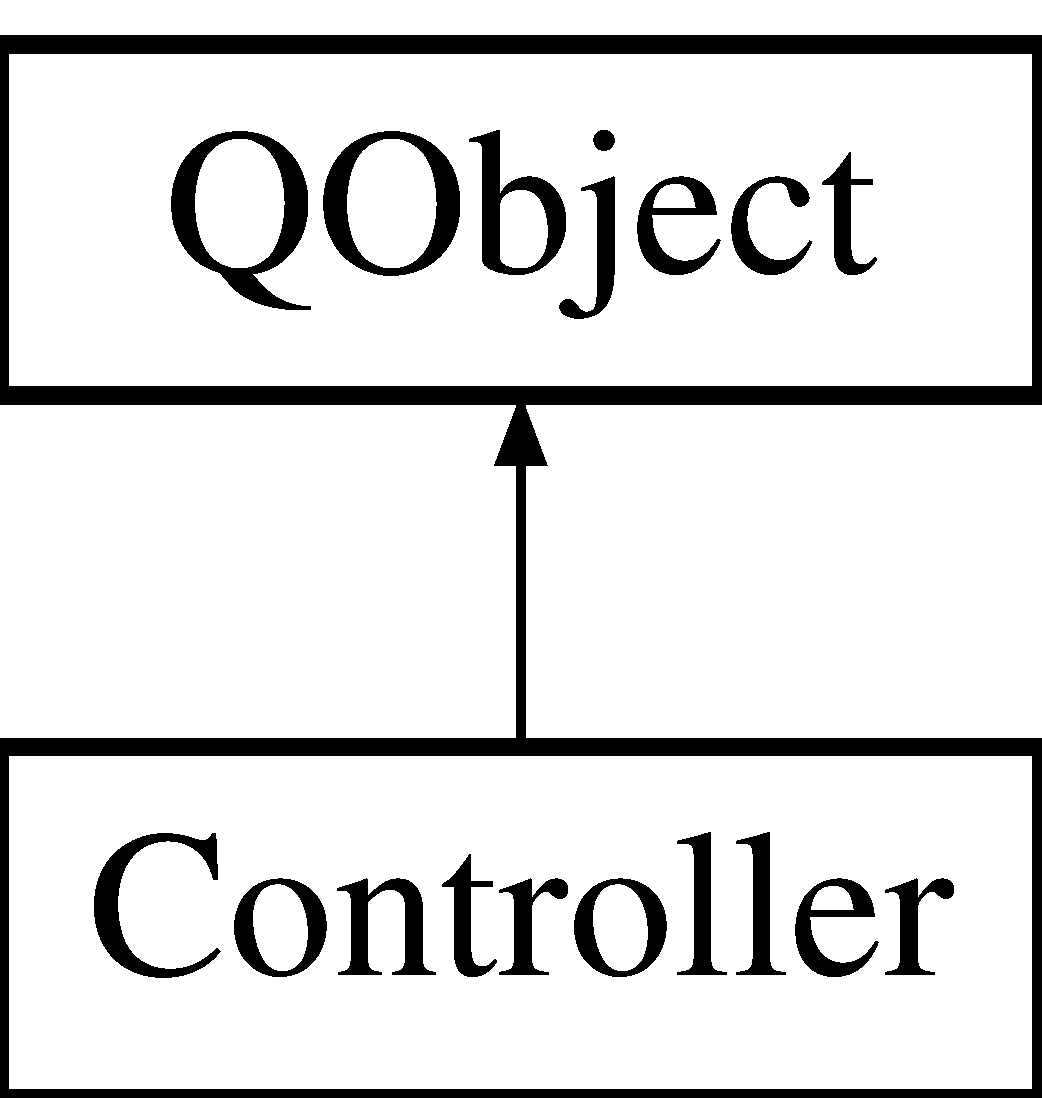
\includegraphics[height=2.000000cm]{class_controller}
\end{center}
\end{figure}
\subsection*{Public Slots}
\begin{DoxyCompactItemize}
\item 
void {\bf add\-Task\-Next} (int id, std\-::string question, std\-::string answer)
\begin{DoxyCompactList}\small\item\em add current task when we click next in course creator \end{DoxyCompactList}\item 
void {\bf add\-Task\-Back} (int id, std\-::string question, std\-::string answer)
\begin{DoxyCompactList}\small\item\em add current task when we click back in course creator \end{DoxyCompactList}\item 
void {\bf add\-Last\-Task} (int id, std\-::string question, std\-::string answer)
\begin{DoxyCompactList}\small\item\em add current task when we click save in course creator \end{DoxyCompactList}\item 
void {\bf add\-Save\-Course} (std\-::string name\-Of\-File)
\begin{DoxyCompactList}\small\item\em set course in creator \end{DoxyCompactList}\item 
void {\bf add\-List\-Of\-Files} ()
\begin{DoxyCompactList}\small\item\em set list names of courses \end{DoxyCompactList}\item 
void {\bf add\-Choose\-Course} (std\-::string course, bool flag)
\begin{DoxyCompactList}\small\item\em show chosen course \end{DoxyCompactList}\item 
void {\bf add\-Close\-Any\-Window} ()
\begin{DoxyCompactList}\small\item\em close window \end{DoxyCompactList}\item 
void {\bf delete\-Choose\-Course} (std\-::string course)
\begin{DoxyCompactList}\small\item\em when delete button clicked \end{DoxyCompactList}\item 
void {\bf compute\-Mark\-For\-Open} (int, std\-::string, std\-::string)
\begin{DoxyCompactList}\small\item\em used to count mark for open questions \end{DoxyCompactList}\item 
void {\bf compute\-Mark\-For\-Close} (int, vector$<$ bool $>$, vector$<$ bool $>$)
\begin{DoxyCompactList}\small\item\em used to count mark for close questions \end{DoxyCompactList}\item 
void {\bf end\-Course\-Judge} (vector$<$ int $>$, std\-::string)
\begin{DoxyCompactList}\small\item\em used to judge the course \end{DoxyCompactList}\item 
void {\bf add\-Choose\-Course\-Continue} (std\-::string name)
\begin{DoxyCompactList}\small\item\em used when Continue course clicked \end{DoxyCompactList}\item 
void {\bf add\-End\-Course} (vector$<$ int $>$, std\-::string)
\begin{DoxyCompactList}\small\item\em end of course \end{DoxyCompactList}\end{DoxyCompactItemize}
\subsection*{Signals}
\begin{DoxyCompactItemize}
\item 
void {\bf error} (std\-::string)
\begin{DoxyCompactList}\small\item\em emit when we catch exception. \end{DoxyCompactList}\item 
void {\bf go\-Next} (int id, std\-::string question, std\-::string answer)
\begin{DoxyCompactList}\small\item\em emit when we create course and go to next question. It contains task id,question and answer. \end{DoxyCompactList}\item 
void {\bf close\-Creator} ()
\begin{DoxyCompactList}\small\item\em emit when we save course to close creator window \end{DoxyCompactList}\item 
void {\bf get\-List\-Of\-Courses} (std\-::vector$<$ std\-::string $>$)
\begin{DoxyCompactList}\small\item\em emit list of names xml files with courses \end{DoxyCompactList}\item 
void {\bf close\-Start\-Window} ()
\begin{DoxyCompactList}\small\item\em emit when we choose course to close window \end{DoxyCompactList}\item 
void {\bf enabled\-Main\-Window} ()
\begin{DoxyCompactList}\small\item\em set enable main window when any other window close \end{DoxyCompactList}\item 
void {\bf emit\-Question\-Card\-List} (vector$<$ {\bf P\-Qcard} $>$, std\-::string)
\begin{DoxyCompactList}\small\item\em emit Question Card List and name of current course \end{DoxyCompactList}\item 
void {\bf emit\-Question\-Card\-List\-Continue} (vector$<$ {\bf P\-Qcard} $>$, std\-::string)
\begin{DoxyCompactList}\small\item\em emit when choosed option Contiunue \end{DoxyCompactList}\item 
void {\bf emit\-Suggested\-Mark} (int)
\begin{DoxyCompactList}\small\item\em emit suggested mark counted by computer \end{DoxyCompactList}\item 
void {\bf show\-Stats} (vector$<$ int $>$)
\begin{DoxyCompactList}\small\item\em emit marks to statistic \end{DoxyCompactList}\end{DoxyCompactItemize}
\subsection*{Public Member Functions}
\begin{DoxyCompactItemize}
\item 
{\bf Controller} ()
\item 
{\bf $\sim$\-Controller} ()
\item 
void {\bf connect\-View} ({\bf View} $\ast$view)
\begin{DoxyCompactList}\small\item\em connect \doxyref{View}{p.}{class_view} to controller \end{DoxyCompactList}\end{DoxyCompactItemize}
\subsection*{Private Attributes}
\begin{DoxyCompactItemize}
\item 
{\bf View} $\ast$ {\bf view\-\_\-}
\item 
{\bf Model} $\ast$ {\bf model\-\_\-}
\end{DoxyCompactItemize}


\subsection{Detailed Description}
Class represents \doxyref{Controller}{p.}{class_controller} in M\-V\-C. It communicate between \doxyref{Model}{p.}{class_model} and View.\-It respond on user actions, calls up methods from \doxyref{Model}{p.}{class_model} to get data. \doxyref{Controller}{p.}{class_controller} emits signals to inform \doxyref{View}{p.}{class_view} about change model state. \begin{DoxyAuthor}{Author}
Piotr Maleci \& Michal Daniluk 
\end{DoxyAuthor}


\subsection{Constructor \& Destructor Documentation}
\index{Controller@{Controller}!Controller@{Controller}}
\index{Controller@{Controller}!Controller@{Controller}}
\subsubsection[{Controller}]{\setlength{\rightskip}{0pt plus 5cm}Controller\-::\-Controller (
\begin{DoxyParamCaption}
{}
\end{DoxyParamCaption}
)\hspace{0.3cm}{\ttfamily [explicit]}}\label{class_controller_a95c56822d667e94b031451729ce069a9}
\index{Controller@{Controller}!$\sim$\-Controller@{$\sim$\-Controller}}
\index{$\sim$\-Controller@{$\sim$\-Controller}!Controller@{Controller}}
\subsubsection[{$\sim$\-Controller}]{\setlength{\rightskip}{0pt plus 5cm}Controller\-::$\sim$\-Controller (
\begin{DoxyParamCaption}
{}
\end{DoxyParamCaption}
)}\label{class_controller_a0ab87934c4f7a266cfdb86e0f36bc1b5}


\subsection{Member Function Documentation}
\index{Controller@{Controller}!add\-Choose\-Course@{add\-Choose\-Course}}
\index{add\-Choose\-Course@{add\-Choose\-Course}!Controller@{Controller}}
\subsubsection[{add\-Choose\-Course}]{\setlength{\rightskip}{0pt plus 5cm}void Controller\-::add\-Choose\-Course (
\begin{DoxyParamCaption}
\item[{std\-::string}]{course, }
\item[{bool}]{flag}
\end{DoxyParamCaption}
)\hspace{0.3cm}{\ttfamily [slot]}}\label{class_controller_a237cc194575e06bb1838bc4ef9066f60}


show chosen course 

\index{Controller@{Controller}!add\-Choose\-Course\-Continue@{add\-Choose\-Course\-Continue}}
\index{add\-Choose\-Course\-Continue@{add\-Choose\-Course\-Continue}!Controller@{Controller}}
\subsubsection[{add\-Choose\-Course\-Continue}]{\setlength{\rightskip}{0pt plus 5cm}void Controller\-::add\-Choose\-Course\-Continue (
\begin{DoxyParamCaption}
\item[{std\-::string}]{name}
\end{DoxyParamCaption}
)\hspace{0.3cm}{\ttfamily [slot]}}\label{class_controller_aaecc9270c5eb4129960a6de1fc7d9898}


used when Continue course clicked 

\index{Controller@{Controller}!add\-Close\-Any\-Window@{add\-Close\-Any\-Window}}
\index{add\-Close\-Any\-Window@{add\-Close\-Any\-Window}!Controller@{Controller}}
\subsubsection[{add\-Close\-Any\-Window}]{\setlength{\rightskip}{0pt plus 5cm}void Controller\-::add\-Close\-Any\-Window (
\begin{DoxyParamCaption}
{}
\end{DoxyParamCaption}
)\hspace{0.3cm}{\ttfamily [slot]}}\label{class_controller_a7ee8a4eb7d7f0a8e786f09587bb9607f}


close window 

\index{Controller@{Controller}!add\-End\-Course@{add\-End\-Course}}
\index{add\-End\-Course@{add\-End\-Course}!Controller@{Controller}}
\subsubsection[{add\-End\-Course}]{\setlength{\rightskip}{0pt plus 5cm}void Controller\-::add\-End\-Course (
\begin{DoxyParamCaption}
\item[{vector$<$ int $>$}]{marks, }
\item[{std\-::string}]{name}
\end{DoxyParamCaption}
)\hspace{0.3cm}{\ttfamily [slot]}}\label{class_controller_a50afe16c31586a0be61d140a76c687f5}


end of course 

\index{Controller@{Controller}!add\-Last\-Task@{add\-Last\-Task}}
\index{add\-Last\-Task@{add\-Last\-Task}!Controller@{Controller}}
\subsubsection[{add\-Last\-Task}]{\setlength{\rightskip}{0pt plus 5cm}void Controller\-::add\-Last\-Task (
\begin{DoxyParamCaption}
\item[{int}]{id, }
\item[{std\-::string}]{question, }
\item[{std\-::string}]{answer}
\end{DoxyParamCaption}
)\hspace{0.3cm}{\ttfamily [slot]}}\label{class_controller_a9a38ec67594e89557e84ca53c07e6c36}


add current task when we click save in course creator 

\index{Controller@{Controller}!add\-List\-Of\-Files@{add\-List\-Of\-Files}}
\index{add\-List\-Of\-Files@{add\-List\-Of\-Files}!Controller@{Controller}}
\subsubsection[{add\-List\-Of\-Files}]{\setlength{\rightskip}{0pt plus 5cm}void Controller\-::add\-List\-Of\-Files (
\begin{DoxyParamCaption}
{}
\end{DoxyParamCaption}
)\hspace{0.3cm}{\ttfamily [slot]}}\label{class_controller_a159c919c1a9797224d6ba6f04b44dc90}


set list names of courses 

\index{Controller@{Controller}!add\-Save\-Course@{add\-Save\-Course}}
\index{add\-Save\-Course@{add\-Save\-Course}!Controller@{Controller}}
\subsubsection[{add\-Save\-Course}]{\setlength{\rightskip}{0pt plus 5cm}void Controller\-::add\-Save\-Course (
\begin{DoxyParamCaption}
\item[{std\-::string}]{name\-Of\-File}
\end{DoxyParamCaption}
)\hspace{0.3cm}{\ttfamily [slot]}}\label{class_controller_a39de4f27d21a469e6582a6fe02ad2bcf}


set course in creator 

\index{Controller@{Controller}!add\-Task\-Back@{add\-Task\-Back}}
\index{add\-Task\-Back@{add\-Task\-Back}!Controller@{Controller}}
\subsubsection[{add\-Task\-Back}]{\setlength{\rightskip}{0pt plus 5cm}void Controller\-::add\-Task\-Back (
\begin{DoxyParamCaption}
\item[{int}]{id, }
\item[{std\-::string}]{question, }
\item[{std\-::string}]{answer}
\end{DoxyParamCaption}
)\hspace{0.3cm}{\ttfamily [slot]}}\label{class_controller_ad705b15118fedced188479b8d8514457}


add current task when we click back in course creator 

\index{Controller@{Controller}!add\-Task\-Next@{add\-Task\-Next}}
\index{add\-Task\-Next@{add\-Task\-Next}!Controller@{Controller}}
\subsubsection[{add\-Task\-Next}]{\setlength{\rightskip}{0pt plus 5cm}void Controller\-::add\-Task\-Next (
\begin{DoxyParamCaption}
\item[{int}]{id, }
\item[{std\-::string}]{question, }
\item[{std\-::string}]{answer}
\end{DoxyParamCaption}
)\hspace{0.3cm}{\ttfamily [slot]}}\label{class_controller_a8eb5e6f7512d5ee9c69467192bb5097a}


add current task when we click next in course creator 

\index{Controller@{Controller}!close\-Creator@{close\-Creator}}
\index{close\-Creator@{close\-Creator}!Controller@{Controller}}
\subsubsection[{close\-Creator}]{\setlength{\rightskip}{0pt plus 5cm}void Controller\-::close\-Creator (
\begin{DoxyParamCaption}
{}
\end{DoxyParamCaption}
)\hspace{0.3cm}{\ttfamily [signal]}}\label{class_controller_aa6ba203f8be9b921e0fc7ec4bc412241}


emit when we save course to close creator window 

\index{Controller@{Controller}!close\-Start\-Window@{close\-Start\-Window}}
\index{close\-Start\-Window@{close\-Start\-Window}!Controller@{Controller}}
\subsubsection[{close\-Start\-Window}]{\setlength{\rightskip}{0pt plus 5cm}void Controller\-::close\-Start\-Window (
\begin{DoxyParamCaption}
{}
\end{DoxyParamCaption}
)\hspace{0.3cm}{\ttfamily [signal]}}\label{class_controller_a7a0ba393140c98402bdec5b9d0095a32}


emit when we choose course to close window 

\index{Controller@{Controller}!compute\-Mark\-For\-Close@{compute\-Mark\-For\-Close}}
\index{compute\-Mark\-For\-Close@{compute\-Mark\-For\-Close}!Controller@{Controller}}
\subsubsection[{compute\-Mark\-For\-Close}]{\setlength{\rightskip}{0pt plus 5cm}void Controller\-::compute\-Mark\-For\-Close (
\begin{DoxyParamCaption}
\item[{int}]{type, }
\item[{vector$<$ bool $>$}]{user, }
\item[{vector$<$ bool $>$}]{correct}
\end{DoxyParamCaption}
)\hspace{0.3cm}{\ttfamily [slot]}}\label{class_controller_a84608057a98bc83693d347e14c8a731a}


used to count mark for close questions 

\index{Controller@{Controller}!compute\-Mark\-For\-Open@{compute\-Mark\-For\-Open}}
\index{compute\-Mark\-For\-Open@{compute\-Mark\-For\-Open}!Controller@{Controller}}
\subsubsection[{compute\-Mark\-For\-Open}]{\setlength{\rightskip}{0pt plus 5cm}void Controller\-::compute\-Mark\-For\-Open (
\begin{DoxyParamCaption}
\item[{int}]{type, }
\item[{std\-::string}]{user, }
\item[{std\-::string}]{correct}
\end{DoxyParamCaption}
)\hspace{0.3cm}{\ttfamily [slot]}}\label{class_controller_aa7e31ff2ca95a9aced78c246e9cc2cc1}


used to count mark for open questions 

\index{Controller@{Controller}!connect\-View@{connect\-View}}
\index{connect\-View@{connect\-View}!Controller@{Controller}}
\subsubsection[{connect\-View}]{\setlength{\rightskip}{0pt plus 5cm}void Controller\-::connect\-View (
\begin{DoxyParamCaption}
\item[{{\bf View} $\ast$}]{view}
\end{DoxyParamCaption}
)}\label{class_controller_a50d72513cf40c383e6dc8cb58c9a9c2a}


connect \doxyref{View}{p.}{class_view} to controller 

\index{Controller@{Controller}!delete\-Choose\-Course@{delete\-Choose\-Course}}
\index{delete\-Choose\-Course@{delete\-Choose\-Course}!Controller@{Controller}}
\subsubsection[{delete\-Choose\-Course}]{\setlength{\rightskip}{0pt plus 5cm}void Controller\-::delete\-Choose\-Course (
\begin{DoxyParamCaption}
\item[{std\-::string}]{course}
\end{DoxyParamCaption}
)\hspace{0.3cm}{\ttfamily [slot]}}\label{class_controller_a2d739cc72ac8d39cba976072cc26d98d}


when delete button clicked 

\index{Controller@{Controller}!emit\-Question\-Card\-List@{emit\-Question\-Card\-List}}
\index{emit\-Question\-Card\-List@{emit\-Question\-Card\-List}!Controller@{Controller}}
\subsubsection[{emit\-Question\-Card\-List}]{\setlength{\rightskip}{0pt plus 5cm}void Controller\-::emit\-Question\-Card\-List (
\begin{DoxyParamCaption}
\item[{vector$<$ {\bf P\-Qcard} $>$}]{\-\_\-t1, }
\item[{std\-::string}]{\-\_\-t2}
\end{DoxyParamCaption}
)\hspace{0.3cm}{\ttfamily [signal]}}\label{class_controller_ae1289fb5e1e3525ac96db0d136afe509}


emit Question Card List and name of current course 

\index{Controller@{Controller}!emit\-Question\-Card\-List\-Continue@{emit\-Question\-Card\-List\-Continue}}
\index{emit\-Question\-Card\-List\-Continue@{emit\-Question\-Card\-List\-Continue}!Controller@{Controller}}
\subsubsection[{emit\-Question\-Card\-List\-Continue}]{\setlength{\rightskip}{0pt plus 5cm}void Controller\-::emit\-Question\-Card\-List\-Continue (
\begin{DoxyParamCaption}
\item[{vector$<$ {\bf P\-Qcard} $>$}]{\-\_\-t1, }
\item[{std\-::string}]{\-\_\-t2}
\end{DoxyParamCaption}
)\hspace{0.3cm}{\ttfamily [signal]}}\label{class_controller_aa25e21d1682c6e8207dadc2e792a30df}


emit when choosed option Contiunue 

\index{Controller@{Controller}!emit\-Suggested\-Mark@{emit\-Suggested\-Mark}}
\index{emit\-Suggested\-Mark@{emit\-Suggested\-Mark}!Controller@{Controller}}
\subsubsection[{emit\-Suggested\-Mark}]{\setlength{\rightskip}{0pt plus 5cm}void Controller\-::emit\-Suggested\-Mark (
\begin{DoxyParamCaption}
\item[{int}]{\-\_\-t1}
\end{DoxyParamCaption}
)\hspace{0.3cm}{\ttfamily [signal]}}\label{class_controller_a3ef7f656abd8c7e69eeacdce849ce12d}


emit suggested mark counted by computer 

\index{Controller@{Controller}!enabled\-Main\-Window@{enabled\-Main\-Window}}
\index{enabled\-Main\-Window@{enabled\-Main\-Window}!Controller@{Controller}}
\subsubsection[{enabled\-Main\-Window}]{\setlength{\rightskip}{0pt plus 5cm}void Controller\-::enabled\-Main\-Window (
\begin{DoxyParamCaption}
{}
\end{DoxyParamCaption}
)\hspace{0.3cm}{\ttfamily [signal]}}\label{class_controller_adedf10a18e2b5c84ba1683928d5a2f68}


set enable main window when any other window close 

\index{Controller@{Controller}!end\-Course\-Judge@{end\-Course\-Judge}}
\index{end\-Course\-Judge@{end\-Course\-Judge}!Controller@{Controller}}
\subsubsection[{end\-Course\-Judge}]{\setlength{\rightskip}{0pt plus 5cm}void Controller\-::end\-Course\-Judge (
\begin{DoxyParamCaption}
\item[{vector$<$ int $>$}]{, }
\item[{std\-::string}]{}
\end{DoxyParamCaption}
)\hspace{0.3cm}{\ttfamily [slot]}}\label{class_controller_a0d0a8ff395bc737b333d3c7abb24bfb5}


used to judge the course 

\index{Controller@{Controller}!error@{error}}
\index{error@{error}!Controller@{Controller}}
\subsubsection[{error}]{\setlength{\rightskip}{0pt plus 5cm}void Controller\-::error (
\begin{DoxyParamCaption}
\item[{std\-::string}]{\-\_\-t1}
\end{DoxyParamCaption}
)\hspace{0.3cm}{\ttfamily [signal]}}\label{class_controller_a74dc9631de09ae2b86e61bf3ba4f3eea}


emit when we catch exception. 

\index{Controller@{Controller}!get\-List\-Of\-Courses@{get\-List\-Of\-Courses}}
\index{get\-List\-Of\-Courses@{get\-List\-Of\-Courses}!Controller@{Controller}}
\subsubsection[{get\-List\-Of\-Courses}]{\setlength{\rightskip}{0pt plus 5cm}void Controller\-::get\-List\-Of\-Courses (
\begin{DoxyParamCaption}
\item[{std\-::vector$<$ std\-::string $>$}]{\-\_\-t1}
\end{DoxyParamCaption}
)\hspace{0.3cm}{\ttfamily [signal]}}\label{class_controller_a0eb01297d58d5db2108c25d44c2d20b3}


emit list of names xml files with courses 

\index{Controller@{Controller}!go\-Next@{go\-Next}}
\index{go\-Next@{go\-Next}!Controller@{Controller}}
\subsubsection[{go\-Next}]{\setlength{\rightskip}{0pt plus 5cm}void Controller\-::go\-Next (
\begin{DoxyParamCaption}
\item[{int}]{id, }
\item[{std\-::string}]{question, }
\item[{std\-::string}]{answer}
\end{DoxyParamCaption}
)\hspace{0.3cm}{\ttfamily [signal]}}\label{class_controller_a3a46ebb0133dcfbb2a90470d6ac27832}


emit when we create course and go to next question. It contains task id,question and answer. 

\index{Controller@{Controller}!show\-Stats@{show\-Stats}}
\index{show\-Stats@{show\-Stats}!Controller@{Controller}}
\subsubsection[{show\-Stats}]{\setlength{\rightskip}{0pt plus 5cm}void Controller\-::show\-Stats (
\begin{DoxyParamCaption}
\item[{vector$<$ int $>$}]{\-\_\-t1}
\end{DoxyParamCaption}
)\hspace{0.3cm}{\ttfamily [signal]}}\label{class_controller_ae5e63eafb76d0755170bc771aa6b1e4c}


emit marks to statistic 



\subsection{Member Data Documentation}
\index{Controller@{Controller}!model\-\_\-@{model\-\_\-}}
\index{model\-\_\-@{model\-\_\-}!Controller@{Controller}}
\subsubsection[{model\-\_\-}]{\setlength{\rightskip}{0pt plus 5cm}{\bf Model}$\ast$ Controller\-::model\-\_\-\hspace{0.3cm}{\ttfamily [private]}}\label{class_controller_a883630e7bbe2b0e24a370c3122249d07}
\index{Controller@{Controller}!view\-\_\-@{view\-\_\-}}
\index{view\-\_\-@{view\-\_\-}!Controller@{Controller}}
\subsubsection[{view\-\_\-}]{\setlength{\rightskip}{0pt plus 5cm}{\bf View}$\ast$ Controller\-::view\-\_\-\hspace{0.3cm}{\ttfamily [private]}}\label{class_controller_a02f83722f9e5b258d78cffda10cd4489}


The documentation for this class was generated from the following files\-:\begin{DoxyCompactItemize}
\item 
Projekt\-Z\-P\-R/{\bf controller.\-h}\item 
Projekt\-Z\-P\-R/{\bf controller.\-cpp}\item 
Projekt\-Z\-P\-R/\-Generated\-Files/\-Debug/{\bf moc\-\_\-controller.\-cpp}\item 
Projekt\-Z\-P\-R/\-Generated\-Files/\-Release/{\bf moc\-\_\-controller.\-cpp}\item 
Projekt\-Z\-P\-R/\-Generated\-Files/\-Testy\-Z\-P\-R/{\bf moc\-\_\-controller.\-cpp}\item 
Projekt\-Z\-P\-R/\-Generated\-Files/\-Testy\-Z\-P\-R2/{\bf moc\-\_\-controller.\-cpp}\end{DoxyCompactItemize}

\section{Course Class Reference}
\label{class_course}\index{Course@{Course}}


{\ttfamily \#include $<$course.\-h$>$}

\subsection*{Public Member Functions}
\begin{DoxyCompactItemize}
\item 
{\bf Course} (void)
\item 
{\bf $\sim$\-Course} ()
\item 
vector$<$ string $>$ {\bf get\-Questions} ()
\item 
vector$<$ string $>$ {\bf get\-Answers} ()
\item 
string {\bf get\-Questions} (int index)
\item 
string {\bf get\-Answers} (int index)
\item 
void {\bf set\-Questions} (int id, string question)
\item 
void {\bf set\-Answers} (int id, string answer)
\item 
void {\bf write\-To\-X\-M\-L} (std\-::string name\-Of\-File)
\end{DoxyCompactItemize}
\subsection*{Private Attributes}
\begin{DoxyCompactItemize}
\item 
vector$<$ string $>$ {\bf questions}
\item 
vector$<$ string $>$ {\bf answers}
\item 
int {\bf number\-Of\-Questions\-\_\-}
\end{DoxyCompactItemize}


\subsection{Detailed Description}
Class represents logic of course creator \begin{DoxyAuthor}{Author}
Piotr Maleci \& Michal Daniluk 
\end{DoxyAuthor}


\subsection{Constructor \& Destructor Documentation}
\index{Course@{Course}!Course@{Course}}
\index{Course@{Course}!Course@{Course}}
\subsubsection[{Course}]{\setlength{\rightskip}{0pt plus 5cm}Course\-::\-Course (
\begin{DoxyParamCaption}
\item[{void}]{}
\end{DoxyParamCaption}
)}\label{class_course_a47049fe05b86e2e9443a951ac596d41a}
\index{Course@{Course}!$\sim$\-Course@{$\sim$\-Course}}
\index{$\sim$\-Course@{$\sim$\-Course}!Course@{Course}}
\subsubsection[{$\sim$\-Course}]{\setlength{\rightskip}{0pt plus 5cm}Course\-::$\sim$\-Course (
\begin{DoxyParamCaption}
{}
\end{DoxyParamCaption}
)}\label{class_course_aa9038f2e129526920037dda9e76d69d0}


\subsection{Member Function Documentation}
\index{Course@{Course}!get\-Answers@{get\-Answers}}
\index{get\-Answers@{get\-Answers}!Course@{Course}}
\subsubsection[{get\-Answers}]{\setlength{\rightskip}{0pt plus 5cm}vector$<$string$>$ Course\-::get\-Answers (
\begin{DoxyParamCaption}
{}
\end{DoxyParamCaption}
)\hspace{0.3cm}{\ttfamily [inline]}}\label{class_course_adcc45874b4d669ccb8f61fa5b6b5ccea}
\index{Course@{Course}!get\-Answers@{get\-Answers}}
\index{get\-Answers@{get\-Answers}!Course@{Course}}
\subsubsection[{get\-Answers}]{\setlength{\rightskip}{0pt plus 5cm}string Course\-::get\-Answers (
\begin{DoxyParamCaption}
\item[{int}]{index}
\end{DoxyParamCaption}
)}\label{class_course_a785e0eabf6d5437b354f2a1bd719225c}
\index{Course@{Course}!get\-Questions@{get\-Questions}}
\index{get\-Questions@{get\-Questions}!Course@{Course}}
\subsubsection[{get\-Questions}]{\setlength{\rightskip}{0pt plus 5cm}vector$<$string$>$ Course\-::get\-Questions (
\begin{DoxyParamCaption}
{}
\end{DoxyParamCaption}
)\hspace{0.3cm}{\ttfamily [inline]}}\label{class_course_a503efffe9d1f3949618efaa71ead2442}
\index{Course@{Course}!get\-Questions@{get\-Questions}}
\index{get\-Questions@{get\-Questions}!Course@{Course}}
\subsubsection[{get\-Questions}]{\setlength{\rightskip}{0pt plus 5cm}string Course\-::get\-Questions (
\begin{DoxyParamCaption}
\item[{int}]{index}
\end{DoxyParamCaption}
)}\label{class_course_a88a7a4f9b8a9c6eac2cde76a735b6542}
\index{Course@{Course}!set\-Answers@{set\-Answers}}
\index{set\-Answers@{set\-Answers}!Course@{Course}}
\subsubsection[{set\-Answers}]{\setlength{\rightskip}{0pt plus 5cm}void Course\-::set\-Answers (
\begin{DoxyParamCaption}
\item[{int}]{id, }
\item[{string}]{answer}
\end{DoxyParamCaption}
)}\label{class_course_a74fd02306d58cab833d028e16fc608b3}
\index{Course@{Course}!set\-Questions@{set\-Questions}}
\index{set\-Questions@{set\-Questions}!Course@{Course}}
\subsubsection[{set\-Questions}]{\setlength{\rightskip}{0pt plus 5cm}void Course\-::set\-Questions (
\begin{DoxyParamCaption}
\item[{int}]{id, }
\item[{string}]{question}
\end{DoxyParamCaption}
)}\label{class_course_a8bae174780438b864a1a1f192f823e7b}
\index{Course@{Course}!write\-To\-X\-M\-L@{write\-To\-X\-M\-L}}
\index{write\-To\-X\-M\-L@{write\-To\-X\-M\-L}!Course@{Course}}
\subsubsection[{write\-To\-X\-M\-L}]{\setlength{\rightskip}{0pt plus 5cm}void Course\-::write\-To\-X\-M\-L (
\begin{DoxyParamCaption}
\item[{std\-::string}]{name\-Of\-File}
\end{DoxyParamCaption}
)}\label{class_course_aea8151ddbda24f35a0449fa1b360581c}


\subsection{Member Data Documentation}
\index{Course@{Course}!answers@{answers}}
\index{answers@{answers}!Course@{Course}}
\subsubsection[{answers}]{\setlength{\rightskip}{0pt plus 5cm}vector$<$string$>$ Course\-::answers\hspace{0.3cm}{\ttfamily [private]}}\label{class_course_ab29e40631a77c3e57f6d0d1597cda1e8}
\index{Course@{Course}!number\-Of\-Questions\-\_\-@{number\-Of\-Questions\-\_\-}}
\index{number\-Of\-Questions\-\_\-@{number\-Of\-Questions\-\_\-}!Course@{Course}}
\subsubsection[{number\-Of\-Questions\-\_\-}]{\setlength{\rightskip}{0pt plus 5cm}int Course\-::number\-Of\-Questions\-\_\-\hspace{0.3cm}{\ttfamily [private]}}\label{class_course_ac8be6684d56f82b3b1022461f98f50c1}
\index{Course@{Course}!questions@{questions}}
\index{questions@{questions}!Course@{Course}}
\subsubsection[{questions}]{\setlength{\rightskip}{0pt plus 5cm}vector$<$string$>$ Course\-::questions\hspace{0.3cm}{\ttfamily [private]}}\label{class_course_a7e4549fa40ccc6fbb2caacec4abee7b8}


The documentation for this class was generated from the following files\-:\begin{DoxyCompactItemize}
\item 
Projekt\-Z\-P\-R/{\bf course.\-h}\item 
Projekt\-Z\-P\-R/{\bf course.\-cpp}\end{DoxyCompactItemize}

\section{Create\-Test Class Reference}
\label{class_create_test}\index{Create\-Test@{Create\-Test}}


{\ttfamily \#include $<$createtest.\-h$>$}

Inheritance diagram for Create\-Test\-:\begin{figure}[H]
\begin{center}
\leavevmode
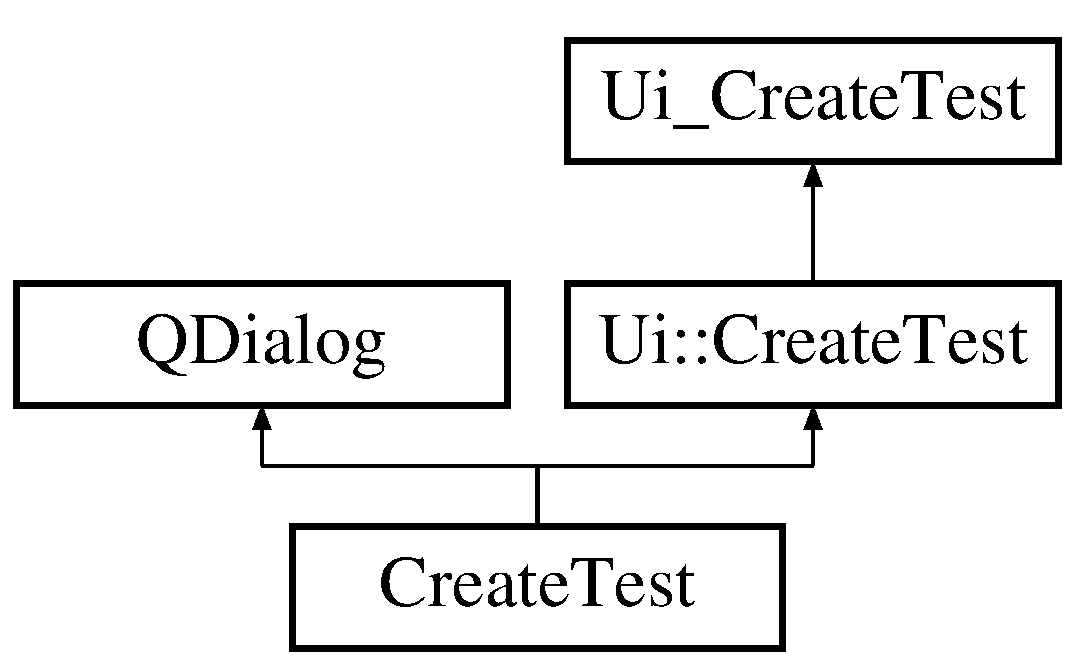
\includegraphics[height=3.000000cm]{class_create_test}
\end{center}
\end{figure}
\subsection*{Public Slots}
\begin{DoxyCompactItemize}
\item 
void {\bf refresh\-Task} (int number, std\-::string question, std\-::string answer)
\begin{DoxyCompactList}\small\item\em refresh task when we back to previus task, wchich we agreed. \end{DoxyCompactList}\item 
void {\bf current\-Changed\-Slot} (int index)
\begin{DoxyCompactList}\small\item\em show waring message when we want to change type of answer when we wrote one of them \end{DoxyCompactList}\item 
void {\bf close\-Window} ()
\end{DoxyCompactItemize}
\subsection*{Signals}
\begin{DoxyCompactItemize}
\item 
void {\bf set\-Task\-Next} (int id, std\-::string question, std\-::string answer)
\begin{DoxyCompactList}\small\item\em emit when we click next to set current task \end{DoxyCompactList}\item 
void {\bf set\-Task\-Back} (int id, std\-::string question, std\-::string answer)
\begin{DoxyCompactList}\small\item\em emit when we click back to set current task \end{DoxyCompactList}\item 
void {\bf set\-Last\-Task} (int id, std\-::string question, std\-::string answer)
\begin{DoxyCompactList}\small\item\em emit when we click save to set last task \end{DoxyCompactList}\item 
void {\bf save\-Course} (std\-::string)
\item 
void {\bf close\-Creator} ()
\end{DoxyCompactItemize}
\subsection*{Public Member Functions}
\begin{DoxyCompactItemize}
\item 
{\bf Create\-Test} ({\bf Controller} $\ast$controller, {\bf View} $\ast$parent=N\-U\-L\-L)
\item 
{\bf $\sim$\-Create\-Test} ()
\item 
void {\bf close\-Event} (Q\-Close\-Event $\ast$event)
\end{DoxyCompactItemize}
\subsection*{Private Slots}
\begin{DoxyCompactItemize}
\item 
void {\bf on\-\_\-next\-\_\-clicked} ()
\item 
void {\bf on\-\_\-back\-\_\-clicked} ()
\item 
void {\bf on\-\_\-save\-\_\-clicked} ()
\item 
void {\bf on\-\_\-help\-\_\-clicked} ()
\end{DoxyCompactItemize}
\subsection*{Private Member Functions}
\begin{DoxyCompactItemize}
\item 
void {\bf get\-Task} ()
\item 
void {\bf current\-Changed\-Tab} ()
\end{DoxyCompactItemize}
\subsection*{Private Attributes}
\begin{DoxyCompactItemize}
\item 
{\bf View} $\ast$ {\bf my\-View\-\_\-}
\item 
{\bf Controller} $\ast$ {\bf my\-Controller\-\_\-}
\item 
int {\bf number\-\_\-}
\item 
string {\bf answer\-\_\-}
\item 
string {\bf question\-\_\-}
\item 
int {\bf number\-Of\-Questions\-\_\-}
\item 
bool {\bf is\-Next\-Or\-Back\-\_\-}
\end{DoxyCompactItemize}
\subsection*{Additional Inherited Members}


\subsection{Detailed Description}
Class represents test creator dialog. \begin{DoxyAuthor}{Author}
Piotr Maleci \& Michal Daniluk 
\end{DoxyAuthor}


\subsection{Constructor \& Destructor Documentation}
\index{Create\-Test@{Create\-Test}!Create\-Test@{Create\-Test}}
\index{Create\-Test@{Create\-Test}!CreateTest@{Create\-Test}}
\subsubsection[{Create\-Test}]{\setlength{\rightskip}{0pt plus 5cm}Create\-Test\-::\-Create\-Test (
\begin{DoxyParamCaption}
\item[{{\bf Controller} $\ast$}]{controller, }
\item[{{\bf View} $\ast$}]{parent = {\ttfamily NULL}}
\end{DoxyParamCaption}
)}\label{class_create_test_a6142a8b5db1b0b01b19cd32937744f1c}
\index{Create\-Test@{Create\-Test}!$\sim$\-Create\-Test@{$\sim$\-Create\-Test}}
\index{$\sim$\-Create\-Test@{$\sim$\-Create\-Test}!CreateTest@{Create\-Test}}
\subsubsection[{$\sim$\-Create\-Test}]{\setlength{\rightskip}{0pt plus 5cm}Create\-Test\-::$\sim$\-Create\-Test (
\begin{DoxyParamCaption}
{}
\end{DoxyParamCaption}
)}\label{class_create_test_ac9a712208a3a64f531ffbcec4aab07cc}


\subsection{Member Function Documentation}
\index{Create\-Test@{Create\-Test}!close\-Creator@{close\-Creator}}
\index{close\-Creator@{close\-Creator}!CreateTest@{Create\-Test}}
\subsubsection[{close\-Creator}]{\setlength{\rightskip}{0pt plus 5cm}void Create\-Test\-::close\-Creator (
\begin{DoxyParamCaption}
{}
\end{DoxyParamCaption}
)\hspace{0.3cm}{\ttfamily [signal]}}\label{class_create_test_ac3186d53855ebf1aa206323106682546}
\index{Create\-Test@{Create\-Test}!close\-Event@{close\-Event}}
\index{close\-Event@{close\-Event}!CreateTest@{Create\-Test}}
\subsubsection[{close\-Event}]{\setlength{\rightskip}{0pt plus 5cm}void Create\-Test\-::close\-Event (
\begin{DoxyParamCaption}
\item[{Q\-Close\-Event $\ast$}]{event}
\end{DoxyParamCaption}
)}\label{class_create_test_a92c077986e2df975c6d9efe585a1e7c2}
\index{Create\-Test@{Create\-Test}!close\-Window@{close\-Window}}
\index{close\-Window@{close\-Window}!CreateTest@{Create\-Test}}
\subsubsection[{close\-Window}]{\setlength{\rightskip}{0pt plus 5cm}void Create\-Test\-::close\-Window (
\begin{DoxyParamCaption}
{}
\end{DoxyParamCaption}
)\hspace{0.3cm}{\ttfamily [slot]}}\label{class_create_test_af628a165beae6e1abbc55cd69e7b9c5f}
\index{Create\-Test@{Create\-Test}!current\-Changed\-Slot@{current\-Changed\-Slot}}
\index{current\-Changed\-Slot@{current\-Changed\-Slot}!CreateTest@{Create\-Test}}
\subsubsection[{current\-Changed\-Slot}]{\setlength{\rightskip}{0pt plus 5cm}void Create\-Test\-::current\-Changed\-Slot (
\begin{DoxyParamCaption}
\item[{int}]{index}
\end{DoxyParamCaption}
)\hspace{0.3cm}{\ttfamily [slot]}}\label{class_create_test_a70a5c03eb200e142ce3d4ef335538809}


show waring message when we want to change type of answer when we wrote one of them 

\index{Create\-Test@{Create\-Test}!current\-Changed\-Tab@{current\-Changed\-Tab}}
\index{current\-Changed\-Tab@{current\-Changed\-Tab}!CreateTest@{Create\-Test}}
\subsubsection[{current\-Changed\-Tab}]{\setlength{\rightskip}{0pt plus 5cm}void Create\-Test\-::current\-Changed\-Tab (
\begin{DoxyParamCaption}
{}
\end{DoxyParamCaption}
)\hspace{0.3cm}{\ttfamily [private]}}\label{class_create_test_a62737a82d647c58f3355082fbfe9d2a6}
\index{Create\-Test@{Create\-Test}!get\-Task@{get\-Task}}
\index{get\-Task@{get\-Task}!CreateTest@{Create\-Test}}
\subsubsection[{get\-Task}]{\setlength{\rightskip}{0pt plus 5cm}void Create\-Test\-::get\-Task (
\begin{DoxyParamCaption}
{}
\end{DoxyParamCaption}
)\hspace{0.3cm}{\ttfamily [private]}}\label{class_create_test_a1fee6ebaf6cc6212e38530a89096aed2}
\index{Create\-Test@{Create\-Test}!on\-\_\-back\-\_\-clicked@{on\-\_\-back\-\_\-clicked}}
\index{on\-\_\-back\-\_\-clicked@{on\-\_\-back\-\_\-clicked}!CreateTest@{Create\-Test}}
\subsubsection[{on\-\_\-back\-\_\-clicked}]{\setlength{\rightskip}{0pt plus 5cm}void Create\-Test\-::on\-\_\-back\-\_\-clicked (
\begin{DoxyParamCaption}
{}
\end{DoxyParamCaption}
)\hspace{0.3cm}{\ttfamily [private]}, {\ttfamily [slot]}}\label{class_create_test_a8ee47f15d8316c43b6c488bfce79d160}
\index{Create\-Test@{Create\-Test}!on\-\_\-help\-\_\-clicked@{on\-\_\-help\-\_\-clicked}}
\index{on\-\_\-help\-\_\-clicked@{on\-\_\-help\-\_\-clicked}!CreateTest@{Create\-Test}}
\subsubsection[{on\-\_\-help\-\_\-clicked}]{\setlength{\rightskip}{0pt plus 5cm}void Create\-Test\-::on\-\_\-help\-\_\-clicked (
\begin{DoxyParamCaption}
{}
\end{DoxyParamCaption}
)\hspace{0.3cm}{\ttfamily [private]}, {\ttfamily [slot]}}\label{class_create_test_a3ca3818a63b6319a39c4e265a4f4544b}
\index{Create\-Test@{Create\-Test}!on\-\_\-next\-\_\-clicked@{on\-\_\-next\-\_\-clicked}}
\index{on\-\_\-next\-\_\-clicked@{on\-\_\-next\-\_\-clicked}!CreateTest@{Create\-Test}}
\subsubsection[{on\-\_\-next\-\_\-clicked}]{\setlength{\rightskip}{0pt plus 5cm}void Create\-Test\-::on\-\_\-next\-\_\-clicked (
\begin{DoxyParamCaption}
{}
\end{DoxyParamCaption}
)\hspace{0.3cm}{\ttfamily [private]}, {\ttfamily [slot]}}\label{class_create_test_a2801da6fd5810b2c03600780808c9618}
\index{Create\-Test@{Create\-Test}!on\-\_\-save\-\_\-clicked@{on\-\_\-save\-\_\-clicked}}
\index{on\-\_\-save\-\_\-clicked@{on\-\_\-save\-\_\-clicked}!CreateTest@{Create\-Test}}
\subsubsection[{on\-\_\-save\-\_\-clicked}]{\setlength{\rightskip}{0pt plus 5cm}void Create\-Test\-::on\-\_\-save\-\_\-clicked (
\begin{DoxyParamCaption}
{}
\end{DoxyParamCaption}
)\hspace{0.3cm}{\ttfamily [private]}, {\ttfamily [slot]}}\label{class_create_test_ab78df0a11684b34980b6e3294d81e94e}
\index{Create\-Test@{Create\-Test}!refresh\-Task@{refresh\-Task}}
\index{refresh\-Task@{refresh\-Task}!CreateTest@{Create\-Test}}
\subsubsection[{refresh\-Task}]{\setlength{\rightskip}{0pt plus 5cm}void Create\-Test\-::refresh\-Task (
\begin{DoxyParamCaption}
\item[{int}]{number, }
\item[{std\-::string}]{question, }
\item[{std\-::string}]{answer}
\end{DoxyParamCaption}
)\hspace{0.3cm}{\ttfamily [slot]}}\label{class_create_test_ad551555454f65522345371b5e046a190}


refresh task when we back to previus task, wchich we agreed. 

\index{Create\-Test@{Create\-Test}!save\-Course@{save\-Course}}
\index{save\-Course@{save\-Course}!CreateTest@{Create\-Test}}
\subsubsection[{save\-Course}]{\setlength{\rightskip}{0pt plus 5cm}void Create\-Test\-::save\-Course (
\begin{DoxyParamCaption}
\item[{std\-::string}]{\-\_\-t1}
\end{DoxyParamCaption}
)\hspace{0.3cm}{\ttfamily [signal]}}\label{class_create_test_a8b3b1550a554ca6bba3e96cb4ae48fd5}
\index{Create\-Test@{Create\-Test}!set\-Last\-Task@{set\-Last\-Task}}
\index{set\-Last\-Task@{set\-Last\-Task}!CreateTest@{Create\-Test}}
\subsubsection[{set\-Last\-Task}]{\setlength{\rightskip}{0pt plus 5cm}void Create\-Test\-::set\-Last\-Task (
\begin{DoxyParamCaption}
\item[{int}]{id, }
\item[{std\-::string}]{question, }
\item[{std\-::string}]{answer}
\end{DoxyParamCaption}
)\hspace{0.3cm}{\ttfamily [signal]}}\label{class_create_test_a056ce41fe0e8fc89a8e84f95869a4658}


emit when we click save to set last task 

\index{Create\-Test@{Create\-Test}!set\-Task\-Back@{set\-Task\-Back}}
\index{set\-Task\-Back@{set\-Task\-Back}!CreateTest@{Create\-Test}}
\subsubsection[{set\-Task\-Back}]{\setlength{\rightskip}{0pt plus 5cm}void Create\-Test\-::set\-Task\-Back (
\begin{DoxyParamCaption}
\item[{int}]{id, }
\item[{std\-::string}]{question, }
\item[{std\-::string}]{answer}
\end{DoxyParamCaption}
)\hspace{0.3cm}{\ttfamily [signal]}}\label{class_create_test_ab6be0fd1e22f66a06e36cd33c82bb731}


emit when we click back to set current task 

\index{Create\-Test@{Create\-Test}!set\-Task\-Next@{set\-Task\-Next}}
\index{set\-Task\-Next@{set\-Task\-Next}!CreateTest@{Create\-Test}}
\subsubsection[{set\-Task\-Next}]{\setlength{\rightskip}{0pt plus 5cm}void Create\-Test\-::set\-Task\-Next (
\begin{DoxyParamCaption}
\item[{int}]{id, }
\item[{std\-::string}]{question, }
\item[{std\-::string}]{answer}
\end{DoxyParamCaption}
)\hspace{0.3cm}{\ttfamily [signal]}}\label{class_create_test_a47710afff9c1b0f825ad47dc50b8955c}


emit when we click next to set current task 



\subsection{Member Data Documentation}
\index{Create\-Test@{Create\-Test}!answer\-\_\-@{answer\-\_\-}}
\index{answer\-\_\-@{answer\-\_\-}!CreateTest@{Create\-Test}}
\subsubsection[{answer\-\_\-}]{\setlength{\rightskip}{0pt plus 5cm}string Create\-Test\-::answer\-\_\-\hspace{0.3cm}{\ttfamily [private]}}\label{class_create_test_a97330835e7e0cb416f87bdc6ad0e7471}
\index{Create\-Test@{Create\-Test}!is\-Next\-Or\-Back\-\_\-@{is\-Next\-Or\-Back\-\_\-}}
\index{is\-Next\-Or\-Back\-\_\-@{is\-Next\-Or\-Back\-\_\-}!CreateTest@{Create\-Test}}
\subsubsection[{is\-Next\-Or\-Back\-\_\-}]{\setlength{\rightskip}{0pt plus 5cm}bool Create\-Test\-::is\-Next\-Or\-Back\-\_\-\hspace{0.3cm}{\ttfamily [private]}}\label{class_create_test_a27f5feb19b16f62722cafa649b576b90}
\index{Create\-Test@{Create\-Test}!my\-Controller\-\_\-@{my\-Controller\-\_\-}}
\index{my\-Controller\-\_\-@{my\-Controller\-\_\-}!CreateTest@{Create\-Test}}
\subsubsection[{my\-Controller\-\_\-}]{\setlength{\rightskip}{0pt plus 5cm}{\bf Controller}$\ast$ Create\-Test\-::my\-Controller\-\_\-\hspace{0.3cm}{\ttfamily [private]}}\label{class_create_test_a685e8d1406bbf11fcfb8228402915c6e}
\index{Create\-Test@{Create\-Test}!my\-View\-\_\-@{my\-View\-\_\-}}
\index{my\-View\-\_\-@{my\-View\-\_\-}!CreateTest@{Create\-Test}}
\subsubsection[{my\-View\-\_\-}]{\setlength{\rightskip}{0pt plus 5cm}{\bf View}$\ast$ Create\-Test\-::my\-View\-\_\-\hspace{0.3cm}{\ttfamily [private]}}\label{class_create_test_a4960a53fd2fed242295e730805548b76}
\index{Create\-Test@{Create\-Test}!number\-\_\-@{number\-\_\-}}
\index{number\-\_\-@{number\-\_\-}!CreateTest@{Create\-Test}}
\subsubsection[{number\-\_\-}]{\setlength{\rightskip}{0pt plus 5cm}int Create\-Test\-::number\-\_\-\hspace{0.3cm}{\ttfamily [private]}}\label{class_create_test_ab807c29561c5fe6f5f6c9d34d7ab5fa7}
\index{Create\-Test@{Create\-Test}!number\-Of\-Questions\-\_\-@{number\-Of\-Questions\-\_\-}}
\index{number\-Of\-Questions\-\_\-@{number\-Of\-Questions\-\_\-}!CreateTest@{Create\-Test}}
\subsubsection[{number\-Of\-Questions\-\_\-}]{\setlength{\rightskip}{0pt plus 5cm}int Create\-Test\-::number\-Of\-Questions\-\_\-\hspace{0.3cm}{\ttfamily [private]}}\label{class_create_test_a4ab76bc4c6a46a1709d1f4a3d8ce0fb5}
\index{Create\-Test@{Create\-Test}!question\-\_\-@{question\-\_\-}}
\index{question\-\_\-@{question\-\_\-}!CreateTest@{Create\-Test}}
\subsubsection[{question\-\_\-}]{\setlength{\rightskip}{0pt plus 5cm}string Create\-Test\-::question\-\_\-\hspace{0.3cm}{\ttfamily [private]}}\label{class_create_test_a63cf4626f6b7ace61cfcba21e8353fe1}


The documentation for this class was generated from the following files\-:\begin{DoxyCompactItemize}
\item 
Projekt\-Z\-P\-R/{\bf createtest.\-h}\item 
Projekt\-Z\-P\-R/{\bf createtest.\-cpp}\item 
Projekt\-Z\-P\-R/\-Generated\-Files/\-Debug/{\bf moc\-\_\-createtest.\-cpp}\item 
Projekt\-Z\-P\-R/\-Generated\-Files/\-Release/{\bf moc\-\_\-createtest.\-cpp}\item 
Projekt\-Z\-P\-R/\-Generated\-Files/\-Testy\-Z\-P\-R/{\bf moc\-\_\-createtest.\-cpp}\item 
Projekt\-Z\-P\-R/\-Generated\-Files/\-Testy\-Z\-P\-R2/{\bf moc\-\_\-createtest.\-cpp}\end{DoxyCompactItemize}

\section{Ui\-:\-:Create\-Test Class Reference}
\label{class_ui_1_1_create_test}\index{Ui\-::\-Create\-Test@{Ui\-::\-Create\-Test}}


{\ttfamily \#include $<$ui\-\_\-createtest.\-h$>$}

Inheritance diagram for Ui\-:\-:Create\-Test\-:\begin{figure}[H]
\begin{center}
\leavevmode
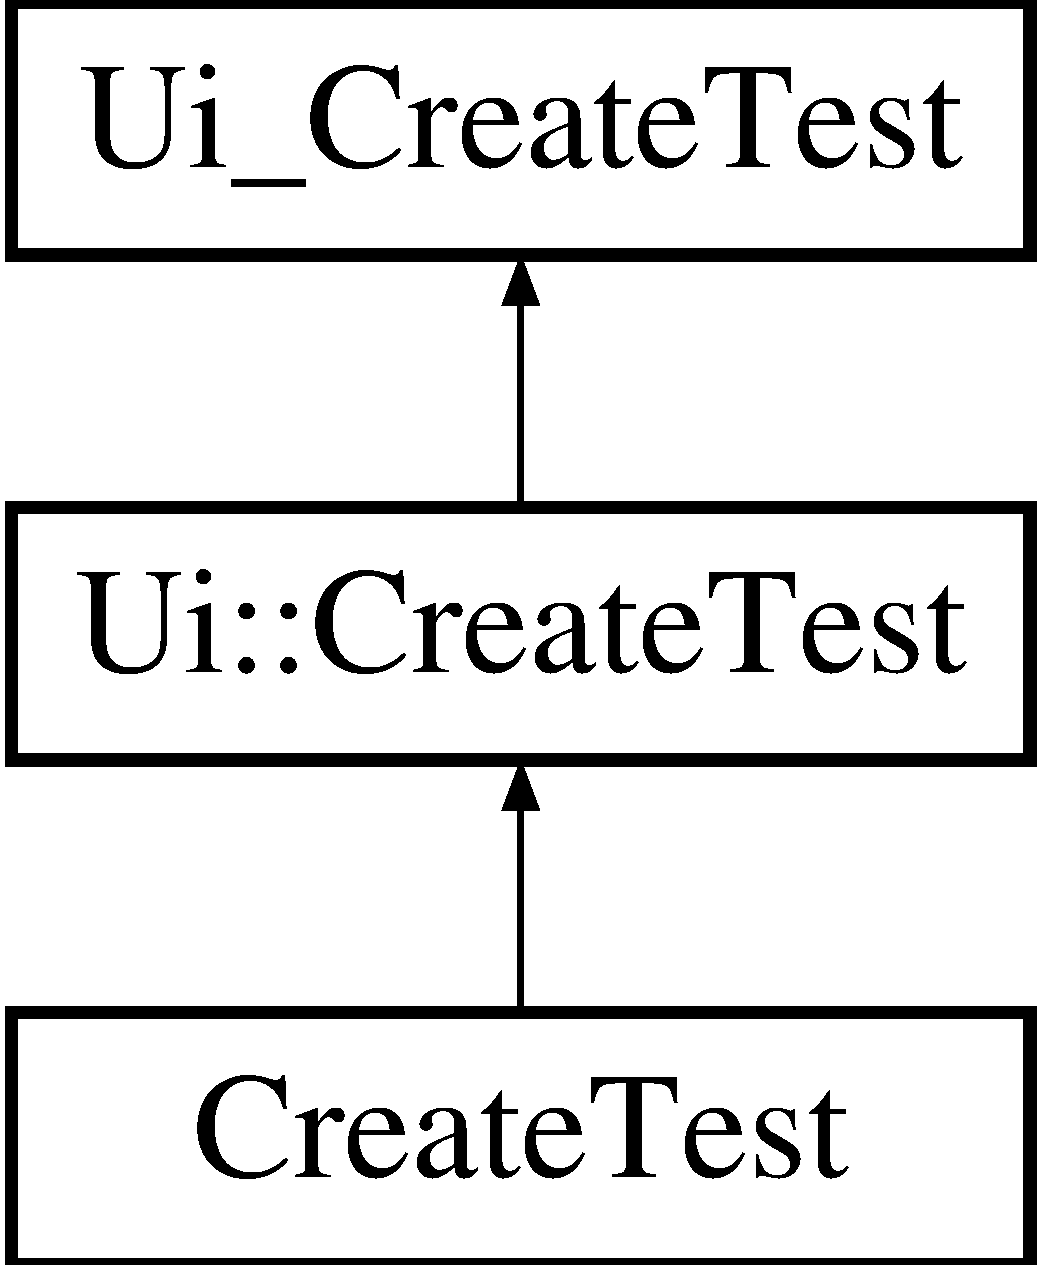
\includegraphics[height=3.000000cm]{class_ui_1_1_create_test}
\end{center}
\end{figure}
\subsection*{Additional Inherited Members}


The documentation for this class was generated from the following file\-:\begin{DoxyCompactItemize}
\item 
Projekt\-Z\-P\-R/\-Generated\-Files/{\bf ui\-\_\-createtest.\-h}\end{DoxyCompactItemize}

\section{Database\-Sqlite Class Reference}
\label{class_database_sqlite}\index{Database\-Sqlite@{Database\-Sqlite}}


{\ttfamily \#include $<$Database\-Sqlite.\-h$>$}

\subsection*{Public Member Functions}
\begin{DoxyCompactItemize}
\item 
{\bf Database\-Sqlite} (void)
\item 
{\bf $\sim$\-Database\-Sqlite} (void)
\end{DoxyCompactItemize}


\subsection{Constructor \& Destructor Documentation}
\index{Database\-Sqlite@{Database\-Sqlite}!Database\-Sqlite@{Database\-Sqlite}}
\index{Database\-Sqlite@{Database\-Sqlite}!DatabaseSqlite@{Database\-Sqlite}}
\subsubsection[{Database\-Sqlite}]{\setlength{\rightskip}{0pt plus 5cm}Database\-Sqlite\-::\-Database\-Sqlite (
\begin{DoxyParamCaption}
\item[{void}]{}
\end{DoxyParamCaption}
)}\label{class_database_sqlite_a601192011e6a7046727195b2d4c73a1a}
\index{Database\-Sqlite@{Database\-Sqlite}!$\sim$\-Database\-Sqlite@{$\sim$\-Database\-Sqlite}}
\index{$\sim$\-Database\-Sqlite@{$\sim$\-Database\-Sqlite}!DatabaseSqlite@{Database\-Sqlite}}
\subsubsection[{$\sim$\-Database\-Sqlite}]{\setlength{\rightskip}{0pt plus 5cm}Database\-Sqlite\-::$\sim$\-Database\-Sqlite (
\begin{DoxyParamCaption}
\item[{void}]{}
\end{DoxyParamCaption}
)}\label{class_database_sqlite_a16e8b8bae860f4d4402c21dd380d10f7}


The documentation for this class was generated from the following files\-:\begin{DoxyCompactItemize}
\item 
Projekt\-Z\-P\-R/{\bf Database\-Sqlite.\-h}\item 
Projekt\-Z\-P\-R/{\bf Database\-Sqlite.\-cpp}\end{DoxyCompactItemize}

\section{Deck Class Reference}
\label{class_deck}\index{Deck@{Deck}}


{\ttfamily \#include $<$deck.\-h$>$}

\subsection*{Public Member Functions}
\begin{DoxyCompactItemize}
\item 
{\bf Deck} ()
\item 
{\bf Deck} (Q\-String filename)
\begin{DoxyCompactList}\small\item\em constructor with file which is loaded \end{DoxyCompactList}\item 
vector$<$ {\bf P\-Qcard} $>$ {\bf get\-Question\-Card\-Vector} ()
\begin{DoxyCompactList}\small\item\em function to get vector of P\-Qcard \end{DoxyCompactList}\item 
{\bf $\sim$\-Deck} ()
\item 
{\footnotesize template$<$class Archive $>$ }\\void {\bf save} (Archive \&ar, const unsigned int version) const 
\item 
{\footnotesize template$<$class Archive $>$ }\\void {\bf load} (Archive \&ar, const unsigned int version)
\end{DoxyCompactItemize}
\subsection*{Public Attributes}
\begin{DoxyCompactItemize}
\item 
vector$<$ {\bf P\-Qcard} $>$ {\bf vector\-P\-Q}
\begin{DoxyCompactList}\small\item\em vector of smart pointers to \doxyref{Question\-Card}{p.}{class_question_card} objects \end{DoxyCompactList}\item 
int {\bf a}
\end{DoxyCompactItemize}
\subsection*{Friends}
\begin{DoxyCompactItemize}
\item 
class {\bf boost\-::serialization\-::access}
\end{DoxyCompactItemize}


\subsection{Detailed Description}
Class represents collection of questions and answers which are showed after users action. (Press apropriate button). Class in its constructor loads from xml file all information. \begin{DoxyAuthor}{Author}
Piotr Malecki \& Michal Daniluk 
\end{DoxyAuthor}


\subsection{Constructor \& Destructor Documentation}
\index{Deck@{Deck}!Deck@{Deck}}
\index{Deck@{Deck}!Deck@{Deck}}
\subsubsection[{Deck}]{\setlength{\rightskip}{0pt plus 5cm}Deck\-::\-Deck (
\begin{DoxyParamCaption}
{}
\end{DoxyParamCaption}
)}\label{class_deck_a57ae1cb4ac6fd61c249cefb2db85eb99}
\index{Deck@{Deck}!Deck@{Deck}}
\index{Deck@{Deck}!Deck@{Deck}}
\subsubsection[{Deck}]{\setlength{\rightskip}{0pt plus 5cm}Deck\-::\-Deck (
\begin{DoxyParamCaption}
\item[{Q\-String}]{filename}
\end{DoxyParamCaption}
)}\label{class_deck_a2de005a2b038321987776b98f754f032}


constructor with file which is loaded 

\index{Deck@{Deck}!$\sim$\-Deck@{$\sim$\-Deck}}
\index{$\sim$\-Deck@{$\sim$\-Deck}!Deck@{Deck}}
\subsubsection[{$\sim$\-Deck}]{\setlength{\rightskip}{0pt plus 5cm}Deck\-::$\sim$\-Deck (
\begin{DoxyParamCaption}
{}
\end{DoxyParamCaption}
)}\label{class_deck_a7d1331cc558c302fdf44e5ae8aae1a95}


\subsection{Member Function Documentation}
\index{Deck@{Deck}!get\-Question\-Card\-Vector@{get\-Question\-Card\-Vector}}
\index{get\-Question\-Card\-Vector@{get\-Question\-Card\-Vector}!Deck@{Deck}}
\subsubsection[{get\-Question\-Card\-Vector}]{\setlength{\rightskip}{0pt plus 5cm}vector$<${\bf P\-Qcard}$>$ Deck\-::get\-Question\-Card\-Vector (
\begin{DoxyParamCaption}
{}
\end{DoxyParamCaption}
)\hspace{0.3cm}{\ttfamily [inline]}}\label{class_deck_a31471a9f843cbd3467688c94748cd70b}


function to get vector of P\-Qcard 

\index{Deck@{Deck}!load@{load}}
\index{load@{load}!Deck@{Deck}}
\subsubsection[{load}]{\setlength{\rightskip}{0pt plus 5cm}template$<$class Archive $>$ void Deck\-::load (
\begin{DoxyParamCaption}
\item[{Archive \&}]{ar, }
\item[{const unsigned int}]{version}
\end{DoxyParamCaption}
)\hspace{0.3cm}{\ttfamily [inline]}}\label{class_deck_a5398698219babba24a524b8ee1bd138b}
\index{Deck@{Deck}!save@{save}}
\index{save@{save}!Deck@{Deck}}
\subsubsection[{save}]{\setlength{\rightskip}{0pt plus 5cm}template$<$class Archive $>$ void Deck\-::save (
\begin{DoxyParamCaption}
\item[{Archive \&}]{ar, }
\item[{const unsigned int}]{version}
\end{DoxyParamCaption}
) const\hspace{0.3cm}{\ttfamily [inline]}}\label{class_deck_a396b0f975aeb9eff075719ac6e99f83d}


\subsection{Friends And Related Function Documentation}
\index{Deck@{Deck}!boost\-::serialization\-::access@{boost\-::serialization\-::access}}
\index{boost\-::serialization\-::access@{boost\-::serialization\-::access}!Deck@{Deck}}
\subsubsection[{boost\-::serialization\-::access}]{\setlength{\rightskip}{0pt plus 5cm}friend class boost\-::serialization\-::access\hspace{0.3cm}{\ttfamily [friend]}}\label{class_deck_ac98d07dd8f7b70e16ccb9a01abf56b9c}


\subsection{Member Data Documentation}
\index{Deck@{Deck}!a@{a}}
\index{a@{a}!Deck@{Deck}}
\subsubsection[{a}]{\setlength{\rightskip}{0pt plus 5cm}int Deck\-::a}\label{class_deck_a91fe9068713c685e8b8a4d308415fc61}
\index{Deck@{Deck}!vector\-P\-Q@{vector\-P\-Q}}
\index{vector\-P\-Q@{vector\-P\-Q}!Deck@{Deck}}
\subsubsection[{vector\-P\-Q}]{\setlength{\rightskip}{0pt plus 5cm}vector$<${\bf P\-Qcard}$>$ Deck\-::vector\-P\-Q}\label{class_deck_a5b0180c72d1a90a495606145beaebfab}


vector of smart pointers to \doxyref{Question\-Card}{p.}{class_question_card} objects 



The documentation for this class was generated from the following files\-:\begin{DoxyCompactItemize}
\item 
Projekt\-Z\-P\-R/{\bf deck.\-h}\item 
Projekt\-Z\-P\-R/{\bf deck.\-cpp}\end{DoxyCompactItemize}

\section{Lack\-File Class Reference}
\label{class_lack_file}\index{Lack\-File@{Lack\-File}}


{\ttfamily \#include $<$Exception.\-h$>$}

Inheritance diagram for Lack\-File\-:\begin{figure}[H]
\begin{center}
\leavevmode
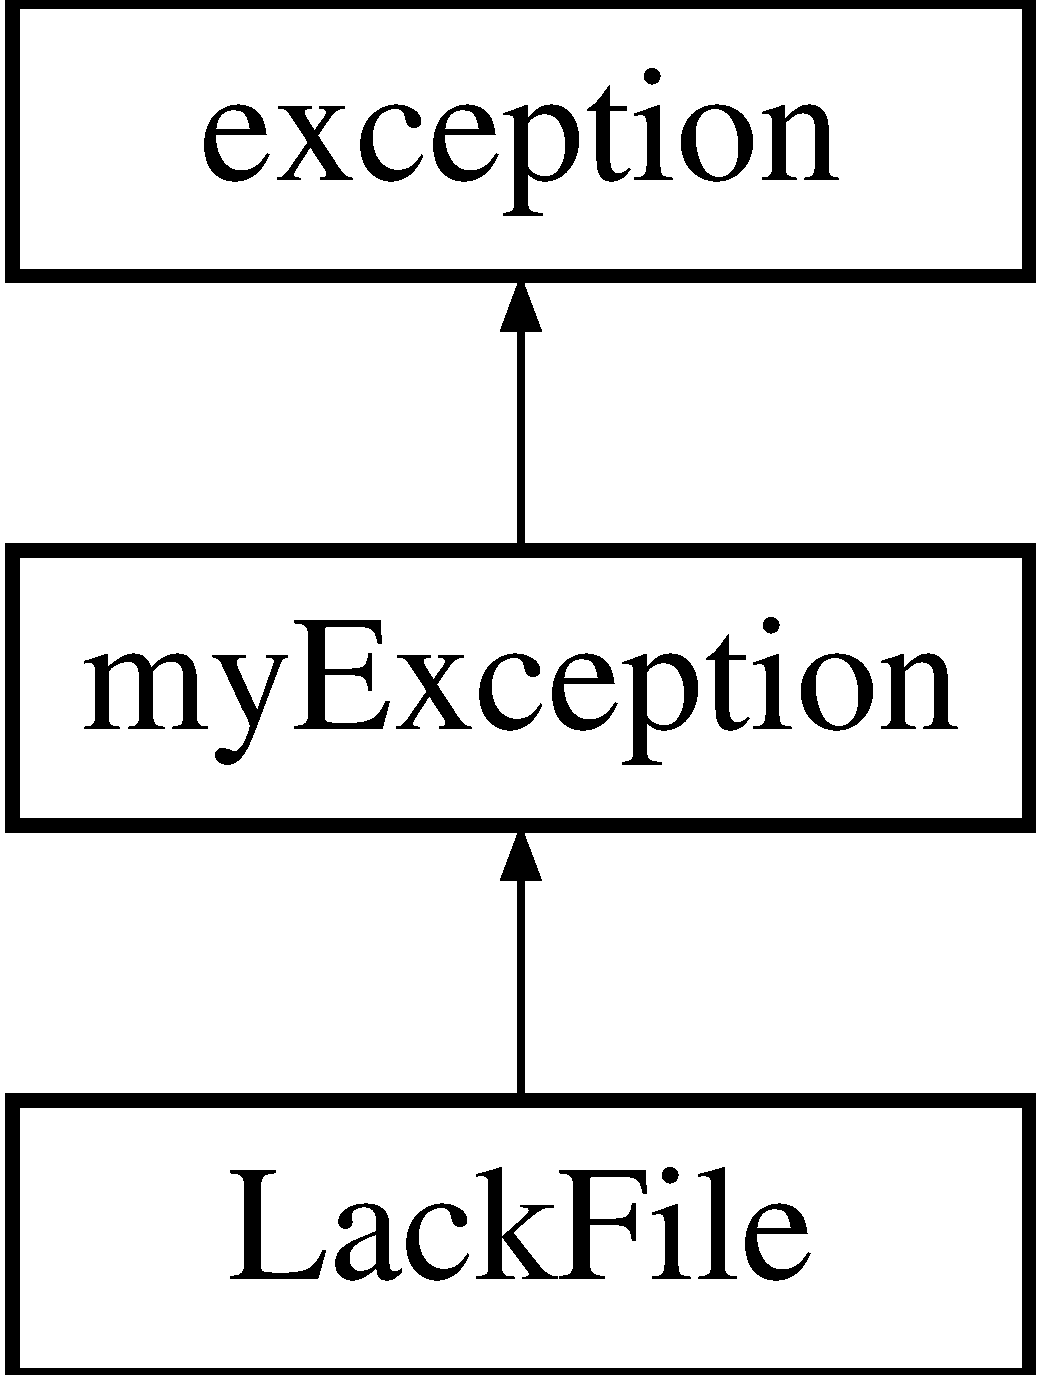
\includegraphics[height=3.000000cm]{class_lack_file}
\end{center}
\end{figure}
\subsection*{Public Member Functions}
\begin{DoxyCompactItemize}
\item 
{\bf Lack\-File} (const string message)
\item 
{\bf $\sim$\-Lack\-File} ()  throw ()
\end{DoxyCompactItemize}


\subsection{Constructor \& Destructor Documentation}
\index{Lack\-File@{Lack\-File}!Lack\-File@{Lack\-File}}
\index{Lack\-File@{Lack\-File}!LackFile@{Lack\-File}}
\subsubsection[{Lack\-File}]{\setlength{\rightskip}{0pt plus 5cm}Lack\-File\-::\-Lack\-File (
\begin{DoxyParamCaption}
\item[{const string}]{message}
\end{DoxyParamCaption}
)\hspace{0.3cm}{\ttfamily [inline]}}\label{class_lack_file_a13aaeae8abf44b972b314904c84cb691}
\index{Lack\-File@{Lack\-File}!$\sim$\-Lack\-File@{$\sim$\-Lack\-File}}
\index{$\sim$\-Lack\-File@{$\sim$\-Lack\-File}!LackFile@{Lack\-File}}
\subsubsection[{$\sim$\-Lack\-File}]{\setlength{\rightskip}{0pt plus 5cm}Lack\-File\-::$\sim$\-Lack\-File (
\begin{DoxyParamCaption}
{}
\end{DoxyParamCaption}
)  throw ()\hspace{0.3cm}{\ttfamily [inline]}}\label{class_lack_file_a44c3b695027d98518946cc470f44a4eb}


The documentation for this class was generated from the following file\-:\begin{DoxyCompactItemize}
\item 
Projekt\-Z\-P\-R/{\bf Exception.\-h}\end{DoxyCompactItemize}

\section{Ui\-:\-:main\-Window Class Reference}
\label{class_ui_1_1main_window}\index{Ui\-::main\-Window@{Ui\-::main\-Window}}


{\ttfamily \#include $<$ui\-\_\-projektzpr.\-h$>$}

Inheritance diagram for Ui\-:\-:main\-Window\-:\begin{figure}[H]
\begin{center}
\leavevmode
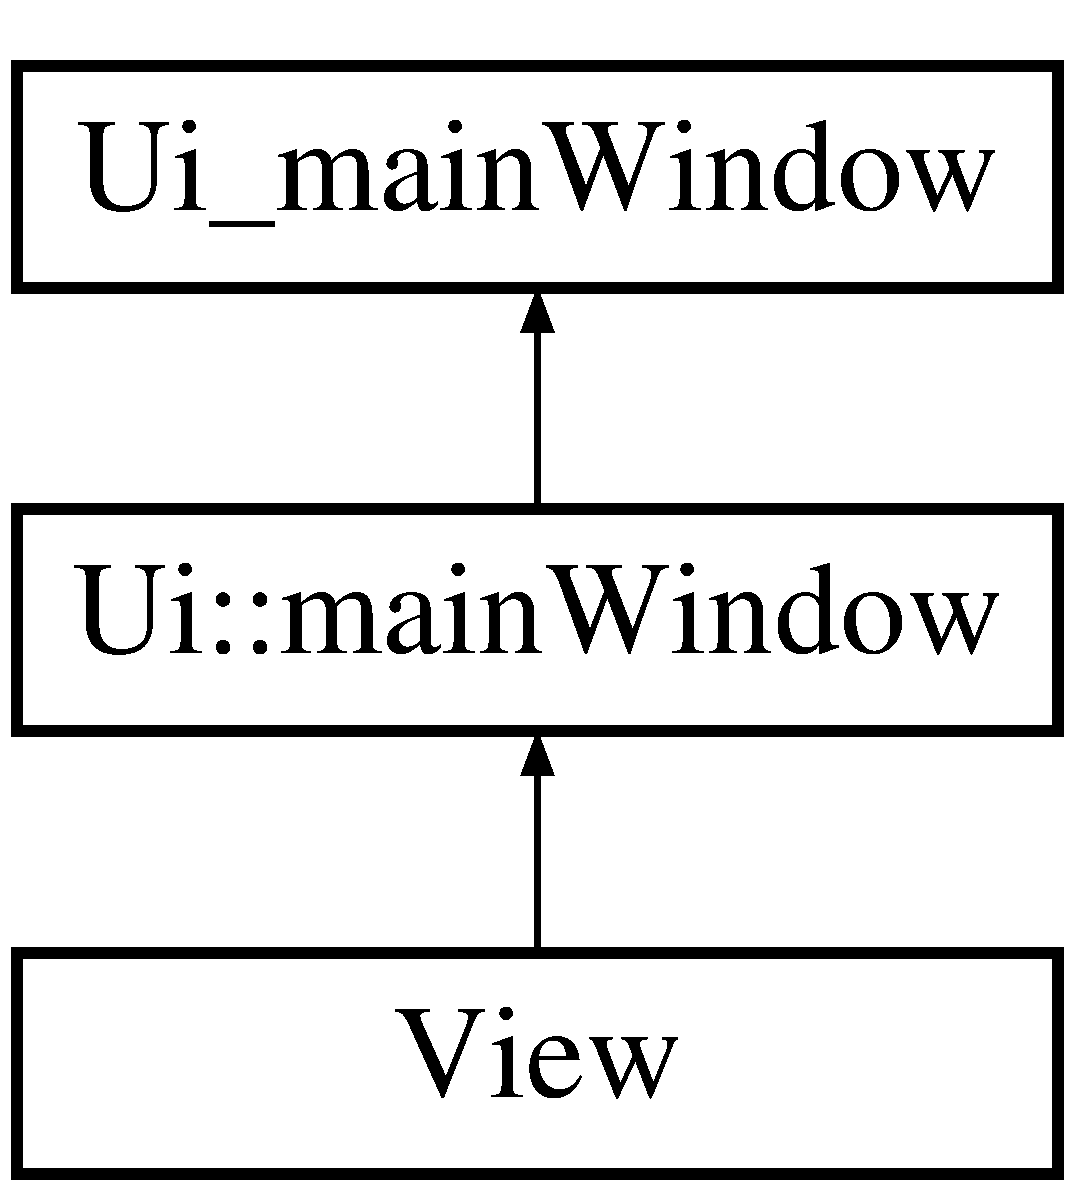
\includegraphics[height=3.000000cm]{class_ui_1_1main_window}
\end{center}
\end{figure}
\subsection*{Additional Inherited Members}


The documentation for this class was generated from the following file\-:\begin{DoxyCompactItemize}
\item 
Projekt\-Z\-P\-R/\-Generated\-Files/{\bf ui\-\_\-projektzpr.\-h}\end{DoxyCompactItemize}

\section{Mark Class Reference}
\label{class_mark}\index{Mark@{Mark}}


{\ttfamily \#include $<$mark.\-h$>$}

\subsection*{Public Member Functions}
\begin{DoxyCompactItemize}
\item 
{\bf Mark} (void)
\item 
{\bf $\sim$\-Mark} (void)
\item 
void {\bf compute\-For\-Open} (int type, std\-::string user, std\-::string correct)
\item 
void {\bf compute\-For\-Close} (int type, std\-::vector$<$ bool $>$ user, std\-::vector$<$ bool $>$ correct)
\item 
int {\bf get\-Value} ()
\end{DoxyCompactItemize}
\subsection*{Private Attributes}
\begin{DoxyCompactItemize}
\item 
int {\bf value\-\_\-}
\end{DoxyCompactItemize}


\subsection{Detailed Description}
Class represents logic of computing mark \begin{DoxyAuthor}{Author}
Piotr Maleci \& Michal Daniluk 
\end{DoxyAuthor}


\subsection{Constructor \& Destructor Documentation}
\index{Mark@{Mark}!Mark@{Mark}}
\index{Mark@{Mark}!Mark@{Mark}}
\subsubsection[{Mark}]{\setlength{\rightskip}{0pt plus 5cm}Mark\-::\-Mark (
\begin{DoxyParamCaption}
\item[{void}]{}
\end{DoxyParamCaption}
)}\label{class_mark_a4ab4671ce05ed543bbaa900e5cd2b00c}
\index{Mark@{Mark}!$\sim$\-Mark@{$\sim$\-Mark}}
\index{$\sim$\-Mark@{$\sim$\-Mark}!Mark@{Mark}}
\subsubsection[{$\sim$\-Mark}]{\setlength{\rightskip}{0pt plus 5cm}Mark\-::$\sim$\-Mark (
\begin{DoxyParamCaption}
\item[{void}]{}
\end{DoxyParamCaption}
)}\label{class_mark_a23678bd0fc1615d061c912209bb76c29}


\subsection{Member Function Documentation}
\index{Mark@{Mark}!compute\-For\-Close@{compute\-For\-Close}}
\index{compute\-For\-Close@{compute\-For\-Close}!Mark@{Mark}}
\subsubsection[{compute\-For\-Close}]{\setlength{\rightskip}{0pt plus 5cm}void Mark\-::compute\-For\-Close (
\begin{DoxyParamCaption}
\item[{int}]{type, }
\item[{std\-::vector$<$ bool $>$}]{user, }
\item[{std\-::vector$<$ bool $>$}]{correct}
\end{DoxyParamCaption}
)}\label{class_mark_ab888fa2a2c3c872cd1b662483e71db01}
\index{Mark@{Mark}!compute\-For\-Open@{compute\-For\-Open}}
\index{compute\-For\-Open@{compute\-For\-Open}!Mark@{Mark}}
\subsubsection[{compute\-For\-Open}]{\setlength{\rightskip}{0pt plus 5cm}void Mark\-::compute\-For\-Open (
\begin{DoxyParamCaption}
\item[{int}]{type, }
\item[{std\-::string}]{user, }
\item[{std\-::string}]{correct}
\end{DoxyParamCaption}
)}\label{class_mark_aa2052d79a782d89f401906adc5862c6a}
\index{Mark@{Mark}!get\-Value@{get\-Value}}
\index{get\-Value@{get\-Value}!Mark@{Mark}}
\subsubsection[{get\-Value}]{\setlength{\rightskip}{0pt plus 5cm}int Mark\-::get\-Value (
\begin{DoxyParamCaption}
{}
\end{DoxyParamCaption}
)\hspace{0.3cm}{\ttfamily [inline]}}\label{class_mark_a79379fb40e8acf172b27ca7bed87a881}


\subsection{Member Data Documentation}
\index{Mark@{Mark}!value\-\_\-@{value\-\_\-}}
\index{value\-\_\-@{value\-\_\-}!Mark@{Mark}}
\subsubsection[{value\-\_\-}]{\setlength{\rightskip}{0pt plus 5cm}int Mark\-::value\-\_\-\hspace{0.3cm}{\ttfamily [private]}}\label{class_mark_ae08ef0c88b83b05f010aaad4e974f3f7}


The documentation for this class was generated from the following files\-:\begin{DoxyCompactItemize}
\item 
Projekt\-Z\-P\-R/{\bf mark.\-h}\item 
Projekt\-Z\-P\-R/{\bf mark.\-cpp}\end{DoxyCompactItemize}

\section{Model Class Reference}
\label{class_model}\index{Model@{Model}}


{\ttfamily \#include $<$model.\-h$>$}

\subsection*{Public Member Functions}
\begin{DoxyCompactItemize}
\item 
{\bf Model} ()
\item 
{\bf $\sim$\-Model} ()
\item 
void {\bf set\-Next} (int id, std\-::string question, std\-::string answer)
\begin{DoxyCompactList}\small\item\em used when set Next is pressed \end{DoxyCompactList}\item 
{\bf Course} $\ast$ {\bf get\-Current\-Course} ()
\begin{DoxyCompactList}\small\item\em to get pointer to course object \end{DoxyCompactList}\item 
{\bf Start} $\ast$ {\bf get\-Current\-Start} ()
\begin{DoxyCompactList}\small\item\em to get pointer to start object \end{DoxyCompactList}\item 
{\bf Mark} $\ast$ {\bf get\-Current\-Mark} ()
\begin{DoxyCompactList}\small\item\em to get pointer to mark object \end{DoxyCompactList}\item 
void {\bf set\-Save\-Course} (std\-::string name\-Of\-File)
\begin{DoxyCompactList}\small\item\em to save course \end{DoxyCompactList}\item 
void {\bf set\-List\-Of\-Files} ()
\begin{DoxyCompactList}\small\item\em used to set list of files \end{DoxyCompactList}\item 
void {\bf set\-Choose\-Course} (std\-::string course, bool flag)
\begin{DoxyCompactList}\small\item\em used to choose course \end{DoxyCompactList}\item 
void {\bf delete\-Choose\-Course} (std\-::string course)
\begin{DoxyCompactList}\small\item\em used when delete clicked \end{DoxyCompactList}\item 
void {\bf end\-Course\-Action} (std\-::vector$<$ int $>$, std\-::string)
\begin{DoxyCompactList}\small\item\em when end clicked \end{DoxyCompactList}\item 
void {\bf compute\-Open\-Mark} (int type, std\-::string user, std\-::string correct)
\begin{DoxyCompactList}\small\item\em used to count mark for open questions \end{DoxyCompactList}\item 
void {\bf compute\-Close\-Mark} (int type, vector$<$ bool $>$ user, vector$<$ bool $>$ correct)
\begin{DoxyCompactList}\small\item\em used to count mark for close questions \end{DoxyCompactList}\item 
void {\bf set\-Choose\-Course\-Continue} (std\-::string name)
\begin{DoxyCompactList}\small\item\em used when continue clicked \end{DoxyCompactList}\end{DoxyCompactItemize}
\subsection*{Private Attributes}
\begin{DoxyCompactItemize}
\item 
{\bf Course} $\ast$ {\bf current\-Course}
\item 
{\bf Start} $\ast$ {\bf start}
\item 
{\bf Mark} $\ast$ {\bf mark}
\item 
{\bf Deck} $\ast$ {\bf deck}
\end{DoxyCompactItemize}


\subsection{Detailed Description}
Class represents \doxyref{Model}{p.}{class_model} in M\-V\-C. \begin{DoxyAuthor}{Author}
Piotr Maleci \& Michal Daniluk 
\end{DoxyAuthor}


\subsection{Constructor \& Destructor Documentation}
\index{Model@{Model}!Model@{Model}}
\index{Model@{Model}!Model@{Model}}
\subsubsection[{Model}]{\setlength{\rightskip}{0pt plus 5cm}Model\-::\-Model (
\begin{DoxyParamCaption}
{}
\end{DoxyParamCaption}
)}\label{class_model_ae3b375de5f6df4faf74a95d64748e048}
\index{Model@{Model}!$\sim$\-Model@{$\sim$\-Model}}
\index{$\sim$\-Model@{$\sim$\-Model}!Model@{Model}}
\subsubsection[{$\sim$\-Model}]{\setlength{\rightskip}{0pt plus 5cm}Model\-::$\sim$\-Model (
\begin{DoxyParamCaption}
{}
\end{DoxyParamCaption}
)}\label{class_model_ad6ebd2062a0b823db841a0b88baac4c0}


\subsection{Member Function Documentation}
\index{Model@{Model}!compute\-Close\-Mark@{compute\-Close\-Mark}}
\index{compute\-Close\-Mark@{compute\-Close\-Mark}!Model@{Model}}
\subsubsection[{compute\-Close\-Mark}]{\setlength{\rightskip}{0pt plus 5cm}void Model\-::compute\-Close\-Mark (
\begin{DoxyParamCaption}
\item[{int}]{type, }
\item[{vector$<$ bool $>$}]{user, }
\item[{vector$<$ bool $>$}]{correct}
\end{DoxyParamCaption}
)}\label{class_model_a96c4b148a2824746ae1959abde9e14e1}


used to count mark for close questions 

\index{Model@{Model}!compute\-Open\-Mark@{compute\-Open\-Mark}}
\index{compute\-Open\-Mark@{compute\-Open\-Mark}!Model@{Model}}
\subsubsection[{compute\-Open\-Mark}]{\setlength{\rightskip}{0pt plus 5cm}void Model\-::compute\-Open\-Mark (
\begin{DoxyParamCaption}
\item[{int}]{type, }
\item[{std\-::string}]{user, }
\item[{std\-::string}]{correct}
\end{DoxyParamCaption}
)}\label{class_model_ab99155ffc02c15a39655def5b3cad3a7}


used to count mark for open questions 

\index{Model@{Model}!delete\-Choose\-Course@{delete\-Choose\-Course}}
\index{delete\-Choose\-Course@{delete\-Choose\-Course}!Model@{Model}}
\subsubsection[{delete\-Choose\-Course}]{\setlength{\rightskip}{0pt plus 5cm}void Model\-::delete\-Choose\-Course (
\begin{DoxyParamCaption}
\item[{std\-::string}]{course}
\end{DoxyParamCaption}
)}\label{class_model_a64496c92b37be0ba6f7b1a21dc42c40f}


used when delete clicked 

\index{Model@{Model}!end\-Course\-Action@{end\-Course\-Action}}
\index{end\-Course\-Action@{end\-Course\-Action}!Model@{Model}}
\subsubsection[{end\-Course\-Action}]{\setlength{\rightskip}{0pt plus 5cm}void Model\-::end\-Course\-Action (
\begin{DoxyParamCaption}
\item[{std\-::vector$<$ int $>$}]{answers\-Judged, }
\item[{std\-::string}]{course\-Name}
\end{DoxyParamCaption}
)}\label{class_model_a1ec87d48fb374790148b0ef6d9e4aad5}


when end clicked 

\index{Model@{Model}!get\-Current\-Course@{get\-Current\-Course}}
\index{get\-Current\-Course@{get\-Current\-Course}!Model@{Model}}
\subsubsection[{get\-Current\-Course}]{\setlength{\rightskip}{0pt plus 5cm}{\bf Course}$\ast$ Model\-::get\-Current\-Course (
\begin{DoxyParamCaption}
{}
\end{DoxyParamCaption}
)\hspace{0.3cm}{\ttfamily [inline]}}\label{class_model_a3213aa4c9b312267ebaca0e8848bc09f}


to get pointer to course object 

\index{Model@{Model}!get\-Current\-Mark@{get\-Current\-Mark}}
\index{get\-Current\-Mark@{get\-Current\-Mark}!Model@{Model}}
\subsubsection[{get\-Current\-Mark}]{\setlength{\rightskip}{0pt plus 5cm}{\bf Mark}$\ast$ Model\-::get\-Current\-Mark (
\begin{DoxyParamCaption}
{}
\end{DoxyParamCaption}
)\hspace{0.3cm}{\ttfamily [inline]}}\label{class_model_ab1828bd7b78669a7fb9efcaeedbfab23}


to get pointer to mark object 

\index{Model@{Model}!get\-Current\-Start@{get\-Current\-Start}}
\index{get\-Current\-Start@{get\-Current\-Start}!Model@{Model}}
\subsubsection[{get\-Current\-Start}]{\setlength{\rightskip}{0pt plus 5cm}{\bf Start}$\ast$ Model\-::get\-Current\-Start (
\begin{DoxyParamCaption}
{}
\end{DoxyParamCaption}
)\hspace{0.3cm}{\ttfamily [inline]}}\label{class_model_aaaf471e62a4d441e4cc02ba9e4230ecd}


to get pointer to start object 

\index{Model@{Model}!set\-Choose\-Course@{set\-Choose\-Course}}
\index{set\-Choose\-Course@{set\-Choose\-Course}!Model@{Model}}
\subsubsection[{set\-Choose\-Course}]{\setlength{\rightskip}{0pt plus 5cm}void Model\-::set\-Choose\-Course (
\begin{DoxyParamCaption}
\item[{std\-::string}]{course, }
\item[{bool}]{flag}
\end{DoxyParamCaption}
)}\label{class_model_a70a651bda1c27902bff97d331b03fc48}


used to choose course 

\index{Model@{Model}!set\-Choose\-Course\-Continue@{set\-Choose\-Course\-Continue}}
\index{set\-Choose\-Course\-Continue@{set\-Choose\-Course\-Continue}!Model@{Model}}
\subsubsection[{set\-Choose\-Course\-Continue}]{\setlength{\rightskip}{0pt plus 5cm}void Model\-::set\-Choose\-Course\-Continue (
\begin{DoxyParamCaption}
\item[{std\-::string}]{name}
\end{DoxyParamCaption}
)}\label{class_model_a1821aed1f84fcedff1d0396ef197d53e}


used when continue clicked 

\index{Model@{Model}!set\-List\-Of\-Files@{set\-List\-Of\-Files}}
\index{set\-List\-Of\-Files@{set\-List\-Of\-Files}!Model@{Model}}
\subsubsection[{set\-List\-Of\-Files}]{\setlength{\rightskip}{0pt plus 5cm}void Model\-::set\-List\-Of\-Files (
\begin{DoxyParamCaption}
{}
\end{DoxyParamCaption}
)}\label{class_model_a937d7c21c027c61ab6db7b146fb66518}


used to set list of files 

\index{Model@{Model}!set\-Next@{set\-Next}}
\index{set\-Next@{set\-Next}!Model@{Model}}
\subsubsection[{set\-Next}]{\setlength{\rightskip}{0pt plus 5cm}void Model\-::set\-Next (
\begin{DoxyParamCaption}
\item[{int}]{id, }
\item[{std\-::string}]{question, }
\item[{std\-::string}]{answer}
\end{DoxyParamCaption}
)}\label{class_model_a31d4f8b7432120e4e2524d3a69e6ff54}


used when set Next is pressed 

\index{Model@{Model}!set\-Save\-Course@{set\-Save\-Course}}
\index{set\-Save\-Course@{set\-Save\-Course}!Model@{Model}}
\subsubsection[{set\-Save\-Course}]{\setlength{\rightskip}{0pt plus 5cm}void Model\-::set\-Save\-Course (
\begin{DoxyParamCaption}
\item[{std\-::string}]{name\-Of\-File}
\end{DoxyParamCaption}
)}\label{class_model_a1a491166f5a11220c7f0f1b0e84b8123}


to save course 



\subsection{Member Data Documentation}
\index{Model@{Model}!current\-Course@{current\-Course}}
\index{current\-Course@{current\-Course}!Model@{Model}}
\subsubsection[{current\-Course}]{\setlength{\rightskip}{0pt plus 5cm}{\bf Course}$\ast$ Model\-::current\-Course\hspace{0.3cm}{\ttfamily [private]}}\label{class_model_ac3b91a3ed954e175ae34ea2308950efe}
\index{Model@{Model}!deck@{deck}}
\index{deck@{deck}!Model@{Model}}
\subsubsection[{deck}]{\setlength{\rightskip}{0pt plus 5cm}{\bf Deck}$\ast$ Model\-::deck\hspace{0.3cm}{\ttfamily [private]}}\label{class_model_af4659340fc1cd97928ddb3312486c867}
\index{Model@{Model}!mark@{mark}}
\index{mark@{mark}!Model@{Model}}
\subsubsection[{mark}]{\setlength{\rightskip}{0pt plus 5cm}{\bf Mark}$\ast$ Model\-::mark\hspace{0.3cm}{\ttfamily [private]}}\label{class_model_a430b9f920220066900c35ee00dda9418}
\index{Model@{Model}!start@{start}}
\index{start@{start}!Model@{Model}}
\subsubsection[{start}]{\setlength{\rightskip}{0pt plus 5cm}{\bf Start}$\ast$ Model\-::start\hspace{0.3cm}{\ttfamily [private]}}\label{class_model_af1d966b88165e49caf54ce4c4841c534}


The documentation for this class was generated from the following files\-:\begin{DoxyCompactItemize}
\item 
Projekt\-Z\-P\-R/{\bf model.\-h}\item 
Projekt\-Z\-P\-R/{\bf model.\-cpp}\end{DoxyCompactItemize}

\section{my\-Exception Class Reference}
\label{classmy_exception}\index{my\-Exception@{my\-Exception}}


{\ttfamily \#include $<$Exception.\-h$>$}

Inheritance diagram for my\-Exception\-:\begin{figure}[H]
\begin{center}
\leavevmode
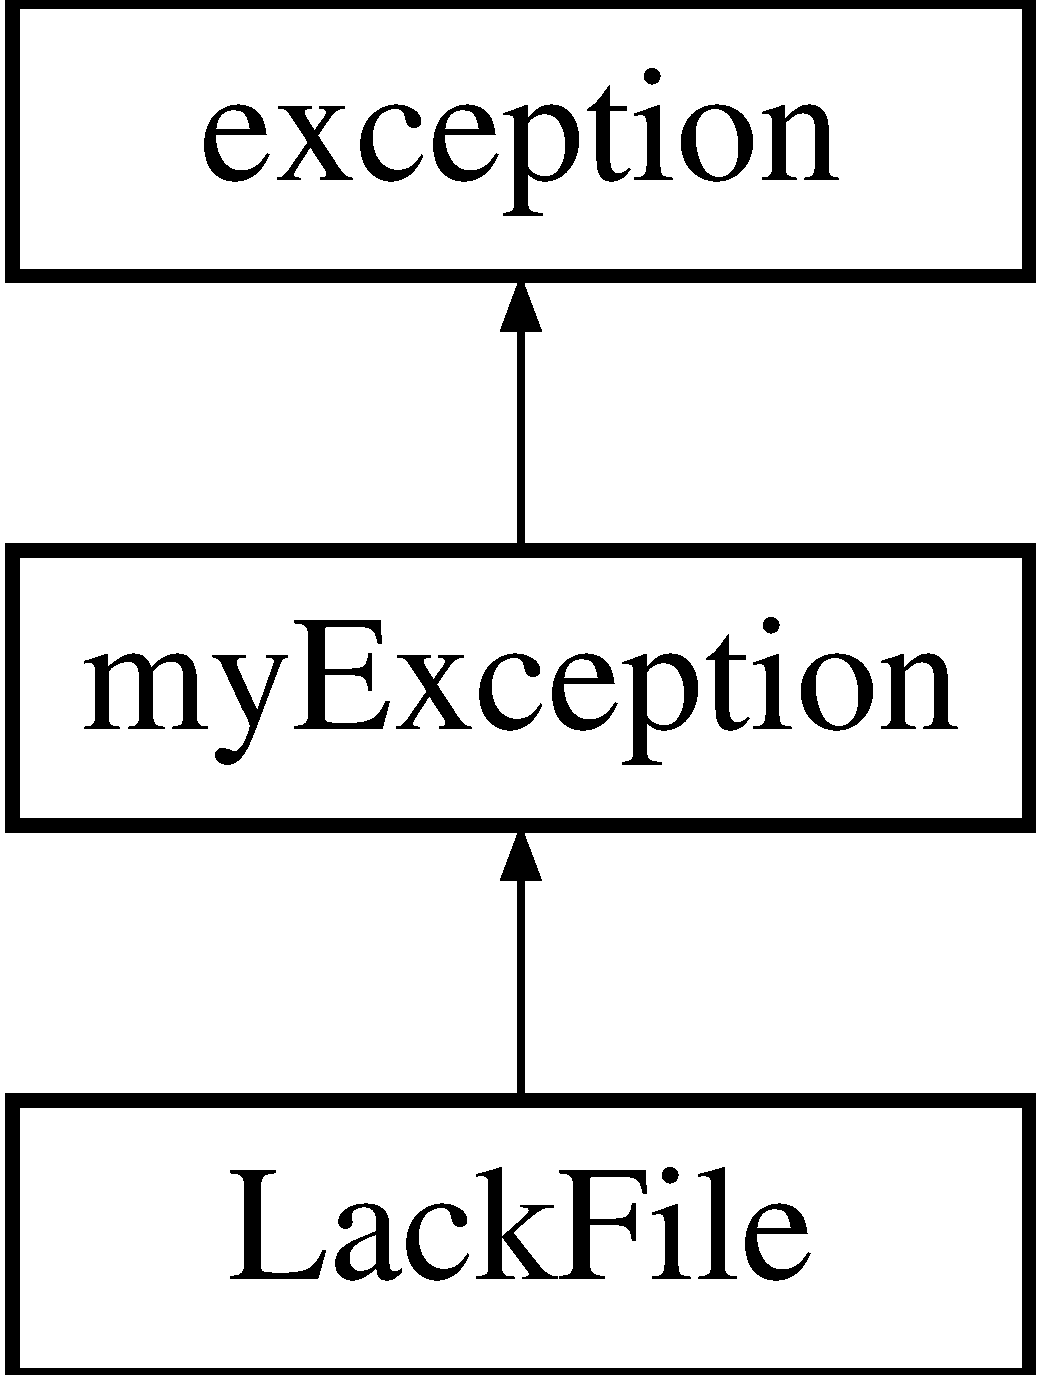
\includegraphics[height=3.000000cm]{classmy_exception}
\end{center}
\end{figure}
\subsection*{Public Member Functions}
\begin{DoxyCompactItemize}
\item 
{\bf my\-Exception} (const string message)
\item 
const string {\bf return\-Message} () const 
\item 
{\bf $\sim$my\-Exception} ()  throw ()
\end{DoxyCompactItemize}
\subsection*{Private Attributes}
\begin{DoxyCompactItemize}
\item 
const string {\bf message\-\_\-}
\end{DoxyCompactItemize}


\subsection{Detailed Description}
Class represents our own Exception \begin{DoxyAuthor}{Author}
Piotr Maleci \& Michal Daniluk 
\end{DoxyAuthor}


\subsection{Constructor \& Destructor Documentation}
\index{my\-Exception@{my\-Exception}!my\-Exception@{my\-Exception}}
\index{my\-Exception@{my\-Exception}!myException@{my\-Exception}}
\subsubsection[{my\-Exception}]{\setlength{\rightskip}{0pt plus 5cm}my\-Exception\-::my\-Exception (
\begin{DoxyParamCaption}
\item[{const string}]{message}
\end{DoxyParamCaption}
)\hspace{0.3cm}{\ttfamily [inline]}}\label{classmy_exception_a8ab341de1fc4e50ea72577766410b1a5}
\index{my\-Exception@{my\-Exception}!$\sim$my\-Exception@{$\sim$my\-Exception}}
\index{$\sim$my\-Exception@{$\sim$my\-Exception}!myException@{my\-Exception}}
\subsubsection[{$\sim$my\-Exception}]{\setlength{\rightskip}{0pt plus 5cm}my\-Exception\-::$\sim$my\-Exception (
\begin{DoxyParamCaption}
{}
\end{DoxyParamCaption}
)  throw ()\hspace{0.3cm}{\ttfamily [inline]}}\label{classmy_exception_a5c7c2fb05755a2eaeb7a64915782f18c}


\subsection{Member Function Documentation}
\index{my\-Exception@{my\-Exception}!return\-Message@{return\-Message}}
\index{return\-Message@{return\-Message}!myException@{my\-Exception}}
\subsubsection[{return\-Message}]{\setlength{\rightskip}{0pt plus 5cm}const string my\-Exception\-::return\-Message (
\begin{DoxyParamCaption}
{}
\end{DoxyParamCaption}
) const\hspace{0.3cm}{\ttfamily [inline]}}\label{classmy_exception_a8ac33628bc4cdf1d5cb9ec6d080e06d6}


\subsection{Member Data Documentation}
\index{my\-Exception@{my\-Exception}!message\-\_\-@{message\-\_\-}}
\index{message\-\_\-@{message\-\_\-}!myException@{my\-Exception}}
\subsubsection[{message\-\_\-}]{\setlength{\rightskip}{0pt plus 5cm}const string my\-Exception\-::message\-\_\-\hspace{0.3cm}{\ttfamily [private]}}\label{classmy_exception_a4cff8cb0dfe98cee455670a236aa1d60}


The documentation for this class was generated from the following file\-:\begin{DoxyCompactItemize}
\item 
Projekt\-Z\-P\-R/{\bf Exception.\-h}\end{DoxyCompactItemize}

\section{qt\-\_\-meta\-\_\-stringdata\-\_\-\-Controller\-\_\-t Struct Reference}
\label{structqt__meta__stringdata___controller__t}\index{qt\-\_\-meta\-\_\-stringdata\-\_\-\-Controller\-\_\-t@{qt\-\_\-meta\-\_\-stringdata\-\_\-\-Controller\-\_\-t}}
\subsection*{Public Attributes}
\begin{DoxyCompactItemize}
\item 
Q\-Byte\-Array\-Data {\bf data} [37]
\item 
char {\bf stringdata} [502]
\end{DoxyCompactItemize}


\subsection{Member Data Documentation}
\index{qt\-\_\-meta\-\_\-stringdata\-\_\-\-Controller\-\_\-t@{qt\-\_\-meta\-\_\-stringdata\-\_\-\-Controller\-\_\-t}!data@{data}}
\index{data@{data}!qt_meta_stringdata_Controller_t@{qt\-\_\-meta\-\_\-stringdata\-\_\-\-Controller\-\_\-t}}
\subsubsection[{data}]{\setlength{\rightskip}{0pt plus 5cm}Q\-Byte\-Array\-Data qt\-\_\-meta\-\_\-stringdata\-\_\-\-Controller\-\_\-t\-::data}\label{structqt__meta__stringdata___controller__t_a85f61ff9015de00512cc5108f62e86f7}
\index{qt\-\_\-meta\-\_\-stringdata\-\_\-\-Controller\-\_\-t@{qt\-\_\-meta\-\_\-stringdata\-\_\-\-Controller\-\_\-t}!stringdata@{stringdata}}
\index{stringdata@{stringdata}!qt_meta_stringdata_Controller_t@{qt\-\_\-meta\-\_\-stringdata\-\_\-\-Controller\-\_\-t}}
\subsubsection[{stringdata}]{\setlength{\rightskip}{0pt plus 5cm}char qt\-\_\-meta\-\_\-stringdata\-\_\-\-Controller\-\_\-t\-::stringdata}\label{structqt__meta__stringdata___controller__t_aec181748e9af78d66ac11fbc848719c4}


The documentation for this struct was generated from the following files\-:\begin{DoxyCompactItemize}
\item 
Projekt\-Z\-P\-R/\-Generated\-Files/\-Debug/{\bf moc\-\_\-controller.\-cpp}\item 
Projekt\-Z\-P\-R/\-Generated\-Files/\-Release/{\bf moc\-\_\-controller.\-cpp}\item 
Projekt\-Z\-P\-R/\-Generated\-Files/\-Testy\-Z\-P\-R/{\bf moc\-\_\-controller.\-cpp}\item 
Projekt\-Z\-P\-R/\-Generated\-Files/\-Testy\-Z\-P\-R2/{\bf moc\-\_\-controller.\-cpp}\end{DoxyCompactItemize}

\section{qt\-\_\-meta\-\_\-stringdata\-\_\-\-Create\-Test\-\_\-t Struct Reference}
\label{structqt__meta__stringdata___create_test__t}\index{qt\-\_\-meta\-\_\-stringdata\-\_\-\-Create\-Test\-\_\-t@{qt\-\_\-meta\-\_\-stringdata\-\_\-\-Create\-Test\-\_\-t}}
\subsection*{Public Attributes}
\begin{DoxyCompactItemize}
\item 
Q\-Byte\-Array\-Data {\bf data} [20]
\item 
char {\bf stringdata} [224]
\end{DoxyCompactItemize}


\subsection{Member Data Documentation}
\index{qt\-\_\-meta\-\_\-stringdata\-\_\-\-Create\-Test\-\_\-t@{qt\-\_\-meta\-\_\-stringdata\-\_\-\-Create\-Test\-\_\-t}!data@{data}}
\index{data@{data}!qt_meta_stringdata_CreateTest_t@{qt\-\_\-meta\-\_\-stringdata\-\_\-\-Create\-Test\-\_\-t}}
\subsubsection[{data}]{\setlength{\rightskip}{0pt plus 5cm}Q\-Byte\-Array\-Data qt\-\_\-meta\-\_\-stringdata\-\_\-\-Create\-Test\-\_\-t\-::data}\label{structqt__meta__stringdata___create_test__t_a8f26e164cb2f52d822837d3f0549c30f}
\index{qt\-\_\-meta\-\_\-stringdata\-\_\-\-Create\-Test\-\_\-t@{qt\-\_\-meta\-\_\-stringdata\-\_\-\-Create\-Test\-\_\-t}!stringdata@{stringdata}}
\index{stringdata@{stringdata}!qt_meta_stringdata_CreateTest_t@{qt\-\_\-meta\-\_\-stringdata\-\_\-\-Create\-Test\-\_\-t}}
\subsubsection[{stringdata}]{\setlength{\rightskip}{0pt plus 5cm}char qt\-\_\-meta\-\_\-stringdata\-\_\-\-Create\-Test\-\_\-t\-::stringdata}\label{structqt__meta__stringdata___create_test__t_ae14c85848e292409260ba5e36cf19682}


The documentation for this struct was generated from the following files\-:\begin{DoxyCompactItemize}
\item 
Projekt\-Z\-P\-R/\-Generated\-Files/\-Debug/{\bf moc\-\_\-createtest.\-cpp}\item 
Projekt\-Z\-P\-R/\-Generated\-Files/\-Release/{\bf moc\-\_\-createtest.\-cpp}\item 
Projekt\-Z\-P\-R/\-Generated\-Files/\-Testy\-Z\-P\-R/{\bf moc\-\_\-createtest.\-cpp}\item 
Projekt\-Z\-P\-R/\-Generated\-Files/\-Testy\-Z\-P\-R2/{\bf moc\-\_\-createtest.\-cpp}\end{DoxyCompactItemize}

\section{qt\-\_\-meta\-\_\-stringdata\-\_\-\-Schedule\-\_\-t Struct Reference}
\label{structqt__meta__stringdata___schedule__t}\index{qt\-\_\-meta\-\_\-stringdata\-\_\-\-Schedule\-\_\-t@{qt\-\_\-meta\-\_\-stringdata\-\_\-\-Schedule\-\_\-t}}
\subsection*{Public Attributes}
\begin{DoxyCompactItemize}
\item 
Q\-Byte\-Array\-Data {\bf data} [1]
\item 
char {\bf stringdata} [10]
\end{DoxyCompactItemize}


\subsection{Member Data Documentation}
\index{qt\-\_\-meta\-\_\-stringdata\-\_\-\-Schedule\-\_\-t@{qt\-\_\-meta\-\_\-stringdata\-\_\-\-Schedule\-\_\-t}!data@{data}}
\index{data@{data}!qt_meta_stringdata_Schedule_t@{qt\-\_\-meta\-\_\-stringdata\-\_\-\-Schedule\-\_\-t}}
\subsubsection[{data}]{\setlength{\rightskip}{0pt plus 5cm}Q\-Byte\-Array\-Data qt\-\_\-meta\-\_\-stringdata\-\_\-\-Schedule\-\_\-t\-::data}\label{structqt__meta__stringdata___schedule__t_a16b0dc70fb28f1a0b5aa5bbf7256a23c}
\index{qt\-\_\-meta\-\_\-stringdata\-\_\-\-Schedule\-\_\-t@{qt\-\_\-meta\-\_\-stringdata\-\_\-\-Schedule\-\_\-t}!stringdata@{stringdata}}
\index{stringdata@{stringdata}!qt_meta_stringdata_Schedule_t@{qt\-\_\-meta\-\_\-stringdata\-\_\-\-Schedule\-\_\-t}}
\subsubsection[{stringdata}]{\setlength{\rightskip}{0pt plus 5cm}char qt\-\_\-meta\-\_\-stringdata\-\_\-\-Schedule\-\_\-t\-::stringdata}\label{structqt__meta__stringdata___schedule__t_a475fb5f203cd226d733a6e128053d176}


The documentation for this struct was generated from the following files\-:\begin{DoxyCompactItemize}
\item 
Projekt\-Z\-P\-R/\-Generated\-Files/\-Debug/{\bf moc\-\_\-schedule.\-cpp}\item 
Projekt\-Z\-P\-R/\-Generated\-Files/\-Testy\-Z\-P\-R/{\bf moc\-\_\-schedule.\-cpp}\item 
Projekt\-Z\-P\-R/\-Generated\-Files/\-Testy\-Z\-P\-R2/{\bf moc\-\_\-schedule.\-cpp}\end{DoxyCompactItemize}

\section{qt\-\_\-meta\-\_\-stringdata\-\_\-\-Start\-Menu\-\_\-t Struct Reference}
\label{structqt__meta__stringdata___start_menu__t}\index{qt\-\_\-meta\-\_\-stringdata\-\_\-\-Start\-Menu\-\_\-t@{qt\-\_\-meta\-\_\-stringdata\-\_\-\-Start\-Menu\-\_\-t}}
\subsection*{Public Attributes}
\begin{DoxyCompactItemize}
\item 
Q\-Byte\-Array\-Data {\bf data} [15]
\item 
char {\bf stringdata} [220]
\end{DoxyCompactItemize}


\subsection{Member Data Documentation}
\index{qt\-\_\-meta\-\_\-stringdata\-\_\-\-Start\-Menu\-\_\-t@{qt\-\_\-meta\-\_\-stringdata\-\_\-\-Start\-Menu\-\_\-t}!data@{data}}
\index{data@{data}!qt_meta_stringdata_StartMenu_t@{qt\-\_\-meta\-\_\-stringdata\-\_\-\-Start\-Menu\-\_\-t}}
\subsubsection[{data}]{\setlength{\rightskip}{0pt plus 5cm}Q\-Byte\-Array\-Data qt\-\_\-meta\-\_\-stringdata\-\_\-\-Start\-Menu\-\_\-t\-::data}\label{structqt__meta__stringdata___start_menu__t_ae509bf58298e44ba59c1b5460d7b8e7a}
\index{qt\-\_\-meta\-\_\-stringdata\-\_\-\-Start\-Menu\-\_\-t@{qt\-\_\-meta\-\_\-stringdata\-\_\-\-Start\-Menu\-\_\-t}!stringdata@{stringdata}}
\index{stringdata@{stringdata}!qt_meta_stringdata_StartMenu_t@{qt\-\_\-meta\-\_\-stringdata\-\_\-\-Start\-Menu\-\_\-t}}
\subsubsection[{stringdata}]{\setlength{\rightskip}{0pt plus 5cm}char qt\-\_\-meta\-\_\-stringdata\-\_\-\-Start\-Menu\-\_\-t\-::stringdata}\label{structqt__meta__stringdata___start_menu__t_aacde7f105462fe9ea00fe7c49dc06124}


The documentation for this struct was generated from the following files\-:\begin{DoxyCompactItemize}
\item 
Projekt\-Z\-P\-R/\-Generated\-Files/\-Debug/{\bf moc\-\_\-startmenu.\-cpp}\item 
Projekt\-Z\-P\-R/\-Generated\-Files/\-Release/{\bf moc\-\_\-startmenu.\-cpp}\item 
Projekt\-Z\-P\-R/\-Generated\-Files/\-Testy\-Z\-P\-R/{\bf moc\-\_\-startmenu.\-cpp}\item 
Projekt\-Z\-P\-R/\-Generated\-Files/\-Testy\-Z\-P\-R2/{\bf moc\-\_\-startmenu.\-cpp}\end{DoxyCompactItemize}

\section{qt\-\_\-meta\-\_\-stringdata\-\_\-\-Statistic\-\_\-t Struct Reference}
\label{structqt__meta__stringdata___statistic__t}\index{qt\-\_\-meta\-\_\-stringdata\-\_\-\-Statistic\-\_\-t@{qt\-\_\-meta\-\_\-stringdata\-\_\-\-Statistic\-\_\-t}}
\subsection*{Public Attributes}
\begin{DoxyCompactItemize}
\item 
Q\-Byte\-Array\-Data {\bf data} [4]
\item 
char {\bf stringdata} [38]
\end{DoxyCompactItemize}


\subsection{Member Data Documentation}
\index{qt\-\_\-meta\-\_\-stringdata\-\_\-\-Statistic\-\_\-t@{qt\-\_\-meta\-\_\-stringdata\-\_\-\-Statistic\-\_\-t}!data@{data}}
\index{data@{data}!qt_meta_stringdata_Statistic_t@{qt\-\_\-meta\-\_\-stringdata\-\_\-\-Statistic\-\_\-t}}
\subsubsection[{data}]{\setlength{\rightskip}{0pt plus 5cm}Q\-Byte\-Array\-Data qt\-\_\-meta\-\_\-stringdata\-\_\-\-Statistic\-\_\-t\-::data}\label{structqt__meta__stringdata___statistic__t_aacc35c824e5433c6ea03fe785f20801a}
\index{qt\-\_\-meta\-\_\-stringdata\-\_\-\-Statistic\-\_\-t@{qt\-\_\-meta\-\_\-stringdata\-\_\-\-Statistic\-\_\-t}!stringdata@{stringdata}}
\index{stringdata@{stringdata}!qt_meta_stringdata_Statistic_t@{qt\-\_\-meta\-\_\-stringdata\-\_\-\-Statistic\-\_\-t}}
\subsubsection[{stringdata}]{\setlength{\rightskip}{0pt plus 5cm}char qt\-\_\-meta\-\_\-stringdata\-\_\-\-Statistic\-\_\-t\-::stringdata}\label{structqt__meta__stringdata___statistic__t_a91da8553731bcc28473f5274043a107c}


The documentation for this struct was generated from the following files\-:\begin{DoxyCompactItemize}
\item 
Projekt\-Z\-P\-R/\-Generated\-Files/\-Debug/{\bf moc\-\_\-statistic.\-cpp}\item 
Projekt\-Z\-P\-R/\-Generated\-Files/\-Release/{\bf moc\-\_\-statistic.\-cpp}\item 
Projekt\-Z\-P\-R/\-Generated\-Files/\-Testy\-Z\-P\-R/{\bf moc\-\_\-statistic.\-cpp}\item 
Projekt\-Z\-P\-R/\-Generated\-Files/\-Testy\-Z\-P\-R2/{\bf moc\-\_\-statistic.\-cpp}\end{DoxyCompactItemize}

\section{qt\-\_\-meta\-\_\-stringdata\-\_\-\-View\-\_\-t Struct Reference}
\label{structqt__meta__stringdata___view__t}\index{qt\-\_\-meta\-\_\-stringdata\-\_\-\-View\-\_\-t@{qt\-\_\-meta\-\_\-stringdata\-\_\-\-View\-\_\-t}}
\subsection*{Public Attributes}
\begin{DoxyCompactItemize}
\item 
Q\-Byte\-Array\-Data {\bf data} [42]
\item 
char {\bf stringdata} [667]
\end{DoxyCompactItemize}


\subsection{Member Data Documentation}
\index{qt\-\_\-meta\-\_\-stringdata\-\_\-\-View\-\_\-t@{qt\-\_\-meta\-\_\-stringdata\-\_\-\-View\-\_\-t}!data@{data}}
\index{data@{data}!qt_meta_stringdata_View_t@{qt\-\_\-meta\-\_\-stringdata\-\_\-\-View\-\_\-t}}
\subsubsection[{data}]{\setlength{\rightskip}{0pt plus 5cm}Q\-Byte\-Array\-Data qt\-\_\-meta\-\_\-stringdata\-\_\-\-View\-\_\-t\-::data}\label{structqt__meta__stringdata___view__t_a37b74396a22dc946220b5d3ac1a6546d}
\index{qt\-\_\-meta\-\_\-stringdata\-\_\-\-View\-\_\-t@{qt\-\_\-meta\-\_\-stringdata\-\_\-\-View\-\_\-t}!stringdata@{stringdata}}
\index{stringdata@{stringdata}!qt_meta_stringdata_View_t@{qt\-\_\-meta\-\_\-stringdata\-\_\-\-View\-\_\-t}}
\subsubsection[{stringdata}]{\setlength{\rightskip}{0pt plus 5cm}char qt\-\_\-meta\-\_\-stringdata\-\_\-\-View\-\_\-t\-::stringdata}\label{structqt__meta__stringdata___view__t_aa97b67573d1d28bf88f803a713abdd66}


The documentation for this struct was generated from the following files\-:\begin{DoxyCompactItemize}
\item 
Projekt\-Z\-P\-R/\-Generated\-Files/\-Debug/{\bf moc\-\_\-view.\-cpp}\item 
Projekt\-Z\-P\-R/\-Generated\-Files/\-Release/{\bf moc\-\_\-view.\-cpp}\item 
Projekt\-Z\-P\-R/\-Generated\-Files/\-Testy\-Z\-P\-R/{\bf moc\-\_\-view.\-cpp}\item 
Projekt\-Z\-P\-R/\-Generated\-Files/\-Testy\-Z\-P\-R2/{\bf moc\-\_\-view.\-cpp}\end{DoxyCompactItemize}

\section{Question\-Card Class Reference}
\label{class_question_card}\index{Question\-Card@{Question\-Card}}


{\ttfamily \#include $<$questioncard.\-h$>$}

\subsection*{Public Member Functions}
\begin{DoxyCompactItemize}
\item 
{\bf Question\-Card} ()
\item 
{\bf Question\-Card} (const std\-::string question, const std\-::string answer, const int id\-Question, const bool question\-Type)
\item 
{\bf Question\-Card} (const std\-::string question, {\bf Close\-Answer} closeanswer, const int id\-Question, const bool question\-Type)
\item 
boost\-::gregorian\-::date {\bf date\-Of\-Next\-Question} (int mark)
\item 
bool {\bf get\-Question\-Type} ()
\item 
int {\bf get\-Id\-Question} ()
\item 
string {\bf get\-Answer\-Open} ()
\item 
string {\bf get\-Question} ()
\item 
{\bf Close\-Answer} {\bf getclose\-Answer} ()
\item 
boost\-::gregorian\-::date {\bf get\-Next\-Date} ()
\item 
{\bf $\sim$\-Question\-Card} ()
\item 
{\footnotesize template$<$class Archive $>$ }\\void {\bf save} (Archive \&ar, const unsigned int version) const 
\item 
{\footnotesize template$<$class Archive $>$ }\\void {\bf load} (Archive \&ar, const unsigned int version)
\end{DoxyCompactItemize}
\subsection*{Public Attributes}
\begin{DoxyCompactItemize}
\item 
bool {\bf question\-Type\-\_\-}
\item 
int {\bf id\-Question\-\_\-}
\item 
string {\bf answer\-Open\-\_\-}
\item 
string {\bf question\-\_\-}
\item 
{\bf Close\-Answer} {\bf close\-Answer\-\_\-}
\item 
int {\bf how\-\_\-many\-\_\-}
\item 
double {\bf e\-Factor\-\_\-}
\item 
double {\bf interval\-\_\-}
\item 
boost\-::gregorian\-::date {\bf now}
\end{DoxyCompactItemize}
\subsection*{Friends}
\begin{DoxyCompactItemize}
\item 
class {\bf boost\-::serialization\-::access}
\end{DoxyCompactItemize}


\subsection{Detailed Description}
Class which represents logical structure of question, consists all elements of question. Enables setting next date of showing each question. \begin{DoxyAuthor}{Author}
Piotr 
\end{DoxyAuthor}


\subsection{Constructor \& Destructor Documentation}
\index{Question\-Card@{Question\-Card}!Question\-Card@{Question\-Card}}
\index{Question\-Card@{Question\-Card}!QuestionCard@{Question\-Card}}
\subsubsection[{Question\-Card}]{\setlength{\rightskip}{0pt plus 5cm}Question\-Card\-::\-Question\-Card (
\begin{DoxyParamCaption}
{}
\end{DoxyParamCaption}
)\hspace{0.3cm}{\ttfamily [inline]}}\label{class_question_card_a8fdde9cec4be79271361bb378aa3d4c4}
\index{Question\-Card@{Question\-Card}!Question\-Card@{Question\-Card}}
\index{Question\-Card@{Question\-Card}!QuestionCard@{Question\-Card}}
\subsubsection[{Question\-Card}]{\setlength{\rightskip}{0pt plus 5cm}Question\-Card\-::\-Question\-Card (
\begin{DoxyParamCaption}
\item[{const std\-::string}]{question, }
\item[{const std\-::string}]{answer, }
\item[{const int}]{id\-Question, }
\item[{const bool}]{question\-Type}
\end{DoxyParamCaption}
)}\label{class_question_card_ae4f2839fe0b1dd2963b3844cd8b7000f}
\index{Question\-Card@{Question\-Card}!Question\-Card@{Question\-Card}}
\index{Question\-Card@{Question\-Card}!QuestionCard@{Question\-Card}}
\subsubsection[{Question\-Card}]{\setlength{\rightskip}{0pt plus 5cm}Question\-Card\-::\-Question\-Card (
\begin{DoxyParamCaption}
\item[{const std\-::string}]{question, }
\item[{{\bf Close\-Answer}}]{closeanswer, }
\item[{const int}]{id\-Question, }
\item[{const bool}]{question\-Type}
\end{DoxyParamCaption}
)}\label{class_question_card_ae892c3fddbedaa7a9a07275b1d3bf59b}
\index{Question\-Card@{Question\-Card}!$\sim$\-Question\-Card@{$\sim$\-Question\-Card}}
\index{$\sim$\-Question\-Card@{$\sim$\-Question\-Card}!QuestionCard@{Question\-Card}}
\subsubsection[{$\sim$\-Question\-Card}]{\setlength{\rightskip}{0pt plus 5cm}Question\-Card\-::$\sim$\-Question\-Card (
\begin{DoxyParamCaption}
{}
\end{DoxyParamCaption}
)}\label{class_question_card_ae63659debcd878b1d794cd22e41e6e59}


\subsection{Member Function Documentation}
\index{Question\-Card@{Question\-Card}!date\-Of\-Next\-Question@{date\-Of\-Next\-Question}}
\index{date\-Of\-Next\-Question@{date\-Of\-Next\-Question}!QuestionCard@{Question\-Card}}
\subsubsection[{date\-Of\-Next\-Question}]{\setlength{\rightskip}{0pt plus 5cm}boost\-::gregorian\-::date Question\-Card\-::date\-Of\-Next\-Question (
\begin{DoxyParamCaption}
\item[{int}]{mark}
\end{DoxyParamCaption}
)}\label{class_question_card_a8daaa5222b51fce9d77f2a3a3d61e7a8}
\index{Question\-Card@{Question\-Card}!get\-Answer\-Open@{get\-Answer\-Open}}
\index{get\-Answer\-Open@{get\-Answer\-Open}!QuestionCard@{Question\-Card}}
\subsubsection[{get\-Answer\-Open}]{\setlength{\rightskip}{0pt plus 5cm}string Question\-Card\-::get\-Answer\-Open (
\begin{DoxyParamCaption}
{}
\end{DoxyParamCaption}
)\hspace{0.3cm}{\ttfamily [inline]}}\label{class_question_card_a31c8077a7f18c01e52d12284b5d137e7}
\index{Question\-Card@{Question\-Card}!getclose\-Answer@{getclose\-Answer}}
\index{getclose\-Answer@{getclose\-Answer}!QuestionCard@{Question\-Card}}
\subsubsection[{getclose\-Answer}]{\setlength{\rightskip}{0pt plus 5cm}{\bf Close\-Answer} Question\-Card\-::getclose\-Answer (
\begin{DoxyParamCaption}
{}
\end{DoxyParamCaption}
)\hspace{0.3cm}{\ttfamily [inline]}}\label{class_question_card_a1c4a4de5190b6797a537b3b7e842df3e}
\index{Question\-Card@{Question\-Card}!get\-Id\-Question@{get\-Id\-Question}}
\index{get\-Id\-Question@{get\-Id\-Question}!QuestionCard@{Question\-Card}}
\subsubsection[{get\-Id\-Question}]{\setlength{\rightskip}{0pt plus 5cm}int Question\-Card\-::get\-Id\-Question (
\begin{DoxyParamCaption}
{}
\end{DoxyParamCaption}
)\hspace{0.3cm}{\ttfamily [inline]}}\label{class_question_card_aa8833040bc87397164d4be69ad193a93}
\index{Question\-Card@{Question\-Card}!get\-Next\-Date@{get\-Next\-Date}}
\index{get\-Next\-Date@{get\-Next\-Date}!QuestionCard@{Question\-Card}}
\subsubsection[{get\-Next\-Date}]{\setlength{\rightskip}{0pt plus 5cm}boost\-::gregorian\-::date Question\-Card\-::get\-Next\-Date (
\begin{DoxyParamCaption}
{}
\end{DoxyParamCaption}
)\hspace{0.3cm}{\ttfamily [inline]}}\label{class_question_card_a6f48cd81df5c8fc299e295e07974f573}
\index{Question\-Card@{Question\-Card}!get\-Question@{get\-Question}}
\index{get\-Question@{get\-Question}!QuestionCard@{Question\-Card}}
\subsubsection[{get\-Question}]{\setlength{\rightskip}{0pt plus 5cm}string Question\-Card\-::get\-Question (
\begin{DoxyParamCaption}
{}
\end{DoxyParamCaption}
)\hspace{0.3cm}{\ttfamily [inline]}}\label{class_question_card_a700c9aca651fd1d8a4e1e6897df4ab10}
\index{Question\-Card@{Question\-Card}!get\-Question\-Type@{get\-Question\-Type}}
\index{get\-Question\-Type@{get\-Question\-Type}!QuestionCard@{Question\-Card}}
\subsubsection[{get\-Question\-Type}]{\setlength{\rightskip}{0pt plus 5cm}bool Question\-Card\-::get\-Question\-Type (
\begin{DoxyParamCaption}
{}
\end{DoxyParamCaption}
)\hspace{0.3cm}{\ttfamily [inline]}}\label{class_question_card_a97b826f52c382be5a4bc0222fdbf0cf3}
\index{Question\-Card@{Question\-Card}!load@{load}}
\index{load@{load}!QuestionCard@{Question\-Card}}
\subsubsection[{load}]{\setlength{\rightskip}{0pt plus 5cm}template$<$class Archive $>$ void Question\-Card\-::load (
\begin{DoxyParamCaption}
\item[{Archive \&}]{ar, }
\item[{const unsigned int}]{version}
\end{DoxyParamCaption}
)\hspace{0.3cm}{\ttfamily [inline]}}\label{class_question_card_a8722e344ab08f7c38ba05c2a69ec7fdd}
\index{Question\-Card@{Question\-Card}!save@{save}}
\index{save@{save}!QuestionCard@{Question\-Card}}
\subsubsection[{save}]{\setlength{\rightskip}{0pt plus 5cm}template$<$class Archive $>$ void Question\-Card\-::save (
\begin{DoxyParamCaption}
\item[{Archive \&}]{ar, }
\item[{const unsigned int}]{version}
\end{DoxyParamCaption}
) const\hspace{0.3cm}{\ttfamily [inline]}}\label{class_question_card_a23ef7914f5dffb9d80ad3d7fd73cdbb4}


\subsection{Friends And Related Function Documentation}
\index{Question\-Card@{Question\-Card}!boost\-::serialization\-::access@{boost\-::serialization\-::access}}
\index{boost\-::serialization\-::access@{boost\-::serialization\-::access}!QuestionCard@{Question\-Card}}
\subsubsection[{boost\-::serialization\-::access}]{\setlength{\rightskip}{0pt plus 5cm}friend class boost\-::serialization\-::access\hspace{0.3cm}{\ttfamily [friend]}}\label{class_question_card_ac98d07dd8f7b70e16ccb9a01abf56b9c}


\subsection{Member Data Documentation}
\index{Question\-Card@{Question\-Card}!answer\-Open\-\_\-@{answer\-Open\-\_\-}}
\index{answer\-Open\-\_\-@{answer\-Open\-\_\-}!QuestionCard@{Question\-Card}}
\subsubsection[{answer\-Open\-\_\-}]{\setlength{\rightskip}{0pt plus 5cm}string Question\-Card\-::answer\-Open\-\_\-}\label{class_question_card_ab0157e4e29bbbe81fc11ba53b78e630c}
\index{Question\-Card@{Question\-Card}!close\-Answer\-\_\-@{close\-Answer\-\_\-}}
\index{close\-Answer\-\_\-@{close\-Answer\-\_\-}!QuestionCard@{Question\-Card}}
\subsubsection[{close\-Answer\-\_\-}]{\setlength{\rightskip}{0pt plus 5cm}{\bf Close\-Answer} Question\-Card\-::close\-Answer\-\_\-}\label{class_question_card_aeb1255b53a83b70ed65af5e52d5a56d3}
\index{Question\-Card@{Question\-Card}!e\-Factor\-\_\-@{e\-Factor\-\_\-}}
\index{e\-Factor\-\_\-@{e\-Factor\-\_\-}!QuestionCard@{Question\-Card}}
\subsubsection[{e\-Factor\-\_\-}]{\setlength{\rightskip}{0pt plus 5cm}double Question\-Card\-::e\-Factor\-\_\-}\label{class_question_card_a594a57745f09fdd3986bb697b8cd806c}
\index{Question\-Card@{Question\-Card}!how\-\_\-many\-\_\-@{how\-\_\-many\-\_\-}}
\index{how\-\_\-many\-\_\-@{how\-\_\-many\-\_\-}!QuestionCard@{Question\-Card}}
\subsubsection[{how\-\_\-many\-\_\-}]{\setlength{\rightskip}{0pt plus 5cm}int Question\-Card\-::how\-\_\-many\-\_\-}\label{class_question_card_aa309ccc12e592b0e9aeadbbf5c6ca52d}
\index{Question\-Card@{Question\-Card}!id\-Question\-\_\-@{id\-Question\-\_\-}}
\index{id\-Question\-\_\-@{id\-Question\-\_\-}!QuestionCard@{Question\-Card}}
\subsubsection[{id\-Question\-\_\-}]{\setlength{\rightskip}{0pt plus 5cm}int Question\-Card\-::id\-Question\-\_\-}\label{class_question_card_ab32d3e335f623af9c6c86171256b7d0d}
\index{Question\-Card@{Question\-Card}!interval\-\_\-@{interval\-\_\-}}
\index{interval\-\_\-@{interval\-\_\-}!QuestionCard@{Question\-Card}}
\subsubsection[{interval\-\_\-}]{\setlength{\rightskip}{0pt plus 5cm}double Question\-Card\-::interval\-\_\-}\label{class_question_card_aee718e8899e927a91569d631684f99ab}
\index{Question\-Card@{Question\-Card}!now@{now}}
\index{now@{now}!QuestionCard@{Question\-Card}}
\subsubsection[{now}]{\setlength{\rightskip}{0pt plus 5cm}boost\-::gregorian\-::date Question\-Card\-::now}\label{class_question_card_a22494150564aeaa69065c41098d5b18c}
\index{Question\-Card@{Question\-Card}!question\-\_\-@{question\-\_\-}}
\index{question\-\_\-@{question\-\_\-}!QuestionCard@{Question\-Card}}
\subsubsection[{question\-\_\-}]{\setlength{\rightskip}{0pt plus 5cm}string Question\-Card\-::question\-\_\-}\label{class_question_card_a5f6f13c809aab6dd8c1e66bd95011d2d}
\index{Question\-Card@{Question\-Card}!question\-Type\-\_\-@{question\-Type\-\_\-}}
\index{question\-Type\-\_\-@{question\-Type\-\_\-}!QuestionCard@{Question\-Card}}
\subsubsection[{question\-Type\-\_\-}]{\setlength{\rightskip}{0pt plus 5cm}bool Question\-Card\-::question\-Type\-\_\-}\label{class_question_card_a726e564badbacebe030cc8fa849bb43c}


The documentation for this class was generated from the following files\-:\begin{DoxyCompactItemize}
\item 
Projekt\-Z\-P\-R/{\bf questioncard.\-h}\item 
Projekt\-Z\-P\-R/{\bf questioncard.\-cpp}\end{DoxyCompactItemize}

\section{Schedule Class Reference}
\label{class_schedule}\index{Schedule@{Schedule}}


{\ttfamily \#include $<$schedule.\-h$>$}

Inheritance diagram for Schedule\-:\begin{figure}[H]
\begin{center}
\leavevmode
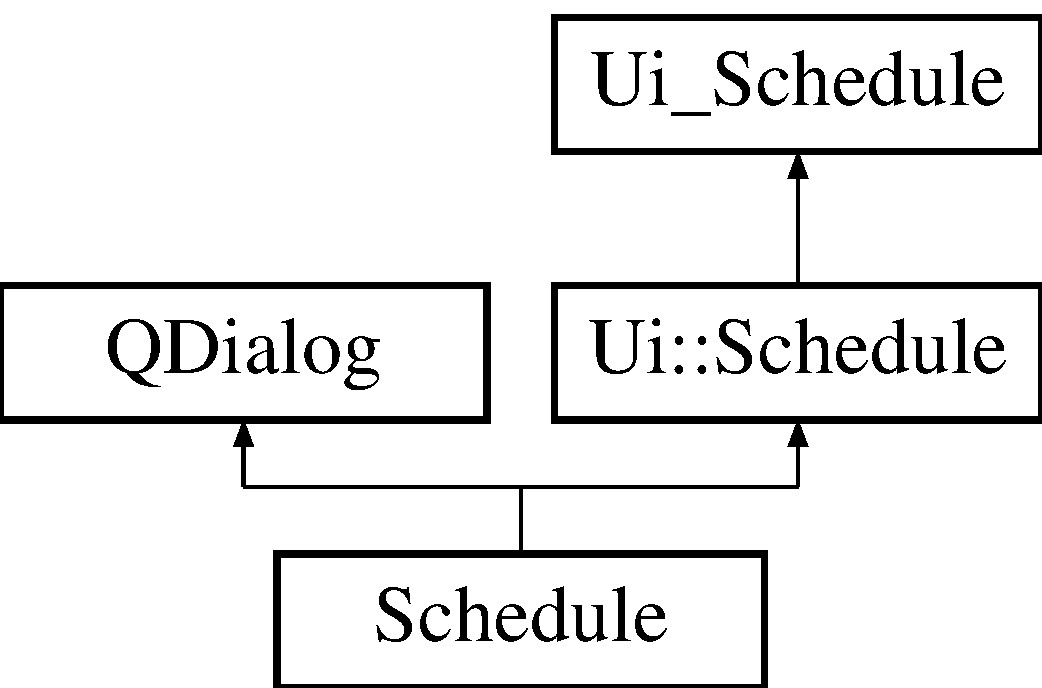
\includegraphics[height=3.000000cm]{class_schedule}
\end{center}
\end{figure}
\subsection*{Public Member Functions}
\begin{DoxyCompactItemize}
\item 
{\bf Schedule} ({\bf Controller} $\ast$controller, {\bf View} $\ast$parent=N\-U\-L\-L)
\item 
{\bf $\sim$\-Schedule} ()
\item 
void {\bf set\-List\-Of\-Courses} ()
\item 
void {\bf load\-From\-File\-Current\-State} ({\bf Deck} \&s, const char $\ast$filename)
\end{DoxyCompactItemize}
\subsection*{Private Attributes}
\begin{DoxyCompactItemize}
\item 
vector$<$ {\bf P\-Deck} $>$ {\bf vector\-Of\-Decks}
\item 
{\bf View} $\ast$ {\bf my\-View\-\_\-}
\item 
{\bf Controller} $\ast$ {\bf my\-Controller\-\_\-}
\item 
std\-::vector$<$ std\-::string $>$ {\bf files\-Txt}
\end{DoxyCompactItemize}
\subsection*{Additional Inherited Members}


\subsection{Constructor \& Destructor Documentation}
\index{Schedule@{Schedule}!Schedule@{Schedule}}
\index{Schedule@{Schedule}!Schedule@{Schedule}}
\subsubsection[{Schedule}]{\setlength{\rightskip}{0pt plus 5cm}Schedule\-::\-Schedule (
\begin{DoxyParamCaption}
\item[{{\bf Controller} $\ast$}]{controller, }
\item[{{\bf View} $\ast$}]{parent = {\ttfamily NULL}}
\end{DoxyParamCaption}
)}\label{class_schedule_ae9e7a682c32e4763182b2792bd37e89c}
\index{Schedule@{Schedule}!$\sim$\-Schedule@{$\sim$\-Schedule}}
\index{$\sim$\-Schedule@{$\sim$\-Schedule}!Schedule@{Schedule}}
\subsubsection[{$\sim$\-Schedule}]{\setlength{\rightskip}{0pt plus 5cm}Schedule\-::$\sim$\-Schedule (
\begin{DoxyParamCaption}
{}
\end{DoxyParamCaption}
)}\label{class_schedule_a4806b985197d35c00b9e707c0ed87998}


\subsection{Member Function Documentation}
\index{Schedule@{Schedule}!load\-From\-File\-Current\-State@{load\-From\-File\-Current\-State}}
\index{load\-From\-File\-Current\-State@{load\-From\-File\-Current\-State}!Schedule@{Schedule}}
\subsubsection[{load\-From\-File\-Current\-State}]{\setlength{\rightskip}{0pt plus 5cm}void Schedule\-::load\-From\-File\-Current\-State (
\begin{DoxyParamCaption}
\item[{{\bf Deck} \&}]{s, }
\item[{const char $\ast$}]{filename}
\end{DoxyParamCaption}
)}\label{class_schedule_aac4524cb4b65115e0b1a2a35ce98168a}
\index{Schedule@{Schedule}!set\-List\-Of\-Courses@{set\-List\-Of\-Courses}}
\index{set\-List\-Of\-Courses@{set\-List\-Of\-Courses}!Schedule@{Schedule}}
\subsubsection[{set\-List\-Of\-Courses}]{\setlength{\rightskip}{0pt plus 5cm}void Schedule\-::set\-List\-Of\-Courses (
\begin{DoxyParamCaption}
{}
\end{DoxyParamCaption}
)}\label{class_schedule_aadba5b3fbc8bfd56e8b9eb3aa58a6a86}


\subsection{Member Data Documentation}
\index{Schedule@{Schedule}!files\-Txt@{files\-Txt}}
\index{files\-Txt@{files\-Txt}!Schedule@{Schedule}}
\subsubsection[{files\-Txt}]{\setlength{\rightskip}{0pt plus 5cm}std\-::vector$<$std\-::string$>$ Schedule\-::files\-Txt\hspace{0.3cm}{\ttfamily [private]}}\label{class_schedule_a86220bb7cb3dced704dd06123a1054b6}
\index{Schedule@{Schedule}!my\-Controller\-\_\-@{my\-Controller\-\_\-}}
\index{my\-Controller\-\_\-@{my\-Controller\-\_\-}!Schedule@{Schedule}}
\subsubsection[{my\-Controller\-\_\-}]{\setlength{\rightskip}{0pt plus 5cm}{\bf Controller}$\ast$ Schedule\-::my\-Controller\-\_\-\hspace{0.3cm}{\ttfamily [private]}}\label{class_schedule_a1b193516f2917c8776186848127858f7}
\index{Schedule@{Schedule}!my\-View\-\_\-@{my\-View\-\_\-}}
\index{my\-View\-\_\-@{my\-View\-\_\-}!Schedule@{Schedule}}
\subsubsection[{my\-View\-\_\-}]{\setlength{\rightskip}{0pt plus 5cm}{\bf View}$\ast$ Schedule\-::my\-View\-\_\-\hspace{0.3cm}{\ttfamily [private]}}\label{class_schedule_a162220493359259792c99260fcf299ad}
\index{Schedule@{Schedule}!vector\-Of\-Decks@{vector\-Of\-Decks}}
\index{vector\-Of\-Decks@{vector\-Of\-Decks}!Schedule@{Schedule}}
\subsubsection[{vector\-Of\-Decks}]{\setlength{\rightskip}{0pt plus 5cm}vector$<${\bf P\-Deck}$>$ Schedule\-::vector\-Of\-Decks\hspace{0.3cm}{\ttfamily [private]}}\label{class_schedule_a025e8d4b7e6c047bcb3f0e62dc22fa64}


The documentation for this class was generated from the following files\-:\begin{DoxyCompactItemize}
\item 
Projekt\-Z\-P\-R/{\bf schedule.\-h}\item 
Projekt\-Z\-P\-R/{\bf schedule.\-cpp}\end{DoxyCompactItemize}

\section{Ui\-:\-:Schedule Class Reference}
\label{class_ui_1_1_schedule}\index{Ui\-::\-Schedule@{Ui\-::\-Schedule}}


{\ttfamily \#include $<$ui\-\_\-schedule.\-h$>$}

Inheritance diagram for Ui\-:\-:Schedule\-:\begin{figure}[H]
\begin{center}
\leavevmode
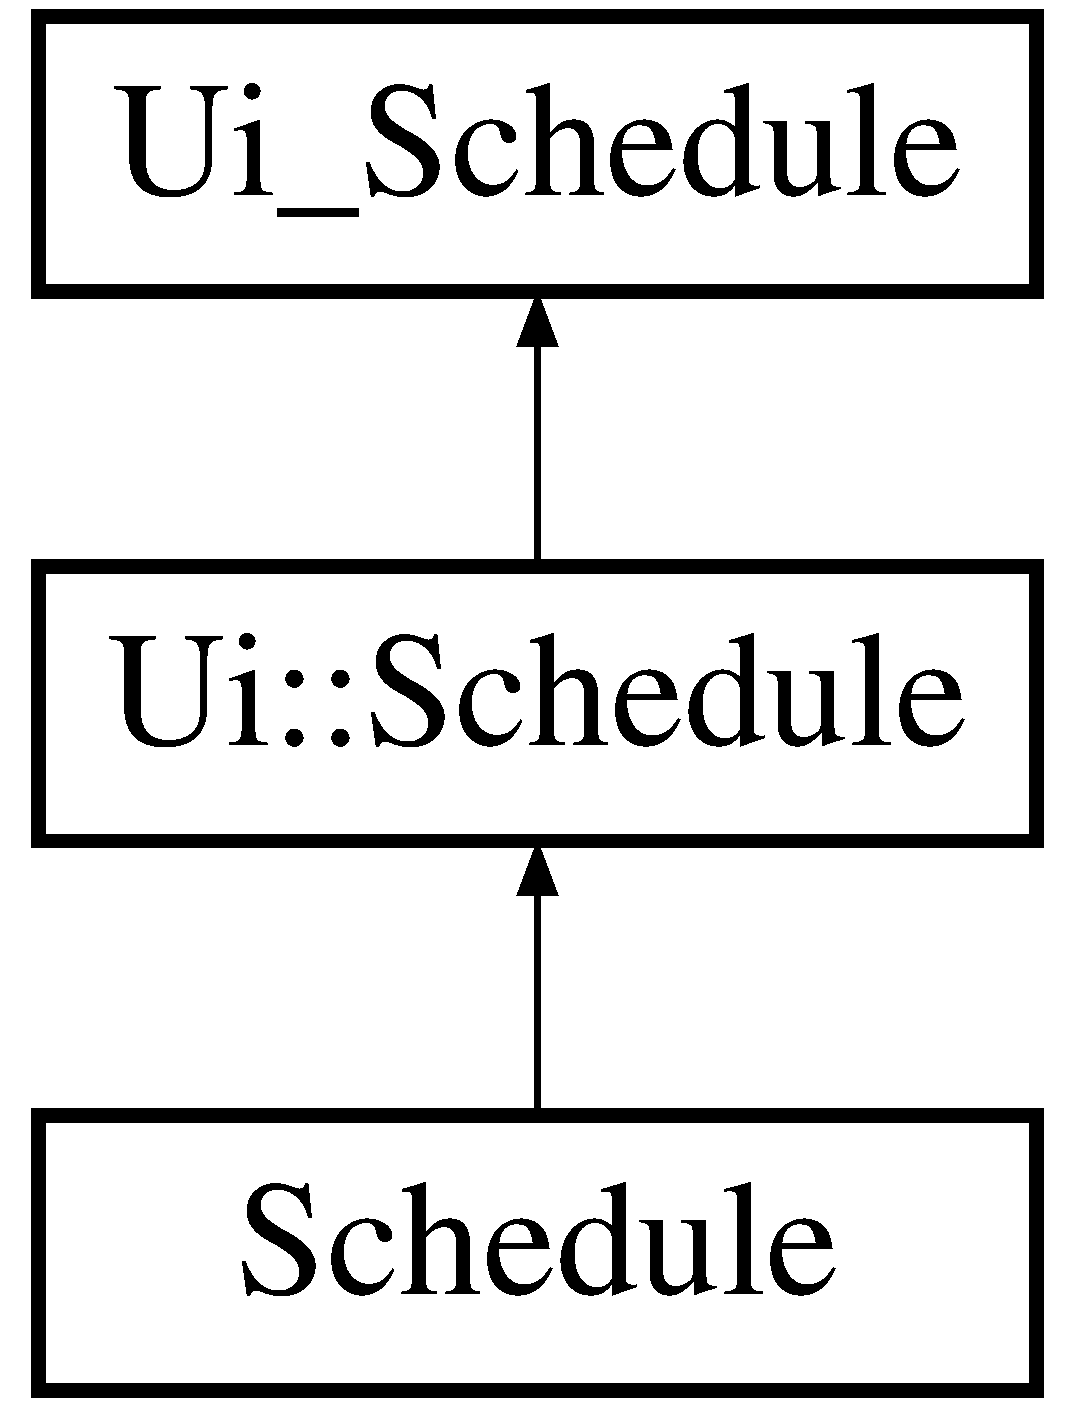
\includegraphics[height=3.000000cm]{class_ui_1_1_schedule}
\end{center}
\end{figure}
\subsection*{Additional Inherited Members}


The documentation for this class was generated from the following file\-:\begin{DoxyCompactItemize}
\item 
Projekt\-Z\-P\-R/\-Generated\-Files/{\bf ui\-\_\-schedule.\-h}\end{DoxyCompactItemize}

\section{Start Class Reference}
\label{class_start}\index{Start@{Start}}


{\ttfamily \#include $<$start.\-h$>$}

\subsection*{Public Member Functions}
\begin{DoxyCompactItemize}
\item 
{\bf Start} ()
\item 
{\bf $\sim$\-Start} ()
\item 
void {\bf set\-List\-Of\-Files} ()
\begin{DoxyCompactList}\small\item\em function to set lists of file in the course window \end{DoxyCompactList}\item 
std\-::vector$<$ std\-::string $>$ {\bf get\-List\-Of\-Files} ()
\begin{DoxyCompactList}\small\item\em function to get lists of file \end{DoxyCompactList}\item 
{\bf Deck} $\ast$ {\bf get\-Deck} ()
\begin{DoxyCompactList}\small\item\em function to get \doxyref{Deck}{p.}{class_deck} object \end{DoxyCompactList}\item 
{\bf P\-Deck} {\bf get\-Decknew} ()
\begin{DoxyCompactList}\small\item\em function to get P\-Deck object \end{DoxyCompactList}\item 
void {\bf choose\-Course} (std\-::string course, bool flag)
\begin{DoxyCompactList}\small\item\em function to perform action after choose button clicked \end{DoxyCompactList}\item 
void {\bf delete\-Course} (std\-::string course)
\begin{DoxyCompactList}\small\item\em function to perform action after delete button clicked \end{DoxyCompactList}\item 
void {\bf set\-Next\-Date\-For\-Each} (vector$<$ int $>$ answers\-Judged, std\-::string course\-Name)
\begin{DoxyCompactList}\small\item\em function to count next date for each question, implementation of S\-M2 algorithm \end{DoxyCompactList}\item 
void {\bf save\-To\-File\-Current\-State} (const {\bf Deck} \&s, const char $\ast$filename)
\begin{DoxyCompactList}\small\item\em serialization of current object state \end{DoxyCompactList}\item 
void {\bf load\-From\-File\-Current\-State} ({\bf Deck} \&s, const char $\ast$filename)
\begin{DoxyCompactList}\small\item\em load state of object from file \end{DoxyCompactList}\item 
void {\bf continue\-Clicked} (std\-::string name)
\begin{DoxyCompactList}\small\item\em function to perform action after continue button clicked \end{DoxyCompactList}\end{DoxyCompactItemize}
\subsection*{Public Attributes}
\begin{DoxyCompactItemize}
\item 
bool {\bf flag\-\_\-}
\begin{DoxyCompactList}\small\item\em field to protect from unwanted behaviour of aplication \end{DoxyCompactList}\end{DoxyCompactItemize}
\subsection*{Private Attributes}
\begin{DoxyCompactItemize}
\item 
std\-::vector$<$ std\-::string $>$ {\bf files\-Xml}
\begin{DoxyCompactList}\small\item\em vector of file which are about to be on courses list \end{DoxyCompactList}\item 
{\bf Deck} $\ast$ {\bf deck\-\_\-}
\item 
{\bf P\-Deck} {\bf decknew\-\_\-}
\end{DoxyCompactItemize}


\subsection{Detailed Description}
Class represents logic of \doxyref{Start}{p.}{class_start} Menu Dialog \begin{DoxyAuthor}{Author}
Piotr Maleci \& Michal Daniluk 
\end{DoxyAuthor}


\subsection{Constructor \& Destructor Documentation}
\index{Start@{Start}!Start@{Start}}
\index{Start@{Start}!Start@{Start}}
\subsubsection[{Start}]{\setlength{\rightskip}{0pt plus 5cm}Start\-::\-Start (
\begin{DoxyParamCaption}
{}
\end{DoxyParamCaption}
)}\label{class_start_a26acc6dcc887a9c9d140532a179cfe34}
\index{Start@{Start}!$\sim$\-Start@{$\sim$\-Start}}
\index{$\sim$\-Start@{$\sim$\-Start}!Start@{Start}}
\subsubsection[{$\sim$\-Start}]{\setlength{\rightskip}{0pt plus 5cm}Start\-::$\sim$\-Start (
\begin{DoxyParamCaption}
{}
\end{DoxyParamCaption}
)}\label{class_start_ad28971ef6d65a39a8a748d4992260f8c}


\subsection{Member Function Documentation}
\index{Start@{Start}!choose\-Course@{choose\-Course}}
\index{choose\-Course@{choose\-Course}!Start@{Start}}
\subsubsection[{choose\-Course}]{\setlength{\rightskip}{0pt plus 5cm}void Start\-::choose\-Course (
\begin{DoxyParamCaption}
\item[{std\-::string}]{course, }
\item[{bool}]{flag}
\end{DoxyParamCaption}
)}\label{class_start_ae34e97c88db29c6d8c9b647e3b22abc8}


function to perform action after choose button clicked 

\index{Start@{Start}!continue\-Clicked@{continue\-Clicked}}
\index{continue\-Clicked@{continue\-Clicked}!Start@{Start}}
\subsubsection[{continue\-Clicked}]{\setlength{\rightskip}{0pt plus 5cm}void Start\-::continue\-Clicked (
\begin{DoxyParamCaption}
\item[{std\-::string}]{name}
\end{DoxyParamCaption}
)}\label{class_start_ae434cdd7579b59bd2358497a9ca62ff2}


function to perform action after continue button clicked 

\index{Start@{Start}!delete\-Course@{delete\-Course}}
\index{delete\-Course@{delete\-Course}!Start@{Start}}
\subsubsection[{delete\-Course}]{\setlength{\rightskip}{0pt plus 5cm}void Start\-::delete\-Course (
\begin{DoxyParamCaption}
\item[{std\-::string}]{course}
\end{DoxyParamCaption}
)}\label{class_start_adf449dff62c491679bfab6c6365048bb}


function to perform action after delete button clicked 

\index{Start@{Start}!get\-Deck@{get\-Deck}}
\index{get\-Deck@{get\-Deck}!Start@{Start}}
\subsubsection[{get\-Deck}]{\setlength{\rightskip}{0pt plus 5cm}{\bf Deck}$\ast$ Start\-::get\-Deck (
\begin{DoxyParamCaption}
{}
\end{DoxyParamCaption}
)\hspace{0.3cm}{\ttfamily [inline]}}\label{class_start_aad74a0c9e127b2c6ff4b24cf545b130d}


function to get \doxyref{Deck}{p.}{class_deck} object 

\index{Start@{Start}!get\-Decknew@{get\-Decknew}}
\index{get\-Decknew@{get\-Decknew}!Start@{Start}}
\subsubsection[{get\-Decknew}]{\setlength{\rightskip}{0pt plus 5cm}{\bf P\-Deck} Start\-::get\-Decknew (
\begin{DoxyParamCaption}
{}
\end{DoxyParamCaption}
)\hspace{0.3cm}{\ttfamily [inline]}}\label{class_start_a0a91aa87cff930931881457639ba6e6c}


function to get P\-Deck object 

\index{Start@{Start}!get\-List\-Of\-Files@{get\-List\-Of\-Files}}
\index{get\-List\-Of\-Files@{get\-List\-Of\-Files}!Start@{Start}}
\subsubsection[{get\-List\-Of\-Files}]{\setlength{\rightskip}{0pt plus 5cm}std\-::vector$<$std\-::string$>$ Start\-::get\-List\-Of\-Files (
\begin{DoxyParamCaption}
{}
\end{DoxyParamCaption}
)\hspace{0.3cm}{\ttfamily [inline]}}\label{class_start_a1fc0c5c6250f3507c89baa502dc76a8a}


function to get lists of file 

\index{Start@{Start}!load\-From\-File\-Current\-State@{load\-From\-File\-Current\-State}}
\index{load\-From\-File\-Current\-State@{load\-From\-File\-Current\-State}!Start@{Start}}
\subsubsection[{load\-From\-File\-Current\-State}]{\setlength{\rightskip}{0pt plus 5cm}void Start\-::load\-From\-File\-Current\-State (
\begin{DoxyParamCaption}
\item[{{\bf Deck} \&}]{s, }
\item[{const char $\ast$}]{filename}
\end{DoxyParamCaption}
)}\label{class_start_ab6b6f1d081ca1b613629696e271a2def}


load state of object from file 

\index{Start@{Start}!save\-To\-File\-Current\-State@{save\-To\-File\-Current\-State}}
\index{save\-To\-File\-Current\-State@{save\-To\-File\-Current\-State}!Start@{Start}}
\subsubsection[{save\-To\-File\-Current\-State}]{\setlength{\rightskip}{0pt plus 5cm}void Start\-::save\-To\-File\-Current\-State (
\begin{DoxyParamCaption}
\item[{const {\bf Deck} \&}]{s, }
\item[{const char $\ast$}]{filename}
\end{DoxyParamCaption}
)}\label{class_start_abf3764f12336ace3d90d37724e020938}


serialization of current object state 

\index{Start@{Start}!set\-List\-Of\-Files@{set\-List\-Of\-Files}}
\index{set\-List\-Of\-Files@{set\-List\-Of\-Files}!Start@{Start}}
\subsubsection[{set\-List\-Of\-Files}]{\setlength{\rightskip}{0pt plus 5cm}void Start\-::set\-List\-Of\-Files (
\begin{DoxyParamCaption}
{}
\end{DoxyParamCaption}
)}\label{class_start_a8d285fb9b9ac9fe04947bb835f1c8e59}


function to set lists of file in the course window 

\index{Start@{Start}!set\-Next\-Date\-For\-Each@{set\-Next\-Date\-For\-Each}}
\index{set\-Next\-Date\-For\-Each@{set\-Next\-Date\-For\-Each}!Start@{Start}}
\subsubsection[{set\-Next\-Date\-For\-Each}]{\setlength{\rightskip}{0pt plus 5cm}void Start\-::set\-Next\-Date\-For\-Each (
\begin{DoxyParamCaption}
\item[{vector$<$ int $>$}]{answers\-Judged, }
\item[{std\-::string}]{course\-Name}
\end{DoxyParamCaption}
)}\label{class_start_ad7bead563cace80868b0c27755f5a226}


function to count next date for each question, implementation of S\-M2 algorithm 



\subsection{Member Data Documentation}
\index{Start@{Start}!deck\-\_\-@{deck\-\_\-}}
\index{deck\-\_\-@{deck\-\_\-}!Start@{Start}}
\subsubsection[{deck\-\_\-}]{\setlength{\rightskip}{0pt plus 5cm}{\bf Deck}$\ast$ Start\-::deck\-\_\-\hspace{0.3cm}{\ttfamily [private]}}\label{class_start_a456664134843f62e5e45107bdc849a0a}
\index{Start@{Start}!decknew\-\_\-@{decknew\-\_\-}}
\index{decknew\-\_\-@{decknew\-\_\-}!Start@{Start}}
\subsubsection[{decknew\-\_\-}]{\setlength{\rightskip}{0pt plus 5cm}{\bf P\-Deck} Start\-::decknew\-\_\-\hspace{0.3cm}{\ttfamily [private]}}\label{class_start_ab2fb4f580007a612df4cb2e20f513145}
\index{Start@{Start}!files\-Xml@{files\-Xml}}
\index{files\-Xml@{files\-Xml}!Start@{Start}}
\subsubsection[{files\-Xml}]{\setlength{\rightskip}{0pt plus 5cm}std\-::vector$<$std\-::string$>$ Start\-::files\-Xml\hspace{0.3cm}{\ttfamily [private]}}\label{class_start_a37eda4da9fb1f4b857ede3ac91608c26}


vector of file which are about to be on courses list 

\index{Start@{Start}!flag\-\_\-@{flag\-\_\-}}
\index{flag\-\_\-@{flag\-\_\-}!Start@{Start}}
\subsubsection[{flag\-\_\-}]{\setlength{\rightskip}{0pt plus 5cm}bool Start\-::flag\-\_\-}\label{class_start_afeb30c075329fbe519bf01a4869d2a64}


field to protect from unwanted behaviour of aplication 



The documentation for this class was generated from the following files\-:\begin{DoxyCompactItemize}
\item 
Projekt\-Z\-P\-R/{\bf start.\-h}\item 
Projekt\-Z\-P\-R/{\bf start.\-cpp}\end{DoxyCompactItemize}

\section{Ui\-:\-:Start\-Menu Class Reference}
\label{class_ui_1_1_start_menu}\index{Ui\-::\-Start\-Menu@{Ui\-::\-Start\-Menu}}


{\ttfamily \#include $<$ui\-\_\-startmenu.\-h$>$}

Inheritance diagram for Ui\-:\-:Start\-Menu\-:\begin{figure}[H]
\begin{center}
\leavevmode
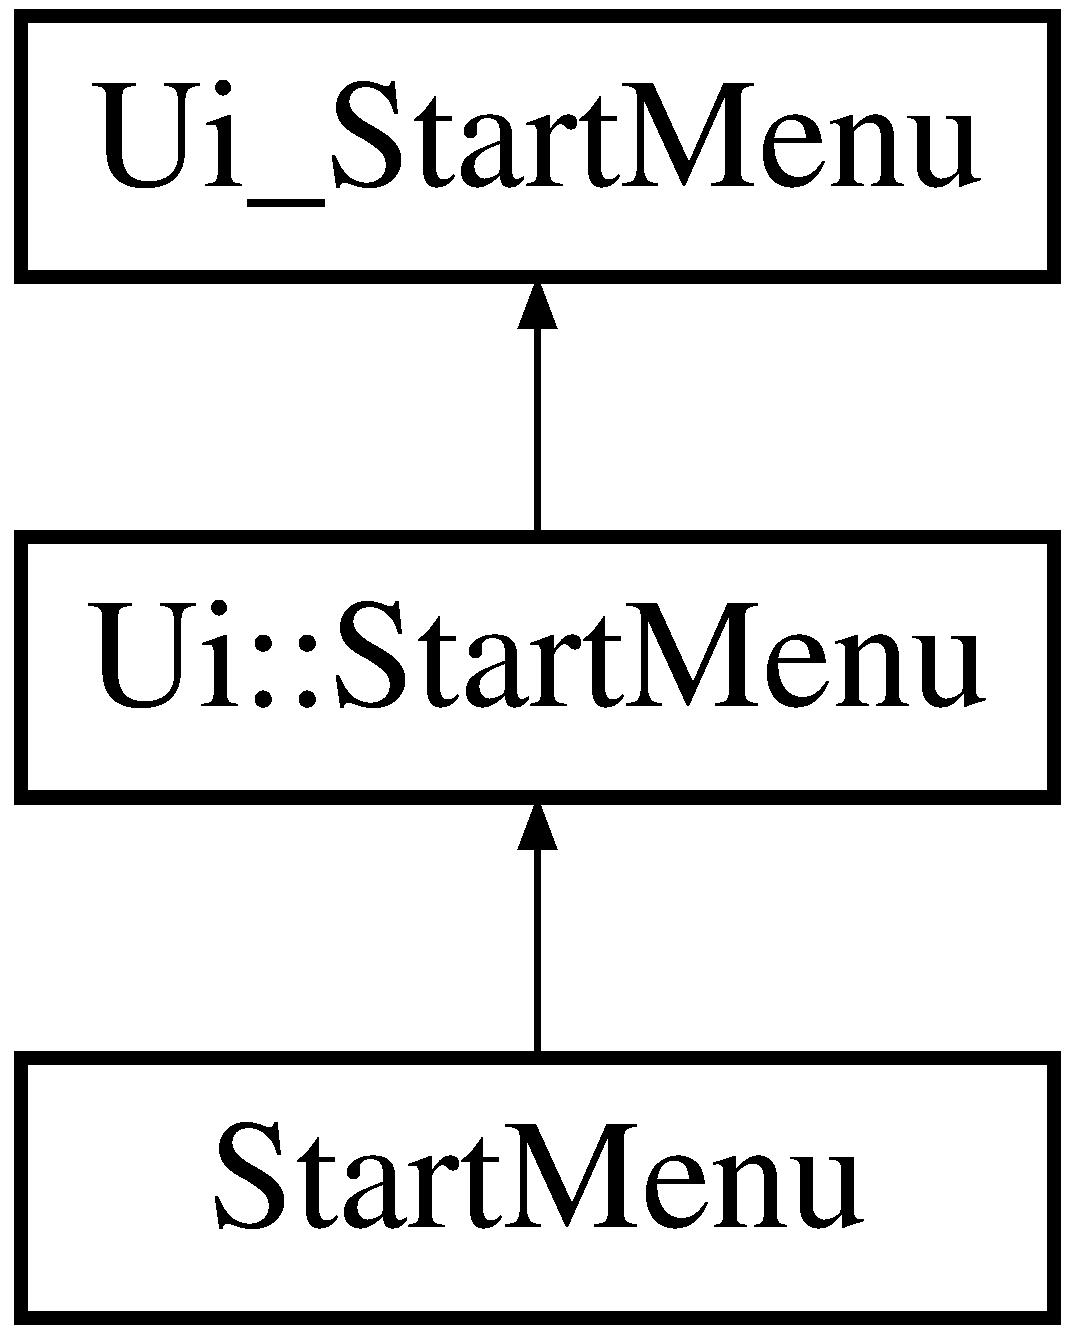
\includegraphics[height=3.000000cm]{class_ui_1_1_start_menu}
\end{center}
\end{figure}
\subsection*{Additional Inherited Members}


The documentation for this class was generated from the following file\-:\begin{DoxyCompactItemize}
\item 
Projekt\-Z\-P\-R/\-Generated\-Files/{\bf ui\-\_\-startmenu.\-h}\end{DoxyCompactItemize}

\section{Start\-Menu Class Reference}
\label{class_start_menu}\index{Start\-Menu@{Start\-Menu}}


{\ttfamily \#include $<$startmenu.\-h$>$}

Inheritance diagram for Start\-Menu\-:\begin{figure}[H]
\begin{center}
\leavevmode
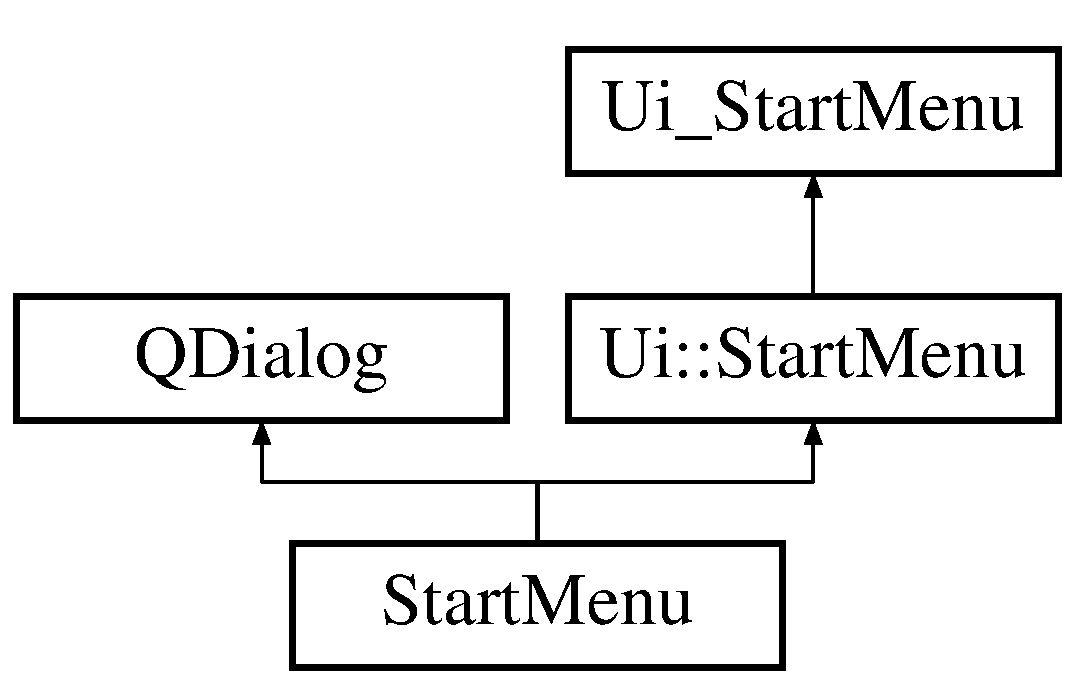
\includegraphics[height=3.000000cm]{class_start_menu}
\end{center}
\end{figure}
\subsection*{Public Slots}
\begin{DoxyCompactItemize}
\item 
void {\bf set\-List\-Of\-Courses} (std\-::vector$<$ std\-::string $>$ list\-Of\-Files)
\item 
void {\bf close\-Window} ()
\end{DoxyCompactItemize}
\subsection*{Signals}
\begin{DoxyCompactItemize}
\item 
void {\bf show\-List\-Of\-Files} ()
\item 
void {\bf choose} (std\-::string, bool)
\item 
void {\bf choose\-Continue} (std\-::string)
\item 
void {\bf close\-Start} ()
\item 
void {\bf delete\-Course} (std\-::string)
\end{DoxyCompactItemize}
\subsection*{Public Member Functions}
\begin{DoxyCompactItemize}
\item 
{\bf Start\-Menu} ({\bf Controller} $\ast$controller, {\bf View} $\ast$parent=N\-U\-L\-L)
\item 
{\bf $\sim$\-Start\-Menu} ()
\end{DoxyCompactItemize}
\subsection*{Protected Member Functions}
\begin{DoxyCompactItemize}
\item 
void {\bf close\-Event} (Q\-Close\-Event $\ast$event)
\end{DoxyCompactItemize}
\subsection*{Private Slots}
\begin{DoxyCompactItemize}
\item 
void {\bf on\-\_\-choose\-\_\-clicked} ()
\item 
void {\bf on\-\_\-continue\-Button\-\_\-clicked} ()
\item 
void {\bf on\-\_\-delete\-Button\-\_\-clicked} ()
\end{DoxyCompactItemize}
\subsection*{Private Attributes}
\begin{DoxyCompactItemize}
\item 
{\bf View} $\ast$ {\bf my\-View\-\_\-}
\item 
{\bf Controller} $\ast$ {\bf my\-Controller\-\_\-}
\end{DoxyCompactItemize}
\subsection*{Additional Inherited Members}


\subsection{Detailed Description}
Class represents start menu dialog. \begin{DoxyAuthor}{Author}
Piotr Maleci \& Michal Daniluk 
\end{DoxyAuthor}


\subsection{Constructor \& Destructor Documentation}
\index{Start\-Menu@{Start\-Menu}!Start\-Menu@{Start\-Menu}}
\index{Start\-Menu@{Start\-Menu}!StartMenu@{Start\-Menu}}
\subsubsection[{Start\-Menu}]{\setlength{\rightskip}{0pt plus 5cm}Start\-Menu\-::\-Start\-Menu (
\begin{DoxyParamCaption}
\item[{{\bf Controller} $\ast$}]{controller, }
\item[{{\bf View} $\ast$}]{parent = {\ttfamily NULL}}
\end{DoxyParamCaption}
)}\label{class_start_menu_a1e8aab02fee6433f78b05a2705a226cc}
\index{Start\-Menu@{Start\-Menu}!$\sim$\-Start\-Menu@{$\sim$\-Start\-Menu}}
\index{$\sim$\-Start\-Menu@{$\sim$\-Start\-Menu}!StartMenu@{Start\-Menu}}
\subsubsection[{$\sim$\-Start\-Menu}]{\setlength{\rightskip}{0pt plus 5cm}Start\-Menu\-::$\sim$\-Start\-Menu (
\begin{DoxyParamCaption}
{}
\end{DoxyParamCaption}
)}\label{class_start_menu_a0586b30fd5cedbb22ad3a22c98913481}


\subsection{Member Function Documentation}
\index{Start\-Menu@{Start\-Menu}!choose@{choose}}
\index{choose@{choose}!StartMenu@{Start\-Menu}}
\subsubsection[{choose}]{\setlength{\rightskip}{0pt plus 5cm}void Start\-Menu\-::choose (
\begin{DoxyParamCaption}
\item[{std\-::string}]{\-\_\-t1, }
\item[{bool}]{\-\_\-t2}
\end{DoxyParamCaption}
)\hspace{0.3cm}{\ttfamily [signal]}}\label{class_start_menu_a9636a82f457c9f302091e6bcd2e887eb}
\index{Start\-Menu@{Start\-Menu}!choose\-Continue@{choose\-Continue}}
\index{choose\-Continue@{choose\-Continue}!StartMenu@{Start\-Menu}}
\subsubsection[{choose\-Continue}]{\setlength{\rightskip}{0pt plus 5cm}void Start\-Menu\-::choose\-Continue (
\begin{DoxyParamCaption}
\item[{std\-::string}]{\-\_\-t1}
\end{DoxyParamCaption}
)\hspace{0.3cm}{\ttfamily [signal]}}\label{class_start_menu_a0c06234ebc3c68d6259167571b54454e}
\index{Start\-Menu@{Start\-Menu}!close\-Event@{close\-Event}}
\index{close\-Event@{close\-Event}!StartMenu@{Start\-Menu}}
\subsubsection[{close\-Event}]{\setlength{\rightskip}{0pt plus 5cm}void Start\-Menu\-::close\-Event (
\begin{DoxyParamCaption}
\item[{Q\-Close\-Event $\ast$}]{event}
\end{DoxyParamCaption}
)\hspace{0.3cm}{\ttfamily [protected]}}\label{class_start_menu_a4e1479681b0bf8b2493a8589c1a61adc}
\index{Start\-Menu@{Start\-Menu}!close\-Start@{close\-Start}}
\index{close\-Start@{close\-Start}!StartMenu@{Start\-Menu}}
\subsubsection[{close\-Start}]{\setlength{\rightskip}{0pt plus 5cm}void Start\-Menu\-::close\-Start (
\begin{DoxyParamCaption}
{}
\end{DoxyParamCaption}
)\hspace{0.3cm}{\ttfamily [signal]}}\label{class_start_menu_a59682c8c3d87da802947a1aefd5771a6}
\index{Start\-Menu@{Start\-Menu}!close\-Window@{close\-Window}}
\index{close\-Window@{close\-Window}!StartMenu@{Start\-Menu}}
\subsubsection[{close\-Window}]{\setlength{\rightskip}{0pt plus 5cm}void Start\-Menu\-::close\-Window (
\begin{DoxyParamCaption}
{}
\end{DoxyParamCaption}
)\hspace{0.3cm}{\ttfamily [slot]}}\label{class_start_menu_a5013e6965f128b801cfee2ebb0f9f373}
\index{Start\-Menu@{Start\-Menu}!delete\-Course@{delete\-Course}}
\index{delete\-Course@{delete\-Course}!StartMenu@{Start\-Menu}}
\subsubsection[{delete\-Course}]{\setlength{\rightskip}{0pt plus 5cm}void Start\-Menu\-::delete\-Course (
\begin{DoxyParamCaption}
\item[{std\-::string}]{\-\_\-t1}
\end{DoxyParamCaption}
)\hspace{0.3cm}{\ttfamily [signal]}}\label{class_start_menu_a2afa98577a9fa5b7ba8cb30235e37e09}
\index{Start\-Menu@{Start\-Menu}!on\-\_\-choose\-\_\-clicked@{on\-\_\-choose\-\_\-clicked}}
\index{on\-\_\-choose\-\_\-clicked@{on\-\_\-choose\-\_\-clicked}!StartMenu@{Start\-Menu}}
\subsubsection[{on\-\_\-choose\-\_\-clicked}]{\setlength{\rightskip}{0pt plus 5cm}void Start\-Menu\-::on\-\_\-choose\-\_\-clicked (
\begin{DoxyParamCaption}
{}
\end{DoxyParamCaption}
)\hspace{0.3cm}{\ttfamily [private]}, {\ttfamily [slot]}}\label{class_start_menu_ad575601c28f91b604c21bfc6ebebc0dd}
\index{Start\-Menu@{Start\-Menu}!on\-\_\-continue\-Button\-\_\-clicked@{on\-\_\-continue\-Button\-\_\-clicked}}
\index{on\-\_\-continue\-Button\-\_\-clicked@{on\-\_\-continue\-Button\-\_\-clicked}!StartMenu@{Start\-Menu}}
\subsubsection[{on\-\_\-continue\-Button\-\_\-clicked}]{\setlength{\rightskip}{0pt plus 5cm}void Start\-Menu\-::on\-\_\-continue\-Button\-\_\-clicked (
\begin{DoxyParamCaption}
{}
\end{DoxyParamCaption}
)\hspace{0.3cm}{\ttfamily [private]}, {\ttfamily [slot]}}\label{class_start_menu_a5127d4820b5c0606e0908d0cedf359b1}
\index{Start\-Menu@{Start\-Menu}!on\-\_\-delete\-Button\-\_\-clicked@{on\-\_\-delete\-Button\-\_\-clicked}}
\index{on\-\_\-delete\-Button\-\_\-clicked@{on\-\_\-delete\-Button\-\_\-clicked}!StartMenu@{Start\-Menu}}
\subsubsection[{on\-\_\-delete\-Button\-\_\-clicked}]{\setlength{\rightskip}{0pt plus 5cm}void Start\-Menu\-::on\-\_\-delete\-Button\-\_\-clicked (
\begin{DoxyParamCaption}
{}
\end{DoxyParamCaption}
)\hspace{0.3cm}{\ttfamily [private]}, {\ttfamily [slot]}}\label{class_start_menu_a49019953b58cab4f2cca079041cab4c4}
\index{Start\-Menu@{Start\-Menu}!set\-List\-Of\-Courses@{set\-List\-Of\-Courses}}
\index{set\-List\-Of\-Courses@{set\-List\-Of\-Courses}!StartMenu@{Start\-Menu}}
\subsubsection[{set\-List\-Of\-Courses}]{\setlength{\rightskip}{0pt plus 5cm}void Start\-Menu\-::set\-List\-Of\-Courses (
\begin{DoxyParamCaption}
\item[{std\-::vector$<$ std\-::string $>$}]{list\-Of\-Files}
\end{DoxyParamCaption}
)\hspace{0.3cm}{\ttfamily [slot]}}\label{class_start_menu_a8ceadba505c2d0411a8194de981ab98a}
\index{Start\-Menu@{Start\-Menu}!show\-List\-Of\-Files@{show\-List\-Of\-Files}}
\index{show\-List\-Of\-Files@{show\-List\-Of\-Files}!StartMenu@{Start\-Menu}}
\subsubsection[{show\-List\-Of\-Files}]{\setlength{\rightskip}{0pt plus 5cm}void Start\-Menu\-::show\-List\-Of\-Files (
\begin{DoxyParamCaption}
{}
\end{DoxyParamCaption}
)\hspace{0.3cm}{\ttfamily [signal]}}\label{class_start_menu_adaa4d7657672a7dcbce5d5835be69caf}


\subsection{Member Data Documentation}
\index{Start\-Menu@{Start\-Menu}!my\-Controller\-\_\-@{my\-Controller\-\_\-}}
\index{my\-Controller\-\_\-@{my\-Controller\-\_\-}!StartMenu@{Start\-Menu}}
\subsubsection[{my\-Controller\-\_\-}]{\setlength{\rightskip}{0pt plus 5cm}{\bf Controller}$\ast$ Start\-Menu\-::my\-Controller\-\_\-\hspace{0.3cm}{\ttfamily [private]}}\label{class_start_menu_a175f033340fdbeae0d9264001c9aed27}
\index{Start\-Menu@{Start\-Menu}!my\-View\-\_\-@{my\-View\-\_\-}}
\index{my\-View\-\_\-@{my\-View\-\_\-}!StartMenu@{Start\-Menu}}
\subsubsection[{my\-View\-\_\-}]{\setlength{\rightskip}{0pt plus 5cm}{\bf View}$\ast$ Start\-Menu\-::my\-View\-\_\-\hspace{0.3cm}{\ttfamily [private]}}\label{class_start_menu_a686aafb8e0a2ae7ed6f9ba40e6369734}


The documentation for this class was generated from the following files\-:\begin{DoxyCompactItemize}
\item 
Projekt\-Z\-P\-R/{\bf startmenu.\-h}\item 
Projekt\-Z\-P\-R/\-Generated\-Files/\-Debug/{\bf moc\-\_\-startmenu.\-cpp}\item 
Projekt\-Z\-P\-R/\-Generated\-Files/\-Release/{\bf moc\-\_\-startmenu.\-cpp}\item 
Projekt\-Z\-P\-R/\-Generated\-Files/\-Testy\-Z\-P\-R/{\bf moc\-\_\-startmenu.\-cpp}\item 
Projekt\-Z\-P\-R/\-Generated\-Files/\-Testy\-Z\-P\-R2/{\bf moc\-\_\-startmenu.\-cpp}\item 
Projekt\-Z\-P\-R/{\bf startmenu.\-cpp}\end{DoxyCompactItemize}

\section{Ui\-:\-:Statistic Class Reference}
\label{class_ui_1_1_statistic}\index{Ui\-::\-Statistic@{Ui\-::\-Statistic}}


{\ttfamily \#include $<$ui\-\_\-statistic.\-h$>$}

Inheritance diagram for Ui\-:\-:Statistic\-:\begin{figure}[H]
\begin{center}
\leavevmode
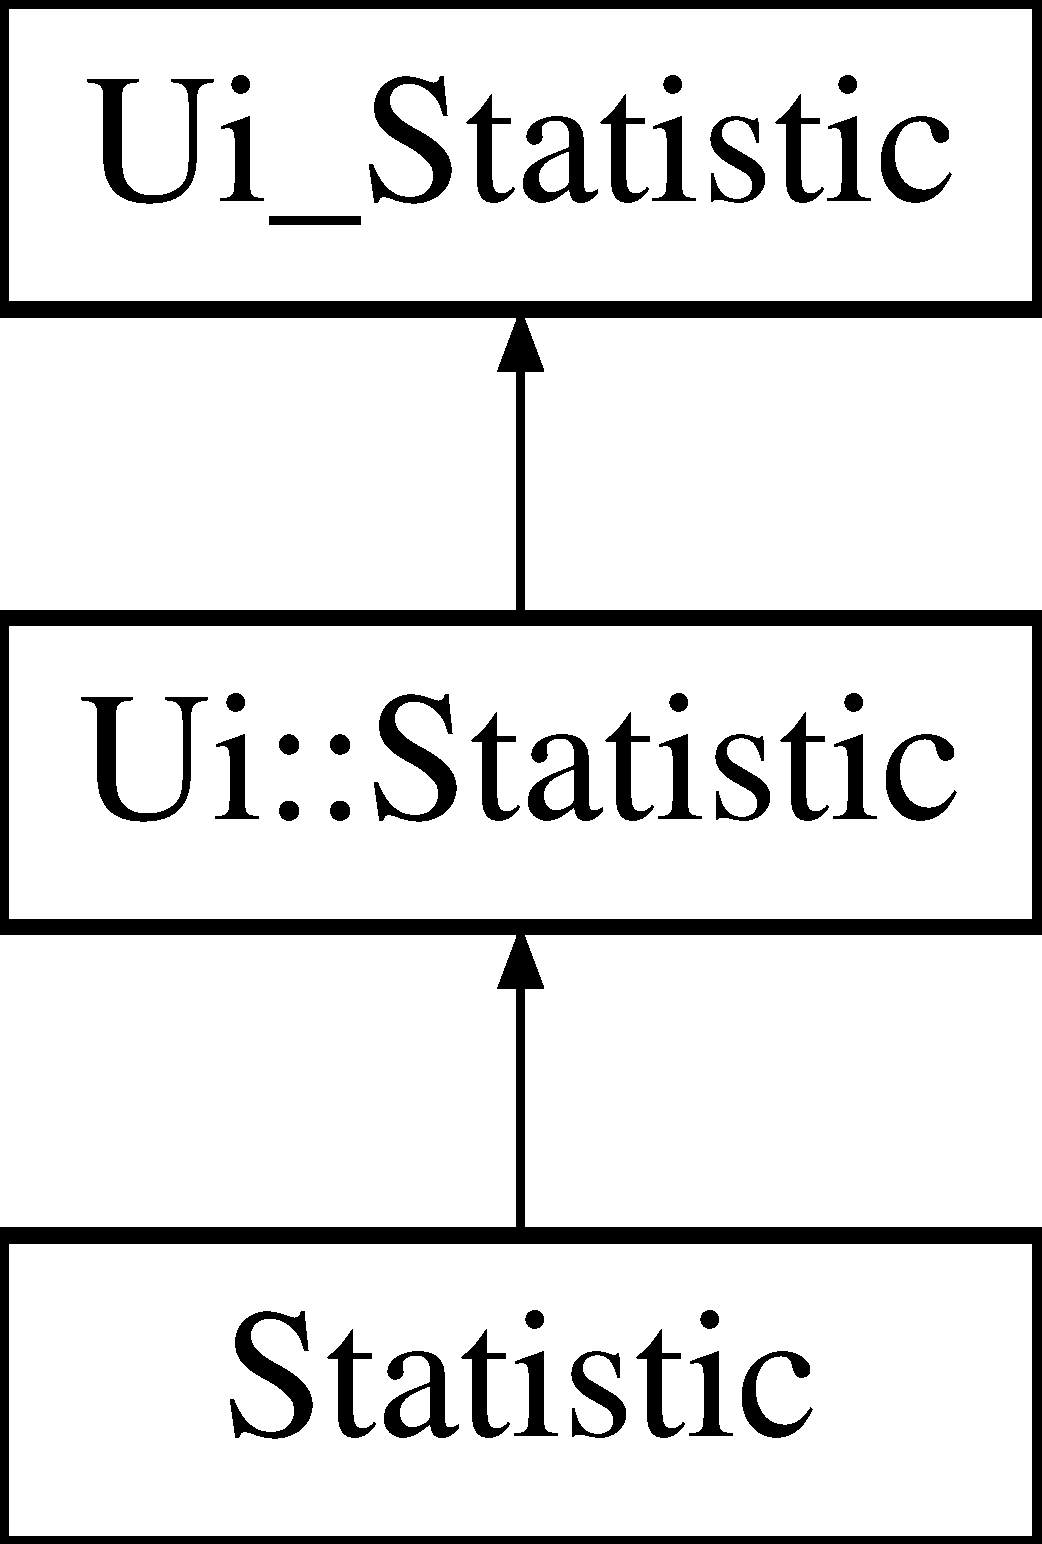
\includegraphics[height=3.000000cm]{class_ui_1_1_statistic}
\end{center}
\end{figure}
\subsection*{Additional Inherited Members}


The documentation for this class was generated from the following file\-:\begin{DoxyCompactItemize}
\item 
Projekt\-Z\-P\-R/\-Generated\-Files/{\bf ui\-\_\-statistic.\-h}\end{DoxyCompactItemize}

\section{Statistic Class Reference}
\label{class_statistic}\index{Statistic@{Statistic}}


{\ttfamily \#include $<$statistic.\-h$>$}

Inheritance diagram for Statistic\-:\begin{figure}[H]
\begin{center}
\leavevmode
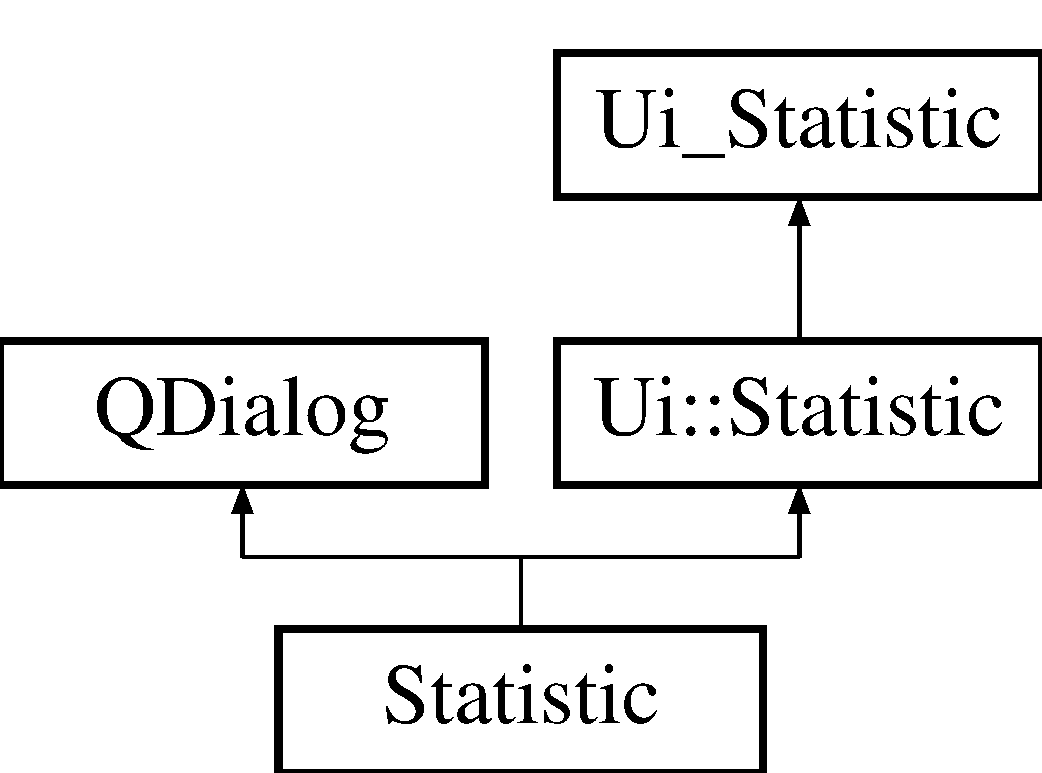
\includegraphics[height=3.000000cm]{class_statistic}
\end{center}
\end{figure}
\subsection*{Public Slots}
\begin{DoxyCompactItemize}
\item 
void {\bf show\-Statistic} (vector$<$ int $>$)
\end{DoxyCompactItemize}
\subsection*{Public Member Functions}
\begin{DoxyCompactItemize}
\item 
{\bf Statistic} ({\bf Controller} $\ast$controller, {\bf View} $\ast$parent=N\-U\-L\-L)
\item 
{\bf $\sim$\-Statistic} ()
\end{DoxyCompactItemize}
\subsection*{Private Attributes}
\begin{DoxyCompactItemize}
\item 
{\bf View} $\ast$ {\bf my\-View\-\_\-}
\item 
{\bf Controller} $\ast$ {\bf my\-Controller\-\_\-}
\end{DoxyCompactItemize}
\subsection*{Additional Inherited Members}


\subsection{Detailed Description}
Class represents \doxyref{Statistic}{p.}{class_statistic} \begin{DoxyAuthor}{Author}
Piotr Maleci \& Michal Daniluk 
\end{DoxyAuthor}


\subsection{Constructor \& Destructor Documentation}
\index{Statistic@{Statistic}!Statistic@{Statistic}}
\index{Statistic@{Statistic}!Statistic@{Statistic}}
\subsubsection[{Statistic}]{\setlength{\rightskip}{0pt plus 5cm}Statistic\-::\-Statistic (
\begin{DoxyParamCaption}
\item[{{\bf Controller} $\ast$}]{controller, }
\item[{{\bf View} $\ast$}]{parent = {\ttfamily NULL}}
\end{DoxyParamCaption}
)}\label{class_statistic_aceaa9c8508d7d8bfab779106ae97ce79}
\index{Statistic@{Statistic}!$\sim$\-Statistic@{$\sim$\-Statistic}}
\index{$\sim$\-Statistic@{$\sim$\-Statistic}!Statistic@{Statistic}}
\subsubsection[{$\sim$\-Statistic}]{\setlength{\rightskip}{0pt plus 5cm}Statistic\-::$\sim$\-Statistic (
\begin{DoxyParamCaption}
{}
\end{DoxyParamCaption}
)}\label{class_statistic_a273cc8bd352a4fa0c18006971c008424}


\subsection{Member Function Documentation}
\index{Statistic@{Statistic}!show\-Statistic@{show\-Statistic}}
\index{show\-Statistic@{show\-Statistic}!Statistic@{Statistic}}
\subsubsection[{show\-Statistic}]{\setlength{\rightskip}{0pt plus 5cm}void Statistic\-::show\-Statistic (
\begin{DoxyParamCaption}
\item[{vector$<$ int $>$}]{marks}
\end{DoxyParamCaption}
)\hspace{0.3cm}{\ttfamily [slot]}}\label{class_statistic_a5c3750d0241246f162e66260bf385ea6}


\subsection{Member Data Documentation}
\index{Statistic@{Statistic}!my\-Controller\-\_\-@{my\-Controller\-\_\-}}
\index{my\-Controller\-\_\-@{my\-Controller\-\_\-}!Statistic@{Statistic}}
\subsubsection[{my\-Controller\-\_\-}]{\setlength{\rightskip}{0pt plus 5cm}{\bf Controller}$\ast$ Statistic\-::my\-Controller\-\_\-\hspace{0.3cm}{\ttfamily [private]}}\label{class_statistic_a67be9f161046b43b2680072da8ae8a3d}
\index{Statistic@{Statistic}!my\-View\-\_\-@{my\-View\-\_\-}}
\index{my\-View\-\_\-@{my\-View\-\_\-}!Statistic@{Statistic}}
\subsubsection[{my\-View\-\_\-}]{\setlength{\rightskip}{0pt plus 5cm}{\bf View}$\ast$ Statistic\-::my\-View\-\_\-\hspace{0.3cm}{\ttfamily [private]}}\label{class_statistic_abd6276e25289835ab5a06ea50e6c913b}


The documentation for this class was generated from the following files\-:\begin{DoxyCompactItemize}
\item 
Projekt\-Z\-P\-R/{\bf statistic.\-h}\item 
Projekt\-Z\-P\-R/{\bf statistic.\-cpp}\end{DoxyCompactItemize}

\section{Ui\-\_\-\-Create\-Test Class Reference}
\label{class_ui___create_test}\index{Ui\-\_\-\-Create\-Test@{Ui\-\_\-\-Create\-Test}}


{\ttfamily \#include $<$ui\-\_\-createtest.\-h$>$}

Inheritance diagram for Ui\-\_\-\-Create\-Test\-:\begin{figure}[H]
\begin{center}
\leavevmode
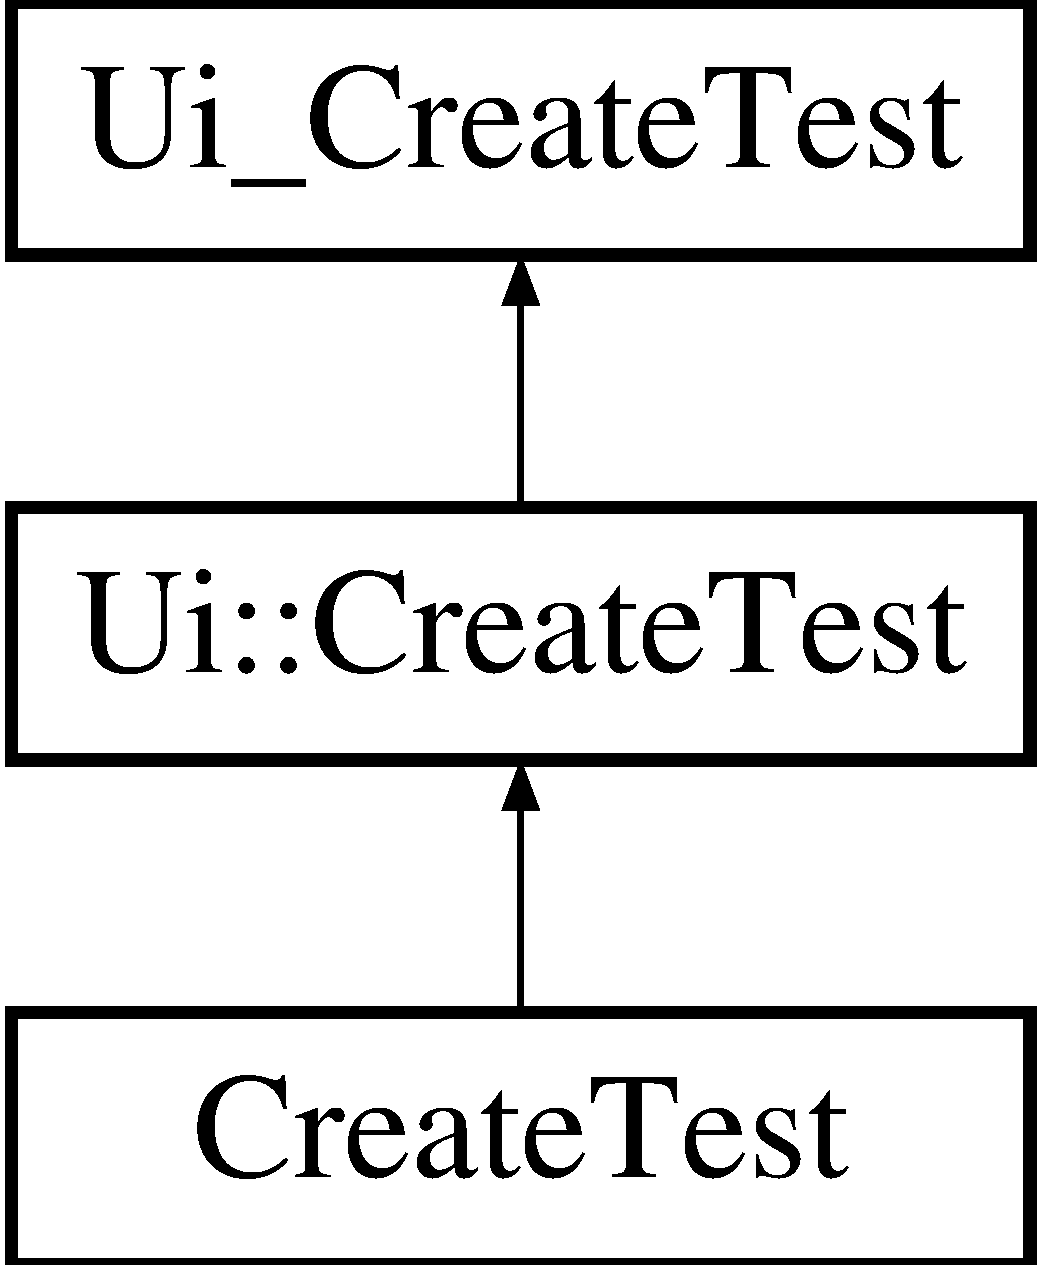
\includegraphics[height=3.000000cm]{class_ui___create_test}
\end{center}
\end{figure}
\subsection*{Public Member Functions}
\begin{DoxyCompactItemize}
\item 
void {\bf setup\-Ui} (Q\-Widget $\ast${\bf Create\-Test})
\item 
void {\bf retranslate\-Ui} (Q\-Widget $\ast${\bf Create\-Test})
\end{DoxyCompactItemize}
\subsection*{Public Attributes}
\begin{DoxyCompactItemize}
\item 
Q\-Label $\ast$ {\bf question\-Number}
\item 
Q\-Text\-Edit $\ast$ {\bf question\-Edit}
\item 
Q\-Push\-Button $\ast$ {\bf save}
\item 
Q\-Label $\ast$ {\bf label}
\item 
Q\-Tab\-Widget $\ast$ {\bf tabs}
\item 
Q\-Widget $\ast$ {\bf open}
\item 
Q\-V\-Box\-Layout $\ast$ {\bf vertical\-Layout}
\item 
Q\-Text\-Edit $\ast$ {\bf answer\-Open\-Edit}
\item 
Q\-Widget $\ast$ {\bf close}
\item 
Q\-Label $\ast$ {\bf label\-\_\-3}
\item 
Q\-Widget $\ast$ {\bf layout\-Widget}
\item 
Q\-Grid\-Layout $\ast$ {\bf grid\-Layout}
\item 
Q\-Label $\ast$ {\bf label\-\_\-4}
\item 
Q\-Label $\ast$ {\bf label\-\_\-5}
\item 
Q\-Label $\ast$ {\bf label\-\_\-6}
\item 
Q\-Label $\ast$ {\bf label\-\_\-7}
\item 
Q\-Widget $\ast$ {\bf layout\-Widget\-\_\-2}
\item 
Q\-Grid\-Layout $\ast$ {\bf grid\-Layout\-\_\-3}
\item 
Q\-Combo\-Box $\ast$ {\bf a\-Value}
\item 
Q\-Combo\-Box $\ast$ {\bf b\-Value}
\item 
Q\-Combo\-Box $\ast$ {\bf c\-Value}
\item 
Q\-Combo\-Box $\ast$ {\bf d\-Value}
\item 
Q\-Widget $\ast$ {\bf layout\-Widget\-\_\-3}
\item 
Q\-Grid\-Layout $\ast$ {\bf grid\-Layout\-\_\-2}
\item 
Q\-Text\-Edit $\ast$ {\bf answer\-Close\-A\-Edit}
\item 
Q\-Text\-Edit $\ast$ {\bf answer\-Close\-B\-Edit}
\item 
Q\-Text\-Edit $\ast$ {\bf answer\-Close\-C\-Edit}
\item 
Q\-Text\-Edit $\ast$ {\bf answer\-Close\-D\-Edit}
\item 
Q\-Label $\ast$ {\bf label\-\_\-2}
\item 
Q\-Push\-Button $\ast$ {\bf help}
\item 
Q\-Widget $\ast$ {\bf layout\-Widget\-\_\-4}
\item 
Q\-H\-Box\-Layout $\ast$ {\bf horizontal\-Layout}
\item 
Q\-Push\-Button $\ast$ {\bf back}
\item 
Q\-Push\-Button $\ast$ {\bf next}
\end{DoxyCompactItemize}


\subsection{Member Function Documentation}
\index{Ui\-\_\-\-Create\-Test@{Ui\-\_\-\-Create\-Test}!retranslate\-Ui@{retranslate\-Ui}}
\index{retranslate\-Ui@{retranslate\-Ui}!Ui_CreateTest@{Ui\-\_\-\-Create\-Test}}
\subsubsection[{retranslate\-Ui}]{\setlength{\rightskip}{0pt plus 5cm}void Ui\-\_\-\-Create\-Test\-::retranslate\-Ui (
\begin{DoxyParamCaption}
\item[{Q\-Widget $\ast$}]{Create\-Test}
\end{DoxyParamCaption}
)\hspace{0.3cm}{\ttfamily [inline]}}\label{class_ui___create_test_a6253c39fa579650a1dacf2eb586ab074}
\index{Ui\-\_\-\-Create\-Test@{Ui\-\_\-\-Create\-Test}!setup\-Ui@{setup\-Ui}}
\index{setup\-Ui@{setup\-Ui}!Ui_CreateTest@{Ui\-\_\-\-Create\-Test}}
\subsubsection[{setup\-Ui}]{\setlength{\rightskip}{0pt plus 5cm}void Ui\-\_\-\-Create\-Test\-::setup\-Ui (
\begin{DoxyParamCaption}
\item[{Q\-Widget $\ast$}]{Create\-Test}
\end{DoxyParamCaption}
)\hspace{0.3cm}{\ttfamily [inline]}}\label{class_ui___create_test_abb2ff0754b7bd0bc91a76fc196f08fd3}


\subsection{Member Data Documentation}
\index{Ui\-\_\-\-Create\-Test@{Ui\-\_\-\-Create\-Test}!answer\-Close\-A\-Edit@{answer\-Close\-A\-Edit}}
\index{answer\-Close\-A\-Edit@{answer\-Close\-A\-Edit}!Ui_CreateTest@{Ui\-\_\-\-Create\-Test}}
\subsubsection[{answer\-Close\-A\-Edit}]{\setlength{\rightskip}{0pt plus 5cm}Q\-Text\-Edit$\ast$ Ui\-\_\-\-Create\-Test\-::answer\-Close\-A\-Edit}\label{class_ui___create_test_a1c0919f04f3b529cfa2b5369789e462b}
\index{Ui\-\_\-\-Create\-Test@{Ui\-\_\-\-Create\-Test}!answer\-Close\-B\-Edit@{answer\-Close\-B\-Edit}}
\index{answer\-Close\-B\-Edit@{answer\-Close\-B\-Edit}!Ui_CreateTest@{Ui\-\_\-\-Create\-Test}}
\subsubsection[{answer\-Close\-B\-Edit}]{\setlength{\rightskip}{0pt plus 5cm}Q\-Text\-Edit$\ast$ Ui\-\_\-\-Create\-Test\-::answer\-Close\-B\-Edit}\label{class_ui___create_test_aa3634100fb651c860f6f4b5dc69441df}
\index{Ui\-\_\-\-Create\-Test@{Ui\-\_\-\-Create\-Test}!answer\-Close\-C\-Edit@{answer\-Close\-C\-Edit}}
\index{answer\-Close\-C\-Edit@{answer\-Close\-C\-Edit}!Ui_CreateTest@{Ui\-\_\-\-Create\-Test}}
\subsubsection[{answer\-Close\-C\-Edit}]{\setlength{\rightskip}{0pt plus 5cm}Q\-Text\-Edit$\ast$ Ui\-\_\-\-Create\-Test\-::answer\-Close\-C\-Edit}\label{class_ui___create_test_adb7a675032e662b0e6dc8dccebf29a20}
\index{Ui\-\_\-\-Create\-Test@{Ui\-\_\-\-Create\-Test}!answer\-Close\-D\-Edit@{answer\-Close\-D\-Edit}}
\index{answer\-Close\-D\-Edit@{answer\-Close\-D\-Edit}!Ui_CreateTest@{Ui\-\_\-\-Create\-Test}}
\subsubsection[{answer\-Close\-D\-Edit}]{\setlength{\rightskip}{0pt plus 5cm}Q\-Text\-Edit$\ast$ Ui\-\_\-\-Create\-Test\-::answer\-Close\-D\-Edit}\label{class_ui___create_test_a85741ad093fb42db40d11c68d32ca2a3}
\index{Ui\-\_\-\-Create\-Test@{Ui\-\_\-\-Create\-Test}!answer\-Open\-Edit@{answer\-Open\-Edit}}
\index{answer\-Open\-Edit@{answer\-Open\-Edit}!Ui_CreateTest@{Ui\-\_\-\-Create\-Test}}
\subsubsection[{answer\-Open\-Edit}]{\setlength{\rightskip}{0pt plus 5cm}Q\-Text\-Edit$\ast$ Ui\-\_\-\-Create\-Test\-::answer\-Open\-Edit}\label{class_ui___create_test_ab2babc5cb5e9e238c8e5fd28bf57679b}
\index{Ui\-\_\-\-Create\-Test@{Ui\-\_\-\-Create\-Test}!a\-Value@{a\-Value}}
\index{a\-Value@{a\-Value}!Ui_CreateTest@{Ui\-\_\-\-Create\-Test}}
\subsubsection[{a\-Value}]{\setlength{\rightskip}{0pt plus 5cm}Q\-Combo\-Box$\ast$ Ui\-\_\-\-Create\-Test\-::a\-Value}\label{class_ui___create_test_a02323417e27ebe3e845730fd71e55c6b}
\index{Ui\-\_\-\-Create\-Test@{Ui\-\_\-\-Create\-Test}!back@{back}}
\index{back@{back}!Ui_CreateTest@{Ui\-\_\-\-Create\-Test}}
\subsubsection[{back}]{\setlength{\rightskip}{0pt plus 5cm}Q\-Push\-Button$\ast$ Ui\-\_\-\-Create\-Test\-::back}\label{class_ui___create_test_a685c72513525150bd8a9b6d61ab267c1}
\index{Ui\-\_\-\-Create\-Test@{Ui\-\_\-\-Create\-Test}!b\-Value@{b\-Value}}
\index{b\-Value@{b\-Value}!Ui_CreateTest@{Ui\-\_\-\-Create\-Test}}
\subsubsection[{b\-Value}]{\setlength{\rightskip}{0pt plus 5cm}Q\-Combo\-Box$\ast$ Ui\-\_\-\-Create\-Test\-::b\-Value}\label{class_ui___create_test_a2ec74e2aeaa5b4c419320a09ca41b8c0}
\index{Ui\-\_\-\-Create\-Test@{Ui\-\_\-\-Create\-Test}!close@{close}}
\index{close@{close}!Ui_CreateTest@{Ui\-\_\-\-Create\-Test}}
\subsubsection[{close}]{\setlength{\rightskip}{0pt plus 5cm}Q\-Widget$\ast$ Ui\-\_\-\-Create\-Test\-::close}\label{class_ui___create_test_a18341e0d7ec67e8d0ebb72932505b38c}
\index{Ui\-\_\-\-Create\-Test@{Ui\-\_\-\-Create\-Test}!c\-Value@{c\-Value}}
\index{c\-Value@{c\-Value}!Ui_CreateTest@{Ui\-\_\-\-Create\-Test}}
\subsubsection[{c\-Value}]{\setlength{\rightskip}{0pt plus 5cm}Q\-Combo\-Box$\ast$ Ui\-\_\-\-Create\-Test\-::c\-Value}\label{class_ui___create_test_ad20210bdba73d7147e108c6556b6254e}
\index{Ui\-\_\-\-Create\-Test@{Ui\-\_\-\-Create\-Test}!d\-Value@{d\-Value}}
\index{d\-Value@{d\-Value}!Ui_CreateTest@{Ui\-\_\-\-Create\-Test}}
\subsubsection[{d\-Value}]{\setlength{\rightskip}{0pt plus 5cm}Q\-Combo\-Box$\ast$ Ui\-\_\-\-Create\-Test\-::d\-Value}\label{class_ui___create_test_a76c58413350d2e8ec132d7a16a82be57}
\index{Ui\-\_\-\-Create\-Test@{Ui\-\_\-\-Create\-Test}!grid\-Layout@{grid\-Layout}}
\index{grid\-Layout@{grid\-Layout}!Ui_CreateTest@{Ui\-\_\-\-Create\-Test}}
\subsubsection[{grid\-Layout}]{\setlength{\rightskip}{0pt plus 5cm}Q\-Grid\-Layout$\ast$ Ui\-\_\-\-Create\-Test\-::grid\-Layout}\label{class_ui___create_test_a4a45152c5b7ba83f8b01b867ac202b0c}
\index{Ui\-\_\-\-Create\-Test@{Ui\-\_\-\-Create\-Test}!grid\-Layout\-\_\-2@{grid\-Layout\-\_\-2}}
\index{grid\-Layout\-\_\-2@{grid\-Layout\-\_\-2}!Ui_CreateTest@{Ui\-\_\-\-Create\-Test}}
\subsubsection[{grid\-Layout\-\_\-2}]{\setlength{\rightskip}{0pt plus 5cm}Q\-Grid\-Layout$\ast$ Ui\-\_\-\-Create\-Test\-::grid\-Layout\-\_\-2}\label{class_ui___create_test_afd8543b5224f1b5d3b47a183c2d272a8}
\index{Ui\-\_\-\-Create\-Test@{Ui\-\_\-\-Create\-Test}!grid\-Layout\-\_\-3@{grid\-Layout\-\_\-3}}
\index{grid\-Layout\-\_\-3@{grid\-Layout\-\_\-3}!Ui_CreateTest@{Ui\-\_\-\-Create\-Test}}
\subsubsection[{grid\-Layout\-\_\-3}]{\setlength{\rightskip}{0pt plus 5cm}Q\-Grid\-Layout$\ast$ Ui\-\_\-\-Create\-Test\-::grid\-Layout\-\_\-3}\label{class_ui___create_test_a51b2e1bceef554cd9972fe05cbb4aafc}
\index{Ui\-\_\-\-Create\-Test@{Ui\-\_\-\-Create\-Test}!help@{help}}
\index{help@{help}!Ui_CreateTest@{Ui\-\_\-\-Create\-Test}}
\subsubsection[{help}]{\setlength{\rightskip}{0pt plus 5cm}Q\-Push\-Button$\ast$ Ui\-\_\-\-Create\-Test\-::help}\label{class_ui___create_test_a4be625e3fcf10c0ec31a28e40ec8be93}
\index{Ui\-\_\-\-Create\-Test@{Ui\-\_\-\-Create\-Test}!horizontal\-Layout@{horizontal\-Layout}}
\index{horizontal\-Layout@{horizontal\-Layout}!Ui_CreateTest@{Ui\-\_\-\-Create\-Test}}
\subsubsection[{horizontal\-Layout}]{\setlength{\rightskip}{0pt plus 5cm}Q\-H\-Box\-Layout$\ast$ Ui\-\_\-\-Create\-Test\-::horizontal\-Layout}\label{class_ui___create_test_ab04407566e3acb4b39f109bad51a9ef0}
\index{Ui\-\_\-\-Create\-Test@{Ui\-\_\-\-Create\-Test}!label@{label}}
\index{label@{label}!Ui_CreateTest@{Ui\-\_\-\-Create\-Test}}
\subsubsection[{label}]{\setlength{\rightskip}{0pt plus 5cm}Q\-Label$\ast$ Ui\-\_\-\-Create\-Test\-::label}\label{class_ui___create_test_a5cb2fb0d236b9b9a3e41298c2b490656}
\index{Ui\-\_\-\-Create\-Test@{Ui\-\_\-\-Create\-Test}!label\-\_\-2@{label\-\_\-2}}
\index{label\-\_\-2@{label\-\_\-2}!Ui_CreateTest@{Ui\-\_\-\-Create\-Test}}
\subsubsection[{label\-\_\-2}]{\setlength{\rightskip}{0pt plus 5cm}Q\-Label$\ast$ Ui\-\_\-\-Create\-Test\-::label\-\_\-2}\label{class_ui___create_test_a92494d6f977e7ece85da07dca075b5af}
\index{Ui\-\_\-\-Create\-Test@{Ui\-\_\-\-Create\-Test}!label\-\_\-3@{label\-\_\-3}}
\index{label\-\_\-3@{label\-\_\-3}!Ui_CreateTest@{Ui\-\_\-\-Create\-Test}}
\subsubsection[{label\-\_\-3}]{\setlength{\rightskip}{0pt plus 5cm}Q\-Label$\ast$ Ui\-\_\-\-Create\-Test\-::label\-\_\-3}\label{class_ui___create_test_a15189f0c998ddbab3f91d1e7780a5f0c}
\index{Ui\-\_\-\-Create\-Test@{Ui\-\_\-\-Create\-Test}!label\-\_\-4@{label\-\_\-4}}
\index{label\-\_\-4@{label\-\_\-4}!Ui_CreateTest@{Ui\-\_\-\-Create\-Test}}
\subsubsection[{label\-\_\-4}]{\setlength{\rightskip}{0pt plus 5cm}Q\-Label$\ast$ Ui\-\_\-\-Create\-Test\-::label\-\_\-4}\label{class_ui___create_test_a27e64a3a011838c0259a4e72cce2d3d3}
\index{Ui\-\_\-\-Create\-Test@{Ui\-\_\-\-Create\-Test}!label\-\_\-5@{label\-\_\-5}}
\index{label\-\_\-5@{label\-\_\-5}!Ui_CreateTest@{Ui\-\_\-\-Create\-Test}}
\subsubsection[{label\-\_\-5}]{\setlength{\rightskip}{0pt plus 5cm}Q\-Label$\ast$ Ui\-\_\-\-Create\-Test\-::label\-\_\-5}\label{class_ui___create_test_a8a719e2cdb3382040e2372c1acc9f72c}
\index{Ui\-\_\-\-Create\-Test@{Ui\-\_\-\-Create\-Test}!label\-\_\-6@{label\-\_\-6}}
\index{label\-\_\-6@{label\-\_\-6}!Ui_CreateTest@{Ui\-\_\-\-Create\-Test}}
\subsubsection[{label\-\_\-6}]{\setlength{\rightskip}{0pt plus 5cm}Q\-Label$\ast$ Ui\-\_\-\-Create\-Test\-::label\-\_\-6}\label{class_ui___create_test_a58c8cc6913bab499584cf06189c7c86b}
\index{Ui\-\_\-\-Create\-Test@{Ui\-\_\-\-Create\-Test}!label\-\_\-7@{label\-\_\-7}}
\index{label\-\_\-7@{label\-\_\-7}!Ui_CreateTest@{Ui\-\_\-\-Create\-Test}}
\subsubsection[{label\-\_\-7}]{\setlength{\rightskip}{0pt plus 5cm}Q\-Label$\ast$ Ui\-\_\-\-Create\-Test\-::label\-\_\-7}\label{class_ui___create_test_a4ee19bbb4a4f960b454b97640212d474}
\index{Ui\-\_\-\-Create\-Test@{Ui\-\_\-\-Create\-Test}!layout\-Widget@{layout\-Widget}}
\index{layout\-Widget@{layout\-Widget}!Ui_CreateTest@{Ui\-\_\-\-Create\-Test}}
\subsubsection[{layout\-Widget}]{\setlength{\rightskip}{0pt plus 5cm}Q\-Widget$\ast$ Ui\-\_\-\-Create\-Test\-::layout\-Widget}\label{class_ui___create_test_a1804d715dbc946fac339cceb446120dd}
\index{Ui\-\_\-\-Create\-Test@{Ui\-\_\-\-Create\-Test}!layout\-Widget\-\_\-2@{layout\-Widget\-\_\-2}}
\index{layout\-Widget\-\_\-2@{layout\-Widget\-\_\-2}!Ui_CreateTest@{Ui\-\_\-\-Create\-Test}}
\subsubsection[{layout\-Widget\-\_\-2}]{\setlength{\rightskip}{0pt plus 5cm}Q\-Widget$\ast$ Ui\-\_\-\-Create\-Test\-::layout\-Widget\-\_\-2}\label{class_ui___create_test_a078e606dc5d2f3ff8b3dd37a9744695c}
\index{Ui\-\_\-\-Create\-Test@{Ui\-\_\-\-Create\-Test}!layout\-Widget\-\_\-3@{layout\-Widget\-\_\-3}}
\index{layout\-Widget\-\_\-3@{layout\-Widget\-\_\-3}!Ui_CreateTest@{Ui\-\_\-\-Create\-Test}}
\subsubsection[{layout\-Widget\-\_\-3}]{\setlength{\rightskip}{0pt plus 5cm}Q\-Widget$\ast$ Ui\-\_\-\-Create\-Test\-::layout\-Widget\-\_\-3}\label{class_ui___create_test_a75cc7fa309f151e8e9ac7b03bf1389b6}
\index{Ui\-\_\-\-Create\-Test@{Ui\-\_\-\-Create\-Test}!layout\-Widget\-\_\-4@{layout\-Widget\-\_\-4}}
\index{layout\-Widget\-\_\-4@{layout\-Widget\-\_\-4}!Ui_CreateTest@{Ui\-\_\-\-Create\-Test}}
\subsubsection[{layout\-Widget\-\_\-4}]{\setlength{\rightskip}{0pt plus 5cm}Q\-Widget$\ast$ Ui\-\_\-\-Create\-Test\-::layout\-Widget\-\_\-4}\label{class_ui___create_test_a6d912d7c4c1bcf63a76c389faafafd37}
\index{Ui\-\_\-\-Create\-Test@{Ui\-\_\-\-Create\-Test}!next@{next}}
\index{next@{next}!Ui_CreateTest@{Ui\-\_\-\-Create\-Test}}
\subsubsection[{next}]{\setlength{\rightskip}{0pt plus 5cm}Q\-Push\-Button$\ast$ Ui\-\_\-\-Create\-Test\-::next}\label{class_ui___create_test_a858ad6fe1cfd78a29248f87f14bf5660}
\index{Ui\-\_\-\-Create\-Test@{Ui\-\_\-\-Create\-Test}!open@{open}}
\index{open@{open}!Ui_CreateTest@{Ui\-\_\-\-Create\-Test}}
\subsubsection[{open}]{\setlength{\rightskip}{0pt plus 5cm}Q\-Widget$\ast$ Ui\-\_\-\-Create\-Test\-::open}\label{class_ui___create_test_a5c7527053a55982de10c967348ce5dec}
\index{Ui\-\_\-\-Create\-Test@{Ui\-\_\-\-Create\-Test}!question\-Edit@{question\-Edit}}
\index{question\-Edit@{question\-Edit}!Ui_CreateTest@{Ui\-\_\-\-Create\-Test}}
\subsubsection[{question\-Edit}]{\setlength{\rightskip}{0pt plus 5cm}Q\-Text\-Edit$\ast$ Ui\-\_\-\-Create\-Test\-::question\-Edit}\label{class_ui___create_test_a5b8eebc44081860114388d2df8100a26}
\index{Ui\-\_\-\-Create\-Test@{Ui\-\_\-\-Create\-Test}!question\-Number@{question\-Number}}
\index{question\-Number@{question\-Number}!Ui_CreateTest@{Ui\-\_\-\-Create\-Test}}
\subsubsection[{question\-Number}]{\setlength{\rightskip}{0pt plus 5cm}Q\-Label$\ast$ Ui\-\_\-\-Create\-Test\-::question\-Number}\label{class_ui___create_test_af573efa4d3b727e22527d6dde8f9ec6d}
\index{Ui\-\_\-\-Create\-Test@{Ui\-\_\-\-Create\-Test}!save@{save}}
\index{save@{save}!Ui_CreateTest@{Ui\-\_\-\-Create\-Test}}
\subsubsection[{save}]{\setlength{\rightskip}{0pt plus 5cm}Q\-Push\-Button$\ast$ Ui\-\_\-\-Create\-Test\-::save}\label{class_ui___create_test_abf31131d498238ccb33becacd33b030e}
\index{Ui\-\_\-\-Create\-Test@{Ui\-\_\-\-Create\-Test}!tabs@{tabs}}
\index{tabs@{tabs}!Ui_CreateTest@{Ui\-\_\-\-Create\-Test}}
\subsubsection[{tabs}]{\setlength{\rightskip}{0pt plus 5cm}Q\-Tab\-Widget$\ast$ Ui\-\_\-\-Create\-Test\-::tabs}\label{class_ui___create_test_a6609ab60c2e694421e2e565b5efca279}
\index{Ui\-\_\-\-Create\-Test@{Ui\-\_\-\-Create\-Test}!vertical\-Layout@{vertical\-Layout}}
\index{vertical\-Layout@{vertical\-Layout}!Ui_CreateTest@{Ui\-\_\-\-Create\-Test}}
\subsubsection[{vertical\-Layout}]{\setlength{\rightskip}{0pt plus 5cm}Q\-V\-Box\-Layout$\ast$ Ui\-\_\-\-Create\-Test\-::vertical\-Layout}\label{class_ui___create_test_a8835814d462706502c89dcaaf03fa99a}


The documentation for this class was generated from the following file\-:\begin{DoxyCompactItemize}
\item 
Projekt\-Z\-P\-R/\-Generated\-Files/{\bf ui\-\_\-createtest.\-h}\end{DoxyCompactItemize}

\section{Ui\-\_\-main\-Window Class Reference}
\label{class_ui__main_window}\index{Ui\-\_\-main\-Window@{Ui\-\_\-main\-Window}}


{\ttfamily \#include $<$ui\-\_\-projektzpr.\-h$>$}

Inheritance diagram for Ui\-\_\-main\-Window\-:\begin{figure}[H]
\begin{center}
\leavevmode
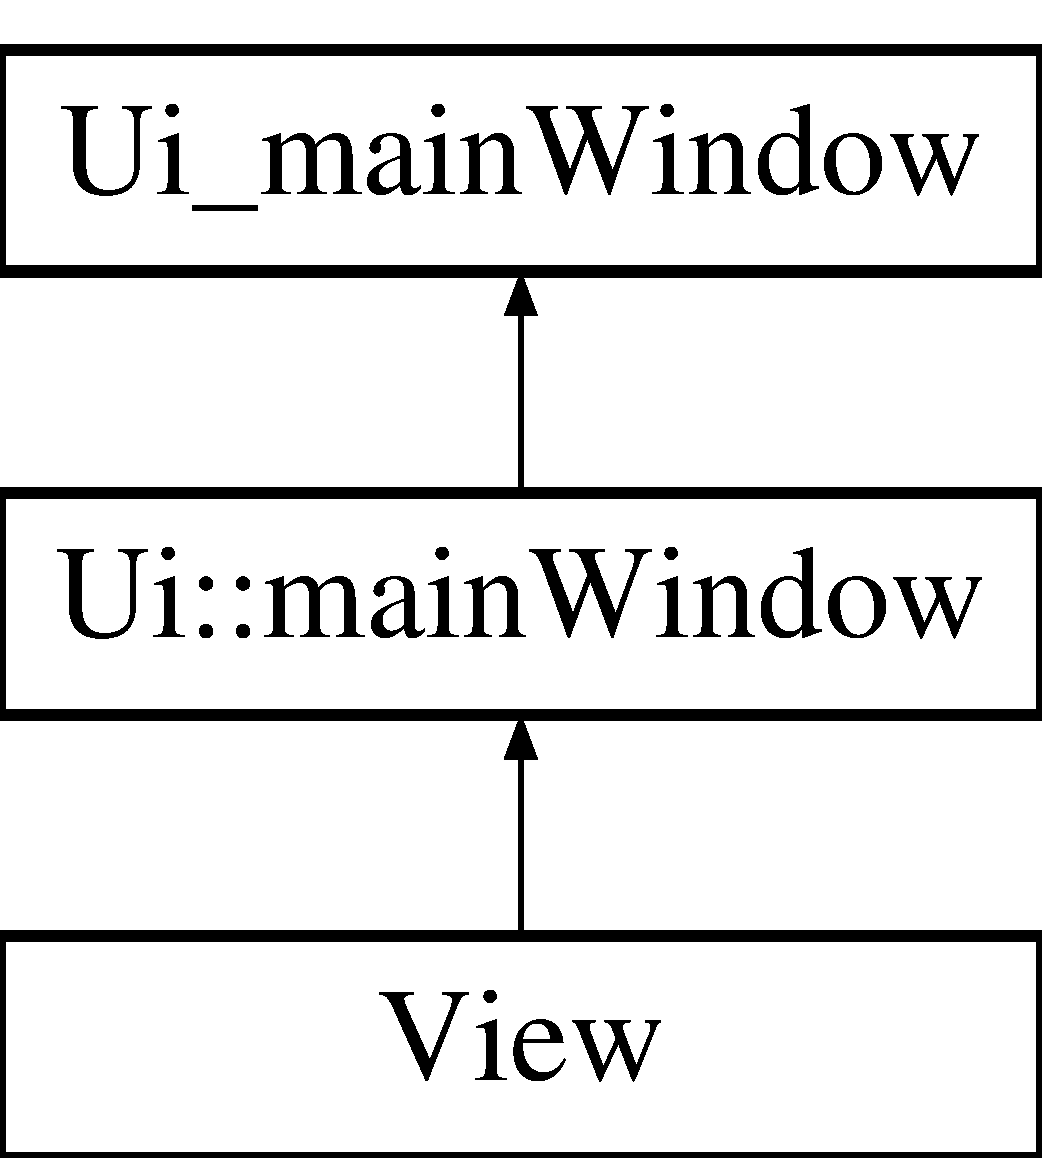
\includegraphics[height=3.000000cm]{class_ui__main_window}
\end{center}
\end{figure}
\subsection*{Public Member Functions}
\begin{DoxyCompactItemize}
\item 
void {\bf setup\-Ui} (Q\-Main\-Window $\ast$main\-Window)
\item 
void {\bf retranslate\-Ui} (Q\-Main\-Window $\ast$main\-Window)
\end{DoxyCompactItemize}
\subsection*{Public Attributes}
\begin{DoxyCompactItemize}
\item 
Q\-Action $\ast$ {\bf action\-Stop}
\item 
Q\-Action $\ast$ {\bf action\-Quit}
\item 
Q\-Action $\ast$ {\bf action\-New\-\_\-\-Course}
\item 
Q\-Action $\ast$ {\bf action\-Start}
\item 
Q\-Action $\ast$ {\bf action\-Schedule}
\item 
Q\-Widget $\ast$ {\bf central\-Widget}
\item 
Q\-Label $\ast$ {\bf label\-Welcome}
\item 
Q\-Label $\ast$ {\bf label\-Authors}
\item 
Q\-Push\-Button $\ast$ {\bf judge\-Button}
\item 
Q\-Push\-Button $\ast$ {\bf answer\-Button}
\item 
Q\-Push\-Button $\ast$ {\bf end\-Button}
\item 
Q\-Progress\-Bar $\ast$ {\bf progress\-Bar}
\item 
Q\-Label $\ast$ {\bf latwe}
\item 
Q\-Label $\ast$ {\bf trudne}
\item 
Q\-Slider $\ast$ {\bf vertical\-Slider}
\item 
Q\-Label $\ast$ {\bf question}
\item 
Q\-Text\-Edit $\ast$ {\bf answer\-Open\-Edit}
\item 
Q\-Push\-Button $\ast$ {\bf next\-Button}
\item 
Q\-Push\-Button $\ast$ {\bf back\-Button}
\item 
Q\-Label $\ast$ {\bf correct\-Answer}
\item 
Q\-Label $\ast$ {\bf value\-Judge}
\item 
Q\-Widget $\ast$ {\bf layout\-Widget}
\item 
Q\-Grid\-Layout $\ast$ {\bf grid\-Layout\-\_\-3}
\item 
Q\-Label $\ast$ {\bf answer\-Edit\-Close\-A}
\item 
Q\-Label $\ast$ {\bf answer\-Edit\-Close\-C}
\item 
Q\-Label $\ast$ {\bf answer\-Edit\-Close\-D}
\item 
Q\-Label $\ast$ {\bf answer\-Edit\-Close\-B}
\item 
Q\-Widget $\ast$ {\bf layout\-Widget1}
\item 
Q\-Grid\-Layout $\ast$ {\bf grid\-Layout}
\item 
Q\-Push\-Button $\ast$ {\bf a\-Button}
\item 
Q\-Push\-Button $\ast$ {\bf b\-Button}
\item 
Q\-Push\-Button $\ast$ {\bf c\-Button}
\item 
Q\-Push\-Button $\ast$ {\bf d\-Button}
\item 
Q\-Menu\-Bar $\ast$ {\bf menu\-Bar}
\item 
Q\-Menu $\ast$ {\bf menu\-File}
\item 
Q\-Menu $\ast$ {\bf menu\-Create}
\item 
Q\-Status\-Bar $\ast$ {\bf status\-Bar}
\end{DoxyCompactItemize}


\subsection{Member Function Documentation}
\index{Ui\-\_\-main\-Window@{Ui\-\_\-main\-Window}!retranslate\-Ui@{retranslate\-Ui}}
\index{retranslate\-Ui@{retranslate\-Ui}!Ui_mainWindow@{Ui\-\_\-main\-Window}}
\subsubsection[{retranslate\-Ui}]{\setlength{\rightskip}{0pt plus 5cm}void Ui\-\_\-main\-Window\-::retranslate\-Ui (
\begin{DoxyParamCaption}
\item[{Q\-Main\-Window $\ast$}]{main\-Window}
\end{DoxyParamCaption}
)\hspace{0.3cm}{\ttfamily [inline]}}\label{class_ui__main_window_a19d8fdf41c89c4e126c91765c5909d0e}
\index{Ui\-\_\-main\-Window@{Ui\-\_\-main\-Window}!setup\-Ui@{setup\-Ui}}
\index{setup\-Ui@{setup\-Ui}!Ui_mainWindow@{Ui\-\_\-main\-Window}}
\subsubsection[{setup\-Ui}]{\setlength{\rightskip}{0pt plus 5cm}void Ui\-\_\-main\-Window\-::setup\-Ui (
\begin{DoxyParamCaption}
\item[{Q\-Main\-Window $\ast$}]{main\-Window}
\end{DoxyParamCaption}
)\hspace{0.3cm}{\ttfamily [inline]}}\label{class_ui__main_window_ae7d1841a86020e8a4c12beb958596629}


\subsection{Member Data Documentation}
\index{Ui\-\_\-main\-Window@{Ui\-\_\-main\-Window}!a\-Button@{a\-Button}}
\index{a\-Button@{a\-Button}!Ui_mainWindow@{Ui\-\_\-main\-Window}}
\subsubsection[{a\-Button}]{\setlength{\rightskip}{0pt plus 5cm}Q\-Push\-Button$\ast$ Ui\-\_\-main\-Window\-::a\-Button}\label{class_ui__main_window_aa39f64ff1636e3c77b787abb4a3968f1}
\index{Ui\-\_\-main\-Window@{Ui\-\_\-main\-Window}!action\-New\-\_\-\-Course@{action\-New\-\_\-\-Course}}
\index{action\-New\-\_\-\-Course@{action\-New\-\_\-\-Course}!Ui_mainWindow@{Ui\-\_\-main\-Window}}
\subsubsection[{action\-New\-\_\-\-Course}]{\setlength{\rightskip}{0pt plus 5cm}Q\-Action$\ast$ Ui\-\_\-main\-Window\-::action\-New\-\_\-\-Course}\label{class_ui__main_window_af2a473d3eb9141ab0777a651e3e2d5fc}
\index{Ui\-\_\-main\-Window@{Ui\-\_\-main\-Window}!action\-Quit@{action\-Quit}}
\index{action\-Quit@{action\-Quit}!Ui_mainWindow@{Ui\-\_\-main\-Window}}
\subsubsection[{action\-Quit}]{\setlength{\rightskip}{0pt plus 5cm}Q\-Action$\ast$ Ui\-\_\-main\-Window\-::action\-Quit}\label{class_ui__main_window_ab08dd5b3c54c0f5f27e0d010c2d63e32}
\index{Ui\-\_\-main\-Window@{Ui\-\_\-main\-Window}!action\-Schedule@{action\-Schedule}}
\index{action\-Schedule@{action\-Schedule}!Ui_mainWindow@{Ui\-\_\-main\-Window}}
\subsubsection[{action\-Schedule}]{\setlength{\rightskip}{0pt plus 5cm}Q\-Action$\ast$ Ui\-\_\-main\-Window\-::action\-Schedule}\label{class_ui__main_window_a508d543f58f7184acf2aab685fe41783}
\index{Ui\-\_\-main\-Window@{Ui\-\_\-main\-Window}!action\-Start@{action\-Start}}
\index{action\-Start@{action\-Start}!Ui_mainWindow@{Ui\-\_\-main\-Window}}
\subsubsection[{action\-Start}]{\setlength{\rightskip}{0pt plus 5cm}Q\-Action$\ast$ Ui\-\_\-main\-Window\-::action\-Start}\label{class_ui__main_window_a1f7f6c45e3437a1c2de4d258329a6312}
\index{Ui\-\_\-main\-Window@{Ui\-\_\-main\-Window}!action\-Stop@{action\-Stop}}
\index{action\-Stop@{action\-Stop}!Ui_mainWindow@{Ui\-\_\-main\-Window}}
\subsubsection[{action\-Stop}]{\setlength{\rightskip}{0pt plus 5cm}Q\-Action$\ast$ Ui\-\_\-main\-Window\-::action\-Stop}\label{class_ui__main_window_a36c3f6068aa746a1536ab9f90e4a13fd}
\index{Ui\-\_\-main\-Window@{Ui\-\_\-main\-Window}!answer\-Button@{answer\-Button}}
\index{answer\-Button@{answer\-Button}!Ui_mainWindow@{Ui\-\_\-main\-Window}}
\subsubsection[{answer\-Button}]{\setlength{\rightskip}{0pt plus 5cm}Q\-Push\-Button$\ast$ Ui\-\_\-main\-Window\-::answer\-Button}\label{class_ui__main_window_a65ce4717df0c62846dd41ca14cd34acc}
\index{Ui\-\_\-main\-Window@{Ui\-\_\-main\-Window}!answer\-Edit\-Close\-A@{answer\-Edit\-Close\-A}}
\index{answer\-Edit\-Close\-A@{answer\-Edit\-Close\-A}!Ui_mainWindow@{Ui\-\_\-main\-Window}}
\subsubsection[{answer\-Edit\-Close\-A}]{\setlength{\rightskip}{0pt plus 5cm}Q\-Label$\ast$ Ui\-\_\-main\-Window\-::answer\-Edit\-Close\-A}\label{class_ui__main_window_a0d8a22bc3eb7df1c513c1ea5cea7e486}
\index{Ui\-\_\-main\-Window@{Ui\-\_\-main\-Window}!answer\-Edit\-Close\-B@{answer\-Edit\-Close\-B}}
\index{answer\-Edit\-Close\-B@{answer\-Edit\-Close\-B}!Ui_mainWindow@{Ui\-\_\-main\-Window}}
\subsubsection[{answer\-Edit\-Close\-B}]{\setlength{\rightskip}{0pt plus 5cm}Q\-Label$\ast$ Ui\-\_\-main\-Window\-::answer\-Edit\-Close\-B}\label{class_ui__main_window_a2abb93b91f1eb9bf9a398870d1736077}
\index{Ui\-\_\-main\-Window@{Ui\-\_\-main\-Window}!answer\-Edit\-Close\-C@{answer\-Edit\-Close\-C}}
\index{answer\-Edit\-Close\-C@{answer\-Edit\-Close\-C}!Ui_mainWindow@{Ui\-\_\-main\-Window}}
\subsubsection[{answer\-Edit\-Close\-C}]{\setlength{\rightskip}{0pt plus 5cm}Q\-Label$\ast$ Ui\-\_\-main\-Window\-::answer\-Edit\-Close\-C}\label{class_ui__main_window_ac4da7351cb1588c5b88630f855d3992f}
\index{Ui\-\_\-main\-Window@{Ui\-\_\-main\-Window}!answer\-Edit\-Close\-D@{answer\-Edit\-Close\-D}}
\index{answer\-Edit\-Close\-D@{answer\-Edit\-Close\-D}!Ui_mainWindow@{Ui\-\_\-main\-Window}}
\subsubsection[{answer\-Edit\-Close\-D}]{\setlength{\rightskip}{0pt plus 5cm}Q\-Label$\ast$ Ui\-\_\-main\-Window\-::answer\-Edit\-Close\-D}\label{class_ui__main_window_ab5951185d46422d1838f5eb2ead9f8b1}
\index{Ui\-\_\-main\-Window@{Ui\-\_\-main\-Window}!answer\-Open\-Edit@{answer\-Open\-Edit}}
\index{answer\-Open\-Edit@{answer\-Open\-Edit}!Ui_mainWindow@{Ui\-\_\-main\-Window}}
\subsubsection[{answer\-Open\-Edit}]{\setlength{\rightskip}{0pt plus 5cm}Q\-Text\-Edit$\ast$ Ui\-\_\-main\-Window\-::answer\-Open\-Edit}\label{class_ui__main_window_acfd58090bd951a46fd3311281ea579af}
\index{Ui\-\_\-main\-Window@{Ui\-\_\-main\-Window}!back\-Button@{back\-Button}}
\index{back\-Button@{back\-Button}!Ui_mainWindow@{Ui\-\_\-main\-Window}}
\subsubsection[{back\-Button}]{\setlength{\rightskip}{0pt plus 5cm}Q\-Push\-Button$\ast$ Ui\-\_\-main\-Window\-::back\-Button}\label{class_ui__main_window_ad689a113fe1d2e626aaa21911cffc34c}
\index{Ui\-\_\-main\-Window@{Ui\-\_\-main\-Window}!b\-Button@{b\-Button}}
\index{b\-Button@{b\-Button}!Ui_mainWindow@{Ui\-\_\-main\-Window}}
\subsubsection[{b\-Button}]{\setlength{\rightskip}{0pt plus 5cm}Q\-Push\-Button$\ast$ Ui\-\_\-main\-Window\-::b\-Button}\label{class_ui__main_window_a1af97b2c29cc5bf9d84cbe4dbb377506}
\index{Ui\-\_\-main\-Window@{Ui\-\_\-main\-Window}!c\-Button@{c\-Button}}
\index{c\-Button@{c\-Button}!Ui_mainWindow@{Ui\-\_\-main\-Window}}
\subsubsection[{c\-Button}]{\setlength{\rightskip}{0pt plus 5cm}Q\-Push\-Button$\ast$ Ui\-\_\-main\-Window\-::c\-Button}\label{class_ui__main_window_adb2b0c90de4b0ead7efc16f6d11d2b69}
\index{Ui\-\_\-main\-Window@{Ui\-\_\-main\-Window}!central\-Widget@{central\-Widget}}
\index{central\-Widget@{central\-Widget}!Ui_mainWindow@{Ui\-\_\-main\-Window}}
\subsubsection[{central\-Widget}]{\setlength{\rightskip}{0pt plus 5cm}Q\-Widget$\ast$ Ui\-\_\-main\-Window\-::central\-Widget}\label{class_ui__main_window_aee46367bf469e64ab25cc11ed32ea83a}
\index{Ui\-\_\-main\-Window@{Ui\-\_\-main\-Window}!correct\-Answer@{correct\-Answer}}
\index{correct\-Answer@{correct\-Answer}!Ui_mainWindow@{Ui\-\_\-main\-Window}}
\subsubsection[{correct\-Answer}]{\setlength{\rightskip}{0pt plus 5cm}Q\-Label$\ast$ Ui\-\_\-main\-Window\-::correct\-Answer}\label{class_ui__main_window_ab1e4fe666d2253bc08ed9932a98ffddb}
\index{Ui\-\_\-main\-Window@{Ui\-\_\-main\-Window}!d\-Button@{d\-Button}}
\index{d\-Button@{d\-Button}!Ui_mainWindow@{Ui\-\_\-main\-Window}}
\subsubsection[{d\-Button}]{\setlength{\rightskip}{0pt plus 5cm}Q\-Push\-Button$\ast$ Ui\-\_\-main\-Window\-::d\-Button}\label{class_ui__main_window_aadde7c28fabd0fd3c0e48bef807cb0f5}
\index{Ui\-\_\-main\-Window@{Ui\-\_\-main\-Window}!end\-Button@{end\-Button}}
\index{end\-Button@{end\-Button}!Ui_mainWindow@{Ui\-\_\-main\-Window}}
\subsubsection[{end\-Button}]{\setlength{\rightskip}{0pt plus 5cm}Q\-Push\-Button$\ast$ Ui\-\_\-main\-Window\-::end\-Button}\label{class_ui__main_window_aabdb91a0a8edaddaae247d5d3d86e79c}
\index{Ui\-\_\-main\-Window@{Ui\-\_\-main\-Window}!grid\-Layout@{grid\-Layout}}
\index{grid\-Layout@{grid\-Layout}!Ui_mainWindow@{Ui\-\_\-main\-Window}}
\subsubsection[{grid\-Layout}]{\setlength{\rightskip}{0pt plus 5cm}Q\-Grid\-Layout$\ast$ Ui\-\_\-main\-Window\-::grid\-Layout}\label{class_ui__main_window_a276f7f08d8b9667bc235b5d794fc2425}
\index{Ui\-\_\-main\-Window@{Ui\-\_\-main\-Window}!grid\-Layout\-\_\-3@{grid\-Layout\-\_\-3}}
\index{grid\-Layout\-\_\-3@{grid\-Layout\-\_\-3}!Ui_mainWindow@{Ui\-\_\-main\-Window}}
\subsubsection[{grid\-Layout\-\_\-3}]{\setlength{\rightskip}{0pt plus 5cm}Q\-Grid\-Layout$\ast$ Ui\-\_\-main\-Window\-::grid\-Layout\-\_\-3}\label{class_ui__main_window_a5584701b1c53621380c54a2aaaf7ce34}
\index{Ui\-\_\-main\-Window@{Ui\-\_\-main\-Window}!judge\-Button@{judge\-Button}}
\index{judge\-Button@{judge\-Button}!Ui_mainWindow@{Ui\-\_\-main\-Window}}
\subsubsection[{judge\-Button}]{\setlength{\rightskip}{0pt plus 5cm}Q\-Push\-Button$\ast$ Ui\-\_\-main\-Window\-::judge\-Button}\label{class_ui__main_window_a1cefef2686e09971dde44e29206bfb7d}
\index{Ui\-\_\-main\-Window@{Ui\-\_\-main\-Window}!label\-Authors@{label\-Authors}}
\index{label\-Authors@{label\-Authors}!Ui_mainWindow@{Ui\-\_\-main\-Window}}
\subsubsection[{label\-Authors}]{\setlength{\rightskip}{0pt plus 5cm}Q\-Label$\ast$ Ui\-\_\-main\-Window\-::label\-Authors}\label{class_ui__main_window_acd6a34e6270e76547944b70bca92096e}
\index{Ui\-\_\-main\-Window@{Ui\-\_\-main\-Window}!label\-Welcome@{label\-Welcome}}
\index{label\-Welcome@{label\-Welcome}!Ui_mainWindow@{Ui\-\_\-main\-Window}}
\subsubsection[{label\-Welcome}]{\setlength{\rightskip}{0pt plus 5cm}Q\-Label$\ast$ Ui\-\_\-main\-Window\-::label\-Welcome}\label{class_ui__main_window_a093c520b58229f0c331d64c361cec8cd}
\index{Ui\-\_\-main\-Window@{Ui\-\_\-main\-Window}!latwe@{latwe}}
\index{latwe@{latwe}!Ui_mainWindow@{Ui\-\_\-main\-Window}}
\subsubsection[{latwe}]{\setlength{\rightskip}{0pt plus 5cm}Q\-Label$\ast$ Ui\-\_\-main\-Window\-::latwe}\label{class_ui__main_window_ab5cd3b2b3c6e05b4c6576323dd7245bb}
\index{Ui\-\_\-main\-Window@{Ui\-\_\-main\-Window}!layout\-Widget@{layout\-Widget}}
\index{layout\-Widget@{layout\-Widget}!Ui_mainWindow@{Ui\-\_\-main\-Window}}
\subsubsection[{layout\-Widget}]{\setlength{\rightskip}{0pt plus 5cm}Q\-Widget$\ast$ Ui\-\_\-main\-Window\-::layout\-Widget}\label{class_ui__main_window_aa24b207160749f7ba841d36ca5f913de}
\index{Ui\-\_\-main\-Window@{Ui\-\_\-main\-Window}!layout\-Widget1@{layout\-Widget1}}
\index{layout\-Widget1@{layout\-Widget1}!Ui_mainWindow@{Ui\-\_\-main\-Window}}
\subsubsection[{layout\-Widget1}]{\setlength{\rightskip}{0pt plus 5cm}Q\-Widget$\ast$ Ui\-\_\-main\-Window\-::layout\-Widget1}\label{class_ui__main_window_a21e62b1c9527b4e9ccfdc87a108a5a4a}
\index{Ui\-\_\-main\-Window@{Ui\-\_\-main\-Window}!menu\-Bar@{menu\-Bar}}
\index{menu\-Bar@{menu\-Bar}!Ui_mainWindow@{Ui\-\_\-main\-Window}}
\subsubsection[{menu\-Bar}]{\setlength{\rightskip}{0pt plus 5cm}Q\-Menu\-Bar$\ast$ Ui\-\_\-main\-Window\-::menu\-Bar}\label{class_ui__main_window_a68c23188650ef87ba2974e81ada5be37}
\index{Ui\-\_\-main\-Window@{Ui\-\_\-main\-Window}!menu\-Create@{menu\-Create}}
\index{menu\-Create@{menu\-Create}!Ui_mainWindow@{Ui\-\_\-main\-Window}}
\subsubsection[{menu\-Create}]{\setlength{\rightskip}{0pt plus 5cm}Q\-Menu$\ast$ Ui\-\_\-main\-Window\-::menu\-Create}\label{class_ui__main_window_a55249892134f65b4a6332c3b36df6d04}
\index{Ui\-\_\-main\-Window@{Ui\-\_\-main\-Window}!menu\-File@{menu\-File}}
\index{menu\-File@{menu\-File}!Ui_mainWindow@{Ui\-\_\-main\-Window}}
\subsubsection[{menu\-File}]{\setlength{\rightskip}{0pt plus 5cm}Q\-Menu$\ast$ Ui\-\_\-main\-Window\-::menu\-File}\label{class_ui__main_window_a4d68ee90d56a865e62aa7f52200e00c4}
\index{Ui\-\_\-main\-Window@{Ui\-\_\-main\-Window}!next\-Button@{next\-Button}}
\index{next\-Button@{next\-Button}!Ui_mainWindow@{Ui\-\_\-main\-Window}}
\subsubsection[{next\-Button}]{\setlength{\rightskip}{0pt plus 5cm}Q\-Push\-Button$\ast$ Ui\-\_\-main\-Window\-::next\-Button}\label{class_ui__main_window_a42510177582e05956f040d578fbf5745}
\index{Ui\-\_\-main\-Window@{Ui\-\_\-main\-Window}!progress\-Bar@{progress\-Bar}}
\index{progress\-Bar@{progress\-Bar}!Ui_mainWindow@{Ui\-\_\-main\-Window}}
\subsubsection[{progress\-Bar}]{\setlength{\rightskip}{0pt plus 5cm}Q\-Progress\-Bar$\ast$ Ui\-\_\-main\-Window\-::progress\-Bar}\label{class_ui__main_window_ac1a67dbb39679aca497a2c58d25438e2}
\index{Ui\-\_\-main\-Window@{Ui\-\_\-main\-Window}!question@{question}}
\index{question@{question}!Ui_mainWindow@{Ui\-\_\-main\-Window}}
\subsubsection[{question}]{\setlength{\rightskip}{0pt plus 5cm}Q\-Label$\ast$ Ui\-\_\-main\-Window\-::question}\label{class_ui__main_window_a659a1fc6efb01e3325b67bf200d72a65}
\index{Ui\-\_\-main\-Window@{Ui\-\_\-main\-Window}!status\-Bar@{status\-Bar}}
\index{status\-Bar@{status\-Bar}!Ui_mainWindow@{Ui\-\_\-main\-Window}}
\subsubsection[{status\-Bar}]{\setlength{\rightskip}{0pt plus 5cm}Q\-Status\-Bar$\ast$ Ui\-\_\-main\-Window\-::status\-Bar}\label{class_ui__main_window_a520571ba95734c931586c582134d0219}
\index{Ui\-\_\-main\-Window@{Ui\-\_\-main\-Window}!trudne@{trudne}}
\index{trudne@{trudne}!Ui_mainWindow@{Ui\-\_\-main\-Window}}
\subsubsection[{trudne}]{\setlength{\rightskip}{0pt plus 5cm}Q\-Label$\ast$ Ui\-\_\-main\-Window\-::trudne}\label{class_ui__main_window_ad4fa099b7852f9a0f7778e61ddf0077f}
\index{Ui\-\_\-main\-Window@{Ui\-\_\-main\-Window}!value\-Judge@{value\-Judge}}
\index{value\-Judge@{value\-Judge}!Ui_mainWindow@{Ui\-\_\-main\-Window}}
\subsubsection[{value\-Judge}]{\setlength{\rightskip}{0pt plus 5cm}Q\-Label$\ast$ Ui\-\_\-main\-Window\-::value\-Judge}\label{class_ui__main_window_a7d99246c2abf4185f0b2256f5ef0474d}
\index{Ui\-\_\-main\-Window@{Ui\-\_\-main\-Window}!vertical\-Slider@{vertical\-Slider}}
\index{vertical\-Slider@{vertical\-Slider}!Ui_mainWindow@{Ui\-\_\-main\-Window}}
\subsubsection[{vertical\-Slider}]{\setlength{\rightskip}{0pt plus 5cm}Q\-Slider$\ast$ Ui\-\_\-main\-Window\-::vertical\-Slider}\label{class_ui__main_window_a1d755944d8ca6e6d86a9a92ac05bbb77}


The documentation for this class was generated from the following file\-:\begin{DoxyCompactItemize}
\item 
Projekt\-Z\-P\-R/\-Generated\-Files/{\bf ui\-\_\-projektzpr.\-h}\end{DoxyCompactItemize}

\section{Ui\-\_\-\-Schedule Class Reference}
\label{class_ui___schedule}\index{Ui\-\_\-\-Schedule@{Ui\-\_\-\-Schedule}}


{\ttfamily \#include $<$ui\-\_\-schedule.\-h$>$}

Inheritance diagram for Ui\-\_\-\-Schedule\-:\begin{figure}[H]
\begin{center}
\leavevmode
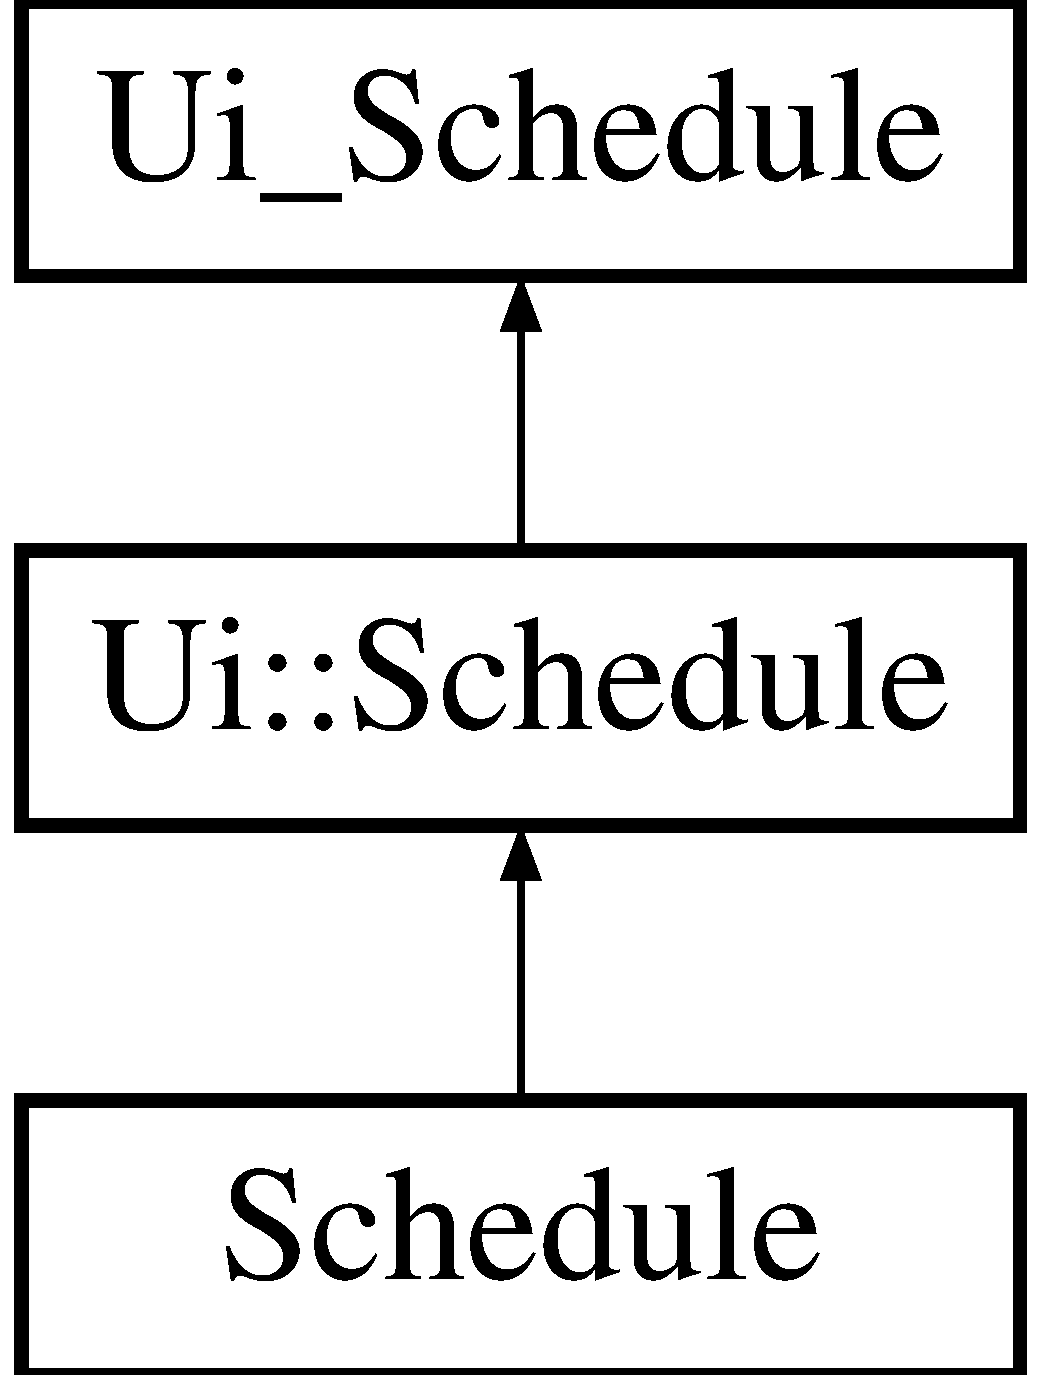
\includegraphics[height=3.000000cm]{class_ui___schedule}
\end{center}
\end{figure}
\subsection*{Public Member Functions}
\begin{DoxyCompactItemize}
\item 
void {\bf setup\-Ui} (Q\-Widget $\ast${\bf Schedule})
\item 
void {\bf retranslate\-Ui} (Q\-Widget $\ast${\bf Schedule})
\end{DoxyCompactItemize}
\subsection*{Public Attributes}
\begin{DoxyCompactItemize}
\item 
Q\-List\-Widget $\ast$ {\bf courses\-List}
\item 
Q\-Label $\ast$ {\bf label}
\item 
Q\-Label $\ast$ {\bf label\-\_\-2}
\item 
Q\-List\-Widget $\ast$ {\bf list\-Later}
\end{DoxyCompactItemize}


\subsection{Member Function Documentation}
\index{Ui\-\_\-\-Schedule@{Ui\-\_\-\-Schedule}!retranslate\-Ui@{retranslate\-Ui}}
\index{retranslate\-Ui@{retranslate\-Ui}!Ui_Schedule@{Ui\-\_\-\-Schedule}}
\subsubsection[{retranslate\-Ui}]{\setlength{\rightskip}{0pt plus 5cm}void Ui\-\_\-\-Schedule\-::retranslate\-Ui (
\begin{DoxyParamCaption}
\item[{Q\-Widget $\ast$}]{Schedule}
\end{DoxyParamCaption}
)\hspace{0.3cm}{\ttfamily [inline]}}\label{class_ui___schedule_a75c8b4051d671dfa4fac0170687ed012}
\index{Ui\-\_\-\-Schedule@{Ui\-\_\-\-Schedule}!setup\-Ui@{setup\-Ui}}
\index{setup\-Ui@{setup\-Ui}!Ui_Schedule@{Ui\-\_\-\-Schedule}}
\subsubsection[{setup\-Ui}]{\setlength{\rightskip}{0pt plus 5cm}void Ui\-\_\-\-Schedule\-::setup\-Ui (
\begin{DoxyParamCaption}
\item[{Q\-Widget $\ast$}]{Schedule}
\end{DoxyParamCaption}
)\hspace{0.3cm}{\ttfamily [inline]}}\label{class_ui___schedule_af4c95e0aa93455dcee2afc584939d70b}


\subsection{Member Data Documentation}
\index{Ui\-\_\-\-Schedule@{Ui\-\_\-\-Schedule}!courses\-List@{courses\-List}}
\index{courses\-List@{courses\-List}!Ui_Schedule@{Ui\-\_\-\-Schedule}}
\subsubsection[{courses\-List}]{\setlength{\rightskip}{0pt plus 5cm}Q\-List\-Widget$\ast$ Ui\-\_\-\-Schedule\-::courses\-List}\label{class_ui___schedule_adb6ec53c84ae6c830b1384bda7bd306c}
\index{Ui\-\_\-\-Schedule@{Ui\-\_\-\-Schedule}!label@{label}}
\index{label@{label}!Ui_Schedule@{Ui\-\_\-\-Schedule}}
\subsubsection[{label}]{\setlength{\rightskip}{0pt plus 5cm}Q\-Label$\ast$ Ui\-\_\-\-Schedule\-::label}\label{class_ui___schedule_a05c62db33e8f9fac657fb5294440377c}
\index{Ui\-\_\-\-Schedule@{Ui\-\_\-\-Schedule}!label\-\_\-2@{label\-\_\-2}}
\index{label\-\_\-2@{label\-\_\-2}!Ui_Schedule@{Ui\-\_\-\-Schedule}}
\subsubsection[{label\-\_\-2}]{\setlength{\rightskip}{0pt plus 5cm}Q\-Label$\ast$ Ui\-\_\-\-Schedule\-::label\-\_\-2}\label{class_ui___schedule_a90b62e30c313c55006fec42757b0784d}
\index{Ui\-\_\-\-Schedule@{Ui\-\_\-\-Schedule}!list\-Later@{list\-Later}}
\index{list\-Later@{list\-Later}!Ui_Schedule@{Ui\-\_\-\-Schedule}}
\subsubsection[{list\-Later}]{\setlength{\rightskip}{0pt plus 5cm}Q\-List\-Widget$\ast$ Ui\-\_\-\-Schedule\-::list\-Later}\label{class_ui___schedule_a895c0ee7384da0a0c11711e66864e778}


The documentation for this class was generated from the following file\-:\begin{DoxyCompactItemize}
\item 
Projekt\-Z\-P\-R/\-Generated\-Files/{\bf ui\-\_\-schedule.\-h}\end{DoxyCompactItemize}

\section{Ui\-\_\-\-Start\-Menu Class Reference}
\label{class_ui___start_menu}\index{Ui\-\_\-\-Start\-Menu@{Ui\-\_\-\-Start\-Menu}}


{\ttfamily \#include $<$ui\-\_\-startmenu.\-h$>$}

Inheritance diagram for Ui\-\_\-\-Start\-Menu\-:\begin{figure}[H]
\begin{center}
\leavevmode
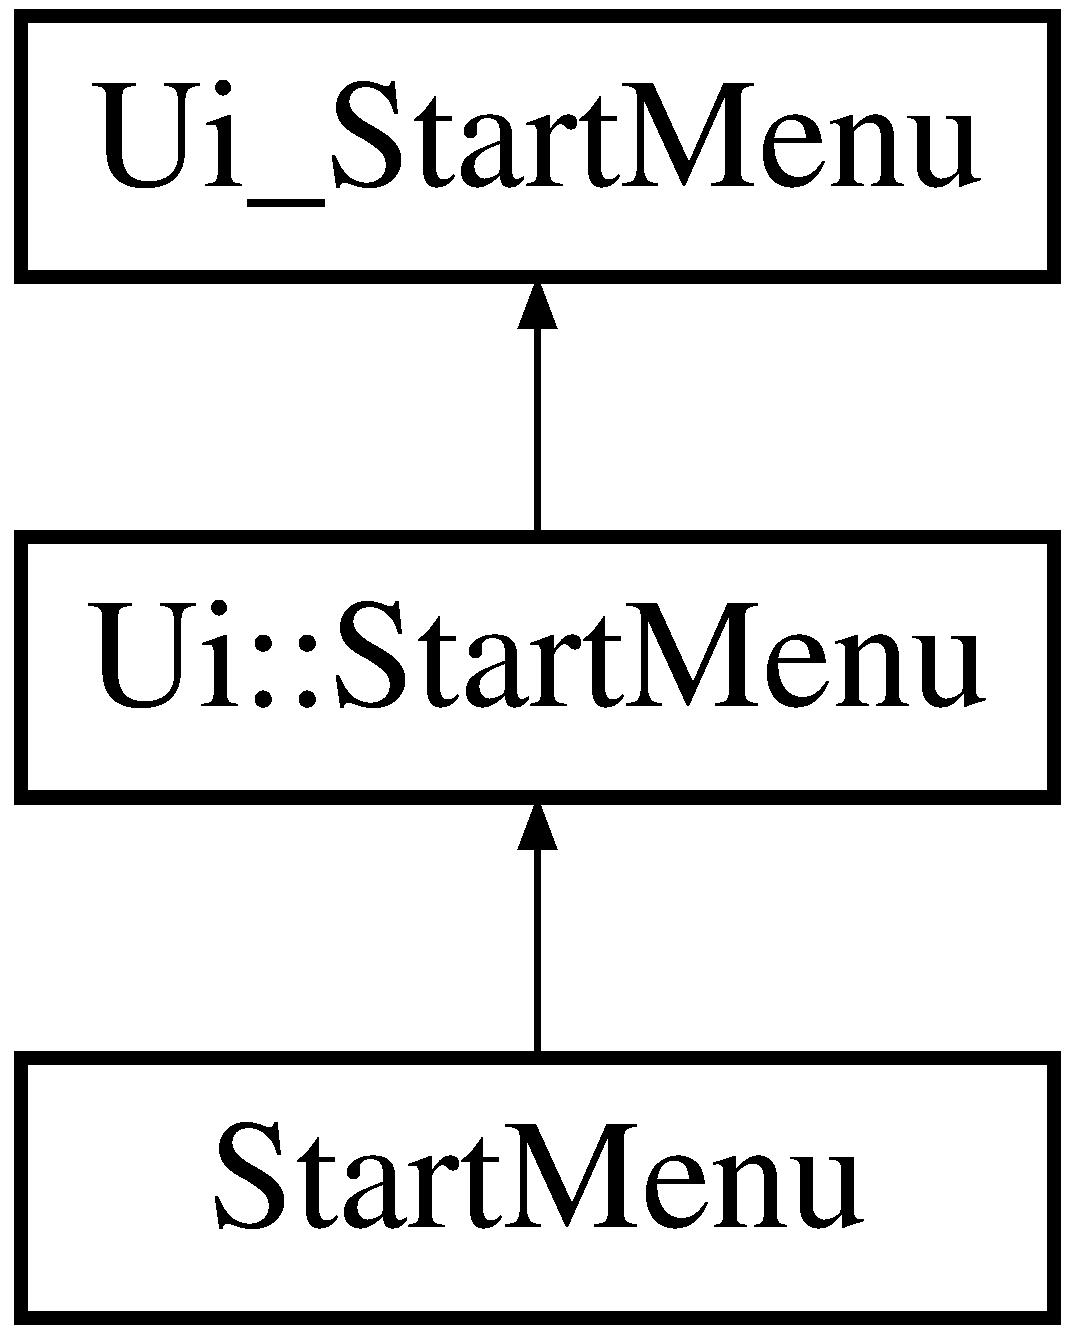
\includegraphics[height=3.000000cm]{class_ui___start_menu}
\end{center}
\end{figure}
\subsection*{Public Member Functions}
\begin{DoxyCompactItemize}
\item 
void {\bf setup\-Ui} (Q\-Widget $\ast${\bf Start\-Menu})
\item 
void {\bf retranslate\-Ui} (Q\-Widget $\ast${\bf Start\-Menu})
\end{DoxyCompactItemize}
\subsection*{Public Attributes}
\begin{DoxyCompactItemize}
\item 
Q\-Label $\ast$ {\bf label}
\item 
Q\-Widget $\ast$ {\bf layout\-Widget}
\item 
Q\-V\-Box\-Layout $\ast$ {\bf vertical\-Layout}
\item 
Q\-List\-Widget $\ast$ {\bf courses\-List}
\item 
Q\-H\-Box\-Layout $\ast$ {\bf horizontal\-Layout}
\item 
Q\-Push\-Button $\ast$ {\bf choose}
\item 
Q\-Push\-Button $\ast$ {\bf delete\-Button}
\item 
Q\-Push\-Button $\ast$ {\bf continue\-Button}
\end{DoxyCompactItemize}


\subsection{Member Function Documentation}
\index{Ui\-\_\-\-Start\-Menu@{Ui\-\_\-\-Start\-Menu}!retranslate\-Ui@{retranslate\-Ui}}
\index{retranslate\-Ui@{retranslate\-Ui}!Ui_StartMenu@{Ui\-\_\-\-Start\-Menu}}
\subsubsection[{retranslate\-Ui}]{\setlength{\rightskip}{0pt plus 5cm}void Ui\-\_\-\-Start\-Menu\-::retranslate\-Ui (
\begin{DoxyParamCaption}
\item[{Q\-Widget $\ast$}]{Start\-Menu}
\end{DoxyParamCaption}
)\hspace{0.3cm}{\ttfamily [inline]}}\label{class_ui___start_menu_ae47755e0869e14612fb4f913fc05d40a}
\index{Ui\-\_\-\-Start\-Menu@{Ui\-\_\-\-Start\-Menu}!setup\-Ui@{setup\-Ui}}
\index{setup\-Ui@{setup\-Ui}!Ui_StartMenu@{Ui\-\_\-\-Start\-Menu}}
\subsubsection[{setup\-Ui}]{\setlength{\rightskip}{0pt plus 5cm}void Ui\-\_\-\-Start\-Menu\-::setup\-Ui (
\begin{DoxyParamCaption}
\item[{Q\-Widget $\ast$}]{Start\-Menu}
\end{DoxyParamCaption}
)\hspace{0.3cm}{\ttfamily [inline]}}\label{class_ui___start_menu_a22316c658efac7bcae6ed2bc3df2a9d1}


\subsection{Member Data Documentation}
\index{Ui\-\_\-\-Start\-Menu@{Ui\-\_\-\-Start\-Menu}!choose@{choose}}
\index{choose@{choose}!Ui_StartMenu@{Ui\-\_\-\-Start\-Menu}}
\subsubsection[{choose}]{\setlength{\rightskip}{0pt plus 5cm}Q\-Push\-Button$\ast$ Ui\-\_\-\-Start\-Menu\-::choose}\label{class_ui___start_menu_a00b9f140128571461171c44c6b5fbade}
\index{Ui\-\_\-\-Start\-Menu@{Ui\-\_\-\-Start\-Menu}!continue\-Button@{continue\-Button}}
\index{continue\-Button@{continue\-Button}!Ui_StartMenu@{Ui\-\_\-\-Start\-Menu}}
\subsubsection[{continue\-Button}]{\setlength{\rightskip}{0pt plus 5cm}Q\-Push\-Button$\ast$ Ui\-\_\-\-Start\-Menu\-::continue\-Button}\label{class_ui___start_menu_a28cd0da76e6ce0824a19a84dfee06c0c}
\index{Ui\-\_\-\-Start\-Menu@{Ui\-\_\-\-Start\-Menu}!courses\-List@{courses\-List}}
\index{courses\-List@{courses\-List}!Ui_StartMenu@{Ui\-\_\-\-Start\-Menu}}
\subsubsection[{courses\-List}]{\setlength{\rightskip}{0pt plus 5cm}Q\-List\-Widget$\ast$ Ui\-\_\-\-Start\-Menu\-::courses\-List}\label{class_ui___start_menu_a0cc39b7f7a87e34d77ca1d5986da2323}
\index{Ui\-\_\-\-Start\-Menu@{Ui\-\_\-\-Start\-Menu}!delete\-Button@{delete\-Button}}
\index{delete\-Button@{delete\-Button}!Ui_StartMenu@{Ui\-\_\-\-Start\-Menu}}
\subsubsection[{delete\-Button}]{\setlength{\rightskip}{0pt plus 5cm}Q\-Push\-Button$\ast$ Ui\-\_\-\-Start\-Menu\-::delete\-Button}\label{class_ui___start_menu_a7eef229054f1d64c61be975d3b7012e5}
\index{Ui\-\_\-\-Start\-Menu@{Ui\-\_\-\-Start\-Menu}!horizontal\-Layout@{horizontal\-Layout}}
\index{horizontal\-Layout@{horizontal\-Layout}!Ui_StartMenu@{Ui\-\_\-\-Start\-Menu}}
\subsubsection[{horizontal\-Layout}]{\setlength{\rightskip}{0pt plus 5cm}Q\-H\-Box\-Layout$\ast$ Ui\-\_\-\-Start\-Menu\-::horizontal\-Layout}\label{class_ui___start_menu_a247e8d0277873536c787ed5e2c038706}
\index{Ui\-\_\-\-Start\-Menu@{Ui\-\_\-\-Start\-Menu}!label@{label}}
\index{label@{label}!Ui_StartMenu@{Ui\-\_\-\-Start\-Menu}}
\subsubsection[{label}]{\setlength{\rightskip}{0pt plus 5cm}Q\-Label$\ast$ Ui\-\_\-\-Start\-Menu\-::label}\label{class_ui___start_menu_a274813cfd4f7ff42d483373ce1855d3d}
\index{Ui\-\_\-\-Start\-Menu@{Ui\-\_\-\-Start\-Menu}!layout\-Widget@{layout\-Widget}}
\index{layout\-Widget@{layout\-Widget}!Ui_StartMenu@{Ui\-\_\-\-Start\-Menu}}
\subsubsection[{layout\-Widget}]{\setlength{\rightskip}{0pt plus 5cm}Q\-Widget$\ast$ Ui\-\_\-\-Start\-Menu\-::layout\-Widget}\label{class_ui___start_menu_a158f8249c94edc210205f48212152feb}
\index{Ui\-\_\-\-Start\-Menu@{Ui\-\_\-\-Start\-Menu}!vertical\-Layout@{vertical\-Layout}}
\index{vertical\-Layout@{vertical\-Layout}!Ui_StartMenu@{Ui\-\_\-\-Start\-Menu}}
\subsubsection[{vertical\-Layout}]{\setlength{\rightskip}{0pt plus 5cm}Q\-V\-Box\-Layout$\ast$ Ui\-\_\-\-Start\-Menu\-::vertical\-Layout}\label{class_ui___start_menu_a64f359e686ba29742dab589010fd0fb0}


The documentation for this class was generated from the following file\-:\begin{DoxyCompactItemize}
\item 
Projekt\-Z\-P\-R/\-Generated\-Files/{\bf ui\-\_\-startmenu.\-h}\end{DoxyCompactItemize}

\section{Ui\-\_\-\-Statistic Class Reference}
\label{class_ui___statistic}\index{Ui\-\_\-\-Statistic@{Ui\-\_\-\-Statistic}}


{\ttfamily \#include $<$ui\-\_\-statistic.\-h$>$}

Inheritance diagram for Ui\-\_\-\-Statistic\-:\begin{figure}[H]
\begin{center}
\leavevmode
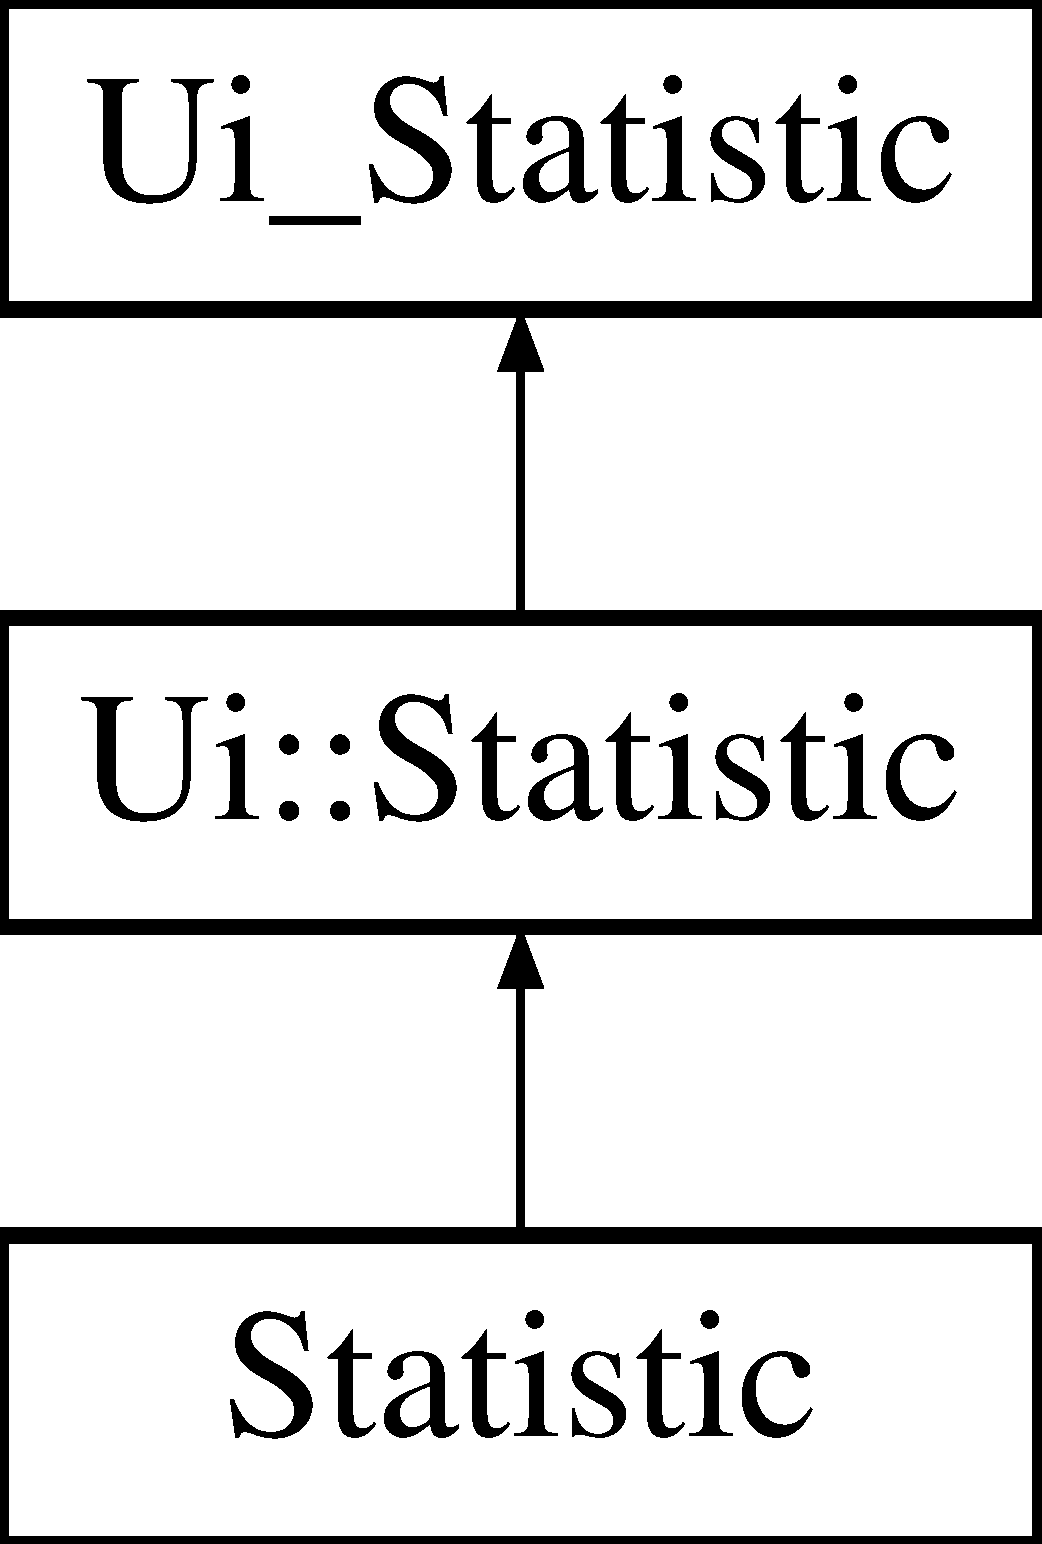
\includegraphics[height=3.000000cm]{class_ui___statistic}
\end{center}
\end{figure}
\subsection*{Public Member Functions}
\begin{DoxyCompactItemize}
\item 
void {\bf setup\-Ui} (Q\-Widget $\ast${\bf Statistic})
\item 
void {\bf retranslate\-Ui} (Q\-Widget $\ast${\bf Statistic})
\end{DoxyCompactItemize}
\subsection*{Public Attributes}
\begin{DoxyCompactItemize}
\item 
Q\-Label $\ast$ {\bf label\-Stats}
\end{DoxyCompactItemize}


\subsection{Member Function Documentation}
\index{Ui\-\_\-\-Statistic@{Ui\-\_\-\-Statistic}!retranslate\-Ui@{retranslate\-Ui}}
\index{retranslate\-Ui@{retranslate\-Ui}!Ui_Statistic@{Ui\-\_\-\-Statistic}}
\subsubsection[{retranslate\-Ui}]{\setlength{\rightskip}{0pt plus 5cm}void Ui\-\_\-\-Statistic\-::retranslate\-Ui (
\begin{DoxyParamCaption}
\item[{Q\-Widget $\ast$}]{Statistic}
\end{DoxyParamCaption}
)\hspace{0.3cm}{\ttfamily [inline]}}\label{class_ui___statistic_a2401b833be64523ee7b3305f64c9fddb}
\index{Ui\-\_\-\-Statistic@{Ui\-\_\-\-Statistic}!setup\-Ui@{setup\-Ui}}
\index{setup\-Ui@{setup\-Ui}!Ui_Statistic@{Ui\-\_\-\-Statistic}}
\subsubsection[{setup\-Ui}]{\setlength{\rightskip}{0pt plus 5cm}void Ui\-\_\-\-Statistic\-::setup\-Ui (
\begin{DoxyParamCaption}
\item[{Q\-Widget $\ast$}]{Statistic}
\end{DoxyParamCaption}
)\hspace{0.3cm}{\ttfamily [inline]}}\label{class_ui___statistic_a4fd1095b63b9fd5f8483692a268cdc49}


\subsection{Member Data Documentation}
\index{Ui\-\_\-\-Statistic@{Ui\-\_\-\-Statistic}!label\-Stats@{label\-Stats}}
\index{label\-Stats@{label\-Stats}!Ui_Statistic@{Ui\-\_\-\-Statistic}}
\subsubsection[{label\-Stats}]{\setlength{\rightskip}{0pt plus 5cm}Q\-Label$\ast$ Ui\-\_\-\-Statistic\-::label\-Stats}\label{class_ui___statistic_aa34c5e55269b165e9786771c5bc1ce26}


The documentation for this class was generated from the following file\-:\begin{DoxyCompactItemize}
\item 
Projekt\-Z\-P\-R/\-Generated\-Files/{\bf ui\-\_\-statistic.\-h}\end{DoxyCompactItemize}

\section{View Class Reference}
\label{class_view}\index{View@{View}}


{\ttfamily \#include $<$view.\-h$>$}

Inheritance diagram for View\-:\begin{figure}[H]
\begin{center}
\leavevmode
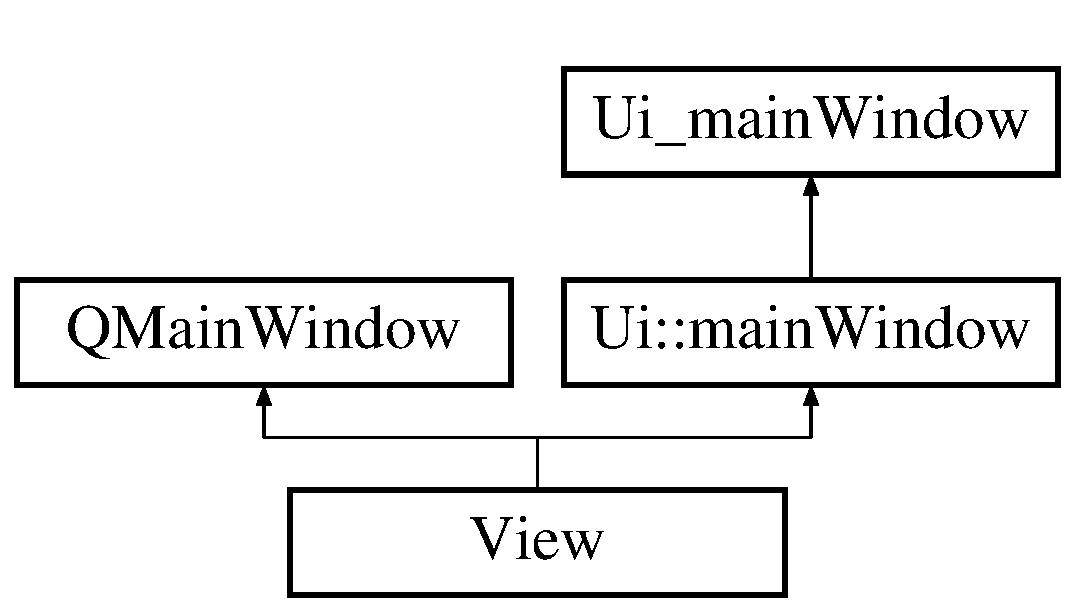
\includegraphics[height=3.000000cm]{class_view}
\end{center}
\end{figure}
\subsection*{Public Slots}
\begin{DoxyCompactItemize}
\item 
void {\bf enabled\-Main\-Win} ()
\begin{DoxyCompactList}\small\item\em set enable main window \end{DoxyCompactList}\item 
void {\bf show\-You} ()
\begin{DoxyCompactList}\small\item\em show main window \end{DoxyCompactList}\item 
void {\bf show\-Error} (std\-::string message)
\begin{DoxyCompactList}\small\item\em show warning message \end{DoxyCompactList}\item 
void {\bf show\-Question\-Card\-List} (vector$<$ {\bf P\-Qcard} $>$, std\-::string)
\begin{DoxyCompactList}\small\item\em set initial value and show first task \end{DoxyCompactList}\item 
void {\bf change\-Value\-Of\-Slider} (int)
\begin{DoxyCompactList}\small\item\em change judge\-Label when value of slider change \end{DoxyCompactList}\item 
void {\bf set\-Suggester\-Mark} (int)
\begin{DoxyCompactList}\small\item\em set suggested mark \end{DoxyCompactList}\end{DoxyCompactItemize}
\subsection*{Signals}
\begin{DoxyCompactItemize}
\item 
void {\bf set\-Current\-Task\-Next} (int id, std\-::string {\bf question}, std\-::string answer)
\begin{DoxyCompactList}\small\item\em Emit during creating new course to save current task, when we go to next task. It contains task id, question and answer. \end{DoxyCompactList}\item 
void {\bf set\-Current\-Task\-Back} (int id, std\-::string {\bf question}, std\-::string answer)
\begin{DoxyCompactList}\small\item\em Emit during creating new course to save current task, when we go to previous task. It contains task id, question and answer. \end{DoxyCompactList}\item 
void {\bf set\-Last\-Task} (int id, std\-::string {\bf question}, std\-::string answer)
\begin{DoxyCompactList}\small\item\em Emit during creating new course to save last task when we clicked save\-Button. It contains task id, question and answer. \end{DoxyCompactList}\item 
void {\bf save\-Current\-Course} (std\-::string)
\begin{DoxyCompactList}\small\item\em Emit during creating new course to save course. It contains name od course. \end{DoxyCompactList}\item 
void {\bf show\-Current\-List\-Of\-Files} ()
\begin{DoxyCompactList}\small\item\em Emit to show list of course, when we click \doxyref{Start}{p.}{class_start} . \end{DoxyCompactList}\item 
void {\bf choose\-Course} (std\-::string, bool flag)
\begin{DoxyCompactList}\small\item\em Emit when we choose new \doxyref{Course}{p.}{class_course}. It contains name of course. \end{DoxyCompactList}\item 
void {\bf choose\-Continue\-Course} (std\-::string)
\begin{DoxyCompactList}\small\item\em Emit when we choose Contiunue option. \end{DoxyCompactList}\item 
void {\bf close\-Any\-Window} ()
\begin{DoxyCompactList}\small\item\em Emit when we close any window. \end{DoxyCompactList}\item 
void {\bf delete\-Course} (std\-::string)
\begin{DoxyCompactList}\small\item\em Emit when we want to delete any course. It contains name of this course. \end{DoxyCompactList}\item 
void {\bf end\-Course} (vector$<$ int $>$, std\-::string)
\begin{DoxyCompactList}\small\item\em Emit when we want to finish our course. It contains marks and name of course. \end{DoxyCompactList}\item 
void {\bf compute\-Mark} (int, std\-::string, std\-::string)
\begin{DoxyCompactList}\small\item\em Emit when we click answer\-Button to compute mark of open question. It contains type of question, user answer and correct answer. \end{DoxyCompactList}\item 
void {\bf compute\-Mark} (int, vector$<$ bool $>$, vector$<$ bool $>$)
\begin{DoxyCompactList}\small\item\em Emit when we click answer\-Button to compute mark of close question. It contains type of question, user answer and correct answer. \end{DoxyCompactList}\end{DoxyCompactItemize}
\subsection*{Public Member Functions}
\begin{DoxyCompactItemize}
\item 
{\bf View} ({\bf Controller} $\ast$controller, Q\-Widget $\ast$parent=N\-U\-L\-L)
\begin{DoxyCompactList}\small\item\em Constructor set \doxyref{Controller}{p.}{class_controller} and Widget. \end{DoxyCompactList}\item 
{\bf $\sim$\-View} ()
\end{DoxyCompactItemize}
\subsection*{Private Slots}
\begin{DoxyCompactItemize}
\item 
void {\bf on\-\_\-action\-Start\-\_\-triggered} ()
\item 
void {\bf on\-\_\-action\-Quit\-\_\-triggered} ()
\item 
void {\bf on\-\_\-action\-New\-\_\-\-Course\-\_\-triggered} ()
\item 
void {\bf on\-\_\-begin\-Choose} ()
\item 
void {\bf on\-\_\-next\-Button\-\_\-clicked} ()
\item 
void {\bf on\-\_\-back\-Button\-\_\-clicked} ()
\item 
void {\bf on\-\_\-answer\-Button\-\_\-clicked} ()
\item 
void {\bf on\-\_\-judge\-Button\-\_\-clicked} ()
\item 
void {\bf on\-\_\-end\-Button\-\_\-clicked} ()
\item 
void {\bf on\-\_\-a\-Button\-\_\-clicked} ()
\item 
void {\bf on\-\_\-b\-Button\-\_\-clicked} ()
\item 
void {\bf on\-\_\-c\-Button\-\_\-clicked} ()
\item 
void {\bf on\-\_\-d\-Button\-\_\-clicked} ()
\item 
void {\bf on\-\_\-action\-Schedule\-\_\-triggered} ()
\end{DoxyCompactItemize}
\subsection*{Private Member Functions}
\begin{DoxyCompactItemize}
\item 
void {\bf on\-Begin\-Hide} ()
\begin{DoxyCompactList}\small\item\em hide some elements on the begin \end{DoxyCompactList}\item 
void {\bf prepare\-To\-Close} ()
\begin{DoxyCompactList}\small\item\em preapre window to show close answer \end{DoxyCompactList}\item 
void {\bf prepare\-To\-Open} ()
\begin{DoxyCompactList}\small\item\em preapre window to show open answer \end{DoxyCompactList}\item 
void {\bf show\-Current\-Task} ()
\item 
void {\bf get\-Current\-Task} ()
\item 
void {\bf set\-Current\-Task} ()
\item 
void {\bf compute\-Suggested\-Mark} ()
\item 
void {\bf set\-Number\-Of\-Question\-To\-Revision} ()
\end{DoxyCompactItemize}
\subsection*{Private Attributes}
\begin{DoxyCompactItemize}
\item 
{\bf Controller} $\ast$ {\bf my\-Controller\-\_\-}
\item 
vector$<$ {\bf P\-Qcard} $>$ {\bf task\-Vector\-\_\-}
\item 
boost\-::shared\-\_\-ptr$<$ {\bf Question\-Card} $>$ {\bf questiocard\-\_\-}
\begin{DoxyCompactList}\small\item\em pointers on \doxyref{Question\-Card}{p.}{class_question_card} \end{DoxyCompactList}\item 
int {\bf current\-Task\-\_\-}
\begin{DoxyCompactList}\small\item\em number of current task \end{DoxyCompactList}\item 
int {\bf current\-Task\-Type\-\_\-}
\begin{DoxyCompactList}\small\item\em current task type 1 -\/ open, 0 -\/ close \end{DoxyCompactList}\item 
int {\bf number\-Of\-All\-Tasks\-\_\-}
\begin{DoxyCompactList}\small\item\em number of all task \end{DoxyCompactList}\item 
vector$<$ int $>$ {\bf judge\-Vector\-\_\-}
\begin{DoxyCompactList}\small\item\em vector marks \end{DoxyCompactList}\item 
int {\bf mark\-\_\-}
\item 
bool {\bf is\-A\-Clicked}
\item 
bool {\bf is\-B\-Clicked}
\item 
bool {\bf is\-C\-Clicked}
\item 
bool {\bf is\-D\-Clicked}
\item 
bool {\bf is\-Next\-Or\-Back}
\item 
bool {\bf is\-Next}
\item 
bool {\bf is\-Initial}
\item 
int {\bf counter\-Progress\-Bar}
\item 
string {\bf name\-Of\-Course\-\_\-}
\item 
int {\bf number\-Of\-Question\-To\-Revision\-\_\-}
\item 
boost\-::gregorian\-::date {\bf mindate\-Of\-Revision\-\_\-}
\end{DoxyCompactItemize}
\subsection*{Additional Inherited Members}


\subsection{Detailed Description}
Class represents the main application window. It is a \doxyref{View}{p.}{class_view} in design pattern -\/ \doxyref{Model}{p.}{class_model} \doxyref{View}{p.}{class_view} \doxyref{Controller}{p.}{class_controller} \begin{DoxyAuthor}{Author}
Piotr Malecki \& Michal Daniluk 
\end{DoxyAuthor}


\subsection{Constructor \& Destructor Documentation}
\index{View@{View}!View@{View}}
\index{View@{View}!View@{View}}
\subsubsection[{View}]{\setlength{\rightskip}{0pt plus 5cm}View\-::\-View (
\begin{DoxyParamCaption}
\item[{{\bf Controller} $\ast$}]{controller, }
\item[{Q\-Widget $\ast$}]{parent = {\ttfamily NULL}}
\end{DoxyParamCaption}
)\hspace{0.3cm}{\ttfamily [explicit]}}\label{class_view_a7968507b838310e6b67a639ad1d5bd63}


Constructor set \doxyref{Controller}{p.}{class_controller} and Widget. 

\index{View@{View}!$\sim$\-View@{$\sim$\-View}}
\index{$\sim$\-View@{$\sim$\-View}!View@{View}}
\subsubsection[{$\sim$\-View}]{\setlength{\rightskip}{0pt plus 5cm}View\-::$\sim$\-View (
\begin{DoxyParamCaption}
{}
\end{DoxyParamCaption}
)}\label{class_view_ad0dc854db9aabbea98a334dec89f785c}


\subsection{Member Function Documentation}
\index{View@{View}!change\-Value\-Of\-Slider@{change\-Value\-Of\-Slider}}
\index{change\-Value\-Of\-Slider@{change\-Value\-Of\-Slider}!View@{View}}
\subsubsection[{change\-Value\-Of\-Slider}]{\setlength{\rightskip}{0pt plus 5cm}void View\-::change\-Value\-Of\-Slider (
\begin{DoxyParamCaption}
\item[{int}]{value}
\end{DoxyParamCaption}
)\hspace{0.3cm}{\ttfamily [slot]}}\label{class_view_a21b5c41de31f5bad27525f03e5fc9326}


change judge\-Label when value of slider change 

\index{View@{View}!choose\-Continue\-Course@{choose\-Continue\-Course}}
\index{choose\-Continue\-Course@{choose\-Continue\-Course}!View@{View}}
\subsubsection[{choose\-Continue\-Course}]{\setlength{\rightskip}{0pt plus 5cm}void View\-::choose\-Continue\-Course (
\begin{DoxyParamCaption}
\item[{std\-::string}]{\-\_\-t1}
\end{DoxyParamCaption}
)\hspace{0.3cm}{\ttfamily [signal]}}\label{class_view_abbd855cea8f85389491e73a0f0cd3cfe}


Emit when we choose Contiunue option. 

\index{View@{View}!choose\-Course@{choose\-Course}}
\index{choose\-Course@{choose\-Course}!View@{View}}
\subsubsection[{choose\-Course}]{\setlength{\rightskip}{0pt plus 5cm}void View\-::choose\-Course (
\begin{DoxyParamCaption}
\item[{std\-::string}]{\-\_\-t1, }
\item[{bool}]{flag}
\end{DoxyParamCaption}
)\hspace{0.3cm}{\ttfamily [signal]}}\label{class_view_a11f725140297ad1e8e6f8f3670e5f279}


Emit when we choose new \doxyref{Course}{p.}{class_course}. It contains name of course. 

\index{View@{View}!close\-Any\-Window@{close\-Any\-Window}}
\index{close\-Any\-Window@{close\-Any\-Window}!View@{View}}
\subsubsection[{close\-Any\-Window}]{\setlength{\rightskip}{0pt plus 5cm}void View\-::close\-Any\-Window (
\begin{DoxyParamCaption}
{}
\end{DoxyParamCaption}
)\hspace{0.3cm}{\ttfamily [signal]}}\label{class_view_a94e0a0b4a5f20fccafb1a9f31095f1e1}


Emit when we close any window. 

\index{View@{View}!compute\-Mark@{compute\-Mark}}
\index{compute\-Mark@{compute\-Mark}!View@{View}}
\subsubsection[{compute\-Mark}]{\setlength{\rightskip}{0pt plus 5cm}void View\-::compute\-Mark (
\begin{DoxyParamCaption}
\item[{int}]{\-\_\-t1, }
\item[{std\-::string}]{\-\_\-t2, }
\item[{std\-::string}]{\-\_\-t3}
\end{DoxyParamCaption}
)\hspace{0.3cm}{\ttfamily [signal]}}\label{class_view_a05c7ef7dd325c861fe09654ed0645353}


Emit when we click answer\-Button to compute mark of open question. It contains type of question, user answer and correct answer. 

\index{View@{View}!compute\-Mark@{compute\-Mark}}
\index{compute\-Mark@{compute\-Mark}!View@{View}}
\subsubsection[{compute\-Mark}]{\setlength{\rightskip}{0pt plus 5cm}void View\-::compute\-Mark (
\begin{DoxyParamCaption}
\item[{int}]{\-\_\-t1, }
\item[{vector$<$ bool $>$}]{\-\_\-t2, }
\item[{vector$<$ bool $>$}]{\-\_\-t3}
\end{DoxyParamCaption}
)\hspace{0.3cm}{\ttfamily [signal]}}\label{class_view_a287ee6156e79a11d1ce2daf12ea27e1a}


Emit when we click answer\-Button to compute mark of close question. It contains type of question, user answer and correct answer. 

\index{View@{View}!compute\-Suggested\-Mark@{compute\-Suggested\-Mark}}
\index{compute\-Suggested\-Mark@{compute\-Suggested\-Mark}!View@{View}}
\subsubsection[{compute\-Suggested\-Mark}]{\setlength{\rightskip}{0pt plus 5cm}void View\-::compute\-Suggested\-Mark (
\begin{DoxyParamCaption}
{}
\end{DoxyParamCaption}
)\hspace{0.3cm}{\ttfamily [private]}}\label{class_view_ad6f577c4e034eb51577bc817616dd71e}
\index{View@{View}!delete\-Course@{delete\-Course}}
\index{delete\-Course@{delete\-Course}!View@{View}}
\subsubsection[{delete\-Course}]{\setlength{\rightskip}{0pt plus 5cm}void View\-::delete\-Course (
\begin{DoxyParamCaption}
\item[{std\-::string}]{\-\_\-t1}
\end{DoxyParamCaption}
)\hspace{0.3cm}{\ttfamily [signal]}}\label{class_view_abe3631e51bbfef8ec7ca892944220ab5}


Emit when we want to delete any course. It contains name of this course. 

\index{View@{View}!enabled\-Main\-Win@{enabled\-Main\-Win}}
\index{enabled\-Main\-Win@{enabled\-Main\-Win}!View@{View}}
\subsubsection[{enabled\-Main\-Win}]{\setlength{\rightskip}{0pt plus 5cm}void View\-::enabled\-Main\-Win (
\begin{DoxyParamCaption}
{}
\end{DoxyParamCaption}
)\hspace{0.3cm}{\ttfamily [slot]}}\label{class_view_abe5f0cf4162681b0370fa6cdab36b1c9}


set enable main window 

\index{View@{View}!end\-Course@{end\-Course}}
\index{end\-Course@{end\-Course}!View@{View}}
\subsubsection[{end\-Course}]{\setlength{\rightskip}{0pt plus 5cm}void View\-::end\-Course (
\begin{DoxyParamCaption}
\item[{vector$<$ int $>$}]{\-\_\-t1, }
\item[{std\-::string}]{\-\_\-t2}
\end{DoxyParamCaption}
)\hspace{0.3cm}{\ttfamily [signal]}}\label{class_view_a28cf1f79daed2fd2d36b743ef5d64942}


Emit when we want to finish our course. It contains marks and name of course. 

\index{View@{View}!get\-Current\-Task@{get\-Current\-Task}}
\index{get\-Current\-Task@{get\-Current\-Task}!View@{View}}
\subsubsection[{get\-Current\-Task}]{\setlength{\rightskip}{0pt plus 5cm}void View\-::get\-Current\-Task (
\begin{DoxyParamCaption}
{}
\end{DoxyParamCaption}
)\hspace{0.3cm}{\ttfamily [private]}}\label{class_view_ae2b2f17229bcd64c94591dc3e6081e98}
\index{View@{View}!on\-\_\-a\-Button\-\_\-clicked@{on\-\_\-a\-Button\-\_\-clicked}}
\index{on\-\_\-a\-Button\-\_\-clicked@{on\-\_\-a\-Button\-\_\-clicked}!View@{View}}
\subsubsection[{on\-\_\-a\-Button\-\_\-clicked}]{\setlength{\rightskip}{0pt plus 5cm}void View\-::on\-\_\-a\-Button\-\_\-clicked (
\begin{DoxyParamCaption}
{}
\end{DoxyParamCaption}
)\hspace{0.3cm}{\ttfamily [private]}, {\ttfamily [slot]}}\label{class_view_a663ac382843060438a9baef165e431d7}
\index{View@{View}!on\-\_\-action\-New\-\_\-\-Course\-\_\-triggered@{on\-\_\-action\-New\-\_\-\-Course\-\_\-triggered}}
\index{on\-\_\-action\-New\-\_\-\-Course\-\_\-triggered@{on\-\_\-action\-New\-\_\-\-Course\-\_\-triggered}!View@{View}}
\subsubsection[{on\-\_\-action\-New\-\_\-\-Course\-\_\-triggered}]{\setlength{\rightskip}{0pt plus 5cm}void View\-::on\-\_\-action\-New\-\_\-\-Course\-\_\-triggered (
\begin{DoxyParamCaption}
{}
\end{DoxyParamCaption}
)\hspace{0.3cm}{\ttfamily [private]}, {\ttfamily [slot]}}\label{class_view_aa004c861b77824c44d0fcc3a96a0c27d}
\index{View@{View}!on\-\_\-action\-Quit\-\_\-triggered@{on\-\_\-action\-Quit\-\_\-triggered}}
\index{on\-\_\-action\-Quit\-\_\-triggered@{on\-\_\-action\-Quit\-\_\-triggered}!View@{View}}
\subsubsection[{on\-\_\-action\-Quit\-\_\-triggered}]{\setlength{\rightskip}{0pt plus 5cm}void View\-::on\-\_\-action\-Quit\-\_\-triggered (
\begin{DoxyParamCaption}
{}
\end{DoxyParamCaption}
)\hspace{0.3cm}{\ttfamily [private]}, {\ttfamily [slot]}}\label{class_view_ab07c0acf288621e3b137b920ae43c900}
\index{View@{View}!on\-\_\-action\-Schedule\-\_\-triggered@{on\-\_\-action\-Schedule\-\_\-triggered}}
\index{on\-\_\-action\-Schedule\-\_\-triggered@{on\-\_\-action\-Schedule\-\_\-triggered}!View@{View}}
\subsubsection[{on\-\_\-action\-Schedule\-\_\-triggered}]{\setlength{\rightskip}{0pt plus 5cm}void View\-::on\-\_\-action\-Schedule\-\_\-triggered (
\begin{DoxyParamCaption}
{}
\end{DoxyParamCaption}
)\hspace{0.3cm}{\ttfamily [private]}, {\ttfamily [slot]}}\label{class_view_a740e192c52db8b50f7d8c66c6663b5f0}
\index{View@{View}!on\-\_\-action\-Start\-\_\-triggered@{on\-\_\-action\-Start\-\_\-triggered}}
\index{on\-\_\-action\-Start\-\_\-triggered@{on\-\_\-action\-Start\-\_\-triggered}!View@{View}}
\subsubsection[{on\-\_\-action\-Start\-\_\-triggered}]{\setlength{\rightskip}{0pt plus 5cm}void View\-::on\-\_\-action\-Start\-\_\-triggered (
\begin{DoxyParamCaption}
{}
\end{DoxyParamCaption}
)\hspace{0.3cm}{\ttfamily [private]}, {\ttfamily [slot]}}\label{class_view_aa4f8ede30f0a93dc2fba35448ce09014}
\index{View@{View}!on\-\_\-answer\-Button\-\_\-clicked@{on\-\_\-answer\-Button\-\_\-clicked}}
\index{on\-\_\-answer\-Button\-\_\-clicked@{on\-\_\-answer\-Button\-\_\-clicked}!View@{View}}
\subsubsection[{on\-\_\-answer\-Button\-\_\-clicked}]{\setlength{\rightskip}{0pt plus 5cm}void View\-::on\-\_\-answer\-Button\-\_\-clicked (
\begin{DoxyParamCaption}
{}
\end{DoxyParamCaption}
)\hspace{0.3cm}{\ttfamily [private]}, {\ttfamily [slot]}}\label{class_view_aa63d7f5da56da9f1f01ea3e4820892da}
\index{View@{View}!on\-\_\-back\-Button\-\_\-clicked@{on\-\_\-back\-Button\-\_\-clicked}}
\index{on\-\_\-back\-Button\-\_\-clicked@{on\-\_\-back\-Button\-\_\-clicked}!View@{View}}
\subsubsection[{on\-\_\-back\-Button\-\_\-clicked}]{\setlength{\rightskip}{0pt plus 5cm}void View\-::on\-\_\-back\-Button\-\_\-clicked (
\begin{DoxyParamCaption}
{}
\end{DoxyParamCaption}
)\hspace{0.3cm}{\ttfamily [private]}, {\ttfamily [slot]}}\label{class_view_a0666e812bec23f56683adf798966d56e}
\index{View@{View}!on\-\_\-b\-Button\-\_\-clicked@{on\-\_\-b\-Button\-\_\-clicked}}
\index{on\-\_\-b\-Button\-\_\-clicked@{on\-\_\-b\-Button\-\_\-clicked}!View@{View}}
\subsubsection[{on\-\_\-b\-Button\-\_\-clicked}]{\setlength{\rightskip}{0pt plus 5cm}void View\-::on\-\_\-b\-Button\-\_\-clicked (
\begin{DoxyParamCaption}
{}
\end{DoxyParamCaption}
)\hspace{0.3cm}{\ttfamily [private]}, {\ttfamily [slot]}}\label{class_view_a8ba505bfa97031ec3f107c29c4e3a5b2}
\index{View@{View}!on\-\_\-begin\-Choose@{on\-\_\-begin\-Choose}}
\index{on\-\_\-begin\-Choose@{on\-\_\-begin\-Choose}!View@{View}}
\subsubsection[{on\-\_\-begin\-Choose}]{\setlength{\rightskip}{0pt plus 5cm}void View\-::on\-\_\-begin\-Choose (
\begin{DoxyParamCaption}
{}
\end{DoxyParamCaption}
)\hspace{0.3cm}{\ttfamily [private]}, {\ttfamily [slot]}}\label{class_view_ac223c52b2cf54fa0c6ed71b9336b3a6f}
\index{View@{View}!on\-\_\-c\-Button\-\_\-clicked@{on\-\_\-c\-Button\-\_\-clicked}}
\index{on\-\_\-c\-Button\-\_\-clicked@{on\-\_\-c\-Button\-\_\-clicked}!View@{View}}
\subsubsection[{on\-\_\-c\-Button\-\_\-clicked}]{\setlength{\rightskip}{0pt plus 5cm}void View\-::on\-\_\-c\-Button\-\_\-clicked (
\begin{DoxyParamCaption}
{}
\end{DoxyParamCaption}
)\hspace{0.3cm}{\ttfamily [private]}, {\ttfamily [slot]}}\label{class_view_a8399036c8240c31483990d2de900d540}
\index{View@{View}!on\-\_\-d\-Button\-\_\-clicked@{on\-\_\-d\-Button\-\_\-clicked}}
\index{on\-\_\-d\-Button\-\_\-clicked@{on\-\_\-d\-Button\-\_\-clicked}!View@{View}}
\subsubsection[{on\-\_\-d\-Button\-\_\-clicked}]{\setlength{\rightskip}{0pt plus 5cm}void View\-::on\-\_\-d\-Button\-\_\-clicked (
\begin{DoxyParamCaption}
{}
\end{DoxyParamCaption}
)\hspace{0.3cm}{\ttfamily [private]}, {\ttfamily [slot]}}\label{class_view_af19c9cb3333523f5011687efa8f1d952}
\index{View@{View}!on\-\_\-end\-Button\-\_\-clicked@{on\-\_\-end\-Button\-\_\-clicked}}
\index{on\-\_\-end\-Button\-\_\-clicked@{on\-\_\-end\-Button\-\_\-clicked}!View@{View}}
\subsubsection[{on\-\_\-end\-Button\-\_\-clicked}]{\setlength{\rightskip}{0pt plus 5cm}void View\-::on\-\_\-end\-Button\-\_\-clicked (
\begin{DoxyParamCaption}
{}
\end{DoxyParamCaption}
)\hspace{0.3cm}{\ttfamily [private]}, {\ttfamily [slot]}}\label{class_view_a52446d6f69aa5ebf4acfdf4ef5fa02bf}
\index{View@{View}!on\-\_\-judge\-Button\-\_\-clicked@{on\-\_\-judge\-Button\-\_\-clicked}}
\index{on\-\_\-judge\-Button\-\_\-clicked@{on\-\_\-judge\-Button\-\_\-clicked}!View@{View}}
\subsubsection[{on\-\_\-judge\-Button\-\_\-clicked}]{\setlength{\rightskip}{0pt plus 5cm}void View\-::on\-\_\-judge\-Button\-\_\-clicked (
\begin{DoxyParamCaption}
{}
\end{DoxyParamCaption}
)\hspace{0.3cm}{\ttfamily [private]}, {\ttfamily [slot]}}\label{class_view_a9990c69ed23e91695caa32c3452dbbd2}
\index{View@{View}!on\-\_\-next\-Button\-\_\-clicked@{on\-\_\-next\-Button\-\_\-clicked}}
\index{on\-\_\-next\-Button\-\_\-clicked@{on\-\_\-next\-Button\-\_\-clicked}!View@{View}}
\subsubsection[{on\-\_\-next\-Button\-\_\-clicked}]{\setlength{\rightskip}{0pt plus 5cm}void View\-::on\-\_\-next\-Button\-\_\-clicked (
\begin{DoxyParamCaption}
{}
\end{DoxyParamCaption}
)\hspace{0.3cm}{\ttfamily [private]}, {\ttfamily [slot]}}\label{class_view_a6b378e481baaaae8258390f1f9059634}
\index{View@{View}!on\-Begin\-Hide@{on\-Begin\-Hide}}
\index{on\-Begin\-Hide@{on\-Begin\-Hide}!View@{View}}
\subsubsection[{on\-Begin\-Hide}]{\setlength{\rightskip}{0pt plus 5cm}void View\-::on\-Begin\-Hide (
\begin{DoxyParamCaption}
{}
\end{DoxyParamCaption}
)\hspace{0.3cm}{\ttfamily [private]}}\label{class_view_ae1186c36d987f7e906bf8c542cebb67a}


hide some elements on the begin 

\index{View@{View}!prepare\-To\-Close@{prepare\-To\-Close}}
\index{prepare\-To\-Close@{prepare\-To\-Close}!View@{View}}
\subsubsection[{prepare\-To\-Close}]{\setlength{\rightskip}{0pt plus 5cm}void View\-::prepare\-To\-Close (
\begin{DoxyParamCaption}
{}
\end{DoxyParamCaption}
)\hspace{0.3cm}{\ttfamily [private]}}\label{class_view_a3a698e208a13510922f4c1bdccfde6df}


preapre window to show close answer 

\index{View@{View}!prepare\-To\-Open@{prepare\-To\-Open}}
\index{prepare\-To\-Open@{prepare\-To\-Open}!View@{View}}
\subsubsection[{prepare\-To\-Open}]{\setlength{\rightskip}{0pt plus 5cm}void View\-::prepare\-To\-Open (
\begin{DoxyParamCaption}
{}
\end{DoxyParamCaption}
)\hspace{0.3cm}{\ttfamily [private]}}\label{class_view_acdcbd45def0b8796f4fdee030b760417}


preapre window to show open answer 

\index{View@{View}!save\-Current\-Course@{save\-Current\-Course}}
\index{save\-Current\-Course@{save\-Current\-Course}!View@{View}}
\subsubsection[{save\-Current\-Course}]{\setlength{\rightskip}{0pt plus 5cm}void View\-::save\-Current\-Course (
\begin{DoxyParamCaption}
\item[{std\-::string}]{\-\_\-t1}
\end{DoxyParamCaption}
)\hspace{0.3cm}{\ttfamily [signal]}}\label{class_view_a0b29675baa9cc066a03a45f7124434a2}


Emit during creating new course to save course. It contains name od course. 

\index{View@{View}!set\-Current\-Task@{set\-Current\-Task}}
\index{set\-Current\-Task@{set\-Current\-Task}!View@{View}}
\subsubsection[{set\-Current\-Task}]{\setlength{\rightskip}{0pt plus 5cm}void View\-::set\-Current\-Task (
\begin{DoxyParamCaption}
{}
\end{DoxyParamCaption}
)\hspace{0.3cm}{\ttfamily [private]}}\label{class_view_a2191782ee975e9c76d8f7b01a34028bb}
\index{View@{View}!set\-Current\-Task\-Back@{set\-Current\-Task\-Back}}
\index{set\-Current\-Task\-Back@{set\-Current\-Task\-Back}!View@{View}}
\subsubsection[{set\-Current\-Task\-Back}]{\setlength{\rightskip}{0pt plus 5cm}void View\-::set\-Current\-Task\-Back (
\begin{DoxyParamCaption}
\item[{int}]{id, }
\item[{std\-::string}]{question, }
\item[{std\-::string}]{answer}
\end{DoxyParamCaption}
)\hspace{0.3cm}{\ttfamily [signal]}}\label{class_view_acc87610b389f1df38a574d5963e1bd93}


Emit during creating new course to save current task, when we go to previous task. It contains task id, question and answer. 

\index{View@{View}!set\-Current\-Task\-Next@{set\-Current\-Task\-Next}}
\index{set\-Current\-Task\-Next@{set\-Current\-Task\-Next}!View@{View}}
\subsubsection[{set\-Current\-Task\-Next}]{\setlength{\rightskip}{0pt plus 5cm}void View\-::set\-Current\-Task\-Next (
\begin{DoxyParamCaption}
\item[{int}]{id, }
\item[{std\-::string}]{question, }
\item[{std\-::string}]{answer}
\end{DoxyParamCaption}
)\hspace{0.3cm}{\ttfamily [signal]}}\label{class_view_ae3d7695045d1e91ae8b5263a32cb0349}


Emit during creating new course to save current task, when we go to next task. It contains task id, question and answer. 

\index{View@{View}!set\-Last\-Task@{set\-Last\-Task}}
\index{set\-Last\-Task@{set\-Last\-Task}!View@{View}}
\subsubsection[{set\-Last\-Task}]{\setlength{\rightskip}{0pt plus 5cm}void View\-::set\-Last\-Task (
\begin{DoxyParamCaption}
\item[{int}]{id, }
\item[{std\-::string}]{question, }
\item[{std\-::string}]{answer}
\end{DoxyParamCaption}
)\hspace{0.3cm}{\ttfamily [signal]}}\label{class_view_ad314b6a3f4bc349c476b0992a4f16a65}


Emit during creating new course to save last task when we clicked save\-Button. It contains task id, question and answer. 

\index{View@{View}!set\-Number\-Of\-Question\-To\-Revision@{set\-Number\-Of\-Question\-To\-Revision}}
\index{set\-Number\-Of\-Question\-To\-Revision@{set\-Number\-Of\-Question\-To\-Revision}!View@{View}}
\subsubsection[{set\-Number\-Of\-Question\-To\-Revision}]{\setlength{\rightskip}{0pt plus 5cm}void View\-::set\-Number\-Of\-Question\-To\-Revision (
\begin{DoxyParamCaption}
{}
\end{DoxyParamCaption}
)\hspace{0.3cm}{\ttfamily [private]}}\label{class_view_a4b8f192c2bdfa7ac81976079e7a1ca03}
\index{View@{View}!set\-Suggester\-Mark@{set\-Suggester\-Mark}}
\index{set\-Suggester\-Mark@{set\-Suggester\-Mark}!View@{View}}
\subsubsection[{set\-Suggester\-Mark}]{\setlength{\rightskip}{0pt plus 5cm}void View\-::set\-Suggester\-Mark (
\begin{DoxyParamCaption}
\item[{int}]{mark}
\end{DoxyParamCaption}
)\hspace{0.3cm}{\ttfamily [slot]}}\label{class_view_a3bcd2c32534a3aadeacd6d3b00a9b541}


set suggested mark 

\index{View@{View}!show\-Current\-List\-Of\-Files@{show\-Current\-List\-Of\-Files}}
\index{show\-Current\-List\-Of\-Files@{show\-Current\-List\-Of\-Files}!View@{View}}
\subsubsection[{show\-Current\-List\-Of\-Files}]{\setlength{\rightskip}{0pt plus 5cm}void View\-::show\-Current\-List\-Of\-Files (
\begin{DoxyParamCaption}
{}
\end{DoxyParamCaption}
)\hspace{0.3cm}{\ttfamily [signal]}}\label{class_view_aa8eb37effd449813620a403d0f689ac9}


Emit to show list of course, when we click \doxyref{Start}{p.}{class_start} . 

\index{View@{View}!show\-Current\-Task@{show\-Current\-Task}}
\index{show\-Current\-Task@{show\-Current\-Task}!View@{View}}
\subsubsection[{show\-Current\-Task}]{\setlength{\rightskip}{0pt plus 5cm}void View\-::show\-Current\-Task (
\begin{DoxyParamCaption}
{}
\end{DoxyParamCaption}
)\hspace{0.3cm}{\ttfamily [private]}}\label{class_view_ac899a18a2b5d3671fe856c6f9f4d49db}
\index{View@{View}!show\-Error@{show\-Error}}
\index{show\-Error@{show\-Error}!View@{View}}
\subsubsection[{show\-Error}]{\setlength{\rightskip}{0pt plus 5cm}void View\-::show\-Error (
\begin{DoxyParamCaption}
\item[{std\-::string}]{message}
\end{DoxyParamCaption}
)\hspace{0.3cm}{\ttfamily [slot]}}\label{class_view_a7c730ed8932e2376687b2a0103ebd870}


show warning message 

\index{View@{View}!show\-Question\-Card\-List@{show\-Question\-Card\-List}}
\index{show\-Question\-Card\-List@{show\-Question\-Card\-List}!View@{View}}
\subsubsection[{show\-Question\-Card\-List}]{\setlength{\rightskip}{0pt plus 5cm}void View\-::show\-Question\-Card\-List (
\begin{DoxyParamCaption}
\item[{vector$<$ {\bf P\-Qcard} $>$}]{vector\-P\-Qcard, }
\item[{std\-::string}]{name\-Of\-Course}
\end{DoxyParamCaption}
)\hspace{0.3cm}{\ttfamily [slot]}}\label{class_view_a8cf8db5695838b598c4006f3762360d4}


set initial value and show first task 

\index{View@{View}!show\-You@{show\-You}}
\index{show\-You@{show\-You}!View@{View}}
\subsubsection[{show\-You}]{\setlength{\rightskip}{0pt plus 5cm}void View\-::show\-You (
\begin{DoxyParamCaption}
{}
\end{DoxyParamCaption}
)\hspace{0.3cm}{\ttfamily [slot]}}\label{class_view_afa28fb76a03f422c57cfef7748094380}


show main window 



\subsection{Member Data Documentation}
\index{View@{View}!counter\-Progress\-Bar@{counter\-Progress\-Bar}}
\index{counter\-Progress\-Bar@{counter\-Progress\-Bar}!View@{View}}
\subsubsection[{counter\-Progress\-Bar}]{\setlength{\rightskip}{0pt plus 5cm}int View\-::counter\-Progress\-Bar\hspace{0.3cm}{\ttfamily [private]}}\label{class_view_a694924c0022809b5c52788784c541a26}
\index{View@{View}!current\-Task\-\_\-@{current\-Task\-\_\-}}
\index{current\-Task\-\_\-@{current\-Task\-\_\-}!View@{View}}
\subsubsection[{current\-Task\-\_\-}]{\setlength{\rightskip}{0pt plus 5cm}int View\-::current\-Task\-\_\-\hspace{0.3cm}{\ttfamily [private]}}\label{class_view_a7dab207166e09d508db015d9c6757526}


number of current task 

\index{View@{View}!current\-Task\-Type\-\_\-@{current\-Task\-Type\-\_\-}}
\index{current\-Task\-Type\-\_\-@{current\-Task\-Type\-\_\-}!View@{View}}
\subsubsection[{current\-Task\-Type\-\_\-}]{\setlength{\rightskip}{0pt plus 5cm}int View\-::current\-Task\-Type\-\_\-\hspace{0.3cm}{\ttfamily [private]}}\label{class_view_a14a398f7071c4b9c89d8006f663a8755}


current task type 1 -\/ open, 0 -\/ close 

\index{View@{View}!is\-A\-Clicked@{is\-A\-Clicked}}
\index{is\-A\-Clicked@{is\-A\-Clicked}!View@{View}}
\subsubsection[{is\-A\-Clicked}]{\setlength{\rightskip}{0pt plus 5cm}bool View\-::is\-A\-Clicked\hspace{0.3cm}{\ttfamily [private]}}\label{class_view_aba7e1e6e4a6cf76e62121535e0417cef}
\index{View@{View}!is\-B\-Clicked@{is\-B\-Clicked}}
\index{is\-B\-Clicked@{is\-B\-Clicked}!View@{View}}
\subsubsection[{is\-B\-Clicked}]{\setlength{\rightskip}{0pt plus 5cm}bool View\-::is\-B\-Clicked\hspace{0.3cm}{\ttfamily [private]}}\label{class_view_a18e41beb69ce07f5abc70acd0b46205e}
\index{View@{View}!is\-C\-Clicked@{is\-C\-Clicked}}
\index{is\-C\-Clicked@{is\-C\-Clicked}!View@{View}}
\subsubsection[{is\-C\-Clicked}]{\setlength{\rightskip}{0pt plus 5cm}bool View\-::is\-C\-Clicked\hspace{0.3cm}{\ttfamily [private]}}\label{class_view_aebc21f4a737d4322cf7743442100fd03}
\index{View@{View}!is\-D\-Clicked@{is\-D\-Clicked}}
\index{is\-D\-Clicked@{is\-D\-Clicked}!View@{View}}
\subsubsection[{is\-D\-Clicked}]{\setlength{\rightskip}{0pt plus 5cm}bool View\-::is\-D\-Clicked\hspace{0.3cm}{\ttfamily [private]}}\label{class_view_a4f58a146e5a8d93e4805d46b14212307}
\index{View@{View}!is\-Initial@{is\-Initial}}
\index{is\-Initial@{is\-Initial}!View@{View}}
\subsubsection[{is\-Initial}]{\setlength{\rightskip}{0pt plus 5cm}bool View\-::is\-Initial\hspace{0.3cm}{\ttfamily [private]}}\label{class_view_a76dde84e70ccd5a45fc1c5b30d780c30}
\index{View@{View}!is\-Next@{is\-Next}}
\index{is\-Next@{is\-Next}!View@{View}}
\subsubsection[{is\-Next}]{\setlength{\rightskip}{0pt plus 5cm}bool View\-::is\-Next\hspace{0.3cm}{\ttfamily [private]}}\label{class_view_a9139e16b5f0e154b3a4429981e06383b}
\index{View@{View}!is\-Next\-Or\-Back@{is\-Next\-Or\-Back}}
\index{is\-Next\-Or\-Back@{is\-Next\-Or\-Back}!View@{View}}
\subsubsection[{is\-Next\-Or\-Back}]{\setlength{\rightskip}{0pt plus 5cm}bool View\-::is\-Next\-Or\-Back\hspace{0.3cm}{\ttfamily [private]}}\label{class_view_a22723e470731201ab162fa5db5d5824b}
\index{View@{View}!judge\-Vector\-\_\-@{judge\-Vector\-\_\-}}
\index{judge\-Vector\-\_\-@{judge\-Vector\-\_\-}!View@{View}}
\subsubsection[{judge\-Vector\-\_\-}]{\setlength{\rightskip}{0pt plus 5cm}vector$<$int$>$ View\-::judge\-Vector\-\_\-\hspace{0.3cm}{\ttfamily [private]}}\label{class_view_a12b393b9eb3e44c03734d17a2c0f6d75}


vector marks 

\index{View@{View}!mark\-\_\-@{mark\-\_\-}}
\index{mark\-\_\-@{mark\-\_\-}!View@{View}}
\subsubsection[{mark\-\_\-}]{\setlength{\rightskip}{0pt plus 5cm}int View\-::mark\-\_\-\hspace{0.3cm}{\ttfamily [private]}}\label{class_view_ae6f27c7ab226b7fbc646c37a46b4d376}
\index{View@{View}!mindate\-Of\-Revision\-\_\-@{mindate\-Of\-Revision\-\_\-}}
\index{mindate\-Of\-Revision\-\_\-@{mindate\-Of\-Revision\-\_\-}!View@{View}}
\subsubsection[{mindate\-Of\-Revision\-\_\-}]{\setlength{\rightskip}{0pt plus 5cm}boost\-::gregorian\-::date View\-::mindate\-Of\-Revision\-\_\-\hspace{0.3cm}{\ttfamily [private]}}\label{class_view_ae7f3c5fcf01da326122ea8e451935d11}
\index{View@{View}!my\-Controller\-\_\-@{my\-Controller\-\_\-}}
\index{my\-Controller\-\_\-@{my\-Controller\-\_\-}!View@{View}}
\subsubsection[{my\-Controller\-\_\-}]{\setlength{\rightskip}{0pt plus 5cm}{\bf Controller}$\ast$ View\-::my\-Controller\-\_\-\hspace{0.3cm}{\ttfamily [private]}}\label{class_view_af4e5256c247f05badf4fa3c71d13586f}
\index{View@{View}!name\-Of\-Course\-\_\-@{name\-Of\-Course\-\_\-}}
\index{name\-Of\-Course\-\_\-@{name\-Of\-Course\-\_\-}!View@{View}}
\subsubsection[{name\-Of\-Course\-\_\-}]{\setlength{\rightskip}{0pt plus 5cm}string View\-::name\-Of\-Course\-\_\-\hspace{0.3cm}{\ttfamily [private]}}\label{class_view_ae08bda3aec6456316b24137f60e91122}
\index{View@{View}!number\-Of\-All\-Tasks\-\_\-@{number\-Of\-All\-Tasks\-\_\-}}
\index{number\-Of\-All\-Tasks\-\_\-@{number\-Of\-All\-Tasks\-\_\-}!View@{View}}
\subsubsection[{number\-Of\-All\-Tasks\-\_\-}]{\setlength{\rightskip}{0pt plus 5cm}int View\-::number\-Of\-All\-Tasks\-\_\-\hspace{0.3cm}{\ttfamily [private]}}\label{class_view_ac6ef708d25e79a11b9ad47e38b4ab135}


number of all task 

\index{View@{View}!number\-Of\-Question\-To\-Revision\-\_\-@{number\-Of\-Question\-To\-Revision\-\_\-}}
\index{number\-Of\-Question\-To\-Revision\-\_\-@{number\-Of\-Question\-To\-Revision\-\_\-}!View@{View}}
\subsubsection[{number\-Of\-Question\-To\-Revision\-\_\-}]{\setlength{\rightskip}{0pt plus 5cm}int View\-::number\-Of\-Question\-To\-Revision\-\_\-\hspace{0.3cm}{\ttfamily [private]}}\label{class_view_a573942fd06230f0dc794b45987294606}
\index{View@{View}!questiocard\-\_\-@{questiocard\-\_\-}}
\index{questiocard\-\_\-@{questiocard\-\_\-}!View@{View}}
\subsubsection[{questiocard\-\_\-}]{\setlength{\rightskip}{0pt plus 5cm}boost\-::shared\-\_\-ptr$<${\bf Question\-Card}$>$ View\-::questiocard\-\_\-\hspace{0.3cm}{\ttfamily [private]}}\label{class_view_aa0e2cbb9f64553d69e9fb7b5f597befd}


pointers on \doxyref{Question\-Card}{p.}{class_question_card} 

\index{View@{View}!task\-Vector\-\_\-@{task\-Vector\-\_\-}}
\index{task\-Vector\-\_\-@{task\-Vector\-\_\-}!View@{View}}
\subsubsection[{task\-Vector\-\_\-}]{\setlength{\rightskip}{0pt plus 5cm}vector$<${\bf P\-Qcard}$>$ View\-::task\-Vector\-\_\-\hspace{0.3cm}{\ttfamily [private]}}\label{class_view_aa74dc413508985028794985aeaa5ae9e}


The documentation for this class was generated from the following files\-:\begin{DoxyCompactItemize}
\item 
Projekt\-Z\-P\-R/{\bf view.\-h}\item 
Projekt\-Z\-P\-R/\-Generated\-Files/\-Debug/{\bf moc\-\_\-view.\-cpp}\item 
Projekt\-Z\-P\-R/\-Generated\-Files/\-Release/{\bf moc\-\_\-view.\-cpp}\item 
Projekt\-Z\-P\-R/\-Generated\-Files/\-Testy\-Z\-P\-R/{\bf moc\-\_\-view.\-cpp}\item 
Projekt\-Z\-P\-R/\-Generated\-Files/\-Testy\-Z\-P\-R2/{\bf moc\-\_\-view.\-cpp}\item 
Projekt\-Z\-P\-R/{\bf view.\-cpp}\end{DoxyCompactItemize}

\chapter{File Documentation}
\section{Projekt\-Z\-P\-R/controller.cpp File Reference}
\label{controller_8cpp}\index{Projekt\-Z\-P\-R/controller.\-cpp@{Projekt\-Z\-P\-R/controller.\-cpp}}
{\ttfamily \#include \char`\"{}controller.\-h\char`\"{}}\\*
{\ttfamily \#include \char`\"{}Exception.\-h\char`\"{}}\\*

\section{Projekt\-Z\-P\-R/controller.h File Reference}
\label{controller_8h}\index{Projekt\-Z\-P\-R/controller.\-h@{Projekt\-Z\-P\-R/controller.\-h}}
{\ttfamily \#include $<$Q\-Object$>$}\\*
{\ttfamily \#include \char`\"{}view.\-h\char`\"{}}\\*
{\ttfamily \#include \char`\"{}model.\-h\char`\"{}}\\*
\subsection*{Classes}
\begin{DoxyCompactItemize}
\item 
class {\bf Controller}
\end{DoxyCompactItemize}

\section{Projekt\-Z\-P\-R/course.cpp File Reference}
\label{course_8cpp}\index{Projekt\-Z\-P\-R/course.\-cpp@{Projekt\-Z\-P\-R/course.\-cpp}}
{\ttfamily \#include \char`\"{}course.\-h\char`\"{}}\\*
{\ttfamily \#include $<$Qt\-Xml\textbackslash{}qdom.\-h$>$}\\*
{\ttfamily \#include $<$Qt\-Xml\textbackslash{}qxml.\-h$>$}\\*
{\ttfamily \#include $<$boost\textbackslash{}regex.\-hpp$>$}\\*
{\ttfamily \#include $<$boost/algorithm/string/predicate.\-hpp$>$}\\*
{\ttfamily \#include $<$boost/lexical\-\_\-cast.\-hpp$>$}\\*

\section{Projekt\-Z\-P\-R/course.h File Reference}
\label{course_8h}\index{Projekt\-Z\-P\-R/course.\-h@{Projekt\-Z\-P\-R/course.\-h}}
{\ttfamily \#include $<$vector$>$}\\*
\subsection*{Classes}
\begin{DoxyCompactItemize}
\item 
class {\bf Course}
\end{DoxyCompactItemize}

\section{Projekt\-Z\-P\-R/createtest.cpp File Reference}
\label{createtest_8cpp}\index{Projekt\-Z\-P\-R/createtest.\-cpp@{Projekt\-Z\-P\-R/createtest.\-cpp}}
{\ttfamily \#include \char`\"{}createtest.\-h\char`\"{}}\\*
{\ttfamily \#include $<$boost\textbackslash{}regex.\-hpp$>$}\\*
{\ttfamily \#include $<$qmessagebox.\-h$>$}\\*
{\ttfamily \#include $<$Q\-Input\-Dialog$>$}\\*

\section{Projekt\-Z\-P\-R/createtest.h File Reference}
\label{createtest_8h}\index{Projekt\-Z\-P\-R/createtest.\-h@{Projekt\-Z\-P\-R/createtest.\-h}}
{\ttfamily \#include $<$Q\-Widget$>$}\\*
{\ttfamily \#include $<$Q\-Dialog$>$}\\*
{\ttfamily \#include \char`\"{}ui\-\_\-createtest.\-h\char`\"{}}\\*
{\ttfamily \#include \char`\"{}view.\-h\char`\"{}}\\*
{\ttfamily \#include \char`\"{}controller.\-h\char`\"{}}\\*
\subsection*{Classes}
\begin{DoxyCompactItemize}
\item 
class {\bf Create\-Test}
\end{DoxyCompactItemize}

\section{Projekt\-Z\-P\-R/\-Database\-Sqlite.cpp File Reference}
\label{_database_sqlite_8cpp}\index{Projekt\-Z\-P\-R/\-Database\-Sqlite.\-cpp@{Projekt\-Z\-P\-R/\-Database\-Sqlite.\-cpp}}
{\ttfamily \#include \char`\"{}Database\-Sqlite.\-h\char`\"{}}\\*

\section{Projekt\-Z\-P\-R/\-Database\-Sqlite.h File Reference}
\label{_database_sqlite_8h}\index{Projekt\-Z\-P\-R/\-Database\-Sqlite.\-h@{Projekt\-Z\-P\-R/\-Database\-Sqlite.\-h}}
\subsection*{Classes}
\begin{DoxyCompactItemize}
\item 
class {\bf Database\-Sqlite}
\end{DoxyCompactItemize}

\section{Projekt\-Z\-P\-R/deck.cpp File Reference}
\label{deck_8cpp}\index{Projekt\-Z\-P\-R/deck.\-cpp@{Projekt\-Z\-P\-R/deck.\-cpp}}
{\ttfamily \#include \char`\"{}deck.\-h\char`\"{}}\\*

\section{Projekt\-Z\-P\-R/deck.h File Reference}
\label{deck_8h}\index{Projekt\-Z\-P\-R/deck.\-h@{Projekt\-Z\-P\-R/deck.\-h}}
{\ttfamily \#include \char`\"{}questioncard.\-h\char`\"{}}\\*
{\ttfamily \#include \char`\"{}Exception.\-h\char`\"{}}\\*
{\ttfamily \#include $<$Q\-Object$>$}\\*
{\ttfamily \#include $<$Q\-File$>$}\\*
{\ttfamily \#include $<$Qt\-Core$>$}\\*
{\ttfamily \#include $<$Q\-Debug$>$}\\*
{\ttfamily \#include $<$Qt\-Xml$>$}\\*
{\ttfamily \#include $<$Q\-String$>$}\\*
{\ttfamily \#include $<$Q\-Message\-Box$>$}\\*
{\ttfamily \#include $<$vector$>$}\\*
{\ttfamily \#include $<$memory$>$}\\*
{\ttfamily \#include $<$iomanip$>$}\\*
{\ttfamily \#include $<$iostream$>$}\\*
{\ttfamily \#include $<$fstream$>$}\\*
{\ttfamily \#include $<$boost/shared\-\_\-ptr.\-hpp$>$}\\*
{\ttfamily \#include $<$boost/serialization/shared\-\_\-ptr.\-hpp$>$}\\*
{\ttfamily \#include $<$boost/archive/text\-\_\-oarchive.\-hpp$>$}\\*
{\ttfamily \#include $<$boost/archive/text\-\_\-iarchive.\-hpp$>$}\\*
{\ttfamily \#include $<$boost/serialization/string.\-hpp$>$}\\*
{\ttfamily \#include $<$boost/serialization/vector.\-hpp$>$}\\*
{\ttfamily \#include $<$boost/serialization/version.\-hpp$>$}\\*
{\ttfamily \#include $<$boost/serialization/split\-\_\-member.\-hpp$>$}\\*
\subsection*{Classes}
\begin{DoxyCompactItemize}
\item 
class {\bf Deck}
\end{DoxyCompactItemize}
\subsection*{Typedefs}
\begin{DoxyCompactItemize}
\item 
typedef boost\-::shared\-\_\-ptr\\*
$<$ {\bf Question\-Card} $>$ {\bf P\-Qcard}
\end{DoxyCompactItemize}


\subsection{Typedef Documentation}
\index{deck.\-h@{deck.\-h}!P\-Qcard@{P\-Qcard}}
\index{P\-Qcard@{P\-Qcard}!deck.h@{deck.\-h}}
\subsubsection[{P\-Qcard}]{\setlength{\rightskip}{0pt plus 5cm}typedef boost\-::shared\-\_\-ptr$<${\bf Question\-Card}$>$ {\bf P\-Qcard}}\label{deck_8h_a54008efd53547f8511ef43fe2fcc1b70}

\section{Projekt\-Z\-P\-R/\-Exception.h File Reference}
\label{_exception_8h}\index{Projekt\-Z\-P\-R/\-Exception.\-h@{Projekt\-Z\-P\-R/\-Exception.\-h}}
{\ttfamily \#include $<$exception$>$}\\*
{\ttfamily \#include $<$string$>$}\\*
{\ttfamily \#include $<$Q\-Debug$>$}\\*
\subsection*{Classes}
\begin{DoxyCompactItemize}
\item 
class {\bf my\-Exception}
\item 
class {\bf Lack\-File}
\end{DoxyCompactItemize}

\section{Projekt\-Z\-P\-R/\-Generated\-Files/\-Debug/moc\-\_\-controller.cpp File Reference}
\label{_debug_2moc__controller_8cpp}\index{Projekt\-Z\-P\-R/\-Generated\-Files/\-Debug/moc\-\_\-controller.\-cpp@{Projekt\-Z\-P\-R/\-Generated\-Files/\-Debug/moc\-\_\-controller.\-cpp}}
{\ttfamily \#include \char`\"{}../../controller.\-h\char`\"{}}\\*
{\ttfamily \#include $<$Qt\-Core/qbytearray.\-h$>$}\\*
{\ttfamily \#include $<$Qt\-Core/qmetatype.\-h$>$}\\*
\subsection*{Classes}
\begin{DoxyCompactItemize}
\item 
struct {\bf qt\-\_\-meta\-\_\-stringdata\-\_\-\-Controller\-\_\-t}
\end{DoxyCompactItemize}
\subsection*{Macros}
\begin{DoxyCompactItemize}
\item 
\#define {\bf Q\-T\-\_\-\-M\-O\-C\-\_\-\-L\-I\-T\-E\-R\-A\-L}(idx, ofs, len)
\end{DoxyCompactItemize}
\subsection*{Variables}
\begin{DoxyCompactItemize}
\item 
static const \\*
{\bf qt\-\_\-meta\-\_\-stringdata\-\_\-\-Controller\-\_\-t} {\bf qt\-\_\-meta\-\_\-stringdata\-\_\-\-Controller}
\item 
static const uint {\bf qt\-\_\-meta\-\_\-data\-\_\-\-Controller} [$\,$]
\end{DoxyCompactItemize}


\subsection{Macro Definition Documentation}
\index{Debug/moc\-\_\-controller.\-cpp@{Debug/moc\-\_\-controller.\-cpp}!Q\-T\-\_\-\-M\-O\-C\-\_\-\-L\-I\-T\-E\-R\-A\-L@{Q\-T\-\_\-\-M\-O\-C\-\_\-\-L\-I\-T\-E\-R\-A\-L}}
\index{Q\-T\-\_\-\-M\-O\-C\-\_\-\-L\-I\-T\-E\-R\-A\-L@{Q\-T\-\_\-\-M\-O\-C\-\_\-\-L\-I\-T\-E\-R\-A\-L}!Debug/moc_controller.cpp@{Debug/moc\-\_\-controller.\-cpp}}
\subsubsection[{Q\-T\-\_\-\-M\-O\-C\-\_\-\-L\-I\-T\-E\-R\-A\-L}]{\setlength{\rightskip}{0pt plus 5cm}\#define Q\-T\-\_\-\-M\-O\-C\-\_\-\-L\-I\-T\-E\-R\-A\-L(
\begin{DoxyParamCaption}
\item[{}]{idx, }
\item[{}]{ofs, }
\item[{}]{len}
\end{DoxyParamCaption}
)}\label{_debug_2moc__controller_8cpp_a75bb9482d242cde0a06c9dbdc6b83abe}
{\bfseries Value\-:}
\begin{DoxyCode}
Q\_STATIC\_BYTE\_ARRAY\_DATA\_HEADER\_INITIALIZER\_WITH\_OFFSET(len, \(\backslash\)
    offsetof(qt_meta_stringdata_Controller_t, stringdata) + ofs \(\backslash\)
        - idx * \textcolor{keyword}{sizeof}(QByteArrayData) \(\backslash\)
    )
\end{DoxyCode}


\subsection{Variable Documentation}
\index{Debug/moc\-\_\-controller.\-cpp@{Debug/moc\-\_\-controller.\-cpp}!qt\-\_\-meta\-\_\-data\-\_\-\-Controller@{qt\-\_\-meta\-\_\-data\-\_\-\-Controller}}
\index{qt\-\_\-meta\-\_\-data\-\_\-\-Controller@{qt\-\_\-meta\-\_\-data\-\_\-\-Controller}!Debug/moc_controller.cpp@{Debug/moc\-\_\-controller.\-cpp}}
\subsubsection[{qt\-\_\-meta\-\_\-data\-\_\-\-Controller}]{\setlength{\rightskip}{0pt plus 5cm}const uint qt\-\_\-meta\-\_\-data\-\_\-\-Controller[$\,$]\hspace{0.3cm}{\ttfamily [static]}}\label{_debug_2moc__controller_8cpp_a2fe9f57c87599037367a7cc2ef7b1472}
\index{Debug/moc\-\_\-controller.\-cpp@{Debug/moc\-\_\-controller.\-cpp}!qt\-\_\-meta\-\_\-stringdata\-\_\-\-Controller@{qt\-\_\-meta\-\_\-stringdata\-\_\-\-Controller}}
\index{qt\-\_\-meta\-\_\-stringdata\-\_\-\-Controller@{qt\-\_\-meta\-\_\-stringdata\-\_\-\-Controller}!Debug/moc_controller.cpp@{Debug/moc\-\_\-controller.\-cpp}}
\subsubsection[{qt\-\_\-meta\-\_\-stringdata\-\_\-\-Controller}]{\setlength{\rightskip}{0pt plus 5cm}const {\bf qt\-\_\-meta\-\_\-stringdata\-\_\-\-Controller\-\_\-t} qt\-\_\-meta\-\_\-stringdata\-\_\-\-Controller\hspace{0.3cm}{\ttfamily [static]}}\label{_debug_2moc__controller_8cpp_a2c577fe9b534d38a930a8c69b3bed5df}

\section{Projekt\-Z\-P\-R/\-Generated\-Files/\-Release/moc\-\_\-controller.cpp File Reference}
\label{_release_2moc__controller_8cpp}\index{Projekt\-Z\-P\-R/\-Generated\-Files/\-Release/moc\-\_\-controller.\-cpp@{Projekt\-Z\-P\-R/\-Generated\-Files/\-Release/moc\-\_\-controller.\-cpp}}
{\ttfamily \#include \char`\"{}../../controller.\-h\char`\"{}}\\*
{\ttfamily \#include $<$Qt\-Core/qbytearray.\-h$>$}\\*
{\ttfamily \#include $<$Qt\-Core/qmetatype.\-h$>$}\\*
\subsection*{Classes}
\begin{DoxyCompactItemize}
\item 
struct {\bf qt\-\_\-meta\-\_\-stringdata\-\_\-\-Controller\-\_\-t}
\end{DoxyCompactItemize}
\subsection*{Macros}
\begin{DoxyCompactItemize}
\item 
\#define {\bf Q\-T\-\_\-\-M\-O\-C\-\_\-\-L\-I\-T\-E\-R\-A\-L}(idx, ofs, len)
\end{DoxyCompactItemize}
\subsection*{Variables}
\begin{DoxyCompactItemize}
\item 
static const \\*
{\bf qt\-\_\-meta\-\_\-stringdata\-\_\-\-Controller\-\_\-t} {\bf qt\-\_\-meta\-\_\-stringdata\-\_\-\-Controller}
\item 
static const uint {\bf qt\-\_\-meta\-\_\-data\-\_\-\-Controller} [$\,$]
\end{DoxyCompactItemize}


\subsection{Macro Definition Documentation}
\index{Release/moc\-\_\-controller.\-cpp@{Release/moc\-\_\-controller.\-cpp}!Q\-T\-\_\-\-M\-O\-C\-\_\-\-L\-I\-T\-E\-R\-A\-L@{Q\-T\-\_\-\-M\-O\-C\-\_\-\-L\-I\-T\-E\-R\-A\-L}}
\index{Q\-T\-\_\-\-M\-O\-C\-\_\-\-L\-I\-T\-E\-R\-A\-L@{Q\-T\-\_\-\-M\-O\-C\-\_\-\-L\-I\-T\-E\-R\-A\-L}!Release/moc_controller.cpp@{Release/moc\-\_\-controller.\-cpp}}
\subsubsection[{Q\-T\-\_\-\-M\-O\-C\-\_\-\-L\-I\-T\-E\-R\-A\-L}]{\setlength{\rightskip}{0pt plus 5cm}\#define Q\-T\-\_\-\-M\-O\-C\-\_\-\-L\-I\-T\-E\-R\-A\-L(
\begin{DoxyParamCaption}
\item[{}]{idx, }
\item[{}]{ofs, }
\item[{}]{len}
\end{DoxyParamCaption}
)}\label{_release_2moc__controller_8cpp_a75bb9482d242cde0a06c9dbdc6b83abe}
{\bfseries Value\-:}
\begin{DoxyCode}
Q\_STATIC\_BYTE\_ARRAY\_DATA\_HEADER\_INITIALIZER\_WITH\_OFFSET(len, \(\backslash\)
    offsetof(qt_meta_stringdata_Controller_t, stringdata) + ofs \(\backslash\)
        - idx * \textcolor{keyword}{sizeof}(QByteArrayData) \(\backslash\)
    )
\end{DoxyCode}


\subsection{Variable Documentation}
\index{Release/moc\-\_\-controller.\-cpp@{Release/moc\-\_\-controller.\-cpp}!qt\-\_\-meta\-\_\-data\-\_\-\-Controller@{qt\-\_\-meta\-\_\-data\-\_\-\-Controller}}
\index{qt\-\_\-meta\-\_\-data\-\_\-\-Controller@{qt\-\_\-meta\-\_\-data\-\_\-\-Controller}!Release/moc_controller.cpp@{Release/moc\-\_\-controller.\-cpp}}
\subsubsection[{qt\-\_\-meta\-\_\-data\-\_\-\-Controller}]{\setlength{\rightskip}{0pt plus 5cm}const uint qt\-\_\-meta\-\_\-data\-\_\-\-Controller[$\,$]\hspace{0.3cm}{\ttfamily [static]}}\label{_release_2moc__controller_8cpp_a2fe9f57c87599037367a7cc2ef7b1472}
\index{Release/moc\-\_\-controller.\-cpp@{Release/moc\-\_\-controller.\-cpp}!qt\-\_\-meta\-\_\-stringdata\-\_\-\-Controller@{qt\-\_\-meta\-\_\-stringdata\-\_\-\-Controller}}
\index{qt\-\_\-meta\-\_\-stringdata\-\_\-\-Controller@{qt\-\_\-meta\-\_\-stringdata\-\_\-\-Controller}!Release/moc_controller.cpp@{Release/moc\-\_\-controller.\-cpp}}
\subsubsection[{qt\-\_\-meta\-\_\-stringdata\-\_\-\-Controller}]{\setlength{\rightskip}{0pt plus 5cm}const {\bf qt\-\_\-meta\-\_\-stringdata\-\_\-\-Controller\-\_\-t} qt\-\_\-meta\-\_\-stringdata\-\_\-\-Controller\hspace{0.3cm}{\ttfamily [static]}}\label{_release_2moc__controller_8cpp_a2c577fe9b534d38a930a8c69b3bed5df}

\section{Projekt\-Z\-P\-R/\-Generated\-Files/\-Testy\-Z\-P\-R/moc\-\_\-controller.cpp File Reference}
\label{_testy_z_p_r_2moc__controller_8cpp}\index{Projekt\-Z\-P\-R/\-Generated\-Files/\-Testy\-Z\-P\-R/moc\-\_\-controller.\-cpp@{Projekt\-Z\-P\-R/\-Generated\-Files/\-Testy\-Z\-P\-R/moc\-\_\-controller.\-cpp}}
{\ttfamily \#include \char`\"{}../../controller.\-h\char`\"{}}\\*
{\ttfamily \#include $<$Qt\-Core/qbytearray.\-h$>$}\\*
{\ttfamily \#include $<$Qt\-Core/qmetatype.\-h$>$}\\*
\subsection*{Classes}
\begin{DoxyCompactItemize}
\item 
struct {\bf qt\-\_\-meta\-\_\-stringdata\-\_\-\-Controller\-\_\-t}
\end{DoxyCompactItemize}
\subsection*{Macros}
\begin{DoxyCompactItemize}
\item 
\#define {\bf Q\-T\-\_\-\-M\-O\-C\-\_\-\-L\-I\-T\-E\-R\-A\-L}(idx, ofs, len)
\end{DoxyCompactItemize}
\subsection*{Variables}
\begin{DoxyCompactItemize}
\item 
static const \\*
{\bf qt\-\_\-meta\-\_\-stringdata\-\_\-\-Controller\-\_\-t} {\bf qt\-\_\-meta\-\_\-stringdata\-\_\-\-Controller}
\item 
static const uint {\bf qt\-\_\-meta\-\_\-data\-\_\-\-Controller} [$\,$]
\end{DoxyCompactItemize}


\subsection{Macro Definition Documentation}
\index{Testy\-Z\-P\-R/moc\-\_\-controller.\-cpp@{Testy\-Z\-P\-R/moc\-\_\-controller.\-cpp}!Q\-T\-\_\-\-M\-O\-C\-\_\-\-L\-I\-T\-E\-R\-A\-L@{Q\-T\-\_\-\-M\-O\-C\-\_\-\-L\-I\-T\-E\-R\-A\-L}}
\index{Q\-T\-\_\-\-M\-O\-C\-\_\-\-L\-I\-T\-E\-R\-A\-L@{Q\-T\-\_\-\-M\-O\-C\-\_\-\-L\-I\-T\-E\-R\-A\-L}!TestyZPR/moc_controller.cpp@{Testy\-Z\-P\-R/moc\-\_\-controller.\-cpp}}
\subsubsection[{Q\-T\-\_\-\-M\-O\-C\-\_\-\-L\-I\-T\-E\-R\-A\-L}]{\setlength{\rightskip}{0pt plus 5cm}\#define Q\-T\-\_\-\-M\-O\-C\-\_\-\-L\-I\-T\-E\-R\-A\-L(
\begin{DoxyParamCaption}
\item[{}]{idx, }
\item[{}]{ofs, }
\item[{}]{len}
\end{DoxyParamCaption}
)}\label{_testy_z_p_r_2moc__controller_8cpp_a75bb9482d242cde0a06c9dbdc6b83abe}
{\bfseries Value\-:}
\begin{DoxyCode}
Q\_STATIC\_BYTE\_ARRAY\_DATA\_HEADER\_INITIALIZER\_WITH\_OFFSET(len, \(\backslash\)
    offsetof(qt_meta_stringdata_Controller_t, stringdata) + ofs \(\backslash\)
        - idx * \textcolor{keyword}{sizeof}(QByteArrayData) \(\backslash\)
    )
\end{DoxyCode}


\subsection{Variable Documentation}
\index{Testy\-Z\-P\-R/moc\-\_\-controller.\-cpp@{Testy\-Z\-P\-R/moc\-\_\-controller.\-cpp}!qt\-\_\-meta\-\_\-data\-\_\-\-Controller@{qt\-\_\-meta\-\_\-data\-\_\-\-Controller}}
\index{qt\-\_\-meta\-\_\-data\-\_\-\-Controller@{qt\-\_\-meta\-\_\-data\-\_\-\-Controller}!TestyZPR/moc_controller.cpp@{Testy\-Z\-P\-R/moc\-\_\-controller.\-cpp}}
\subsubsection[{qt\-\_\-meta\-\_\-data\-\_\-\-Controller}]{\setlength{\rightskip}{0pt plus 5cm}const uint qt\-\_\-meta\-\_\-data\-\_\-\-Controller[$\,$]\hspace{0.3cm}{\ttfamily [static]}}\label{_testy_z_p_r_2moc__controller_8cpp_a2fe9f57c87599037367a7cc2ef7b1472}
\index{Testy\-Z\-P\-R/moc\-\_\-controller.\-cpp@{Testy\-Z\-P\-R/moc\-\_\-controller.\-cpp}!qt\-\_\-meta\-\_\-stringdata\-\_\-\-Controller@{qt\-\_\-meta\-\_\-stringdata\-\_\-\-Controller}}
\index{qt\-\_\-meta\-\_\-stringdata\-\_\-\-Controller@{qt\-\_\-meta\-\_\-stringdata\-\_\-\-Controller}!TestyZPR/moc_controller.cpp@{Testy\-Z\-P\-R/moc\-\_\-controller.\-cpp}}
\subsubsection[{qt\-\_\-meta\-\_\-stringdata\-\_\-\-Controller}]{\setlength{\rightskip}{0pt plus 5cm}const {\bf qt\-\_\-meta\-\_\-stringdata\-\_\-\-Controller\-\_\-t} qt\-\_\-meta\-\_\-stringdata\-\_\-\-Controller\hspace{0.3cm}{\ttfamily [static]}}\label{_testy_z_p_r_2moc__controller_8cpp_a2c577fe9b534d38a930a8c69b3bed5df}

\section{Projekt\-Z\-P\-R/\-Generated\-Files/\-Testy\-Z\-P\-R2/moc\-\_\-controller.cpp File Reference}
\label{_testy_z_p_r2_2moc__controller_8cpp}\index{Projekt\-Z\-P\-R/\-Generated\-Files/\-Testy\-Z\-P\-R2/moc\-\_\-controller.\-cpp@{Projekt\-Z\-P\-R/\-Generated\-Files/\-Testy\-Z\-P\-R2/moc\-\_\-controller.\-cpp}}
{\ttfamily \#include \char`\"{}../../controller.\-h\char`\"{}}\\*
{\ttfamily \#include $<$Qt\-Core/qbytearray.\-h$>$}\\*
{\ttfamily \#include $<$Qt\-Core/qmetatype.\-h$>$}\\*
\subsection*{Classes}
\begin{DoxyCompactItemize}
\item 
struct {\bf qt\-\_\-meta\-\_\-stringdata\-\_\-\-Controller\-\_\-t}
\end{DoxyCompactItemize}
\subsection*{Macros}
\begin{DoxyCompactItemize}
\item 
\#define {\bf Q\-T\-\_\-\-M\-O\-C\-\_\-\-L\-I\-T\-E\-R\-A\-L}(idx, ofs, len)
\end{DoxyCompactItemize}
\subsection*{Variables}
\begin{DoxyCompactItemize}
\item 
static const \\*
{\bf qt\-\_\-meta\-\_\-stringdata\-\_\-\-Controller\-\_\-t} {\bf qt\-\_\-meta\-\_\-stringdata\-\_\-\-Controller}
\item 
static const uint {\bf qt\-\_\-meta\-\_\-data\-\_\-\-Controller} [$\,$]
\end{DoxyCompactItemize}


\subsection{Macro Definition Documentation}
\index{Testy\-Z\-P\-R2/moc\-\_\-controller.\-cpp@{Testy\-Z\-P\-R2/moc\-\_\-controller.\-cpp}!Q\-T\-\_\-\-M\-O\-C\-\_\-\-L\-I\-T\-E\-R\-A\-L@{Q\-T\-\_\-\-M\-O\-C\-\_\-\-L\-I\-T\-E\-R\-A\-L}}
\index{Q\-T\-\_\-\-M\-O\-C\-\_\-\-L\-I\-T\-E\-R\-A\-L@{Q\-T\-\_\-\-M\-O\-C\-\_\-\-L\-I\-T\-E\-R\-A\-L}!TestyZPR2/moc_controller.cpp@{Testy\-Z\-P\-R2/moc\-\_\-controller.\-cpp}}
\subsubsection[{Q\-T\-\_\-\-M\-O\-C\-\_\-\-L\-I\-T\-E\-R\-A\-L}]{\setlength{\rightskip}{0pt plus 5cm}\#define Q\-T\-\_\-\-M\-O\-C\-\_\-\-L\-I\-T\-E\-R\-A\-L(
\begin{DoxyParamCaption}
\item[{}]{idx, }
\item[{}]{ofs, }
\item[{}]{len}
\end{DoxyParamCaption}
)}\label{_testy_z_p_r2_2moc__controller_8cpp_a75bb9482d242cde0a06c9dbdc6b83abe}
{\bfseries Value\-:}
\begin{DoxyCode}
Q\_STATIC\_BYTE\_ARRAY\_DATA\_HEADER\_INITIALIZER\_WITH\_OFFSET(len, \(\backslash\)
    offsetof(qt_meta_stringdata_Controller_t, stringdata) + ofs \(\backslash\)
        - idx * \textcolor{keyword}{sizeof}(QByteArrayData) \(\backslash\)
    )
\end{DoxyCode}


\subsection{Variable Documentation}
\index{Testy\-Z\-P\-R2/moc\-\_\-controller.\-cpp@{Testy\-Z\-P\-R2/moc\-\_\-controller.\-cpp}!qt\-\_\-meta\-\_\-data\-\_\-\-Controller@{qt\-\_\-meta\-\_\-data\-\_\-\-Controller}}
\index{qt\-\_\-meta\-\_\-data\-\_\-\-Controller@{qt\-\_\-meta\-\_\-data\-\_\-\-Controller}!TestyZPR2/moc_controller.cpp@{Testy\-Z\-P\-R2/moc\-\_\-controller.\-cpp}}
\subsubsection[{qt\-\_\-meta\-\_\-data\-\_\-\-Controller}]{\setlength{\rightskip}{0pt plus 5cm}const uint qt\-\_\-meta\-\_\-data\-\_\-\-Controller[$\,$]\hspace{0.3cm}{\ttfamily [static]}}\label{_testy_z_p_r2_2moc__controller_8cpp_a2fe9f57c87599037367a7cc2ef7b1472}
\index{Testy\-Z\-P\-R2/moc\-\_\-controller.\-cpp@{Testy\-Z\-P\-R2/moc\-\_\-controller.\-cpp}!qt\-\_\-meta\-\_\-stringdata\-\_\-\-Controller@{qt\-\_\-meta\-\_\-stringdata\-\_\-\-Controller}}
\index{qt\-\_\-meta\-\_\-stringdata\-\_\-\-Controller@{qt\-\_\-meta\-\_\-stringdata\-\_\-\-Controller}!TestyZPR2/moc_controller.cpp@{Testy\-Z\-P\-R2/moc\-\_\-controller.\-cpp}}
\subsubsection[{qt\-\_\-meta\-\_\-stringdata\-\_\-\-Controller}]{\setlength{\rightskip}{0pt plus 5cm}const {\bf qt\-\_\-meta\-\_\-stringdata\-\_\-\-Controller\-\_\-t} qt\-\_\-meta\-\_\-stringdata\-\_\-\-Controller\hspace{0.3cm}{\ttfamily [static]}}\label{_testy_z_p_r2_2moc__controller_8cpp_a2c577fe9b534d38a930a8c69b3bed5df}

\section{Projekt\-Z\-P\-R/\-Generated\-Files/\-Debug/moc\-\_\-createtest.cpp File Reference}
\label{_debug_2moc__createtest_8cpp}\index{Projekt\-Z\-P\-R/\-Generated\-Files/\-Debug/moc\-\_\-createtest.\-cpp@{Projekt\-Z\-P\-R/\-Generated\-Files/\-Debug/moc\-\_\-createtest.\-cpp}}
{\ttfamily \#include \char`\"{}../../createtest.\-h\char`\"{}}\\*
{\ttfamily \#include $<$Qt\-Core/qbytearray.\-h$>$}\\*
{\ttfamily \#include $<$Qt\-Core/qmetatype.\-h$>$}\\*
\subsection*{Classes}
\begin{DoxyCompactItemize}
\item 
struct {\bf qt\-\_\-meta\-\_\-stringdata\-\_\-\-Create\-Test\-\_\-t}
\end{DoxyCompactItemize}
\subsection*{Macros}
\begin{DoxyCompactItemize}
\item 
\#define {\bf Q\-T\-\_\-\-M\-O\-C\-\_\-\-L\-I\-T\-E\-R\-A\-L}(idx, ofs, len)
\end{DoxyCompactItemize}
\subsection*{Variables}
\begin{DoxyCompactItemize}
\item 
static const \\*
{\bf qt\-\_\-meta\-\_\-stringdata\-\_\-\-Create\-Test\-\_\-t} {\bf qt\-\_\-meta\-\_\-stringdata\-\_\-\-Create\-Test}
\item 
static const uint {\bf qt\-\_\-meta\-\_\-data\-\_\-\-Create\-Test} [$\,$]
\end{DoxyCompactItemize}


\subsection{Macro Definition Documentation}
\index{Debug/moc\-\_\-createtest.\-cpp@{Debug/moc\-\_\-createtest.\-cpp}!Q\-T\-\_\-\-M\-O\-C\-\_\-\-L\-I\-T\-E\-R\-A\-L@{Q\-T\-\_\-\-M\-O\-C\-\_\-\-L\-I\-T\-E\-R\-A\-L}}
\index{Q\-T\-\_\-\-M\-O\-C\-\_\-\-L\-I\-T\-E\-R\-A\-L@{Q\-T\-\_\-\-M\-O\-C\-\_\-\-L\-I\-T\-E\-R\-A\-L}!Debug/moc_createtest.cpp@{Debug/moc\-\_\-createtest.\-cpp}}
\subsubsection[{Q\-T\-\_\-\-M\-O\-C\-\_\-\-L\-I\-T\-E\-R\-A\-L}]{\setlength{\rightskip}{0pt plus 5cm}\#define Q\-T\-\_\-\-M\-O\-C\-\_\-\-L\-I\-T\-E\-R\-A\-L(
\begin{DoxyParamCaption}
\item[{}]{idx, }
\item[{}]{ofs, }
\item[{}]{len}
\end{DoxyParamCaption}
)}\label{_debug_2moc__createtest_8cpp_a75bb9482d242cde0a06c9dbdc6b83abe}
{\bfseries Value\-:}
\begin{DoxyCode}
Q\_STATIC\_BYTE\_ARRAY\_DATA\_HEADER\_INITIALIZER\_WITH\_OFFSET(len, \(\backslash\)
    offsetof(qt_meta_stringdata_CreateTest_t, stringdata) + ofs \(\backslash\)
        - idx * \textcolor{keyword}{sizeof}(QByteArrayData) \(\backslash\)
    )
\end{DoxyCode}


\subsection{Variable Documentation}
\index{Debug/moc\-\_\-createtest.\-cpp@{Debug/moc\-\_\-createtest.\-cpp}!qt\-\_\-meta\-\_\-data\-\_\-\-Create\-Test@{qt\-\_\-meta\-\_\-data\-\_\-\-Create\-Test}}
\index{qt\-\_\-meta\-\_\-data\-\_\-\-Create\-Test@{qt\-\_\-meta\-\_\-data\-\_\-\-Create\-Test}!Debug/moc_createtest.cpp@{Debug/moc\-\_\-createtest.\-cpp}}
\subsubsection[{qt\-\_\-meta\-\_\-data\-\_\-\-Create\-Test}]{\setlength{\rightskip}{0pt plus 5cm}const uint qt\-\_\-meta\-\_\-data\-\_\-\-Create\-Test[$\,$]\hspace{0.3cm}{\ttfamily [static]}}\label{_debug_2moc__createtest_8cpp_a09dc468663a80eb7b88c4c0e17a75e15}
\index{Debug/moc\-\_\-createtest.\-cpp@{Debug/moc\-\_\-createtest.\-cpp}!qt\-\_\-meta\-\_\-stringdata\-\_\-\-Create\-Test@{qt\-\_\-meta\-\_\-stringdata\-\_\-\-Create\-Test}}
\index{qt\-\_\-meta\-\_\-stringdata\-\_\-\-Create\-Test@{qt\-\_\-meta\-\_\-stringdata\-\_\-\-Create\-Test}!Debug/moc_createtest.cpp@{Debug/moc\-\_\-createtest.\-cpp}}
\subsubsection[{qt\-\_\-meta\-\_\-stringdata\-\_\-\-Create\-Test}]{\setlength{\rightskip}{0pt plus 5cm}const {\bf qt\-\_\-meta\-\_\-stringdata\-\_\-\-Create\-Test\-\_\-t} qt\-\_\-meta\-\_\-stringdata\-\_\-\-Create\-Test\hspace{0.3cm}{\ttfamily [static]}}\label{_debug_2moc__createtest_8cpp_aefb051a6e95585472027ef55abe8c459}
{\bfseries Initial value\-:}
\begin{DoxyCode}
= \{
    \{
QT_MOC_LITERAL(0, 0, 10),
QT_MOC_LITERAL(1, 11, 11),
QT_MOC_LITERAL(2, 23, 0),
QT_MOC_LITERAL(3, 24, 2),
QT_MOC_LITERAL(4, 27, 11),
QT_MOC_LITERAL(5, 39, 8),
QT_MOC_LITERAL(6, 48, 6),
QT_MOC_LITERAL(7, 55, 11),
QT_MOC_LITERAL(8, 67, 11),
QT_MOC_LITERAL(9, 79, 10),
QT_MOC_LITERAL(10, 90, 12),
QT_MOC_LITERAL(11, 103, 15),
QT_MOC_LITERAL(12, 119, 15),
QT_MOC_LITERAL(13, 135, 15),
QT_MOC_LITERAL(14, 151, 15),
QT_MOC_LITERAL(15, 167, 11),
QT_MOC_LITERAL(16, 179, 6),
QT_MOC_LITERAL(17, 186, 18),
QT_MOC_LITERAL(18, 205, 5),

    \},
    \textcolor{stringliteral}{"CreateTest\(\backslash\)0setTaskNext\(\backslash\)0\(\backslash\)0id\(\backslash\)0std::string\(\backslash\)0"}
    \textcolor{stringliteral}{"question\(\backslash\)0answer\(\backslash\)0setTaskBack\(\backslash\)0setLastTask\(\backslash\)0"}
    \textcolor{stringliteral}{"saveCourse\(\backslash\)0closeCreator\(\backslash\)0on\_next\_clicked\(\backslash\)0"}
    \textcolor{stringliteral}{"on\_back\_clicked\(\backslash\)0on\_save\_clicked\(\backslash\)0"}
    \textcolor{stringliteral}{"on\_help\_clicked\(\backslash\)0refreshTask\(\backslash\)0number\(\backslash\)0"}
    \textcolor{stringliteral}{"currentChangedSlot\(\backslash\)0index\(\backslash\)0closeWindow\(\backslash\)0"}
\}
\end{DoxyCode}

\section{Projekt\-Z\-P\-R/\-Generated\-Files/\-Release/moc\-\_\-createtest.cpp File Reference}
\label{_release_2moc__createtest_8cpp}\index{Projekt\-Z\-P\-R/\-Generated\-Files/\-Release/moc\-\_\-createtest.\-cpp@{Projekt\-Z\-P\-R/\-Generated\-Files/\-Release/moc\-\_\-createtest.\-cpp}}
{\ttfamily \#include \char`\"{}../../createtest.\-h\char`\"{}}\\*
{\ttfamily \#include $<$Qt\-Core/qbytearray.\-h$>$}\\*
{\ttfamily \#include $<$Qt\-Core/qmetatype.\-h$>$}\\*
\subsection*{Classes}
\begin{DoxyCompactItemize}
\item 
struct {\bf qt\-\_\-meta\-\_\-stringdata\-\_\-\-Create\-Test\-\_\-t}
\end{DoxyCompactItemize}
\subsection*{Macros}
\begin{DoxyCompactItemize}
\item 
\#define {\bf Q\-T\-\_\-\-M\-O\-C\-\_\-\-L\-I\-T\-E\-R\-A\-L}(idx, ofs, len)
\end{DoxyCompactItemize}
\subsection*{Variables}
\begin{DoxyCompactItemize}
\item 
static const \\*
{\bf qt\-\_\-meta\-\_\-stringdata\-\_\-\-Create\-Test\-\_\-t} {\bf qt\-\_\-meta\-\_\-stringdata\-\_\-\-Create\-Test}
\item 
static const uint {\bf qt\-\_\-meta\-\_\-data\-\_\-\-Create\-Test} [$\,$]
\end{DoxyCompactItemize}


\subsection{Macro Definition Documentation}
\index{Release/moc\-\_\-createtest.\-cpp@{Release/moc\-\_\-createtest.\-cpp}!Q\-T\-\_\-\-M\-O\-C\-\_\-\-L\-I\-T\-E\-R\-A\-L@{Q\-T\-\_\-\-M\-O\-C\-\_\-\-L\-I\-T\-E\-R\-A\-L}}
\index{Q\-T\-\_\-\-M\-O\-C\-\_\-\-L\-I\-T\-E\-R\-A\-L@{Q\-T\-\_\-\-M\-O\-C\-\_\-\-L\-I\-T\-E\-R\-A\-L}!Release/moc_createtest.cpp@{Release/moc\-\_\-createtest.\-cpp}}
\subsubsection[{Q\-T\-\_\-\-M\-O\-C\-\_\-\-L\-I\-T\-E\-R\-A\-L}]{\setlength{\rightskip}{0pt plus 5cm}\#define Q\-T\-\_\-\-M\-O\-C\-\_\-\-L\-I\-T\-E\-R\-A\-L(
\begin{DoxyParamCaption}
\item[{}]{idx, }
\item[{}]{ofs, }
\item[{}]{len}
\end{DoxyParamCaption}
)}\label{_release_2moc__createtest_8cpp_a75bb9482d242cde0a06c9dbdc6b83abe}
{\bfseries Value\-:}
\begin{DoxyCode}
Q\_STATIC\_BYTE\_ARRAY\_DATA\_HEADER\_INITIALIZER\_WITH\_OFFSET(len, \(\backslash\)
    offsetof(qt_meta_stringdata_CreateTest_t, stringdata) + ofs \(\backslash\)
        - idx * \textcolor{keyword}{sizeof}(QByteArrayData) \(\backslash\)
    )
\end{DoxyCode}


\subsection{Variable Documentation}
\index{Release/moc\-\_\-createtest.\-cpp@{Release/moc\-\_\-createtest.\-cpp}!qt\-\_\-meta\-\_\-data\-\_\-\-Create\-Test@{qt\-\_\-meta\-\_\-data\-\_\-\-Create\-Test}}
\index{qt\-\_\-meta\-\_\-data\-\_\-\-Create\-Test@{qt\-\_\-meta\-\_\-data\-\_\-\-Create\-Test}!Release/moc_createtest.cpp@{Release/moc\-\_\-createtest.\-cpp}}
\subsubsection[{qt\-\_\-meta\-\_\-data\-\_\-\-Create\-Test}]{\setlength{\rightskip}{0pt plus 5cm}const uint qt\-\_\-meta\-\_\-data\-\_\-\-Create\-Test[$\,$]\hspace{0.3cm}{\ttfamily [static]}}\label{_release_2moc__createtest_8cpp_a09dc468663a80eb7b88c4c0e17a75e15}
\index{Release/moc\-\_\-createtest.\-cpp@{Release/moc\-\_\-createtest.\-cpp}!qt\-\_\-meta\-\_\-stringdata\-\_\-\-Create\-Test@{qt\-\_\-meta\-\_\-stringdata\-\_\-\-Create\-Test}}
\index{qt\-\_\-meta\-\_\-stringdata\-\_\-\-Create\-Test@{qt\-\_\-meta\-\_\-stringdata\-\_\-\-Create\-Test}!Release/moc_createtest.cpp@{Release/moc\-\_\-createtest.\-cpp}}
\subsubsection[{qt\-\_\-meta\-\_\-stringdata\-\_\-\-Create\-Test}]{\setlength{\rightskip}{0pt plus 5cm}const {\bf qt\-\_\-meta\-\_\-stringdata\-\_\-\-Create\-Test\-\_\-t} qt\-\_\-meta\-\_\-stringdata\-\_\-\-Create\-Test\hspace{0.3cm}{\ttfamily [static]}}\label{_release_2moc__createtest_8cpp_aefb051a6e95585472027ef55abe8c459}
{\bfseries Initial value\-:}
\begin{DoxyCode}
= \{
    \{
QT_MOC_LITERAL(0, 0, 10),
QT_MOC_LITERAL(1, 11, 11),
QT_MOC_LITERAL(2, 23, 0),
QT_MOC_LITERAL(3, 24, 2),
QT_MOC_LITERAL(4, 27, 11),
QT_MOC_LITERAL(5, 39, 8),
QT_MOC_LITERAL(6, 48, 6),
QT_MOC_LITERAL(7, 55, 11),
QT_MOC_LITERAL(8, 67, 11),
QT_MOC_LITERAL(9, 79, 10),
QT_MOC_LITERAL(10, 90, 12),
QT_MOC_LITERAL(11, 103, 15),
QT_MOC_LITERAL(12, 119, 15),
QT_MOC_LITERAL(13, 135, 15),
QT_MOC_LITERAL(14, 151, 11),
QT_MOC_LITERAL(15, 163, 6),
QT_MOC_LITERAL(16, 170, 18),
QT_MOC_LITERAL(17, 189, 5),

    \},
    \textcolor{stringliteral}{"CreateTest\(\backslash\)0setTaskNext\(\backslash\)0\(\backslash\)0id\(\backslash\)0std::string\(\backslash\)0"}
    \textcolor{stringliteral}{"question\(\backslash\)0answer\(\backslash\)0setTaskBack\(\backslash\)0setLastTask\(\backslash\)0"}
    \textcolor{stringliteral}{"saveCourse\(\backslash\)0closeCreator\(\backslash\)0on\_next\_clicked\(\backslash\)0"}
    \textcolor{stringliteral}{"on\_back\_clicked\(\backslash\)0on\_save\_clicked\(\backslash\)0"}
    \textcolor{stringliteral}{"refreshTask\(\backslash\)0number\(\backslash\)0currentChangedSlot\(\backslash\)0"}
    \textcolor{stringliteral}{"index\(\backslash\)0closeWindow\(\backslash\)0"}
\}
\end{DoxyCode}

\section{Projekt\-Z\-P\-R/\-Generated\-Files/\-Testy\-Z\-P\-R/moc\-\_\-createtest.cpp File Reference}
\label{_testy_z_p_r_2moc__createtest_8cpp}\index{Projekt\-Z\-P\-R/\-Generated\-Files/\-Testy\-Z\-P\-R/moc\-\_\-createtest.\-cpp@{Projekt\-Z\-P\-R/\-Generated\-Files/\-Testy\-Z\-P\-R/moc\-\_\-createtest.\-cpp}}
{\ttfamily \#include \char`\"{}../../createtest.\-h\char`\"{}}\\*
{\ttfamily \#include $<$Qt\-Core/qbytearray.\-h$>$}\\*
{\ttfamily \#include $<$Qt\-Core/qmetatype.\-h$>$}\\*
\subsection*{Classes}
\begin{DoxyCompactItemize}
\item 
struct {\bf qt\-\_\-meta\-\_\-stringdata\-\_\-\-Create\-Test\-\_\-t}
\end{DoxyCompactItemize}
\subsection*{Macros}
\begin{DoxyCompactItemize}
\item 
\#define {\bf Q\-T\-\_\-\-M\-O\-C\-\_\-\-L\-I\-T\-E\-R\-A\-L}(idx, ofs, len)
\end{DoxyCompactItemize}
\subsection*{Variables}
\begin{DoxyCompactItemize}
\item 
static const \\*
{\bf qt\-\_\-meta\-\_\-stringdata\-\_\-\-Create\-Test\-\_\-t} {\bf qt\-\_\-meta\-\_\-stringdata\-\_\-\-Create\-Test}
\item 
static const uint {\bf qt\-\_\-meta\-\_\-data\-\_\-\-Create\-Test} [$\,$]
\end{DoxyCompactItemize}


\subsection{Macro Definition Documentation}
\index{Testy\-Z\-P\-R/moc\-\_\-createtest.\-cpp@{Testy\-Z\-P\-R/moc\-\_\-createtest.\-cpp}!Q\-T\-\_\-\-M\-O\-C\-\_\-\-L\-I\-T\-E\-R\-A\-L@{Q\-T\-\_\-\-M\-O\-C\-\_\-\-L\-I\-T\-E\-R\-A\-L}}
\index{Q\-T\-\_\-\-M\-O\-C\-\_\-\-L\-I\-T\-E\-R\-A\-L@{Q\-T\-\_\-\-M\-O\-C\-\_\-\-L\-I\-T\-E\-R\-A\-L}!TestyZPR/moc_createtest.cpp@{Testy\-Z\-P\-R/moc\-\_\-createtest.\-cpp}}
\subsubsection[{Q\-T\-\_\-\-M\-O\-C\-\_\-\-L\-I\-T\-E\-R\-A\-L}]{\setlength{\rightskip}{0pt plus 5cm}\#define Q\-T\-\_\-\-M\-O\-C\-\_\-\-L\-I\-T\-E\-R\-A\-L(
\begin{DoxyParamCaption}
\item[{}]{idx, }
\item[{}]{ofs, }
\item[{}]{len}
\end{DoxyParamCaption}
)}\label{_testy_z_p_r_2moc__createtest_8cpp_a75bb9482d242cde0a06c9dbdc6b83abe}
{\bfseries Value\-:}
\begin{DoxyCode}
Q\_STATIC\_BYTE\_ARRAY\_DATA\_HEADER\_INITIALIZER\_WITH\_OFFSET(len, \(\backslash\)
    offsetof(qt_meta_stringdata_CreateTest_t, stringdata) + ofs \(\backslash\)
        - idx * \textcolor{keyword}{sizeof}(QByteArrayData) \(\backslash\)
    )
\end{DoxyCode}


\subsection{Variable Documentation}
\index{Testy\-Z\-P\-R/moc\-\_\-createtest.\-cpp@{Testy\-Z\-P\-R/moc\-\_\-createtest.\-cpp}!qt\-\_\-meta\-\_\-data\-\_\-\-Create\-Test@{qt\-\_\-meta\-\_\-data\-\_\-\-Create\-Test}}
\index{qt\-\_\-meta\-\_\-data\-\_\-\-Create\-Test@{qt\-\_\-meta\-\_\-data\-\_\-\-Create\-Test}!TestyZPR/moc_createtest.cpp@{Testy\-Z\-P\-R/moc\-\_\-createtest.\-cpp}}
\subsubsection[{qt\-\_\-meta\-\_\-data\-\_\-\-Create\-Test}]{\setlength{\rightskip}{0pt plus 5cm}const uint qt\-\_\-meta\-\_\-data\-\_\-\-Create\-Test[$\,$]\hspace{0.3cm}{\ttfamily [static]}}\label{_testy_z_p_r_2moc__createtest_8cpp_a09dc468663a80eb7b88c4c0e17a75e15}
\index{Testy\-Z\-P\-R/moc\-\_\-createtest.\-cpp@{Testy\-Z\-P\-R/moc\-\_\-createtest.\-cpp}!qt\-\_\-meta\-\_\-stringdata\-\_\-\-Create\-Test@{qt\-\_\-meta\-\_\-stringdata\-\_\-\-Create\-Test}}
\index{qt\-\_\-meta\-\_\-stringdata\-\_\-\-Create\-Test@{qt\-\_\-meta\-\_\-stringdata\-\_\-\-Create\-Test}!TestyZPR/moc_createtest.cpp@{Testy\-Z\-P\-R/moc\-\_\-createtest.\-cpp}}
\subsubsection[{qt\-\_\-meta\-\_\-stringdata\-\_\-\-Create\-Test}]{\setlength{\rightskip}{0pt plus 5cm}const {\bf qt\-\_\-meta\-\_\-stringdata\-\_\-\-Create\-Test\-\_\-t} qt\-\_\-meta\-\_\-stringdata\-\_\-\-Create\-Test\hspace{0.3cm}{\ttfamily [static]}}\label{_testy_z_p_r_2moc__createtest_8cpp_aefb051a6e95585472027ef55abe8c459}
{\bfseries Initial value\-:}
\begin{DoxyCode}
= \{
    \{
QT_MOC_LITERAL(0, 0, 10),
QT_MOC_LITERAL(1, 11, 11),
QT_MOC_LITERAL(2, 23, 0),
QT_MOC_LITERAL(3, 24, 2),
QT_MOC_LITERAL(4, 27, 11),
QT_MOC_LITERAL(5, 39, 8),
QT_MOC_LITERAL(6, 48, 6),
QT_MOC_LITERAL(7, 55, 11),
QT_MOC_LITERAL(8, 67, 11),
QT_MOC_LITERAL(9, 79, 10),
QT_MOC_LITERAL(10, 90, 12),
QT_MOC_LITERAL(11, 103, 15),
QT_MOC_LITERAL(12, 119, 15),
QT_MOC_LITERAL(13, 135, 15),
QT_MOC_LITERAL(14, 151, 15),
QT_MOC_LITERAL(15, 167, 11),
QT_MOC_LITERAL(16, 179, 6),
QT_MOC_LITERAL(17, 186, 18),
QT_MOC_LITERAL(18, 205, 5),

    \},
    \textcolor{stringliteral}{"CreateTest\(\backslash\)0setTaskNext\(\backslash\)0\(\backslash\)0id\(\backslash\)0std::string\(\backslash\)0"}
    \textcolor{stringliteral}{"question\(\backslash\)0answer\(\backslash\)0setTaskBack\(\backslash\)0setLastTask\(\backslash\)0"}
    \textcolor{stringliteral}{"saveCourse\(\backslash\)0closeCreator\(\backslash\)0on\_next\_clicked\(\backslash\)0"}
    \textcolor{stringliteral}{"on\_back\_clicked\(\backslash\)0on\_save\_clicked\(\backslash\)0"}
    \textcolor{stringliteral}{"on\_help\_clicked\(\backslash\)0refreshTask\(\backslash\)0number\(\backslash\)0"}
    \textcolor{stringliteral}{"currentChangedSlot\(\backslash\)0index\(\backslash\)0closeWindow\(\backslash\)0"}
\}
\end{DoxyCode}

\section{Projekt\-Z\-P\-R/\-Generated\-Files/\-Testy\-Z\-P\-R2/moc\-\_\-createtest.cpp File Reference}
\label{_testy_z_p_r2_2moc__createtest_8cpp}\index{Projekt\-Z\-P\-R/\-Generated\-Files/\-Testy\-Z\-P\-R2/moc\-\_\-createtest.\-cpp@{Projekt\-Z\-P\-R/\-Generated\-Files/\-Testy\-Z\-P\-R2/moc\-\_\-createtest.\-cpp}}
{\ttfamily \#include \char`\"{}../../createtest.\-h\char`\"{}}\\*
{\ttfamily \#include $<$Qt\-Core/qbytearray.\-h$>$}\\*
{\ttfamily \#include $<$Qt\-Core/qmetatype.\-h$>$}\\*
\subsection*{Classes}
\begin{DoxyCompactItemize}
\item 
struct {\bf qt\-\_\-meta\-\_\-stringdata\-\_\-\-Create\-Test\-\_\-t}
\end{DoxyCompactItemize}
\subsection*{Macros}
\begin{DoxyCompactItemize}
\item 
\#define {\bf Q\-T\-\_\-\-M\-O\-C\-\_\-\-L\-I\-T\-E\-R\-A\-L}(idx, ofs, len)
\end{DoxyCompactItemize}
\subsection*{Variables}
\begin{DoxyCompactItemize}
\item 
static const \\*
{\bf qt\-\_\-meta\-\_\-stringdata\-\_\-\-Create\-Test\-\_\-t} {\bf qt\-\_\-meta\-\_\-stringdata\-\_\-\-Create\-Test}
\item 
static const uint {\bf qt\-\_\-meta\-\_\-data\-\_\-\-Create\-Test} [$\,$]
\end{DoxyCompactItemize}


\subsection{Macro Definition Documentation}
\index{Testy\-Z\-P\-R2/moc\-\_\-createtest.\-cpp@{Testy\-Z\-P\-R2/moc\-\_\-createtest.\-cpp}!Q\-T\-\_\-\-M\-O\-C\-\_\-\-L\-I\-T\-E\-R\-A\-L@{Q\-T\-\_\-\-M\-O\-C\-\_\-\-L\-I\-T\-E\-R\-A\-L}}
\index{Q\-T\-\_\-\-M\-O\-C\-\_\-\-L\-I\-T\-E\-R\-A\-L@{Q\-T\-\_\-\-M\-O\-C\-\_\-\-L\-I\-T\-E\-R\-A\-L}!TestyZPR2/moc_createtest.cpp@{Testy\-Z\-P\-R2/moc\-\_\-createtest.\-cpp}}
\subsubsection[{Q\-T\-\_\-\-M\-O\-C\-\_\-\-L\-I\-T\-E\-R\-A\-L}]{\setlength{\rightskip}{0pt plus 5cm}\#define Q\-T\-\_\-\-M\-O\-C\-\_\-\-L\-I\-T\-E\-R\-A\-L(
\begin{DoxyParamCaption}
\item[{}]{idx, }
\item[{}]{ofs, }
\item[{}]{len}
\end{DoxyParamCaption}
)}\label{_testy_z_p_r2_2moc__createtest_8cpp_a75bb9482d242cde0a06c9dbdc6b83abe}
{\bfseries Value\-:}
\begin{DoxyCode}
Q\_STATIC\_BYTE\_ARRAY\_DATA\_HEADER\_INITIALIZER\_WITH\_OFFSET(len, \(\backslash\)
    offsetof(qt_meta_stringdata_CreateTest_t, stringdata) + ofs \(\backslash\)
        - idx * \textcolor{keyword}{sizeof}(QByteArrayData) \(\backslash\)
    )
\end{DoxyCode}


\subsection{Variable Documentation}
\index{Testy\-Z\-P\-R2/moc\-\_\-createtest.\-cpp@{Testy\-Z\-P\-R2/moc\-\_\-createtest.\-cpp}!qt\-\_\-meta\-\_\-data\-\_\-\-Create\-Test@{qt\-\_\-meta\-\_\-data\-\_\-\-Create\-Test}}
\index{qt\-\_\-meta\-\_\-data\-\_\-\-Create\-Test@{qt\-\_\-meta\-\_\-data\-\_\-\-Create\-Test}!TestyZPR2/moc_createtest.cpp@{Testy\-Z\-P\-R2/moc\-\_\-createtest.\-cpp}}
\subsubsection[{qt\-\_\-meta\-\_\-data\-\_\-\-Create\-Test}]{\setlength{\rightskip}{0pt plus 5cm}const uint qt\-\_\-meta\-\_\-data\-\_\-\-Create\-Test[$\,$]\hspace{0.3cm}{\ttfamily [static]}}\label{_testy_z_p_r2_2moc__createtest_8cpp_a09dc468663a80eb7b88c4c0e17a75e15}
\index{Testy\-Z\-P\-R2/moc\-\_\-createtest.\-cpp@{Testy\-Z\-P\-R2/moc\-\_\-createtest.\-cpp}!qt\-\_\-meta\-\_\-stringdata\-\_\-\-Create\-Test@{qt\-\_\-meta\-\_\-stringdata\-\_\-\-Create\-Test}}
\index{qt\-\_\-meta\-\_\-stringdata\-\_\-\-Create\-Test@{qt\-\_\-meta\-\_\-stringdata\-\_\-\-Create\-Test}!TestyZPR2/moc_createtest.cpp@{Testy\-Z\-P\-R2/moc\-\_\-createtest.\-cpp}}
\subsubsection[{qt\-\_\-meta\-\_\-stringdata\-\_\-\-Create\-Test}]{\setlength{\rightskip}{0pt plus 5cm}const {\bf qt\-\_\-meta\-\_\-stringdata\-\_\-\-Create\-Test\-\_\-t} qt\-\_\-meta\-\_\-stringdata\-\_\-\-Create\-Test\hspace{0.3cm}{\ttfamily [static]}}\label{_testy_z_p_r2_2moc__createtest_8cpp_aefb051a6e95585472027ef55abe8c459}
{\bfseries Initial value\-:}
\begin{DoxyCode}
= \{
    \{
QT_MOC_LITERAL(0, 0, 10),
QT_MOC_LITERAL(1, 11, 11),
QT_MOC_LITERAL(2, 23, 0),
QT_MOC_LITERAL(3, 24, 2),
QT_MOC_LITERAL(4, 27, 11),
QT_MOC_LITERAL(5, 39, 8),
QT_MOC_LITERAL(6, 48, 6),
QT_MOC_LITERAL(7, 55, 11),
QT_MOC_LITERAL(8, 67, 11),
QT_MOC_LITERAL(9, 79, 10),
QT_MOC_LITERAL(10, 90, 12),
QT_MOC_LITERAL(11, 103, 15),
QT_MOC_LITERAL(12, 119, 15),
QT_MOC_LITERAL(13, 135, 15),
QT_MOC_LITERAL(14, 151, 15),
QT_MOC_LITERAL(15, 167, 11),
QT_MOC_LITERAL(16, 179, 6),
QT_MOC_LITERAL(17, 186, 18),
QT_MOC_LITERAL(18, 205, 5),

    \},
    \textcolor{stringliteral}{"CreateTest\(\backslash\)0setTaskNext\(\backslash\)0\(\backslash\)0id\(\backslash\)0std::string\(\backslash\)0"}
    \textcolor{stringliteral}{"question\(\backslash\)0answer\(\backslash\)0setTaskBack\(\backslash\)0setLastTask\(\backslash\)0"}
    \textcolor{stringliteral}{"saveCourse\(\backslash\)0closeCreator\(\backslash\)0on\_next\_clicked\(\backslash\)0"}
    \textcolor{stringliteral}{"on\_back\_clicked\(\backslash\)0on\_save\_clicked\(\backslash\)0"}
    \textcolor{stringliteral}{"on\_help\_clicked\(\backslash\)0refreshTask\(\backslash\)0number\(\backslash\)0"}
    \textcolor{stringliteral}{"currentChangedSlot\(\backslash\)0index\(\backslash\)0closeWindow\(\backslash\)0"}
\}
\end{DoxyCode}

\section{Projekt\-Z\-P\-R/\-Generated\-Files/\-Debug/moc\-\_\-schedule.cpp File Reference}
\label{_debug_2moc__schedule_8cpp}\index{Projekt\-Z\-P\-R/\-Generated\-Files/\-Debug/moc\-\_\-schedule.\-cpp@{Projekt\-Z\-P\-R/\-Generated\-Files/\-Debug/moc\-\_\-schedule.\-cpp}}
{\ttfamily \#include \char`\"{}../../schedule.\-h\char`\"{}}\\*
{\ttfamily \#include $<$Qt\-Core/qbytearray.\-h$>$}\\*
{\ttfamily \#include $<$Qt\-Core/qmetatype.\-h$>$}\\*
\subsection*{Classes}
\begin{DoxyCompactItemize}
\item 
struct {\bf qt\-\_\-meta\-\_\-stringdata\-\_\-\-Schedule\-\_\-t}
\end{DoxyCompactItemize}
\subsection*{Macros}
\begin{DoxyCompactItemize}
\item 
\#define {\bf Q\-T\-\_\-\-M\-O\-C\-\_\-\-L\-I\-T\-E\-R\-A\-L}(idx, ofs, len)
\end{DoxyCompactItemize}
\subsection*{Variables}
\begin{DoxyCompactItemize}
\item 
static const \\*
{\bf qt\-\_\-meta\-\_\-stringdata\-\_\-\-Schedule\-\_\-t} {\bf qt\-\_\-meta\-\_\-stringdata\-\_\-\-Schedule}
\item 
static const uint {\bf qt\-\_\-meta\-\_\-data\-\_\-\-Schedule} [$\,$]
\end{DoxyCompactItemize}


\subsection{Macro Definition Documentation}
\index{Debug/moc\-\_\-schedule.\-cpp@{Debug/moc\-\_\-schedule.\-cpp}!Q\-T\-\_\-\-M\-O\-C\-\_\-\-L\-I\-T\-E\-R\-A\-L@{Q\-T\-\_\-\-M\-O\-C\-\_\-\-L\-I\-T\-E\-R\-A\-L}}
\index{Q\-T\-\_\-\-M\-O\-C\-\_\-\-L\-I\-T\-E\-R\-A\-L@{Q\-T\-\_\-\-M\-O\-C\-\_\-\-L\-I\-T\-E\-R\-A\-L}!Debug/moc_schedule.cpp@{Debug/moc\-\_\-schedule.\-cpp}}
\subsubsection[{Q\-T\-\_\-\-M\-O\-C\-\_\-\-L\-I\-T\-E\-R\-A\-L}]{\setlength{\rightskip}{0pt plus 5cm}\#define Q\-T\-\_\-\-M\-O\-C\-\_\-\-L\-I\-T\-E\-R\-A\-L(
\begin{DoxyParamCaption}
\item[{}]{idx, }
\item[{}]{ofs, }
\item[{}]{len}
\end{DoxyParamCaption}
)}\label{_debug_2moc__schedule_8cpp_a75bb9482d242cde0a06c9dbdc6b83abe}
{\bfseries Value\-:}
\begin{DoxyCode}
Q\_STATIC\_BYTE\_ARRAY\_DATA\_HEADER\_INITIALIZER\_WITH\_OFFSET(len, \(\backslash\)
    offsetof(qt_meta_stringdata_Schedule_t, stringdata) + ofs \(\backslash\)
        - idx * \textcolor{keyword}{sizeof}(QByteArrayData) \(\backslash\)
    )
\end{DoxyCode}


\subsection{Variable Documentation}
\index{Debug/moc\-\_\-schedule.\-cpp@{Debug/moc\-\_\-schedule.\-cpp}!qt\-\_\-meta\-\_\-data\-\_\-\-Schedule@{qt\-\_\-meta\-\_\-data\-\_\-\-Schedule}}
\index{qt\-\_\-meta\-\_\-data\-\_\-\-Schedule@{qt\-\_\-meta\-\_\-data\-\_\-\-Schedule}!Debug/moc_schedule.cpp@{Debug/moc\-\_\-schedule.\-cpp}}
\subsubsection[{qt\-\_\-meta\-\_\-data\-\_\-\-Schedule}]{\setlength{\rightskip}{0pt plus 5cm}const uint qt\-\_\-meta\-\_\-data\-\_\-\-Schedule[$\,$]\hspace{0.3cm}{\ttfamily [static]}}\label{_debug_2moc__schedule_8cpp_af75e37ceff71257e2567fe80d18884c8}
{\bfseries Initial value\-:}
\begin{DoxyCode}
= \{

 
       7,       
       0,       
       0,    0, 
       0,    0, 
       0,    0, 
       0,    0, 
       0,    0, 
       0,       
       0,       

       0        
\}
\end{DoxyCode}
\index{Debug/moc\-\_\-schedule.\-cpp@{Debug/moc\-\_\-schedule.\-cpp}!qt\-\_\-meta\-\_\-stringdata\-\_\-\-Schedule@{qt\-\_\-meta\-\_\-stringdata\-\_\-\-Schedule}}
\index{qt\-\_\-meta\-\_\-stringdata\-\_\-\-Schedule@{qt\-\_\-meta\-\_\-stringdata\-\_\-\-Schedule}!Debug/moc_schedule.cpp@{Debug/moc\-\_\-schedule.\-cpp}}
\subsubsection[{qt\-\_\-meta\-\_\-stringdata\-\_\-\-Schedule}]{\setlength{\rightskip}{0pt plus 5cm}const {\bf qt\-\_\-meta\-\_\-stringdata\-\_\-\-Schedule\-\_\-t} qt\-\_\-meta\-\_\-stringdata\-\_\-\-Schedule\hspace{0.3cm}{\ttfamily [static]}}\label{_debug_2moc__schedule_8cpp_a763f26c06ea691fe54660f531a80b496}
{\bfseries Initial value\-:}
\begin{DoxyCode}
= \{
    \{

    \},
    \textcolor{stringliteral}{"Schedule\(\backslash\)0"}
\}
\end{DoxyCode}

\section{Projekt\-Z\-P\-R/\-Generated\-Files/\-Testy\-Z\-P\-R/moc\-\_\-schedule.cpp File Reference}
\label{_testy_z_p_r_2moc__schedule_8cpp}\index{Projekt\-Z\-P\-R/\-Generated\-Files/\-Testy\-Z\-P\-R/moc\-\_\-schedule.\-cpp@{Projekt\-Z\-P\-R/\-Generated\-Files/\-Testy\-Z\-P\-R/moc\-\_\-schedule.\-cpp}}
{\ttfamily \#include \char`\"{}../../schedule.\-h\char`\"{}}\\*
{\ttfamily \#include $<$Qt\-Core/qbytearray.\-h$>$}\\*
{\ttfamily \#include $<$Qt\-Core/qmetatype.\-h$>$}\\*
\subsection*{Classes}
\begin{DoxyCompactItemize}
\item 
struct {\bf qt\-\_\-meta\-\_\-stringdata\-\_\-\-Schedule\-\_\-t}
\end{DoxyCompactItemize}
\subsection*{Macros}
\begin{DoxyCompactItemize}
\item 
\#define {\bf Q\-T\-\_\-\-M\-O\-C\-\_\-\-L\-I\-T\-E\-R\-A\-L}(idx, ofs, len)
\end{DoxyCompactItemize}
\subsection*{Variables}
\begin{DoxyCompactItemize}
\item 
static const \\*
{\bf qt\-\_\-meta\-\_\-stringdata\-\_\-\-Schedule\-\_\-t} {\bf qt\-\_\-meta\-\_\-stringdata\-\_\-\-Schedule}
\item 
static const uint {\bf qt\-\_\-meta\-\_\-data\-\_\-\-Schedule} [$\,$]
\end{DoxyCompactItemize}


\subsection{Macro Definition Documentation}
\index{Testy\-Z\-P\-R/moc\-\_\-schedule.\-cpp@{Testy\-Z\-P\-R/moc\-\_\-schedule.\-cpp}!Q\-T\-\_\-\-M\-O\-C\-\_\-\-L\-I\-T\-E\-R\-A\-L@{Q\-T\-\_\-\-M\-O\-C\-\_\-\-L\-I\-T\-E\-R\-A\-L}}
\index{Q\-T\-\_\-\-M\-O\-C\-\_\-\-L\-I\-T\-E\-R\-A\-L@{Q\-T\-\_\-\-M\-O\-C\-\_\-\-L\-I\-T\-E\-R\-A\-L}!TestyZPR/moc_schedule.cpp@{Testy\-Z\-P\-R/moc\-\_\-schedule.\-cpp}}
\subsubsection[{Q\-T\-\_\-\-M\-O\-C\-\_\-\-L\-I\-T\-E\-R\-A\-L}]{\setlength{\rightskip}{0pt plus 5cm}\#define Q\-T\-\_\-\-M\-O\-C\-\_\-\-L\-I\-T\-E\-R\-A\-L(
\begin{DoxyParamCaption}
\item[{}]{idx, }
\item[{}]{ofs, }
\item[{}]{len}
\end{DoxyParamCaption}
)}\label{_testy_z_p_r_2moc__schedule_8cpp_a75bb9482d242cde0a06c9dbdc6b83abe}
{\bfseries Value\-:}
\begin{DoxyCode}
Q\_STATIC\_BYTE\_ARRAY\_DATA\_HEADER\_INITIALIZER\_WITH\_OFFSET(len, \(\backslash\)
    offsetof(qt_meta_stringdata_Schedule_t, stringdata) + ofs \(\backslash\)
        - idx * \textcolor{keyword}{sizeof}(QByteArrayData) \(\backslash\)
    )
\end{DoxyCode}


\subsection{Variable Documentation}
\index{Testy\-Z\-P\-R/moc\-\_\-schedule.\-cpp@{Testy\-Z\-P\-R/moc\-\_\-schedule.\-cpp}!qt\-\_\-meta\-\_\-data\-\_\-\-Schedule@{qt\-\_\-meta\-\_\-data\-\_\-\-Schedule}}
\index{qt\-\_\-meta\-\_\-data\-\_\-\-Schedule@{qt\-\_\-meta\-\_\-data\-\_\-\-Schedule}!TestyZPR/moc_schedule.cpp@{Testy\-Z\-P\-R/moc\-\_\-schedule.\-cpp}}
\subsubsection[{qt\-\_\-meta\-\_\-data\-\_\-\-Schedule}]{\setlength{\rightskip}{0pt plus 5cm}const uint qt\-\_\-meta\-\_\-data\-\_\-\-Schedule[$\,$]\hspace{0.3cm}{\ttfamily [static]}}\label{_testy_z_p_r_2moc__schedule_8cpp_af75e37ceff71257e2567fe80d18884c8}
{\bfseries Initial value\-:}
\begin{DoxyCode}
= \{

 
       7,       
       0,       
       0,    0, 
       0,    0, 
       0,    0, 
       0,    0, 
       0,    0, 
       0,       
       0,       

       0        
\}
\end{DoxyCode}
\index{Testy\-Z\-P\-R/moc\-\_\-schedule.\-cpp@{Testy\-Z\-P\-R/moc\-\_\-schedule.\-cpp}!qt\-\_\-meta\-\_\-stringdata\-\_\-\-Schedule@{qt\-\_\-meta\-\_\-stringdata\-\_\-\-Schedule}}
\index{qt\-\_\-meta\-\_\-stringdata\-\_\-\-Schedule@{qt\-\_\-meta\-\_\-stringdata\-\_\-\-Schedule}!TestyZPR/moc_schedule.cpp@{Testy\-Z\-P\-R/moc\-\_\-schedule.\-cpp}}
\subsubsection[{qt\-\_\-meta\-\_\-stringdata\-\_\-\-Schedule}]{\setlength{\rightskip}{0pt plus 5cm}const {\bf qt\-\_\-meta\-\_\-stringdata\-\_\-\-Schedule\-\_\-t} qt\-\_\-meta\-\_\-stringdata\-\_\-\-Schedule\hspace{0.3cm}{\ttfamily [static]}}\label{_testy_z_p_r_2moc__schedule_8cpp_a763f26c06ea691fe54660f531a80b496}
{\bfseries Initial value\-:}
\begin{DoxyCode}
= \{
    \{

    \},
    \textcolor{stringliteral}{"Schedule\(\backslash\)0"}
\}
\end{DoxyCode}

\section{Projekt\-Z\-P\-R/\-Generated\-Files/\-Testy\-Z\-P\-R2/moc\-\_\-schedule.cpp File Reference}
\label{_testy_z_p_r2_2moc__schedule_8cpp}\index{Projekt\-Z\-P\-R/\-Generated\-Files/\-Testy\-Z\-P\-R2/moc\-\_\-schedule.\-cpp@{Projekt\-Z\-P\-R/\-Generated\-Files/\-Testy\-Z\-P\-R2/moc\-\_\-schedule.\-cpp}}
{\ttfamily \#include \char`\"{}../../schedule.\-h\char`\"{}}\\*
{\ttfamily \#include $<$Qt\-Core/qbytearray.\-h$>$}\\*
{\ttfamily \#include $<$Qt\-Core/qmetatype.\-h$>$}\\*
\subsection*{Classes}
\begin{DoxyCompactItemize}
\item 
struct {\bf qt\-\_\-meta\-\_\-stringdata\-\_\-\-Schedule\-\_\-t}
\end{DoxyCompactItemize}
\subsection*{Macros}
\begin{DoxyCompactItemize}
\item 
\#define {\bf Q\-T\-\_\-\-M\-O\-C\-\_\-\-L\-I\-T\-E\-R\-A\-L}(idx, ofs, len)
\end{DoxyCompactItemize}
\subsection*{Variables}
\begin{DoxyCompactItemize}
\item 
static const \\*
{\bf qt\-\_\-meta\-\_\-stringdata\-\_\-\-Schedule\-\_\-t} {\bf qt\-\_\-meta\-\_\-stringdata\-\_\-\-Schedule}
\item 
static const uint {\bf qt\-\_\-meta\-\_\-data\-\_\-\-Schedule} [$\,$]
\end{DoxyCompactItemize}


\subsection{Macro Definition Documentation}
\index{Testy\-Z\-P\-R2/moc\-\_\-schedule.\-cpp@{Testy\-Z\-P\-R2/moc\-\_\-schedule.\-cpp}!Q\-T\-\_\-\-M\-O\-C\-\_\-\-L\-I\-T\-E\-R\-A\-L@{Q\-T\-\_\-\-M\-O\-C\-\_\-\-L\-I\-T\-E\-R\-A\-L}}
\index{Q\-T\-\_\-\-M\-O\-C\-\_\-\-L\-I\-T\-E\-R\-A\-L@{Q\-T\-\_\-\-M\-O\-C\-\_\-\-L\-I\-T\-E\-R\-A\-L}!TestyZPR2/moc_schedule.cpp@{Testy\-Z\-P\-R2/moc\-\_\-schedule.\-cpp}}
\subsubsection[{Q\-T\-\_\-\-M\-O\-C\-\_\-\-L\-I\-T\-E\-R\-A\-L}]{\setlength{\rightskip}{0pt plus 5cm}\#define Q\-T\-\_\-\-M\-O\-C\-\_\-\-L\-I\-T\-E\-R\-A\-L(
\begin{DoxyParamCaption}
\item[{}]{idx, }
\item[{}]{ofs, }
\item[{}]{len}
\end{DoxyParamCaption}
)}\label{_testy_z_p_r2_2moc__schedule_8cpp_a75bb9482d242cde0a06c9dbdc6b83abe}
{\bfseries Value\-:}
\begin{DoxyCode}
Q\_STATIC\_BYTE\_ARRAY\_DATA\_HEADER\_INITIALIZER\_WITH\_OFFSET(len, \(\backslash\)
    offsetof(qt_meta_stringdata_Schedule_t, stringdata) + ofs \(\backslash\)
        - idx * \textcolor{keyword}{sizeof}(QByteArrayData) \(\backslash\)
    )
\end{DoxyCode}


\subsection{Variable Documentation}
\index{Testy\-Z\-P\-R2/moc\-\_\-schedule.\-cpp@{Testy\-Z\-P\-R2/moc\-\_\-schedule.\-cpp}!qt\-\_\-meta\-\_\-data\-\_\-\-Schedule@{qt\-\_\-meta\-\_\-data\-\_\-\-Schedule}}
\index{qt\-\_\-meta\-\_\-data\-\_\-\-Schedule@{qt\-\_\-meta\-\_\-data\-\_\-\-Schedule}!TestyZPR2/moc_schedule.cpp@{Testy\-Z\-P\-R2/moc\-\_\-schedule.\-cpp}}
\subsubsection[{qt\-\_\-meta\-\_\-data\-\_\-\-Schedule}]{\setlength{\rightskip}{0pt plus 5cm}const uint qt\-\_\-meta\-\_\-data\-\_\-\-Schedule[$\,$]\hspace{0.3cm}{\ttfamily [static]}}\label{_testy_z_p_r2_2moc__schedule_8cpp_af75e37ceff71257e2567fe80d18884c8}
{\bfseries Initial value\-:}
\begin{DoxyCode}
= \{

 
       7,       
       0,       
       0,    0, 
       0,    0, 
       0,    0, 
       0,    0, 
       0,    0, 
       0,       
       0,       

       0        
\}
\end{DoxyCode}
\index{Testy\-Z\-P\-R2/moc\-\_\-schedule.\-cpp@{Testy\-Z\-P\-R2/moc\-\_\-schedule.\-cpp}!qt\-\_\-meta\-\_\-stringdata\-\_\-\-Schedule@{qt\-\_\-meta\-\_\-stringdata\-\_\-\-Schedule}}
\index{qt\-\_\-meta\-\_\-stringdata\-\_\-\-Schedule@{qt\-\_\-meta\-\_\-stringdata\-\_\-\-Schedule}!TestyZPR2/moc_schedule.cpp@{Testy\-Z\-P\-R2/moc\-\_\-schedule.\-cpp}}
\subsubsection[{qt\-\_\-meta\-\_\-stringdata\-\_\-\-Schedule}]{\setlength{\rightskip}{0pt plus 5cm}const {\bf qt\-\_\-meta\-\_\-stringdata\-\_\-\-Schedule\-\_\-t} qt\-\_\-meta\-\_\-stringdata\-\_\-\-Schedule\hspace{0.3cm}{\ttfamily [static]}}\label{_testy_z_p_r2_2moc__schedule_8cpp_a763f26c06ea691fe54660f531a80b496}
{\bfseries Initial value\-:}
\begin{DoxyCode}
= \{
    \{

    \},
    \textcolor{stringliteral}{"Schedule\(\backslash\)0"}
\}
\end{DoxyCode}

\section{Projekt\-Z\-P\-R/\-Generated\-Files/\-Debug/moc\-\_\-startmenu.cpp File Reference}
\label{_debug_2moc__startmenu_8cpp}\index{Projekt\-Z\-P\-R/\-Generated\-Files/\-Debug/moc\-\_\-startmenu.\-cpp@{Projekt\-Z\-P\-R/\-Generated\-Files/\-Debug/moc\-\_\-startmenu.\-cpp}}
{\ttfamily \#include \char`\"{}../../startmenu.\-h\char`\"{}}\\*
{\ttfamily \#include $<$Qt\-Core/qbytearray.\-h$>$}\\*
{\ttfamily \#include $<$Qt\-Core/qmetatype.\-h$>$}\\*
\subsection*{Classes}
\begin{DoxyCompactItemize}
\item 
struct {\bf qt\-\_\-meta\-\_\-stringdata\-\_\-\-Start\-Menu\-\_\-t}
\end{DoxyCompactItemize}
\subsection*{Macros}
\begin{DoxyCompactItemize}
\item 
\#define {\bf Q\-T\-\_\-\-M\-O\-C\-\_\-\-L\-I\-T\-E\-R\-A\-L}(idx, ofs, len)
\end{DoxyCompactItemize}
\subsection*{Variables}
\begin{DoxyCompactItemize}
\item 
static const \\*
{\bf qt\-\_\-meta\-\_\-stringdata\-\_\-\-Start\-Menu\-\_\-t} {\bf qt\-\_\-meta\-\_\-stringdata\-\_\-\-Start\-Menu}
\item 
static const uint {\bf qt\-\_\-meta\-\_\-data\-\_\-\-Start\-Menu} [$\,$]
\end{DoxyCompactItemize}


\subsection{Macro Definition Documentation}
\index{Debug/moc\-\_\-startmenu.\-cpp@{Debug/moc\-\_\-startmenu.\-cpp}!Q\-T\-\_\-\-M\-O\-C\-\_\-\-L\-I\-T\-E\-R\-A\-L@{Q\-T\-\_\-\-M\-O\-C\-\_\-\-L\-I\-T\-E\-R\-A\-L}}
\index{Q\-T\-\_\-\-M\-O\-C\-\_\-\-L\-I\-T\-E\-R\-A\-L@{Q\-T\-\_\-\-M\-O\-C\-\_\-\-L\-I\-T\-E\-R\-A\-L}!Debug/moc_startmenu.cpp@{Debug/moc\-\_\-startmenu.\-cpp}}
\subsubsection[{Q\-T\-\_\-\-M\-O\-C\-\_\-\-L\-I\-T\-E\-R\-A\-L}]{\setlength{\rightskip}{0pt plus 5cm}\#define Q\-T\-\_\-\-M\-O\-C\-\_\-\-L\-I\-T\-E\-R\-A\-L(
\begin{DoxyParamCaption}
\item[{}]{idx, }
\item[{}]{ofs, }
\item[{}]{len}
\end{DoxyParamCaption}
)}\label{_debug_2moc__startmenu_8cpp_a75bb9482d242cde0a06c9dbdc6b83abe}
{\bfseries Value\-:}
\begin{DoxyCode}
Q\_STATIC\_BYTE\_ARRAY\_DATA\_HEADER\_INITIALIZER\_WITH\_OFFSET(len, \(\backslash\)
    offsetof(qt_meta_stringdata_StartMenu_t, stringdata) + ofs \(\backslash\)
        - idx * \textcolor{keyword}{sizeof}(QByteArrayData) \(\backslash\)
    )
\end{DoxyCode}


\subsection{Variable Documentation}
\index{Debug/moc\-\_\-startmenu.\-cpp@{Debug/moc\-\_\-startmenu.\-cpp}!qt\-\_\-meta\-\_\-data\-\_\-\-Start\-Menu@{qt\-\_\-meta\-\_\-data\-\_\-\-Start\-Menu}}
\index{qt\-\_\-meta\-\_\-data\-\_\-\-Start\-Menu@{qt\-\_\-meta\-\_\-data\-\_\-\-Start\-Menu}!Debug/moc_startmenu.cpp@{Debug/moc\-\_\-startmenu.\-cpp}}
\subsubsection[{qt\-\_\-meta\-\_\-data\-\_\-\-Start\-Menu}]{\setlength{\rightskip}{0pt plus 5cm}const uint qt\-\_\-meta\-\_\-data\-\_\-\-Start\-Menu[$\,$]\hspace{0.3cm}{\ttfamily [static]}}\label{_debug_2moc__startmenu_8cpp_a9a481bd8252b2059be5752086686278f}
\index{Debug/moc\-\_\-startmenu.\-cpp@{Debug/moc\-\_\-startmenu.\-cpp}!qt\-\_\-meta\-\_\-stringdata\-\_\-\-Start\-Menu@{qt\-\_\-meta\-\_\-stringdata\-\_\-\-Start\-Menu}}
\index{qt\-\_\-meta\-\_\-stringdata\-\_\-\-Start\-Menu@{qt\-\_\-meta\-\_\-stringdata\-\_\-\-Start\-Menu}!Debug/moc_startmenu.cpp@{Debug/moc\-\_\-startmenu.\-cpp}}
\subsubsection[{qt\-\_\-meta\-\_\-stringdata\-\_\-\-Start\-Menu}]{\setlength{\rightskip}{0pt plus 5cm}const {\bf qt\-\_\-meta\-\_\-stringdata\-\_\-\-Start\-Menu\-\_\-t} qt\-\_\-meta\-\_\-stringdata\-\_\-\-Start\-Menu\hspace{0.3cm}{\ttfamily [static]}}\label{_debug_2moc__startmenu_8cpp_a9cc813e37b599b09cc587d5b88e6e9e5}
{\bfseries Initial value\-:}
\begin{DoxyCode}
= \{
    \{
QT_MOC_LITERAL(0, 0, 9),
QT_MOC_LITERAL(1, 10, 15),
QT_MOC_LITERAL(2, 26, 0),
QT_MOC_LITERAL(3, 27, 6),
QT_MOC_LITERAL(4, 34, 11),
QT_MOC_LITERAL(5, 46, 14),
QT_MOC_LITERAL(6, 61, 10),
QT_MOC_LITERAL(7, 72, 12),
QT_MOC_LITERAL(8, 85, 17),
QT_MOC_LITERAL(9, 103, 25),
QT_MOC_LITERAL(10, 129, 23),
QT_MOC_LITERAL(11, 153, 16),
QT_MOC_LITERAL(12, 170, 24),
QT_MOC_LITERAL(13, 195, 11),

    \},
    \textcolor{stringliteral}{"StartMenu\(\backslash\)0showListOfFiles\(\backslash\)0\(\backslash\)0choose\(\backslash\)0"}
    \textcolor{stringliteral}{"std::string\(\backslash\)0chooseContinue\(\backslash\)0closeStart\(\backslash\)0"}
    \textcolor{stringliteral}{"deleteCourse\(\backslash\)0on\_choose\_clicked\(\backslash\)0"}
    \textcolor{stringliteral}{"on\_continueButton\_clicked\(\backslash\)0"}
    \textcolor{stringliteral}{"on\_deleteButton\_clicked\(\backslash\)0setListOfCourses\(\backslash\)0"}
    \textcolor{stringliteral}{"std::vector<std::string>\(\backslash\)0listOfFiles\(\backslash\)0"}
    \textcolor{stringliteral}{"closeWindow\(\backslash\)0"}
\}
\end{DoxyCode}

\section{Projekt\-Z\-P\-R/\-Generated\-Files/\-Release/moc\-\_\-startmenu.cpp File Reference}
\label{_release_2moc__startmenu_8cpp}\index{Projekt\-Z\-P\-R/\-Generated\-Files/\-Release/moc\-\_\-startmenu.\-cpp@{Projekt\-Z\-P\-R/\-Generated\-Files/\-Release/moc\-\_\-startmenu.\-cpp}}
{\ttfamily \#include \char`\"{}../../startmenu.\-h\char`\"{}}\\*
{\ttfamily \#include $<$Qt\-Core/qbytearray.\-h$>$}\\*
{\ttfamily \#include $<$Qt\-Core/qmetatype.\-h$>$}\\*
\subsection*{Classes}
\begin{DoxyCompactItemize}
\item 
struct {\bf qt\-\_\-meta\-\_\-stringdata\-\_\-\-Start\-Menu\-\_\-t}
\end{DoxyCompactItemize}
\subsection*{Macros}
\begin{DoxyCompactItemize}
\item 
\#define {\bf Q\-T\-\_\-\-M\-O\-C\-\_\-\-L\-I\-T\-E\-R\-A\-L}(idx, ofs, len)
\end{DoxyCompactItemize}
\subsection*{Variables}
\begin{DoxyCompactItemize}
\item 
static const \\*
{\bf qt\-\_\-meta\-\_\-stringdata\-\_\-\-Start\-Menu\-\_\-t} {\bf qt\-\_\-meta\-\_\-stringdata\-\_\-\-Start\-Menu}
\item 
static const uint {\bf qt\-\_\-meta\-\_\-data\-\_\-\-Start\-Menu} [$\,$]
\end{DoxyCompactItemize}


\subsection{Macro Definition Documentation}
\index{Release/moc\-\_\-startmenu.\-cpp@{Release/moc\-\_\-startmenu.\-cpp}!Q\-T\-\_\-\-M\-O\-C\-\_\-\-L\-I\-T\-E\-R\-A\-L@{Q\-T\-\_\-\-M\-O\-C\-\_\-\-L\-I\-T\-E\-R\-A\-L}}
\index{Q\-T\-\_\-\-M\-O\-C\-\_\-\-L\-I\-T\-E\-R\-A\-L@{Q\-T\-\_\-\-M\-O\-C\-\_\-\-L\-I\-T\-E\-R\-A\-L}!Release/moc_startmenu.cpp@{Release/moc\-\_\-startmenu.\-cpp}}
\subsubsection[{Q\-T\-\_\-\-M\-O\-C\-\_\-\-L\-I\-T\-E\-R\-A\-L}]{\setlength{\rightskip}{0pt plus 5cm}\#define Q\-T\-\_\-\-M\-O\-C\-\_\-\-L\-I\-T\-E\-R\-A\-L(
\begin{DoxyParamCaption}
\item[{}]{idx, }
\item[{}]{ofs, }
\item[{}]{len}
\end{DoxyParamCaption}
)}\label{_release_2moc__startmenu_8cpp_a75bb9482d242cde0a06c9dbdc6b83abe}
{\bfseries Value\-:}
\begin{DoxyCode}
Q\_STATIC\_BYTE\_ARRAY\_DATA\_HEADER\_INITIALIZER\_WITH\_OFFSET(len, \(\backslash\)
    offsetof(qt_meta_stringdata_StartMenu_t, stringdata) + ofs \(\backslash\)
        - idx * \textcolor{keyword}{sizeof}(QByteArrayData) \(\backslash\)
    )
\end{DoxyCode}


\subsection{Variable Documentation}
\index{Release/moc\-\_\-startmenu.\-cpp@{Release/moc\-\_\-startmenu.\-cpp}!qt\-\_\-meta\-\_\-data\-\_\-\-Start\-Menu@{qt\-\_\-meta\-\_\-data\-\_\-\-Start\-Menu}}
\index{qt\-\_\-meta\-\_\-data\-\_\-\-Start\-Menu@{qt\-\_\-meta\-\_\-data\-\_\-\-Start\-Menu}!Release/moc_startmenu.cpp@{Release/moc\-\_\-startmenu.\-cpp}}
\subsubsection[{qt\-\_\-meta\-\_\-data\-\_\-\-Start\-Menu}]{\setlength{\rightskip}{0pt plus 5cm}const uint qt\-\_\-meta\-\_\-data\-\_\-\-Start\-Menu[$\,$]\hspace{0.3cm}{\ttfamily [static]}}\label{_release_2moc__startmenu_8cpp_a9a481bd8252b2059be5752086686278f}
\index{Release/moc\-\_\-startmenu.\-cpp@{Release/moc\-\_\-startmenu.\-cpp}!qt\-\_\-meta\-\_\-stringdata\-\_\-\-Start\-Menu@{qt\-\_\-meta\-\_\-stringdata\-\_\-\-Start\-Menu}}
\index{qt\-\_\-meta\-\_\-stringdata\-\_\-\-Start\-Menu@{qt\-\_\-meta\-\_\-stringdata\-\_\-\-Start\-Menu}!Release/moc_startmenu.cpp@{Release/moc\-\_\-startmenu.\-cpp}}
\subsubsection[{qt\-\_\-meta\-\_\-stringdata\-\_\-\-Start\-Menu}]{\setlength{\rightskip}{0pt plus 5cm}const {\bf qt\-\_\-meta\-\_\-stringdata\-\_\-\-Start\-Menu\-\_\-t} qt\-\_\-meta\-\_\-stringdata\-\_\-\-Start\-Menu\hspace{0.3cm}{\ttfamily [static]}}\label{_release_2moc__startmenu_8cpp_a9cc813e37b599b09cc587d5b88e6e9e5}
{\bfseries Initial value\-:}
\begin{DoxyCode}
= \{
    \{
QT_MOC_LITERAL(0, 0, 9),
QT_MOC_LITERAL(1, 10, 15),
QT_MOC_LITERAL(2, 26, 0),
QT_MOC_LITERAL(3, 27, 6),
QT_MOC_LITERAL(4, 34, 11),
QT_MOC_LITERAL(5, 46, 10),
QT_MOC_LITERAL(6, 57, 12),
QT_MOC_LITERAL(7, 70, 17),
QT_MOC_LITERAL(8, 88, 23),
QT_MOC_LITERAL(9, 112, 16),
QT_MOC_LITERAL(10, 129, 24),
QT_MOC_LITERAL(11, 154, 11),

    \},
    \textcolor{stringliteral}{"StartMenu\(\backslash\)0showListOfFiles\(\backslash\)0\(\backslash\)0choose\(\backslash\)0"}
    \textcolor{stringliteral}{"std::string\(\backslash\)0closeStart\(\backslash\)0deleteCourse\(\backslash\)0"}
    \textcolor{stringliteral}{"on\_choose\_clicked\(\backslash\)0on\_deleteButton\_clicked\(\backslash\)0"}
    \textcolor{stringliteral}{"setListOfCourses\(\backslash\)0std::vector<std::string>\(\backslash\)0"}
    \textcolor{stringliteral}{"listOfFiles\(\backslash\)0closeWindow\(\backslash\)0"}
\}
\end{DoxyCode}

\section{Projekt\-Z\-P\-R/\-Generated\-Files/\-Testy\-Z\-P\-R/moc\-\_\-startmenu.cpp File Reference}
\label{_testy_z_p_r_2moc__startmenu_8cpp}\index{Projekt\-Z\-P\-R/\-Generated\-Files/\-Testy\-Z\-P\-R/moc\-\_\-startmenu.\-cpp@{Projekt\-Z\-P\-R/\-Generated\-Files/\-Testy\-Z\-P\-R/moc\-\_\-startmenu.\-cpp}}
{\ttfamily \#include \char`\"{}../../startmenu.\-h\char`\"{}}\\*
{\ttfamily \#include $<$Qt\-Core/qbytearray.\-h$>$}\\*
{\ttfamily \#include $<$Qt\-Core/qmetatype.\-h$>$}\\*
\subsection*{Classes}
\begin{DoxyCompactItemize}
\item 
struct {\bf qt\-\_\-meta\-\_\-stringdata\-\_\-\-Start\-Menu\-\_\-t}
\end{DoxyCompactItemize}
\subsection*{Macros}
\begin{DoxyCompactItemize}
\item 
\#define {\bf Q\-T\-\_\-\-M\-O\-C\-\_\-\-L\-I\-T\-E\-R\-A\-L}(idx, ofs, len)
\end{DoxyCompactItemize}
\subsection*{Variables}
\begin{DoxyCompactItemize}
\item 
static const \\*
{\bf qt\-\_\-meta\-\_\-stringdata\-\_\-\-Start\-Menu\-\_\-t} {\bf qt\-\_\-meta\-\_\-stringdata\-\_\-\-Start\-Menu}
\item 
static const uint {\bf qt\-\_\-meta\-\_\-data\-\_\-\-Start\-Menu} [$\,$]
\end{DoxyCompactItemize}


\subsection{Macro Definition Documentation}
\index{Testy\-Z\-P\-R/moc\-\_\-startmenu.\-cpp@{Testy\-Z\-P\-R/moc\-\_\-startmenu.\-cpp}!Q\-T\-\_\-\-M\-O\-C\-\_\-\-L\-I\-T\-E\-R\-A\-L@{Q\-T\-\_\-\-M\-O\-C\-\_\-\-L\-I\-T\-E\-R\-A\-L}}
\index{Q\-T\-\_\-\-M\-O\-C\-\_\-\-L\-I\-T\-E\-R\-A\-L@{Q\-T\-\_\-\-M\-O\-C\-\_\-\-L\-I\-T\-E\-R\-A\-L}!TestyZPR/moc_startmenu.cpp@{Testy\-Z\-P\-R/moc\-\_\-startmenu.\-cpp}}
\subsubsection[{Q\-T\-\_\-\-M\-O\-C\-\_\-\-L\-I\-T\-E\-R\-A\-L}]{\setlength{\rightskip}{0pt plus 5cm}\#define Q\-T\-\_\-\-M\-O\-C\-\_\-\-L\-I\-T\-E\-R\-A\-L(
\begin{DoxyParamCaption}
\item[{}]{idx, }
\item[{}]{ofs, }
\item[{}]{len}
\end{DoxyParamCaption}
)}\label{_testy_z_p_r_2moc__startmenu_8cpp_a75bb9482d242cde0a06c9dbdc6b83abe}
{\bfseries Value\-:}
\begin{DoxyCode}
Q\_STATIC\_BYTE\_ARRAY\_DATA\_HEADER\_INITIALIZER\_WITH\_OFFSET(len, \(\backslash\)
    offsetof(qt_meta_stringdata_StartMenu_t, stringdata) + ofs \(\backslash\)
        - idx * \textcolor{keyword}{sizeof}(QByteArrayData) \(\backslash\)
    )
\end{DoxyCode}


\subsection{Variable Documentation}
\index{Testy\-Z\-P\-R/moc\-\_\-startmenu.\-cpp@{Testy\-Z\-P\-R/moc\-\_\-startmenu.\-cpp}!qt\-\_\-meta\-\_\-data\-\_\-\-Start\-Menu@{qt\-\_\-meta\-\_\-data\-\_\-\-Start\-Menu}}
\index{qt\-\_\-meta\-\_\-data\-\_\-\-Start\-Menu@{qt\-\_\-meta\-\_\-data\-\_\-\-Start\-Menu}!TestyZPR/moc_startmenu.cpp@{Testy\-Z\-P\-R/moc\-\_\-startmenu.\-cpp}}
\subsubsection[{qt\-\_\-meta\-\_\-data\-\_\-\-Start\-Menu}]{\setlength{\rightskip}{0pt plus 5cm}const uint qt\-\_\-meta\-\_\-data\-\_\-\-Start\-Menu[$\,$]\hspace{0.3cm}{\ttfamily [static]}}\label{_testy_z_p_r_2moc__startmenu_8cpp_a9a481bd8252b2059be5752086686278f}
\index{Testy\-Z\-P\-R/moc\-\_\-startmenu.\-cpp@{Testy\-Z\-P\-R/moc\-\_\-startmenu.\-cpp}!qt\-\_\-meta\-\_\-stringdata\-\_\-\-Start\-Menu@{qt\-\_\-meta\-\_\-stringdata\-\_\-\-Start\-Menu}}
\index{qt\-\_\-meta\-\_\-stringdata\-\_\-\-Start\-Menu@{qt\-\_\-meta\-\_\-stringdata\-\_\-\-Start\-Menu}!TestyZPR/moc_startmenu.cpp@{Testy\-Z\-P\-R/moc\-\_\-startmenu.\-cpp}}
\subsubsection[{qt\-\_\-meta\-\_\-stringdata\-\_\-\-Start\-Menu}]{\setlength{\rightskip}{0pt plus 5cm}const {\bf qt\-\_\-meta\-\_\-stringdata\-\_\-\-Start\-Menu\-\_\-t} qt\-\_\-meta\-\_\-stringdata\-\_\-\-Start\-Menu\hspace{0.3cm}{\ttfamily [static]}}\label{_testy_z_p_r_2moc__startmenu_8cpp_a9cc813e37b599b09cc587d5b88e6e9e5}
{\bfseries Initial value\-:}
\begin{DoxyCode}
= \{
    \{
QT_MOC_LITERAL(0, 0, 9),
QT_MOC_LITERAL(1, 10, 15),
QT_MOC_LITERAL(2, 26, 0),
QT_MOC_LITERAL(3, 27, 6),
QT_MOC_LITERAL(4, 34, 11),
QT_MOC_LITERAL(5, 46, 14),
QT_MOC_LITERAL(6, 61, 10),
QT_MOC_LITERAL(7, 72, 12),
QT_MOC_LITERAL(8, 85, 17),
QT_MOC_LITERAL(9, 103, 25),
QT_MOC_LITERAL(10, 129, 23),
QT_MOC_LITERAL(11, 153, 16),
QT_MOC_LITERAL(12, 170, 24),
QT_MOC_LITERAL(13, 195, 11),

    \},
    \textcolor{stringliteral}{"StartMenu\(\backslash\)0showListOfFiles\(\backslash\)0\(\backslash\)0choose\(\backslash\)0"}
    \textcolor{stringliteral}{"std::string\(\backslash\)0chooseContinue\(\backslash\)0closeStart\(\backslash\)0"}
    \textcolor{stringliteral}{"deleteCourse\(\backslash\)0on\_choose\_clicked\(\backslash\)0"}
    \textcolor{stringliteral}{"on\_continueButton\_clicked\(\backslash\)0"}
    \textcolor{stringliteral}{"on\_deleteButton\_clicked\(\backslash\)0setListOfCourses\(\backslash\)0"}
    \textcolor{stringliteral}{"std::vector<std::string>\(\backslash\)0listOfFiles\(\backslash\)0"}
    \textcolor{stringliteral}{"closeWindow\(\backslash\)0"}
\}
\end{DoxyCode}

\section{Projekt\-Z\-P\-R/\-Generated\-Files/\-Testy\-Z\-P\-R2/moc\-\_\-startmenu.cpp File Reference}
\label{_testy_z_p_r2_2moc__startmenu_8cpp}\index{Projekt\-Z\-P\-R/\-Generated\-Files/\-Testy\-Z\-P\-R2/moc\-\_\-startmenu.\-cpp@{Projekt\-Z\-P\-R/\-Generated\-Files/\-Testy\-Z\-P\-R2/moc\-\_\-startmenu.\-cpp}}
{\ttfamily \#include \char`\"{}../../startmenu.\-h\char`\"{}}\\*
{\ttfamily \#include $<$Qt\-Core/qbytearray.\-h$>$}\\*
{\ttfamily \#include $<$Qt\-Core/qmetatype.\-h$>$}\\*
\subsection*{Classes}
\begin{DoxyCompactItemize}
\item 
struct {\bf qt\-\_\-meta\-\_\-stringdata\-\_\-\-Start\-Menu\-\_\-t}
\end{DoxyCompactItemize}
\subsection*{Macros}
\begin{DoxyCompactItemize}
\item 
\#define {\bf Q\-T\-\_\-\-M\-O\-C\-\_\-\-L\-I\-T\-E\-R\-A\-L}(idx, ofs, len)
\end{DoxyCompactItemize}
\subsection*{Variables}
\begin{DoxyCompactItemize}
\item 
static const \\*
{\bf qt\-\_\-meta\-\_\-stringdata\-\_\-\-Start\-Menu\-\_\-t} {\bf qt\-\_\-meta\-\_\-stringdata\-\_\-\-Start\-Menu}
\item 
static const uint {\bf qt\-\_\-meta\-\_\-data\-\_\-\-Start\-Menu} [$\,$]
\end{DoxyCompactItemize}


\subsection{Macro Definition Documentation}
\index{Testy\-Z\-P\-R2/moc\-\_\-startmenu.\-cpp@{Testy\-Z\-P\-R2/moc\-\_\-startmenu.\-cpp}!Q\-T\-\_\-\-M\-O\-C\-\_\-\-L\-I\-T\-E\-R\-A\-L@{Q\-T\-\_\-\-M\-O\-C\-\_\-\-L\-I\-T\-E\-R\-A\-L}}
\index{Q\-T\-\_\-\-M\-O\-C\-\_\-\-L\-I\-T\-E\-R\-A\-L@{Q\-T\-\_\-\-M\-O\-C\-\_\-\-L\-I\-T\-E\-R\-A\-L}!TestyZPR2/moc_startmenu.cpp@{Testy\-Z\-P\-R2/moc\-\_\-startmenu.\-cpp}}
\subsubsection[{Q\-T\-\_\-\-M\-O\-C\-\_\-\-L\-I\-T\-E\-R\-A\-L}]{\setlength{\rightskip}{0pt plus 5cm}\#define Q\-T\-\_\-\-M\-O\-C\-\_\-\-L\-I\-T\-E\-R\-A\-L(
\begin{DoxyParamCaption}
\item[{}]{idx, }
\item[{}]{ofs, }
\item[{}]{len}
\end{DoxyParamCaption}
)}\label{_testy_z_p_r2_2moc__startmenu_8cpp_a75bb9482d242cde0a06c9dbdc6b83abe}
{\bfseries Value\-:}
\begin{DoxyCode}
Q\_STATIC\_BYTE\_ARRAY\_DATA\_HEADER\_INITIALIZER\_WITH\_OFFSET(len, \(\backslash\)
    offsetof(qt_meta_stringdata_StartMenu_t, stringdata) + ofs \(\backslash\)
        - idx * \textcolor{keyword}{sizeof}(QByteArrayData) \(\backslash\)
    )
\end{DoxyCode}


\subsection{Variable Documentation}
\index{Testy\-Z\-P\-R2/moc\-\_\-startmenu.\-cpp@{Testy\-Z\-P\-R2/moc\-\_\-startmenu.\-cpp}!qt\-\_\-meta\-\_\-data\-\_\-\-Start\-Menu@{qt\-\_\-meta\-\_\-data\-\_\-\-Start\-Menu}}
\index{qt\-\_\-meta\-\_\-data\-\_\-\-Start\-Menu@{qt\-\_\-meta\-\_\-data\-\_\-\-Start\-Menu}!TestyZPR2/moc_startmenu.cpp@{Testy\-Z\-P\-R2/moc\-\_\-startmenu.\-cpp}}
\subsubsection[{qt\-\_\-meta\-\_\-data\-\_\-\-Start\-Menu}]{\setlength{\rightskip}{0pt plus 5cm}const uint qt\-\_\-meta\-\_\-data\-\_\-\-Start\-Menu[$\,$]\hspace{0.3cm}{\ttfamily [static]}}\label{_testy_z_p_r2_2moc__startmenu_8cpp_a9a481bd8252b2059be5752086686278f}
\index{Testy\-Z\-P\-R2/moc\-\_\-startmenu.\-cpp@{Testy\-Z\-P\-R2/moc\-\_\-startmenu.\-cpp}!qt\-\_\-meta\-\_\-stringdata\-\_\-\-Start\-Menu@{qt\-\_\-meta\-\_\-stringdata\-\_\-\-Start\-Menu}}
\index{qt\-\_\-meta\-\_\-stringdata\-\_\-\-Start\-Menu@{qt\-\_\-meta\-\_\-stringdata\-\_\-\-Start\-Menu}!TestyZPR2/moc_startmenu.cpp@{Testy\-Z\-P\-R2/moc\-\_\-startmenu.\-cpp}}
\subsubsection[{qt\-\_\-meta\-\_\-stringdata\-\_\-\-Start\-Menu}]{\setlength{\rightskip}{0pt plus 5cm}const {\bf qt\-\_\-meta\-\_\-stringdata\-\_\-\-Start\-Menu\-\_\-t} qt\-\_\-meta\-\_\-stringdata\-\_\-\-Start\-Menu\hspace{0.3cm}{\ttfamily [static]}}\label{_testy_z_p_r2_2moc__startmenu_8cpp_a9cc813e37b599b09cc587d5b88e6e9e5}
{\bfseries Initial value\-:}
\begin{DoxyCode}
= \{
    \{
QT_MOC_LITERAL(0, 0, 9),
QT_MOC_LITERAL(1, 10, 15),
QT_MOC_LITERAL(2, 26, 0),
QT_MOC_LITERAL(3, 27, 6),
QT_MOC_LITERAL(4, 34, 11),
QT_MOC_LITERAL(5, 46, 14),
QT_MOC_LITERAL(6, 61, 10),
QT_MOC_LITERAL(7, 72, 12),
QT_MOC_LITERAL(8, 85, 17),
QT_MOC_LITERAL(9, 103, 25),
QT_MOC_LITERAL(10, 129, 23),
QT_MOC_LITERAL(11, 153, 16),
QT_MOC_LITERAL(12, 170, 24),
QT_MOC_LITERAL(13, 195, 11),

    \},
    \textcolor{stringliteral}{"StartMenu\(\backslash\)0showListOfFiles\(\backslash\)0\(\backslash\)0choose\(\backslash\)0"}
    \textcolor{stringliteral}{"std::string\(\backslash\)0chooseContinue\(\backslash\)0closeStart\(\backslash\)0"}
    \textcolor{stringliteral}{"deleteCourse\(\backslash\)0on\_choose\_clicked\(\backslash\)0"}
    \textcolor{stringliteral}{"on\_continueButton\_clicked\(\backslash\)0"}
    \textcolor{stringliteral}{"on\_deleteButton\_clicked\(\backslash\)0setListOfCourses\(\backslash\)0"}
    \textcolor{stringliteral}{"std::vector<std::string>\(\backslash\)0listOfFiles\(\backslash\)0"}
    \textcolor{stringliteral}{"closeWindow\(\backslash\)0"}
\}
\end{DoxyCode}

\section{Projekt\-Z\-P\-R/\-Generated\-Files/\-Debug/moc\-\_\-statistic.cpp File Reference}
\label{_debug_2moc__statistic_8cpp}\index{Projekt\-Z\-P\-R/\-Generated\-Files/\-Debug/moc\-\_\-statistic.\-cpp@{Projekt\-Z\-P\-R/\-Generated\-Files/\-Debug/moc\-\_\-statistic.\-cpp}}
{\ttfamily \#include \char`\"{}../../statistic.\-h\char`\"{}}\\*
{\ttfamily \#include $<$Qt\-Core/qbytearray.\-h$>$}\\*
{\ttfamily \#include $<$Qt\-Core/qmetatype.\-h$>$}\\*
\subsection*{Classes}
\begin{DoxyCompactItemize}
\item 
struct {\bf qt\-\_\-meta\-\_\-stringdata\-\_\-\-Statistic\-\_\-t}
\end{DoxyCompactItemize}
\subsection*{Macros}
\begin{DoxyCompactItemize}
\item 
\#define {\bf Q\-T\-\_\-\-M\-O\-C\-\_\-\-L\-I\-T\-E\-R\-A\-L}(idx, ofs, len)
\end{DoxyCompactItemize}
\subsection*{Variables}
\begin{DoxyCompactItemize}
\item 
static const \\*
{\bf qt\-\_\-meta\-\_\-stringdata\-\_\-\-Statistic\-\_\-t} {\bf qt\-\_\-meta\-\_\-stringdata\-\_\-\-Statistic}
\item 
static const uint {\bf qt\-\_\-meta\-\_\-data\-\_\-\-Statistic} [$\,$]
\end{DoxyCompactItemize}


\subsection{Macro Definition Documentation}
\index{Debug/moc\-\_\-statistic.\-cpp@{Debug/moc\-\_\-statistic.\-cpp}!Q\-T\-\_\-\-M\-O\-C\-\_\-\-L\-I\-T\-E\-R\-A\-L@{Q\-T\-\_\-\-M\-O\-C\-\_\-\-L\-I\-T\-E\-R\-A\-L}}
\index{Q\-T\-\_\-\-M\-O\-C\-\_\-\-L\-I\-T\-E\-R\-A\-L@{Q\-T\-\_\-\-M\-O\-C\-\_\-\-L\-I\-T\-E\-R\-A\-L}!Debug/moc_statistic.cpp@{Debug/moc\-\_\-statistic.\-cpp}}
\subsubsection[{Q\-T\-\_\-\-M\-O\-C\-\_\-\-L\-I\-T\-E\-R\-A\-L}]{\setlength{\rightskip}{0pt plus 5cm}\#define Q\-T\-\_\-\-M\-O\-C\-\_\-\-L\-I\-T\-E\-R\-A\-L(
\begin{DoxyParamCaption}
\item[{}]{idx, }
\item[{}]{ofs, }
\item[{}]{len}
\end{DoxyParamCaption}
)}\label{_debug_2moc__statistic_8cpp_a75bb9482d242cde0a06c9dbdc6b83abe}
{\bfseries Value\-:}
\begin{DoxyCode}
Q\_STATIC\_BYTE\_ARRAY\_DATA\_HEADER\_INITIALIZER\_WITH\_OFFSET(len, \(\backslash\)
    offsetof(qt_meta_stringdata_Statistic_t, stringdata) + ofs \(\backslash\)
        - idx * \textcolor{keyword}{sizeof}(QByteArrayData) \(\backslash\)
    )
\end{DoxyCode}


\subsection{Variable Documentation}
\index{Debug/moc\-\_\-statistic.\-cpp@{Debug/moc\-\_\-statistic.\-cpp}!qt\-\_\-meta\-\_\-data\-\_\-\-Statistic@{qt\-\_\-meta\-\_\-data\-\_\-\-Statistic}}
\index{qt\-\_\-meta\-\_\-data\-\_\-\-Statistic@{qt\-\_\-meta\-\_\-data\-\_\-\-Statistic}!Debug/moc_statistic.cpp@{Debug/moc\-\_\-statistic.\-cpp}}
\subsubsection[{qt\-\_\-meta\-\_\-data\-\_\-\-Statistic}]{\setlength{\rightskip}{0pt plus 5cm}const uint qt\-\_\-meta\-\_\-data\-\_\-\-Statistic[$\,$]\hspace{0.3cm}{\ttfamily [static]}}\label{_debug_2moc__statistic_8cpp_ab7d34c576391dcbf3426f556e5cbc90b}
{\bfseries Initial value\-:}
\begin{DoxyCode}
= \{

 
       7,       
       0,       
       0,    0, 
       1,   14, 
       0,    0, 
       0,    0, 
       0,    0, 
       0,       
       0,       

 
       1,    1,   19,    2, 0x0a,

 
    QMetaType::Void, 0x80000000 | 3,    2,

       0        
\}
\end{DoxyCode}
\index{Debug/moc\-\_\-statistic.\-cpp@{Debug/moc\-\_\-statistic.\-cpp}!qt\-\_\-meta\-\_\-stringdata\-\_\-\-Statistic@{qt\-\_\-meta\-\_\-stringdata\-\_\-\-Statistic}}
\index{qt\-\_\-meta\-\_\-stringdata\-\_\-\-Statistic@{qt\-\_\-meta\-\_\-stringdata\-\_\-\-Statistic}!Debug/moc_statistic.cpp@{Debug/moc\-\_\-statistic.\-cpp}}
\subsubsection[{qt\-\_\-meta\-\_\-stringdata\-\_\-\-Statistic}]{\setlength{\rightskip}{0pt plus 5cm}const {\bf qt\-\_\-meta\-\_\-stringdata\-\_\-\-Statistic\-\_\-t} qt\-\_\-meta\-\_\-stringdata\-\_\-\-Statistic\hspace{0.3cm}{\ttfamily [static]}}\label{_debug_2moc__statistic_8cpp_aaa8a7514a357b031fe1b9f4d511b9535}
{\bfseries Initial value\-:}
\begin{DoxyCode}
= \{
    \{
QT_MOC_LITERAL(0, 0, 9),
QT_MOC_LITERAL(1, 10, 13),
QT_MOC_LITERAL(2, 24, 0),

    \},
    \textcolor{stringliteral}{"Statistic\(\backslash\)0showStatistic\(\backslash\)0\(\backslash\)0vector<int>\(\backslash\)0"}
\}
\end{DoxyCode}

\section{Projekt\-Z\-P\-R/\-Generated\-Files/\-Release/moc\-\_\-statistic.cpp File Reference}
\label{_release_2moc__statistic_8cpp}\index{Projekt\-Z\-P\-R/\-Generated\-Files/\-Release/moc\-\_\-statistic.\-cpp@{Projekt\-Z\-P\-R/\-Generated\-Files/\-Release/moc\-\_\-statistic.\-cpp}}
{\ttfamily \#include \char`\"{}../../statistic.\-h\char`\"{}}\\*
{\ttfamily \#include $<$Qt\-Core/qbytearray.\-h$>$}\\*
{\ttfamily \#include $<$Qt\-Core/qmetatype.\-h$>$}\\*
\subsection*{Classes}
\begin{DoxyCompactItemize}
\item 
struct {\bf qt\-\_\-meta\-\_\-stringdata\-\_\-\-Statistic\-\_\-t}
\end{DoxyCompactItemize}
\subsection*{Macros}
\begin{DoxyCompactItemize}
\item 
\#define {\bf Q\-T\-\_\-\-M\-O\-C\-\_\-\-L\-I\-T\-E\-R\-A\-L}(idx, ofs, len)
\end{DoxyCompactItemize}
\subsection*{Variables}
\begin{DoxyCompactItemize}
\item 
static const \\*
{\bf qt\-\_\-meta\-\_\-stringdata\-\_\-\-Statistic\-\_\-t} {\bf qt\-\_\-meta\-\_\-stringdata\-\_\-\-Statistic}
\item 
static const uint {\bf qt\-\_\-meta\-\_\-data\-\_\-\-Statistic} [$\,$]
\end{DoxyCompactItemize}


\subsection{Macro Definition Documentation}
\index{Release/moc\-\_\-statistic.\-cpp@{Release/moc\-\_\-statistic.\-cpp}!Q\-T\-\_\-\-M\-O\-C\-\_\-\-L\-I\-T\-E\-R\-A\-L@{Q\-T\-\_\-\-M\-O\-C\-\_\-\-L\-I\-T\-E\-R\-A\-L}}
\index{Q\-T\-\_\-\-M\-O\-C\-\_\-\-L\-I\-T\-E\-R\-A\-L@{Q\-T\-\_\-\-M\-O\-C\-\_\-\-L\-I\-T\-E\-R\-A\-L}!Release/moc_statistic.cpp@{Release/moc\-\_\-statistic.\-cpp}}
\subsubsection[{Q\-T\-\_\-\-M\-O\-C\-\_\-\-L\-I\-T\-E\-R\-A\-L}]{\setlength{\rightskip}{0pt plus 5cm}\#define Q\-T\-\_\-\-M\-O\-C\-\_\-\-L\-I\-T\-E\-R\-A\-L(
\begin{DoxyParamCaption}
\item[{}]{idx, }
\item[{}]{ofs, }
\item[{}]{len}
\end{DoxyParamCaption}
)}\label{_release_2moc__statistic_8cpp_a75bb9482d242cde0a06c9dbdc6b83abe}
{\bfseries Value\-:}
\begin{DoxyCode}
Q\_STATIC\_BYTE\_ARRAY\_DATA\_HEADER\_INITIALIZER\_WITH\_OFFSET(len, \(\backslash\)
    offsetof(qt_meta_stringdata_Statistic_t, stringdata) + ofs \(\backslash\)
        - idx * \textcolor{keyword}{sizeof}(QByteArrayData) \(\backslash\)
    )
\end{DoxyCode}


\subsection{Variable Documentation}
\index{Release/moc\-\_\-statistic.\-cpp@{Release/moc\-\_\-statistic.\-cpp}!qt\-\_\-meta\-\_\-data\-\_\-\-Statistic@{qt\-\_\-meta\-\_\-data\-\_\-\-Statistic}}
\index{qt\-\_\-meta\-\_\-data\-\_\-\-Statistic@{qt\-\_\-meta\-\_\-data\-\_\-\-Statistic}!Release/moc_statistic.cpp@{Release/moc\-\_\-statistic.\-cpp}}
\subsubsection[{qt\-\_\-meta\-\_\-data\-\_\-\-Statistic}]{\setlength{\rightskip}{0pt plus 5cm}const uint qt\-\_\-meta\-\_\-data\-\_\-\-Statistic[$\,$]\hspace{0.3cm}{\ttfamily [static]}}\label{_release_2moc__statistic_8cpp_ab7d34c576391dcbf3426f556e5cbc90b}
{\bfseries Initial value\-:}
\begin{DoxyCode}
= \{

 
       7,       
       0,       
       0,    0, 
       1,   14, 
       0,    0, 
       0,    0, 
       0,    0, 
       0,       
       0,       

 
       1,    1,   19,    2, 0x0a,

 
    QMetaType::Void, 0x80000000 | 3,    2,

       0        
\}
\end{DoxyCode}
\index{Release/moc\-\_\-statistic.\-cpp@{Release/moc\-\_\-statistic.\-cpp}!qt\-\_\-meta\-\_\-stringdata\-\_\-\-Statistic@{qt\-\_\-meta\-\_\-stringdata\-\_\-\-Statistic}}
\index{qt\-\_\-meta\-\_\-stringdata\-\_\-\-Statistic@{qt\-\_\-meta\-\_\-stringdata\-\_\-\-Statistic}!Release/moc_statistic.cpp@{Release/moc\-\_\-statistic.\-cpp}}
\subsubsection[{qt\-\_\-meta\-\_\-stringdata\-\_\-\-Statistic}]{\setlength{\rightskip}{0pt plus 5cm}const {\bf qt\-\_\-meta\-\_\-stringdata\-\_\-\-Statistic\-\_\-t} qt\-\_\-meta\-\_\-stringdata\-\_\-\-Statistic\hspace{0.3cm}{\ttfamily [static]}}\label{_release_2moc__statistic_8cpp_aaa8a7514a357b031fe1b9f4d511b9535}
{\bfseries Initial value\-:}
\begin{DoxyCode}
= \{
    \{
QT_MOC_LITERAL(0, 0, 9),
QT_MOC_LITERAL(1, 10, 13),
QT_MOC_LITERAL(2, 24, 0),

    \},
    \textcolor{stringliteral}{"Statistic\(\backslash\)0showStatistic\(\backslash\)0\(\backslash\)0vector<int>\(\backslash\)0"}
\}
\end{DoxyCode}

\section{Projekt\-Z\-P\-R/\-Generated\-Files/\-Testy\-Z\-P\-R/moc\-\_\-statistic.cpp File Reference}
\label{_testy_z_p_r_2moc__statistic_8cpp}\index{Projekt\-Z\-P\-R/\-Generated\-Files/\-Testy\-Z\-P\-R/moc\-\_\-statistic.\-cpp@{Projekt\-Z\-P\-R/\-Generated\-Files/\-Testy\-Z\-P\-R/moc\-\_\-statistic.\-cpp}}
{\ttfamily \#include \char`\"{}../../statistic.\-h\char`\"{}}\\*
{\ttfamily \#include $<$Qt\-Core/qbytearray.\-h$>$}\\*
{\ttfamily \#include $<$Qt\-Core/qmetatype.\-h$>$}\\*
\subsection*{Classes}
\begin{DoxyCompactItemize}
\item 
struct {\bf qt\-\_\-meta\-\_\-stringdata\-\_\-\-Statistic\-\_\-t}
\end{DoxyCompactItemize}
\subsection*{Macros}
\begin{DoxyCompactItemize}
\item 
\#define {\bf Q\-T\-\_\-\-M\-O\-C\-\_\-\-L\-I\-T\-E\-R\-A\-L}(idx, ofs, len)
\end{DoxyCompactItemize}
\subsection*{Variables}
\begin{DoxyCompactItemize}
\item 
static const \\*
{\bf qt\-\_\-meta\-\_\-stringdata\-\_\-\-Statistic\-\_\-t} {\bf qt\-\_\-meta\-\_\-stringdata\-\_\-\-Statistic}
\item 
static const uint {\bf qt\-\_\-meta\-\_\-data\-\_\-\-Statistic} [$\,$]
\end{DoxyCompactItemize}


\subsection{Macro Definition Documentation}
\index{Testy\-Z\-P\-R/moc\-\_\-statistic.\-cpp@{Testy\-Z\-P\-R/moc\-\_\-statistic.\-cpp}!Q\-T\-\_\-\-M\-O\-C\-\_\-\-L\-I\-T\-E\-R\-A\-L@{Q\-T\-\_\-\-M\-O\-C\-\_\-\-L\-I\-T\-E\-R\-A\-L}}
\index{Q\-T\-\_\-\-M\-O\-C\-\_\-\-L\-I\-T\-E\-R\-A\-L@{Q\-T\-\_\-\-M\-O\-C\-\_\-\-L\-I\-T\-E\-R\-A\-L}!TestyZPR/moc_statistic.cpp@{Testy\-Z\-P\-R/moc\-\_\-statistic.\-cpp}}
\subsubsection[{Q\-T\-\_\-\-M\-O\-C\-\_\-\-L\-I\-T\-E\-R\-A\-L}]{\setlength{\rightskip}{0pt plus 5cm}\#define Q\-T\-\_\-\-M\-O\-C\-\_\-\-L\-I\-T\-E\-R\-A\-L(
\begin{DoxyParamCaption}
\item[{}]{idx, }
\item[{}]{ofs, }
\item[{}]{len}
\end{DoxyParamCaption}
)}\label{_testy_z_p_r_2moc__statistic_8cpp_a75bb9482d242cde0a06c9dbdc6b83abe}
{\bfseries Value\-:}
\begin{DoxyCode}
Q\_STATIC\_BYTE\_ARRAY\_DATA\_HEADER\_INITIALIZER\_WITH\_OFFSET(len, \(\backslash\)
    offsetof(qt_meta_stringdata_Statistic_t, stringdata) + ofs \(\backslash\)
        - idx * \textcolor{keyword}{sizeof}(QByteArrayData) \(\backslash\)
    )
\end{DoxyCode}


\subsection{Variable Documentation}
\index{Testy\-Z\-P\-R/moc\-\_\-statistic.\-cpp@{Testy\-Z\-P\-R/moc\-\_\-statistic.\-cpp}!qt\-\_\-meta\-\_\-data\-\_\-\-Statistic@{qt\-\_\-meta\-\_\-data\-\_\-\-Statistic}}
\index{qt\-\_\-meta\-\_\-data\-\_\-\-Statistic@{qt\-\_\-meta\-\_\-data\-\_\-\-Statistic}!TestyZPR/moc_statistic.cpp@{Testy\-Z\-P\-R/moc\-\_\-statistic.\-cpp}}
\subsubsection[{qt\-\_\-meta\-\_\-data\-\_\-\-Statistic}]{\setlength{\rightskip}{0pt plus 5cm}const uint qt\-\_\-meta\-\_\-data\-\_\-\-Statistic[$\,$]\hspace{0.3cm}{\ttfamily [static]}}\label{_testy_z_p_r_2moc__statistic_8cpp_ab7d34c576391dcbf3426f556e5cbc90b}
{\bfseries Initial value\-:}
\begin{DoxyCode}
= \{

 
       7,       
       0,       
       0,    0, 
       1,   14, 
       0,    0, 
       0,    0, 
       0,    0, 
       0,       
       0,       

 
       1,    1,   19,    2, 0x0a,

 
    QMetaType::Void, 0x80000000 | 3,    2,

       0        
\}
\end{DoxyCode}
\index{Testy\-Z\-P\-R/moc\-\_\-statistic.\-cpp@{Testy\-Z\-P\-R/moc\-\_\-statistic.\-cpp}!qt\-\_\-meta\-\_\-stringdata\-\_\-\-Statistic@{qt\-\_\-meta\-\_\-stringdata\-\_\-\-Statistic}}
\index{qt\-\_\-meta\-\_\-stringdata\-\_\-\-Statistic@{qt\-\_\-meta\-\_\-stringdata\-\_\-\-Statistic}!TestyZPR/moc_statistic.cpp@{Testy\-Z\-P\-R/moc\-\_\-statistic.\-cpp}}
\subsubsection[{qt\-\_\-meta\-\_\-stringdata\-\_\-\-Statistic}]{\setlength{\rightskip}{0pt plus 5cm}const {\bf qt\-\_\-meta\-\_\-stringdata\-\_\-\-Statistic\-\_\-t} qt\-\_\-meta\-\_\-stringdata\-\_\-\-Statistic\hspace{0.3cm}{\ttfamily [static]}}\label{_testy_z_p_r_2moc__statistic_8cpp_aaa8a7514a357b031fe1b9f4d511b9535}
{\bfseries Initial value\-:}
\begin{DoxyCode}
= \{
    \{
QT_MOC_LITERAL(0, 0, 9),
QT_MOC_LITERAL(1, 10, 13),
QT_MOC_LITERAL(2, 24, 0),

    \},
    \textcolor{stringliteral}{"Statistic\(\backslash\)0showStatistic\(\backslash\)0\(\backslash\)0vector<int>\(\backslash\)0"}
\}
\end{DoxyCode}

\section{Projekt\-Z\-P\-R/\-Generated\-Files/\-Testy\-Z\-P\-R2/moc\-\_\-statistic.cpp File Reference}
\label{_testy_z_p_r2_2moc__statistic_8cpp}\index{Projekt\-Z\-P\-R/\-Generated\-Files/\-Testy\-Z\-P\-R2/moc\-\_\-statistic.\-cpp@{Projekt\-Z\-P\-R/\-Generated\-Files/\-Testy\-Z\-P\-R2/moc\-\_\-statistic.\-cpp}}
{\ttfamily \#include \char`\"{}../../statistic.\-h\char`\"{}}\\*
{\ttfamily \#include $<$Qt\-Core/qbytearray.\-h$>$}\\*
{\ttfamily \#include $<$Qt\-Core/qmetatype.\-h$>$}\\*
\subsection*{Classes}
\begin{DoxyCompactItemize}
\item 
struct {\bf qt\-\_\-meta\-\_\-stringdata\-\_\-\-Statistic\-\_\-t}
\end{DoxyCompactItemize}
\subsection*{Macros}
\begin{DoxyCompactItemize}
\item 
\#define {\bf Q\-T\-\_\-\-M\-O\-C\-\_\-\-L\-I\-T\-E\-R\-A\-L}(idx, ofs, len)
\end{DoxyCompactItemize}
\subsection*{Variables}
\begin{DoxyCompactItemize}
\item 
static const \\*
{\bf qt\-\_\-meta\-\_\-stringdata\-\_\-\-Statistic\-\_\-t} {\bf qt\-\_\-meta\-\_\-stringdata\-\_\-\-Statistic}
\item 
static const uint {\bf qt\-\_\-meta\-\_\-data\-\_\-\-Statistic} [$\,$]
\end{DoxyCompactItemize}


\subsection{Macro Definition Documentation}
\index{Testy\-Z\-P\-R2/moc\-\_\-statistic.\-cpp@{Testy\-Z\-P\-R2/moc\-\_\-statistic.\-cpp}!Q\-T\-\_\-\-M\-O\-C\-\_\-\-L\-I\-T\-E\-R\-A\-L@{Q\-T\-\_\-\-M\-O\-C\-\_\-\-L\-I\-T\-E\-R\-A\-L}}
\index{Q\-T\-\_\-\-M\-O\-C\-\_\-\-L\-I\-T\-E\-R\-A\-L@{Q\-T\-\_\-\-M\-O\-C\-\_\-\-L\-I\-T\-E\-R\-A\-L}!TestyZPR2/moc_statistic.cpp@{Testy\-Z\-P\-R2/moc\-\_\-statistic.\-cpp}}
\subsubsection[{Q\-T\-\_\-\-M\-O\-C\-\_\-\-L\-I\-T\-E\-R\-A\-L}]{\setlength{\rightskip}{0pt plus 5cm}\#define Q\-T\-\_\-\-M\-O\-C\-\_\-\-L\-I\-T\-E\-R\-A\-L(
\begin{DoxyParamCaption}
\item[{}]{idx, }
\item[{}]{ofs, }
\item[{}]{len}
\end{DoxyParamCaption}
)}\label{_testy_z_p_r2_2moc__statistic_8cpp_a75bb9482d242cde0a06c9dbdc6b83abe}
{\bfseries Value\-:}
\begin{DoxyCode}
Q\_STATIC\_BYTE\_ARRAY\_DATA\_HEADER\_INITIALIZER\_WITH\_OFFSET(len, \(\backslash\)
    offsetof(qt_meta_stringdata_Statistic_t, stringdata) + ofs \(\backslash\)
        - idx * \textcolor{keyword}{sizeof}(QByteArrayData) \(\backslash\)
    )
\end{DoxyCode}


\subsection{Variable Documentation}
\index{Testy\-Z\-P\-R2/moc\-\_\-statistic.\-cpp@{Testy\-Z\-P\-R2/moc\-\_\-statistic.\-cpp}!qt\-\_\-meta\-\_\-data\-\_\-\-Statistic@{qt\-\_\-meta\-\_\-data\-\_\-\-Statistic}}
\index{qt\-\_\-meta\-\_\-data\-\_\-\-Statistic@{qt\-\_\-meta\-\_\-data\-\_\-\-Statistic}!TestyZPR2/moc_statistic.cpp@{Testy\-Z\-P\-R2/moc\-\_\-statistic.\-cpp}}
\subsubsection[{qt\-\_\-meta\-\_\-data\-\_\-\-Statistic}]{\setlength{\rightskip}{0pt plus 5cm}const uint qt\-\_\-meta\-\_\-data\-\_\-\-Statistic[$\,$]\hspace{0.3cm}{\ttfamily [static]}}\label{_testy_z_p_r2_2moc__statistic_8cpp_ab7d34c576391dcbf3426f556e5cbc90b}
{\bfseries Initial value\-:}
\begin{DoxyCode}
= \{

 
       7,       
       0,       
       0,    0, 
       1,   14, 
       0,    0, 
       0,    0, 
       0,    0, 
       0,       
       0,       

 
       1,    1,   19,    2, 0x0a,

 
    QMetaType::Void, 0x80000000 | 3,    2,

       0        
\}
\end{DoxyCode}
\index{Testy\-Z\-P\-R2/moc\-\_\-statistic.\-cpp@{Testy\-Z\-P\-R2/moc\-\_\-statistic.\-cpp}!qt\-\_\-meta\-\_\-stringdata\-\_\-\-Statistic@{qt\-\_\-meta\-\_\-stringdata\-\_\-\-Statistic}}
\index{qt\-\_\-meta\-\_\-stringdata\-\_\-\-Statistic@{qt\-\_\-meta\-\_\-stringdata\-\_\-\-Statistic}!TestyZPR2/moc_statistic.cpp@{Testy\-Z\-P\-R2/moc\-\_\-statistic.\-cpp}}
\subsubsection[{qt\-\_\-meta\-\_\-stringdata\-\_\-\-Statistic}]{\setlength{\rightskip}{0pt plus 5cm}const {\bf qt\-\_\-meta\-\_\-stringdata\-\_\-\-Statistic\-\_\-t} qt\-\_\-meta\-\_\-stringdata\-\_\-\-Statistic\hspace{0.3cm}{\ttfamily [static]}}\label{_testy_z_p_r2_2moc__statistic_8cpp_aaa8a7514a357b031fe1b9f4d511b9535}
{\bfseries Initial value\-:}
\begin{DoxyCode}
= \{
    \{
QT_MOC_LITERAL(0, 0, 9),
QT_MOC_LITERAL(1, 10, 13),
QT_MOC_LITERAL(2, 24, 0),

    \},
    \textcolor{stringliteral}{"Statistic\(\backslash\)0showStatistic\(\backslash\)0\(\backslash\)0vector<int>\(\backslash\)0"}
\}
\end{DoxyCode}

\section{Projekt\-Z\-P\-R/\-Generated\-Files/\-Debug/moc\-\_\-view.cpp File Reference}
\label{_debug_2moc__view_8cpp}\index{Projekt\-Z\-P\-R/\-Generated\-Files/\-Debug/moc\-\_\-view.\-cpp@{Projekt\-Z\-P\-R/\-Generated\-Files/\-Debug/moc\-\_\-view.\-cpp}}
{\ttfamily \#include \char`\"{}../../view.\-h\char`\"{}}\\*
{\ttfamily \#include $<$Qt\-Core/qbytearray.\-h$>$}\\*
{\ttfamily \#include $<$Qt\-Core/qmetatype.\-h$>$}\\*
\subsection*{Classes}
\begin{DoxyCompactItemize}
\item 
struct {\bf qt\-\_\-meta\-\_\-stringdata\-\_\-\-View\-\_\-t}
\end{DoxyCompactItemize}
\subsection*{Macros}
\begin{DoxyCompactItemize}
\item 
\#define {\bf Q\-T\-\_\-\-M\-O\-C\-\_\-\-L\-I\-T\-E\-R\-A\-L}(idx, ofs, len)
\end{DoxyCompactItemize}
\subsection*{Variables}
\begin{DoxyCompactItemize}
\item 
static const \\*
{\bf qt\-\_\-meta\-\_\-stringdata\-\_\-\-View\-\_\-t} {\bf qt\-\_\-meta\-\_\-stringdata\-\_\-\-View}
\item 
static const uint {\bf qt\-\_\-meta\-\_\-data\-\_\-\-View} [$\,$]
\end{DoxyCompactItemize}


\subsection{Macro Definition Documentation}
\index{Debug/moc\-\_\-view.\-cpp@{Debug/moc\-\_\-view.\-cpp}!Q\-T\-\_\-\-M\-O\-C\-\_\-\-L\-I\-T\-E\-R\-A\-L@{Q\-T\-\_\-\-M\-O\-C\-\_\-\-L\-I\-T\-E\-R\-A\-L}}
\index{Q\-T\-\_\-\-M\-O\-C\-\_\-\-L\-I\-T\-E\-R\-A\-L@{Q\-T\-\_\-\-M\-O\-C\-\_\-\-L\-I\-T\-E\-R\-A\-L}!Debug/moc_view.cpp@{Debug/moc\-\_\-view.\-cpp}}
\subsubsection[{Q\-T\-\_\-\-M\-O\-C\-\_\-\-L\-I\-T\-E\-R\-A\-L}]{\setlength{\rightskip}{0pt plus 5cm}\#define Q\-T\-\_\-\-M\-O\-C\-\_\-\-L\-I\-T\-E\-R\-A\-L(
\begin{DoxyParamCaption}
\item[{}]{idx, }
\item[{}]{ofs, }
\item[{}]{len}
\end{DoxyParamCaption}
)}\label{_debug_2moc__view_8cpp_a75bb9482d242cde0a06c9dbdc6b83abe}
{\bfseries Value\-:}
\begin{DoxyCode}
Q\_STATIC\_BYTE\_ARRAY\_DATA\_HEADER\_INITIALIZER\_WITH\_OFFSET(len, \(\backslash\)
    offsetof(qt_meta_stringdata_View_t, stringdata) + ofs \(\backslash\)
        - idx * \textcolor{keyword}{sizeof}(QByteArrayData) \(\backslash\)
    )
\end{DoxyCode}


\subsection{Variable Documentation}
\index{Debug/moc\-\_\-view.\-cpp@{Debug/moc\-\_\-view.\-cpp}!qt\-\_\-meta\-\_\-data\-\_\-\-View@{qt\-\_\-meta\-\_\-data\-\_\-\-View}}
\index{qt\-\_\-meta\-\_\-data\-\_\-\-View@{qt\-\_\-meta\-\_\-data\-\_\-\-View}!Debug/moc_view.cpp@{Debug/moc\-\_\-view.\-cpp}}
\subsubsection[{qt\-\_\-meta\-\_\-data\-\_\-\-View}]{\setlength{\rightskip}{0pt plus 5cm}const uint qt\-\_\-meta\-\_\-data\-\_\-\-View[$\,$]\hspace{0.3cm}{\ttfamily [static]}}\label{_debug_2moc__view_8cpp_aab2671babec9cc7a648582a4e05623ac}
\index{Debug/moc\-\_\-view.\-cpp@{Debug/moc\-\_\-view.\-cpp}!qt\-\_\-meta\-\_\-stringdata\-\_\-\-View@{qt\-\_\-meta\-\_\-stringdata\-\_\-\-View}}
\index{qt\-\_\-meta\-\_\-stringdata\-\_\-\-View@{qt\-\_\-meta\-\_\-stringdata\-\_\-\-View}!Debug/moc_view.cpp@{Debug/moc\-\_\-view.\-cpp}}
\subsubsection[{qt\-\_\-meta\-\_\-stringdata\-\_\-\-View}]{\setlength{\rightskip}{0pt plus 5cm}const {\bf qt\-\_\-meta\-\_\-stringdata\-\_\-\-View\-\_\-t} qt\-\_\-meta\-\_\-stringdata\-\_\-\-View\hspace{0.3cm}{\ttfamily [static]}}\label{_debug_2moc__view_8cpp_a46566f744ad9e3145b0d5e72e1343eb8}

\section{Projekt\-Z\-P\-R/\-Generated\-Files/\-Release/moc\-\_\-view.cpp File Reference}
\label{_release_2moc__view_8cpp}\index{Projekt\-Z\-P\-R/\-Generated\-Files/\-Release/moc\-\_\-view.\-cpp@{Projekt\-Z\-P\-R/\-Generated\-Files/\-Release/moc\-\_\-view.\-cpp}}
{\ttfamily \#include \char`\"{}../../view.\-h\char`\"{}}\\*
{\ttfamily \#include $<$Qt\-Core/qbytearray.\-h$>$}\\*
{\ttfamily \#include $<$Qt\-Core/qmetatype.\-h$>$}\\*
\subsection*{Classes}
\begin{DoxyCompactItemize}
\item 
struct {\bf qt\-\_\-meta\-\_\-stringdata\-\_\-\-View\-\_\-t}
\end{DoxyCompactItemize}
\subsection*{Macros}
\begin{DoxyCompactItemize}
\item 
\#define {\bf Q\-T\-\_\-\-M\-O\-C\-\_\-\-L\-I\-T\-E\-R\-A\-L}(idx, ofs, len)
\end{DoxyCompactItemize}
\subsection*{Variables}
\begin{DoxyCompactItemize}
\item 
static const \\*
{\bf qt\-\_\-meta\-\_\-stringdata\-\_\-\-View\-\_\-t} {\bf qt\-\_\-meta\-\_\-stringdata\-\_\-\-View}
\item 
static const uint {\bf qt\-\_\-meta\-\_\-data\-\_\-\-View} [$\,$]
\end{DoxyCompactItemize}


\subsection{Macro Definition Documentation}
\index{Release/moc\-\_\-view.\-cpp@{Release/moc\-\_\-view.\-cpp}!Q\-T\-\_\-\-M\-O\-C\-\_\-\-L\-I\-T\-E\-R\-A\-L@{Q\-T\-\_\-\-M\-O\-C\-\_\-\-L\-I\-T\-E\-R\-A\-L}}
\index{Q\-T\-\_\-\-M\-O\-C\-\_\-\-L\-I\-T\-E\-R\-A\-L@{Q\-T\-\_\-\-M\-O\-C\-\_\-\-L\-I\-T\-E\-R\-A\-L}!Release/moc_view.cpp@{Release/moc\-\_\-view.\-cpp}}
\subsubsection[{Q\-T\-\_\-\-M\-O\-C\-\_\-\-L\-I\-T\-E\-R\-A\-L}]{\setlength{\rightskip}{0pt plus 5cm}\#define Q\-T\-\_\-\-M\-O\-C\-\_\-\-L\-I\-T\-E\-R\-A\-L(
\begin{DoxyParamCaption}
\item[{}]{idx, }
\item[{}]{ofs, }
\item[{}]{len}
\end{DoxyParamCaption}
)}\label{_release_2moc__view_8cpp_a75bb9482d242cde0a06c9dbdc6b83abe}
{\bfseries Value\-:}
\begin{DoxyCode}
Q\_STATIC\_BYTE\_ARRAY\_DATA\_HEADER\_INITIALIZER\_WITH\_OFFSET(len, \(\backslash\)
    offsetof(qt_meta_stringdata_View_t, stringdata) + ofs \(\backslash\)
        - idx * \textcolor{keyword}{sizeof}(QByteArrayData) \(\backslash\)
    )
\end{DoxyCode}


\subsection{Variable Documentation}
\index{Release/moc\-\_\-view.\-cpp@{Release/moc\-\_\-view.\-cpp}!qt\-\_\-meta\-\_\-data\-\_\-\-View@{qt\-\_\-meta\-\_\-data\-\_\-\-View}}
\index{qt\-\_\-meta\-\_\-data\-\_\-\-View@{qt\-\_\-meta\-\_\-data\-\_\-\-View}!Release/moc_view.cpp@{Release/moc\-\_\-view.\-cpp}}
\subsubsection[{qt\-\_\-meta\-\_\-data\-\_\-\-View}]{\setlength{\rightskip}{0pt plus 5cm}const uint qt\-\_\-meta\-\_\-data\-\_\-\-View[$\,$]\hspace{0.3cm}{\ttfamily [static]}}\label{_release_2moc__view_8cpp_aab2671babec9cc7a648582a4e05623ac}
\index{Release/moc\-\_\-view.\-cpp@{Release/moc\-\_\-view.\-cpp}!qt\-\_\-meta\-\_\-stringdata\-\_\-\-View@{qt\-\_\-meta\-\_\-stringdata\-\_\-\-View}}
\index{qt\-\_\-meta\-\_\-stringdata\-\_\-\-View@{qt\-\_\-meta\-\_\-stringdata\-\_\-\-View}!Release/moc_view.cpp@{Release/moc\-\_\-view.\-cpp}}
\subsubsection[{qt\-\_\-meta\-\_\-stringdata\-\_\-\-View}]{\setlength{\rightskip}{0pt plus 5cm}const {\bf qt\-\_\-meta\-\_\-stringdata\-\_\-\-View\-\_\-t} qt\-\_\-meta\-\_\-stringdata\-\_\-\-View\hspace{0.3cm}{\ttfamily [static]}}\label{_release_2moc__view_8cpp_a46566f744ad9e3145b0d5e72e1343eb8}

\section{Projekt\-Z\-P\-R/\-Generated\-Files/\-Testy\-Z\-P\-R/moc\-\_\-view.cpp File Reference}
\label{_testy_z_p_r_2moc__view_8cpp}\index{Projekt\-Z\-P\-R/\-Generated\-Files/\-Testy\-Z\-P\-R/moc\-\_\-view.\-cpp@{Projekt\-Z\-P\-R/\-Generated\-Files/\-Testy\-Z\-P\-R/moc\-\_\-view.\-cpp}}
{\ttfamily \#include \char`\"{}../../view.\-h\char`\"{}}\\*
{\ttfamily \#include $<$Qt\-Core/qbytearray.\-h$>$}\\*
{\ttfamily \#include $<$Qt\-Core/qmetatype.\-h$>$}\\*
\subsection*{Classes}
\begin{DoxyCompactItemize}
\item 
struct {\bf qt\-\_\-meta\-\_\-stringdata\-\_\-\-View\-\_\-t}
\end{DoxyCompactItemize}
\subsection*{Macros}
\begin{DoxyCompactItemize}
\item 
\#define {\bf Q\-T\-\_\-\-M\-O\-C\-\_\-\-L\-I\-T\-E\-R\-A\-L}(idx, ofs, len)
\end{DoxyCompactItemize}
\subsection*{Variables}
\begin{DoxyCompactItemize}
\item 
static const \\*
{\bf qt\-\_\-meta\-\_\-stringdata\-\_\-\-View\-\_\-t} {\bf qt\-\_\-meta\-\_\-stringdata\-\_\-\-View}
\item 
static const uint {\bf qt\-\_\-meta\-\_\-data\-\_\-\-View} [$\,$]
\end{DoxyCompactItemize}


\subsection{Macro Definition Documentation}
\index{Testy\-Z\-P\-R/moc\-\_\-view.\-cpp@{Testy\-Z\-P\-R/moc\-\_\-view.\-cpp}!Q\-T\-\_\-\-M\-O\-C\-\_\-\-L\-I\-T\-E\-R\-A\-L@{Q\-T\-\_\-\-M\-O\-C\-\_\-\-L\-I\-T\-E\-R\-A\-L}}
\index{Q\-T\-\_\-\-M\-O\-C\-\_\-\-L\-I\-T\-E\-R\-A\-L@{Q\-T\-\_\-\-M\-O\-C\-\_\-\-L\-I\-T\-E\-R\-A\-L}!TestyZPR/moc_view.cpp@{Testy\-Z\-P\-R/moc\-\_\-view.\-cpp}}
\subsubsection[{Q\-T\-\_\-\-M\-O\-C\-\_\-\-L\-I\-T\-E\-R\-A\-L}]{\setlength{\rightskip}{0pt plus 5cm}\#define Q\-T\-\_\-\-M\-O\-C\-\_\-\-L\-I\-T\-E\-R\-A\-L(
\begin{DoxyParamCaption}
\item[{}]{idx, }
\item[{}]{ofs, }
\item[{}]{len}
\end{DoxyParamCaption}
)}\label{_testy_z_p_r_2moc__view_8cpp_a75bb9482d242cde0a06c9dbdc6b83abe}
{\bfseries Value\-:}
\begin{DoxyCode}
Q\_STATIC\_BYTE\_ARRAY\_DATA\_HEADER\_INITIALIZER\_WITH\_OFFSET(len, \(\backslash\)
    offsetof(qt_meta_stringdata_View_t, stringdata) + ofs \(\backslash\)
        - idx * \textcolor{keyword}{sizeof}(QByteArrayData) \(\backslash\)
    )
\end{DoxyCode}


\subsection{Variable Documentation}
\index{Testy\-Z\-P\-R/moc\-\_\-view.\-cpp@{Testy\-Z\-P\-R/moc\-\_\-view.\-cpp}!qt\-\_\-meta\-\_\-data\-\_\-\-View@{qt\-\_\-meta\-\_\-data\-\_\-\-View}}
\index{qt\-\_\-meta\-\_\-data\-\_\-\-View@{qt\-\_\-meta\-\_\-data\-\_\-\-View}!TestyZPR/moc_view.cpp@{Testy\-Z\-P\-R/moc\-\_\-view.\-cpp}}
\subsubsection[{qt\-\_\-meta\-\_\-data\-\_\-\-View}]{\setlength{\rightskip}{0pt plus 5cm}const uint qt\-\_\-meta\-\_\-data\-\_\-\-View[$\,$]\hspace{0.3cm}{\ttfamily [static]}}\label{_testy_z_p_r_2moc__view_8cpp_aab2671babec9cc7a648582a4e05623ac}
\index{Testy\-Z\-P\-R/moc\-\_\-view.\-cpp@{Testy\-Z\-P\-R/moc\-\_\-view.\-cpp}!qt\-\_\-meta\-\_\-stringdata\-\_\-\-View@{qt\-\_\-meta\-\_\-stringdata\-\_\-\-View}}
\index{qt\-\_\-meta\-\_\-stringdata\-\_\-\-View@{qt\-\_\-meta\-\_\-stringdata\-\_\-\-View}!TestyZPR/moc_view.cpp@{Testy\-Z\-P\-R/moc\-\_\-view.\-cpp}}
\subsubsection[{qt\-\_\-meta\-\_\-stringdata\-\_\-\-View}]{\setlength{\rightskip}{0pt plus 5cm}const {\bf qt\-\_\-meta\-\_\-stringdata\-\_\-\-View\-\_\-t} qt\-\_\-meta\-\_\-stringdata\-\_\-\-View\hspace{0.3cm}{\ttfamily [static]}}\label{_testy_z_p_r_2moc__view_8cpp_a46566f744ad9e3145b0d5e72e1343eb8}

\section{Projekt\-Z\-P\-R/\-Generated\-Files/\-Testy\-Z\-P\-R2/moc\-\_\-view.cpp File Reference}
\label{_testy_z_p_r2_2moc__view_8cpp}\index{Projekt\-Z\-P\-R/\-Generated\-Files/\-Testy\-Z\-P\-R2/moc\-\_\-view.\-cpp@{Projekt\-Z\-P\-R/\-Generated\-Files/\-Testy\-Z\-P\-R2/moc\-\_\-view.\-cpp}}
{\ttfamily \#include \char`\"{}../../view.\-h\char`\"{}}\\*
{\ttfamily \#include $<$Qt\-Core/qbytearray.\-h$>$}\\*
{\ttfamily \#include $<$Qt\-Core/qmetatype.\-h$>$}\\*
\subsection*{Classes}
\begin{DoxyCompactItemize}
\item 
struct {\bf qt\-\_\-meta\-\_\-stringdata\-\_\-\-View\-\_\-t}
\end{DoxyCompactItemize}
\subsection*{Macros}
\begin{DoxyCompactItemize}
\item 
\#define {\bf Q\-T\-\_\-\-M\-O\-C\-\_\-\-L\-I\-T\-E\-R\-A\-L}(idx, ofs, len)
\end{DoxyCompactItemize}
\subsection*{Variables}
\begin{DoxyCompactItemize}
\item 
static const \\*
{\bf qt\-\_\-meta\-\_\-stringdata\-\_\-\-View\-\_\-t} {\bf qt\-\_\-meta\-\_\-stringdata\-\_\-\-View}
\item 
static const uint {\bf qt\-\_\-meta\-\_\-data\-\_\-\-View} [$\,$]
\end{DoxyCompactItemize}


\subsection{Macro Definition Documentation}
\index{Testy\-Z\-P\-R2/moc\-\_\-view.\-cpp@{Testy\-Z\-P\-R2/moc\-\_\-view.\-cpp}!Q\-T\-\_\-\-M\-O\-C\-\_\-\-L\-I\-T\-E\-R\-A\-L@{Q\-T\-\_\-\-M\-O\-C\-\_\-\-L\-I\-T\-E\-R\-A\-L}}
\index{Q\-T\-\_\-\-M\-O\-C\-\_\-\-L\-I\-T\-E\-R\-A\-L@{Q\-T\-\_\-\-M\-O\-C\-\_\-\-L\-I\-T\-E\-R\-A\-L}!TestyZPR2/moc_view.cpp@{Testy\-Z\-P\-R2/moc\-\_\-view.\-cpp}}
\subsubsection[{Q\-T\-\_\-\-M\-O\-C\-\_\-\-L\-I\-T\-E\-R\-A\-L}]{\setlength{\rightskip}{0pt plus 5cm}\#define Q\-T\-\_\-\-M\-O\-C\-\_\-\-L\-I\-T\-E\-R\-A\-L(
\begin{DoxyParamCaption}
\item[{}]{idx, }
\item[{}]{ofs, }
\item[{}]{len}
\end{DoxyParamCaption}
)}\label{_testy_z_p_r2_2moc__view_8cpp_a75bb9482d242cde0a06c9dbdc6b83abe}
{\bfseries Value\-:}
\begin{DoxyCode}
Q\_STATIC\_BYTE\_ARRAY\_DATA\_HEADER\_INITIALIZER\_WITH\_OFFSET(len, \(\backslash\)
    offsetof(qt_meta_stringdata_View_t, stringdata) + ofs \(\backslash\)
        - idx * \textcolor{keyword}{sizeof}(QByteArrayData) \(\backslash\)
    )
\end{DoxyCode}


\subsection{Variable Documentation}
\index{Testy\-Z\-P\-R2/moc\-\_\-view.\-cpp@{Testy\-Z\-P\-R2/moc\-\_\-view.\-cpp}!qt\-\_\-meta\-\_\-data\-\_\-\-View@{qt\-\_\-meta\-\_\-data\-\_\-\-View}}
\index{qt\-\_\-meta\-\_\-data\-\_\-\-View@{qt\-\_\-meta\-\_\-data\-\_\-\-View}!TestyZPR2/moc_view.cpp@{Testy\-Z\-P\-R2/moc\-\_\-view.\-cpp}}
\subsubsection[{qt\-\_\-meta\-\_\-data\-\_\-\-View}]{\setlength{\rightskip}{0pt plus 5cm}const uint qt\-\_\-meta\-\_\-data\-\_\-\-View[$\,$]\hspace{0.3cm}{\ttfamily [static]}}\label{_testy_z_p_r2_2moc__view_8cpp_aab2671babec9cc7a648582a4e05623ac}
\index{Testy\-Z\-P\-R2/moc\-\_\-view.\-cpp@{Testy\-Z\-P\-R2/moc\-\_\-view.\-cpp}!qt\-\_\-meta\-\_\-stringdata\-\_\-\-View@{qt\-\_\-meta\-\_\-stringdata\-\_\-\-View}}
\index{qt\-\_\-meta\-\_\-stringdata\-\_\-\-View@{qt\-\_\-meta\-\_\-stringdata\-\_\-\-View}!TestyZPR2/moc_view.cpp@{Testy\-Z\-P\-R2/moc\-\_\-view.\-cpp}}
\subsubsection[{qt\-\_\-meta\-\_\-stringdata\-\_\-\-View}]{\setlength{\rightskip}{0pt plus 5cm}const {\bf qt\-\_\-meta\-\_\-stringdata\-\_\-\-View\-\_\-t} qt\-\_\-meta\-\_\-stringdata\-\_\-\-View\hspace{0.3cm}{\ttfamily [static]}}\label{_testy_z_p_r2_2moc__view_8cpp_a46566f744ad9e3145b0d5e72e1343eb8}

\section{Projekt\-Z\-P\-R/\-Generated\-Files/qrc\-\_\-projektzpr.cpp File Reference}
\label{qrc__projektzpr_8cpp}\index{Projekt\-Z\-P\-R/\-Generated\-Files/qrc\-\_\-projektzpr.\-cpp@{Projekt\-Z\-P\-R/\-Generated\-Files/qrc\-\_\-projektzpr.\-cpp}}
{\ttfamily \#include $<$Qt\-Core/qglobal.\-h$>$}\\*
\subsection*{Functions}
\begin{DoxyCompactItemize}
\item 
Q\-T\-\_\-\-B\-E\-G\-I\-N\-\_\-\-N\-A\-M\-E\-S\-P\-A\-C\-E \\*
Q\-T\-\_\-\-E\-N\-D\-\_\-\-N\-A\-M\-E\-S\-P\-A\-C\-E int \\*
Q\-T\-\_\-\-M\-A\-N\-G\-L\-E\-\_\-\-N\-A\-M\-E\-S\-P\-A\-C\-E() {\bf q\-Init\-Resources\-\_\-projektzpr} ()
\item 
int Q\-T\-\_\-\-M\-A\-N\-G\-L\-E\-\_\-\-N\-A\-M\-E\-S\-P\-A\-C\-E() {\bf q\-Cleanup\-Resources\-\_\-projektzpr} ()
\end{DoxyCompactItemize}


\subsection{Function Documentation}
\index{qrc\-\_\-projektzpr.\-cpp@{qrc\-\_\-projektzpr.\-cpp}!q\-Cleanup\-Resources\-\_\-projektzpr@{q\-Cleanup\-Resources\-\_\-projektzpr}}
\index{q\-Cleanup\-Resources\-\_\-projektzpr@{q\-Cleanup\-Resources\-\_\-projektzpr}!qrc_projektzpr.cpp@{qrc\-\_\-projektzpr.\-cpp}}
\subsubsection[{q\-Cleanup\-Resources\-\_\-projektzpr}]{\setlength{\rightskip}{0pt plus 5cm}int Q\-T\-\_\-\-M\-A\-N\-G\-L\-E\-\_\-\-N\-A\-M\-E\-S\-P\-A\-C\-E() q\-Cleanup\-Resources\-\_\-projektzpr (
\begin{DoxyParamCaption}
{}
\end{DoxyParamCaption}
)}\label{qrc__projektzpr_8cpp_ae2bdde337c9b47b2f3263a8228cc839a}
\index{qrc\-\_\-projektzpr.\-cpp@{qrc\-\_\-projektzpr.\-cpp}!q\-Init\-Resources\-\_\-projektzpr@{q\-Init\-Resources\-\_\-projektzpr}}
\index{q\-Init\-Resources\-\_\-projektzpr@{q\-Init\-Resources\-\_\-projektzpr}!qrc_projektzpr.cpp@{qrc\-\_\-projektzpr.\-cpp}}
\subsubsection[{q\-Init\-Resources\-\_\-projektzpr}]{\setlength{\rightskip}{0pt plus 5cm}Q\-T\-\_\-\-B\-E\-G\-I\-N\-\_\-\-N\-A\-M\-E\-S\-P\-A\-C\-E Q\-T\-\_\-\-E\-N\-D\-\_\-\-N\-A\-M\-E\-S\-P\-A\-C\-E int Q\-T\-\_\-\-M\-A\-N\-G\-L\-E\-\_\-\-N\-A\-M\-E\-S\-P\-A\-C\-E() q\-Init\-Resources\-\_\-projektzpr (
\begin{DoxyParamCaption}
{}
\end{DoxyParamCaption}
)}\label{qrc__projektzpr_8cpp_a4d71c25fa75df9a564195ea951f6167b}

\section{Projekt\-Z\-P\-R/\-Generated\-Files/ui\-\_\-createtest.h File Reference}
\label{ui__createtest_8h}\index{Projekt\-Z\-P\-R/\-Generated\-Files/ui\-\_\-createtest.\-h@{Projekt\-Z\-P\-R/\-Generated\-Files/ui\-\_\-createtest.\-h}}
{\ttfamily \#include $<$Qt\-Core/\-Q\-Variant$>$}\\*
{\ttfamily \#include $<$Qt\-Widgets/\-Q\-Action$>$}\\*
{\ttfamily \#include $<$Qt\-Widgets/\-Q\-Application$>$}\\*
{\ttfamily \#include $<$Qt\-Widgets/\-Q\-Button\-Group$>$}\\*
{\ttfamily \#include $<$Qt\-Widgets/\-Q\-Combo\-Box$>$}\\*
{\ttfamily \#include $<$Qt\-Widgets/\-Q\-Grid\-Layout$>$}\\*
{\ttfamily \#include $<$Qt\-Widgets/\-Q\-H\-Box\-Layout$>$}\\*
{\ttfamily \#include $<$Qt\-Widgets/\-Q\-Header\-View$>$}\\*
{\ttfamily \#include $<$Qt\-Widgets/\-Q\-Label$>$}\\*
{\ttfamily \#include $<$Qt\-Widgets/\-Q\-Push\-Button$>$}\\*
{\ttfamily \#include $<$Qt\-Widgets/\-Q\-Tab\-Widget$>$}\\*
{\ttfamily \#include $<$Qt\-Widgets/\-Q\-Text\-Edit$>$}\\*
{\ttfamily \#include $<$Qt\-Widgets/\-Q\-V\-Box\-Layout$>$}\\*
{\ttfamily \#include $<$Qt\-Widgets/\-Q\-Widget$>$}\\*
\subsection*{Classes}
\begin{DoxyCompactItemize}
\item 
class {\bf Ui\-\_\-\-Create\-Test}
\item 
class {\bf Ui\-::\-Create\-Test}
\end{DoxyCompactItemize}
\subsection*{Namespaces}
\begin{DoxyCompactItemize}
\item 
namespace {\bf Ui}
\end{DoxyCompactItemize}

\section{Projekt\-Z\-P\-R/\-Generated\-Files/ui\-\_\-projektzpr.h File Reference}
\label{ui__projektzpr_8h}\index{Projekt\-Z\-P\-R/\-Generated\-Files/ui\-\_\-projektzpr.\-h@{Projekt\-Z\-P\-R/\-Generated\-Files/ui\-\_\-projektzpr.\-h}}
{\ttfamily \#include $<$Qt\-Core/\-Q\-Variant$>$}\\*
{\ttfamily \#include $<$Qt\-Widgets/\-Q\-Action$>$}\\*
{\ttfamily \#include $<$Qt\-Widgets/\-Q\-Application$>$}\\*
{\ttfamily \#include $<$Qt\-Widgets/\-Q\-Button\-Group$>$}\\*
{\ttfamily \#include $<$Qt\-Widgets/\-Q\-Grid\-Layout$>$}\\*
{\ttfamily \#include $<$Qt\-Widgets/\-Q\-Header\-View$>$}\\*
{\ttfamily \#include $<$Qt\-Widgets/\-Q\-Label$>$}\\*
{\ttfamily \#include $<$Qt\-Widgets/\-Q\-Main\-Window$>$}\\*
{\ttfamily \#include $<$Qt\-Widgets/\-Q\-Menu$>$}\\*
{\ttfamily \#include $<$Qt\-Widgets/\-Q\-Menu\-Bar$>$}\\*
{\ttfamily \#include $<$Qt\-Widgets/\-Q\-Progress\-Bar$>$}\\*
{\ttfamily \#include $<$Qt\-Widgets/\-Q\-Push\-Button$>$}\\*
{\ttfamily \#include $<$Qt\-Widgets/\-Q\-Slider$>$}\\*
{\ttfamily \#include $<$Qt\-Widgets/\-Q\-Status\-Bar$>$}\\*
{\ttfamily \#include $<$Qt\-Widgets/\-Q\-Text\-Edit$>$}\\*
{\ttfamily \#include $<$Qt\-Widgets/\-Q\-Widget$>$}\\*
\subsection*{Classes}
\begin{DoxyCompactItemize}
\item 
class {\bf Ui\-\_\-main\-Window}
\item 
class {\bf Ui\-::main\-Window}
\end{DoxyCompactItemize}
\subsection*{Namespaces}
\begin{DoxyCompactItemize}
\item 
namespace {\bf Ui}
\end{DoxyCompactItemize}

\section{Projekt\-Z\-P\-R/\-Generated\-Files/ui\-\_\-schedule.h File Reference}
\label{ui__schedule_8h}\index{Projekt\-Z\-P\-R/\-Generated\-Files/ui\-\_\-schedule.\-h@{Projekt\-Z\-P\-R/\-Generated\-Files/ui\-\_\-schedule.\-h}}
{\ttfamily \#include $<$Qt\-Core/\-Q\-Variant$>$}\\*
{\ttfamily \#include $<$Qt\-Widgets/\-Q\-Action$>$}\\*
{\ttfamily \#include $<$Qt\-Widgets/\-Q\-Application$>$}\\*
{\ttfamily \#include $<$Qt\-Widgets/\-Q\-Button\-Group$>$}\\*
{\ttfamily \#include $<$Qt\-Widgets/\-Q\-Header\-View$>$}\\*
{\ttfamily \#include $<$Qt\-Widgets/\-Q\-Label$>$}\\*
{\ttfamily \#include $<$Qt\-Widgets/\-Q\-List\-Widget$>$}\\*
{\ttfamily \#include $<$Qt\-Widgets/\-Q\-Widget$>$}\\*
\subsection*{Classes}
\begin{DoxyCompactItemize}
\item 
class {\bf Ui\-\_\-\-Schedule}
\item 
class {\bf Ui\-::\-Schedule}
\end{DoxyCompactItemize}
\subsection*{Namespaces}
\begin{DoxyCompactItemize}
\item 
namespace {\bf Ui}
\end{DoxyCompactItemize}

\section{Projekt\-Z\-P\-R/\-Generated\-Files/ui\-\_\-startmenu.h File Reference}
\label{ui__startmenu_8h}\index{Projekt\-Z\-P\-R/\-Generated\-Files/ui\-\_\-startmenu.\-h@{Projekt\-Z\-P\-R/\-Generated\-Files/ui\-\_\-startmenu.\-h}}
{\ttfamily \#include $<$Qt\-Core/\-Q\-Variant$>$}\\*
{\ttfamily \#include $<$Qt\-Widgets/\-Q\-Action$>$}\\*
{\ttfamily \#include $<$Qt\-Widgets/\-Q\-Application$>$}\\*
{\ttfamily \#include $<$Qt\-Widgets/\-Q\-Button\-Group$>$}\\*
{\ttfamily \#include $<$Qt\-Widgets/\-Q\-H\-Box\-Layout$>$}\\*
{\ttfamily \#include $<$Qt\-Widgets/\-Q\-Header\-View$>$}\\*
{\ttfamily \#include $<$Qt\-Widgets/\-Q\-Label$>$}\\*
{\ttfamily \#include $<$Qt\-Widgets/\-Q\-List\-Widget$>$}\\*
{\ttfamily \#include $<$Qt\-Widgets/\-Q\-Push\-Button$>$}\\*
{\ttfamily \#include $<$Qt\-Widgets/\-Q\-V\-Box\-Layout$>$}\\*
{\ttfamily \#include $<$Qt\-Widgets/\-Q\-Widget$>$}\\*
\subsection*{Classes}
\begin{DoxyCompactItemize}
\item 
class {\bf Ui\-\_\-\-Start\-Menu}
\item 
class {\bf Ui\-::\-Start\-Menu}
\end{DoxyCompactItemize}
\subsection*{Namespaces}
\begin{DoxyCompactItemize}
\item 
namespace {\bf Ui}
\end{DoxyCompactItemize}

\section{Projekt\-Z\-P\-R/\-Generated\-Files/ui\-\_\-statistic.h File Reference}
\label{ui__statistic_8h}\index{Projekt\-Z\-P\-R/\-Generated\-Files/ui\-\_\-statistic.\-h@{Projekt\-Z\-P\-R/\-Generated\-Files/ui\-\_\-statistic.\-h}}
{\ttfamily \#include $<$Qt\-Core/\-Q\-Variant$>$}\\*
{\ttfamily \#include $<$Qt\-Widgets/\-Q\-Action$>$}\\*
{\ttfamily \#include $<$Qt\-Widgets/\-Q\-Application$>$}\\*
{\ttfamily \#include $<$Qt\-Widgets/\-Q\-Button\-Group$>$}\\*
{\ttfamily \#include $<$Qt\-Widgets/\-Q\-Header\-View$>$}\\*
{\ttfamily \#include $<$Qt\-Widgets/\-Q\-Label$>$}\\*
{\ttfamily \#include $<$Qt\-Widgets/\-Q\-Widget$>$}\\*
\subsection*{Classes}
\begin{DoxyCompactItemize}
\item 
class {\bf Ui\-\_\-\-Statistic}
\item 
class {\bf Ui\-::\-Statistic}
\end{DoxyCompactItemize}
\subsection*{Namespaces}
\begin{DoxyCompactItemize}
\item 
namespace {\bf Ui}
\end{DoxyCompactItemize}

\section{Projekt\-Z\-P\-R/main.cpp File Reference}
\label{main_8cpp}\index{Projekt\-Z\-P\-R/main.\-cpp@{Projekt\-Z\-P\-R/main.\-cpp}}
{\ttfamily \#include \char`\"{}view.\-h\char`\"{}}\\*
{\ttfamily \#include \char`\"{}controller.\-h\char`\"{}}\\*
{\ttfamily \#include \char`\"{}deck.\-h\char`\"{}}\\*
{\ttfamily \#include $<$Qt\-Widgets/\-Q\-Application$>$}\\*
{\ttfamily \#include $<$Q\-Thread$>$}\\*
\subsection*{Functions}
\begin{DoxyCompactItemize}
\item 
int {\bf main} (int argc, char $\ast$argv[$\,$])
\end{DoxyCompactItemize}


\subsection{Function Documentation}
\index{main.\-cpp@{main.\-cpp}!main@{main}}
\index{main@{main}!main.cpp@{main.\-cpp}}
\subsubsection[{main}]{\setlength{\rightskip}{0pt plus 5cm}int main (
\begin{DoxyParamCaption}
\item[{int}]{argc, }
\item[{char $\ast$}]{argv[$\,$]}
\end{DoxyParamCaption}
)}\label{main_8cpp_a0ddf1224851353fc92bfbff6f499fa97}

\section{Projekt\-Z\-P\-R/mark.cpp File Reference}
\label{mark_8cpp}\index{Projekt\-Z\-P\-R/mark.\-cpp@{Projekt\-Z\-P\-R/mark.\-cpp}}
{\ttfamily \#include \char`\"{}mark.\-h\char`\"{}}\\*
{\ttfamily \#include $<$boost/algorithm/string.\-hpp$>$}\\*

\section{Projekt\-Z\-P\-R/mark.h File Reference}
\label{mark_8h}\index{Projekt\-Z\-P\-R/mark.\-h@{Projekt\-Z\-P\-R/mark.\-h}}
{\ttfamily \#include $<$string$>$}\\*
{\ttfamily \#include $<$vector$>$}\\*
\subsection*{Classes}
\begin{DoxyCompactItemize}
\item 
class {\bf Mark}
\end{DoxyCompactItemize}

\section{Projekt\-Z\-P\-R/model.cpp File Reference}
\label{model_8cpp}\index{Projekt\-Z\-P\-R/model.\-cpp@{Projekt\-Z\-P\-R/model.\-cpp}}
{\ttfamily \#include \char`\"{}model.\-h\char`\"{}}\\*
{\ttfamily \#include $<$qdebug.\-h$>$}\\*

\section{Projekt\-Z\-P\-R/model.h File Reference}
\label{model_8h}\index{Projekt\-Z\-P\-R/model.\-h@{Projekt\-Z\-P\-R/model.\-h}}
{\ttfamily \#include \char`\"{}course.\-h\char`\"{}}\\*
{\ttfamily \#include \char`\"{}start.\-h\char`\"{}}\\*
{\ttfamily \#include \char`\"{}mark.\-h\char`\"{}}\\*
{\ttfamily \#include $<$Q\-Object$>$}\\*
\subsection*{Classes}
\begin{DoxyCompactItemize}
\item 
class {\bf Model}
\end{DoxyCompactItemize}

\section{Projekt\-Z\-P\-R/questioncard.cpp File Reference}
\label{questioncard_8cpp}\index{Projekt\-Z\-P\-R/questioncard.\-cpp@{Projekt\-Z\-P\-R/questioncard.\-cpp}}
{\ttfamily \#include \char`\"{}questioncard.\-h\char`\"{}}\\*

\section{Projekt\-Z\-P\-R/questioncard.h File Reference}
\label{questioncard_8h}\index{Projekt\-Z\-P\-R/questioncard.\-h@{Projekt\-Z\-P\-R/questioncard.\-h}}
{\ttfamily \#include $<$Q\-Object$>$}\\*
{\ttfamily \#include $<$Q\-Debug$>$}\\*
{\ttfamily \#include $<$vector$>$}\\*
{\ttfamily \#include $<$boost/date\-\_\-time/gregorian/gregorian.\-hpp$>$}\\*
{\ttfamily \#include $<$boost/date\-\_\-time/gregorian/greg\-\_\-serialize.\-hpp$>$}\\*
{\ttfamily \#include $<$boost/serialization/map.\-hpp$>$}\\*
{\ttfamily \#include $<$boost/serialization/is\-\_\-bitwise\-\_\-serializable.\-hpp$>$}\\*
{\ttfamily \#include $<$boost/serialization/nvp.\-hpp$>$}\\*
{\ttfamily \#include $<$memory$>$}\\*
{\ttfamily \#include $<$iomanip$>$}\\*
{\ttfamily \#include $<$iostream$>$}\\*
{\ttfamily \#include $<$fstream$>$}\\*
{\ttfamily \#include $<$string$>$}\\*
{\ttfamily \#include $<$boost/shared\-\_\-ptr.\-hpp$>$}\\*
{\ttfamily \#include $<$boost/serialization/utility.\-hpp$>$}\\*
{\ttfamily \#include $<$boost/archive/text\-\_\-iarchive.\-hpp$>$}\\*
{\ttfamily \#include $<$boost/archive/text\-\_\-oarchive.\-hpp$>$}\\*
{\ttfamily \#include $<$boost/serialization/shared\-\_\-ptr.\-hpp$>$}\\*
{\ttfamily \#include $<$boost/serialization/string.\-hpp$>$}\\*
{\ttfamily \#include $<$boost/serialization/vector.\-hpp$>$}\\*
{\ttfamily \#include $<$boost/serialization/version.\-hpp$>$}\\*
{\ttfamily \#include $<$boost/serialization/split\-\_\-member.\-hpp$>$}\\*
\subsection*{Classes}
\begin{DoxyCompactItemize}
\item 
class {\bf Question\-Card}
\end{DoxyCompactItemize}
\subsection*{Typedefs}
\begin{DoxyCompactItemize}
\item 
typedef std\-::vector$<$ std\-::pair\\*
$<$ string, string $>$ $>$ {\bf Close\-Answer}
\end{DoxyCompactItemize}


\subsection{Typedef Documentation}
\index{questioncard.\-h@{questioncard.\-h}!Close\-Answer@{Close\-Answer}}
\index{Close\-Answer@{Close\-Answer}!questioncard.h@{questioncard.\-h}}
\subsubsection[{Close\-Answer}]{\setlength{\rightskip}{0pt plus 5cm}typedef std\-::vector$<$std\-::pair$<$string, string$>$ $>$ {\bf Close\-Answer}}\label{questioncard_8h_aa1cedac46506965b303979e4dbaa224b}

\section{Projekt\-Z\-P\-R/schedule.cpp File Reference}
\label{schedule_8cpp}\index{Projekt\-Z\-P\-R/schedule.\-cpp@{Projekt\-Z\-P\-R/schedule.\-cpp}}
{\ttfamily \#include \char`\"{}schedule.\-h\char`\"{}}\\*
{\ttfamily \#include $<$boost/filesystem.\-hpp$>$}\\*
\subsection*{Macros}
\begin{DoxyCompactItemize}
\item 
\#define {\bf B\-O\-O\-S\-T\-\_\-\-F\-I\-L\-E\-S\-Y\-S\-T\-E\-M\-\_\-\-V\-E\-R\-S\-I\-O\-N}~3
\item 
\#define {\bf B\-O\-O\-S\-T\-\_\-\-F\-I\-L\-E\-S\-Y\-S\-T\-E\-M\-\_\-\-N\-O\-\_\-\-D\-E\-P\-R\-E\-C\-A\-T\-E\-D}
\end{DoxyCompactItemize}


\subsection{Macro Definition Documentation}
\index{schedule.\-cpp@{schedule.\-cpp}!B\-O\-O\-S\-T\-\_\-\-F\-I\-L\-E\-S\-Y\-S\-T\-E\-M\-\_\-\-N\-O\-\_\-\-D\-E\-P\-R\-E\-C\-A\-T\-E\-D@{B\-O\-O\-S\-T\-\_\-\-F\-I\-L\-E\-S\-Y\-S\-T\-E\-M\-\_\-\-N\-O\-\_\-\-D\-E\-P\-R\-E\-C\-A\-T\-E\-D}}
\index{B\-O\-O\-S\-T\-\_\-\-F\-I\-L\-E\-S\-Y\-S\-T\-E\-M\-\_\-\-N\-O\-\_\-\-D\-E\-P\-R\-E\-C\-A\-T\-E\-D@{B\-O\-O\-S\-T\-\_\-\-F\-I\-L\-E\-S\-Y\-S\-T\-E\-M\-\_\-\-N\-O\-\_\-\-D\-E\-P\-R\-E\-C\-A\-T\-E\-D}!schedule.cpp@{schedule.\-cpp}}
\subsubsection[{B\-O\-O\-S\-T\-\_\-\-F\-I\-L\-E\-S\-Y\-S\-T\-E\-M\-\_\-\-N\-O\-\_\-\-D\-E\-P\-R\-E\-C\-A\-T\-E\-D}]{\setlength{\rightskip}{0pt plus 5cm}\#define B\-O\-O\-S\-T\-\_\-\-F\-I\-L\-E\-S\-Y\-S\-T\-E\-M\-\_\-\-N\-O\-\_\-\-D\-E\-P\-R\-E\-C\-A\-T\-E\-D}\label{schedule_8cpp_a3f662379b0269b73ca7edd271a7a9bfc}
\index{schedule.\-cpp@{schedule.\-cpp}!B\-O\-O\-S\-T\-\_\-\-F\-I\-L\-E\-S\-Y\-S\-T\-E\-M\-\_\-\-V\-E\-R\-S\-I\-O\-N@{B\-O\-O\-S\-T\-\_\-\-F\-I\-L\-E\-S\-Y\-S\-T\-E\-M\-\_\-\-V\-E\-R\-S\-I\-O\-N}}
\index{B\-O\-O\-S\-T\-\_\-\-F\-I\-L\-E\-S\-Y\-S\-T\-E\-M\-\_\-\-V\-E\-R\-S\-I\-O\-N@{B\-O\-O\-S\-T\-\_\-\-F\-I\-L\-E\-S\-Y\-S\-T\-E\-M\-\_\-\-V\-E\-R\-S\-I\-O\-N}!schedule.cpp@{schedule.\-cpp}}
\subsubsection[{B\-O\-O\-S\-T\-\_\-\-F\-I\-L\-E\-S\-Y\-S\-T\-E\-M\-\_\-\-V\-E\-R\-S\-I\-O\-N}]{\setlength{\rightskip}{0pt plus 5cm}\#define B\-O\-O\-S\-T\-\_\-\-F\-I\-L\-E\-S\-Y\-S\-T\-E\-M\-\_\-\-V\-E\-R\-S\-I\-O\-N~3}\label{schedule_8cpp_a7b03a7555e481d771c4ca8c611e331b0}

\section{Projekt\-Z\-P\-R/schedule.h File Reference}
\label{schedule_8h}\index{Projekt\-Z\-P\-R/schedule.\-h@{Projekt\-Z\-P\-R/schedule.\-h}}
{\ttfamily \#include $<$Q\-Dialog$>$}\\*
{\ttfamily \#include \char`\"{}ui\-\_\-schedule.\-h\char`\"{}}\\*
{\ttfamily \#include \char`\"{}view.\-h\char`\"{}}\\*
{\ttfamily \#include \char`\"{}controller.\-h\char`\"{}}\\*
{\ttfamily \#include \char`\"{}deck.\-h\char`\"{}}\\*
\subsection*{Classes}
\begin{DoxyCompactItemize}
\item 
class {\bf Schedule}
\end{DoxyCompactItemize}
\subsection*{Typedefs}
\begin{DoxyCompactItemize}
\item 
typedef boost\-::shared\-\_\-ptr$<$ {\bf Deck} $>$ {\bf P\-Deck}
\end{DoxyCompactItemize}


\subsection{Typedef Documentation}
\index{schedule.\-h@{schedule.\-h}!P\-Deck@{P\-Deck}}
\index{P\-Deck@{P\-Deck}!schedule.h@{schedule.\-h}}
\subsubsection[{P\-Deck}]{\setlength{\rightskip}{0pt plus 5cm}typedef boost\-::shared\-\_\-ptr$<${\bf Deck}$>$ {\bf P\-Deck}}\label{schedule_8h_a2b67b51e6d5f36a9b82808f41a375a35}

\section{Projekt\-Z\-P\-R/start.cpp File Reference}
\label{start_8cpp}\index{Projekt\-Z\-P\-R/start.\-cpp@{Projekt\-Z\-P\-R/start.\-cpp}}
{\ttfamily \#include \char`\"{}start.\-h\char`\"{}}\\*
{\ttfamily \#include $<$algorithm$>$}\\*
{\ttfamily \#include $<$boost/date\-\_\-time/posix\-\_\-time/posix\-\_\-time.\-hpp$>$}\\*
{\ttfamily \#include $<$boost/date\-\_\-time/posix\-\_\-time/posix\-\_\-time\-\_\-io.\-hpp$>$}\\*
\subsection*{Macros}
\begin{DoxyCompactItemize}
\item 
\#define {\bf B\-O\-O\-S\-T\-\_\-\-F\-I\-L\-E\-S\-Y\-S\-T\-E\-M\-\_\-\-V\-E\-R\-S\-I\-O\-N}~3
\item 
\#define {\bf B\-O\-O\-S\-T\-\_\-\-F\-I\-L\-E\-S\-Y\-S\-T\-E\-M\-\_\-\-N\-O\-\_\-\-D\-E\-P\-R\-E\-C\-A\-T\-E\-D}
\end{DoxyCompactItemize}


\subsection{Macro Definition Documentation}
\index{start.\-cpp@{start.\-cpp}!B\-O\-O\-S\-T\-\_\-\-F\-I\-L\-E\-S\-Y\-S\-T\-E\-M\-\_\-\-N\-O\-\_\-\-D\-E\-P\-R\-E\-C\-A\-T\-E\-D@{B\-O\-O\-S\-T\-\_\-\-F\-I\-L\-E\-S\-Y\-S\-T\-E\-M\-\_\-\-N\-O\-\_\-\-D\-E\-P\-R\-E\-C\-A\-T\-E\-D}}
\index{B\-O\-O\-S\-T\-\_\-\-F\-I\-L\-E\-S\-Y\-S\-T\-E\-M\-\_\-\-N\-O\-\_\-\-D\-E\-P\-R\-E\-C\-A\-T\-E\-D@{B\-O\-O\-S\-T\-\_\-\-F\-I\-L\-E\-S\-Y\-S\-T\-E\-M\-\_\-\-N\-O\-\_\-\-D\-E\-P\-R\-E\-C\-A\-T\-E\-D}!start.cpp@{start.\-cpp}}
\subsubsection[{B\-O\-O\-S\-T\-\_\-\-F\-I\-L\-E\-S\-Y\-S\-T\-E\-M\-\_\-\-N\-O\-\_\-\-D\-E\-P\-R\-E\-C\-A\-T\-E\-D}]{\setlength{\rightskip}{0pt plus 5cm}\#define B\-O\-O\-S\-T\-\_\-\-F\-I\-L\-E\-S\-Y\-S\-T\-E\-M\-\_\-\-N\-O\-\_\-\-D\-E\-P\-R\-E\-C\-A\-T\-E\-D}\label{start_8cpp_a3f662379b0269b73ca7edd271a7a9bfc}
\index{start.\-cpp@{start.\-cpp}!B\-O\-O\-S\-T\-\_\-\-F\-I\-L\-E\-S\-Y\-S\-T\-E\-M\-\_\-\-V\-E\-R\-S\-I\-O\-N@{B\-O\-O\-S\-T\-\_\-\-F\-I\-L\-E\-S\-Y\-S\-T\-E\-M\-\_\-\-V\-E\-R\-S\-I\-O\-N}}
\index{B\-O\-O\-S\-T\-\_\-\-F\-I\-L\-E\-S\-Y\-S\-T\-E\-M\-\_\-\-V\-E\-R\-S\-I\-O\-N@{B\-O\-O\-S\-T\-\_\-\-F\-I\-L\-E\-S\-Y\-S\-T\-E\-M\-\_\-\-V\-E\-R\-S\-I\-O\-N}!start.cpp@{start.\-cpp}}
\subsubsection[{B\-O\-O\-S\-T\-\_\-\-F\-I\-L\-E\-S\-Y\-S\-T\-E\-M\-\_\-\-V\-E\-R\-S\-I\-O\-N}]{\setlength{\rightskip}{0pt plus 5cm}\#define B\-O\-O\-S\-T\-\_\-\-F\-I\-L\-E\-S\-Y\-S\-T\-E\-M\-\_\-\-V\-E\-R\-S\-I\-O\-N~3}\label{start_8cpp_a7b03a7555e481d771c4ca8c611e331b0}

\section{Projekt\-Z\-P\-R/start.h File Reference}
\label{start_8h}\index{Projekt\-Z\-P\-R/start.\-h@{Projekt\-Z\-P\-R/start.\-h}}
{\ttfamily \#include $<$boost/filesystem.\-hpp$>$}\\*
{\ttfamily \#include \char`\"{}deck.\-h\char`\"{}}\\*
{\ttfamily \#include $<$boost/serialization/nvp.\-hpp$>$}\\*
{\ttfamily \#include $<$boost/serialization/vector.\-hpp$>$}\\*
{\ttfamily \#include $<$boost/archive/text\-\_\-oarchive.\-hpp$>$}\\*
{\ttfamily \#include $<$boost/archive/text\-\_\-iarchive.\-hpp$>$}\\*
{\ttfamily \#include $<$fstream$>$}\\*
{\ttfamily \#include $<$streambuf$>$}\\*
{\ttfamily \#include $<$cstdio$>$}\\*
{\ttfamily \#include $<$memory$>$}\\*
{\ttfamily \#include $<$iomanip$>$}\\*
{\ttfamily \#include $<$iostream$>$}\\*
{\ttfamily \#include $<$string$>$}\\*
{\ttfamily \#include $<$boost/shared\-\_\-ptr.\-hpp$>$}\\*
{\ttfamily \#include $<$boost/serialization/shared\-\_\-ptr.\-hpp$>$}\\*
{\ttfamily \#include $<$boost/serialization/string.\-hpp$>$}\\*
{\ttfamily \#include $<$boost/serialization/version.\-hpp$>$}\\*
{\ttfamily \#include $<$boost/serialization/split\-\_\-member.\-hpp$>$}\\*
{\ttfamily \#include $<$boost/serialization/utility.\-hpp$>$}\\*
\subsection*{Classes}
\begin{DoxyCompactItemize}
\item 
class {\bf Start}
\end{DoxyCompactItemize}
\subsection*{Typedefs}
\begin{DoxyCompactItemize}
\item 
typedef boost\-::shared\-\_\-ptr$<$ {\bf Deck} $>$ {\bf P\-Deck}
\end{DoxyCompactItemize}


\subsection{Typedef Documentation}
\index{start.\-h@{start.\-h}!P\-Deck@{P\-Deck}}
\index{P\-Deck@{P\-Deck}!start.h@{start.\-h}}
\subsubsection[{P\-Deck}]{\setlength{\rightskip}{0pt plus 5cm}typedef boost\-::shared\-\_\-ptr$<${\bf Deck}$>$ {\bf P\-Deck}}\label{start_8h_a2b67b51e6d5f36a9b82808f41a375a35}

\section{Projekt\-Z\-P\-R/startmenu.cpp File Reference}
\label{startmenu_8cpp}\index{Projekt\-Z\-P\-R/startmenu.\-cpp@{Projekt\-Z\-P\-R/startmenu.\-cpp}}
{\ttfamily \#include \char`\"{}startmenu.\-h\char`\"{}}\\*
{\ttfamily \#include $<$qmessagebox.\-h$>$}\\*

\section{Projekt\-Z\-P\-R/startmenu.h File Reference}
\label{startmenu_8h}\index{Projekt\-Z\-P\-R/startmenu.\-h@{Projekt\-Z\-P\-R/startmenu.\-h}}
{\ttfamily \#include $<$Q\-Dialog$>$}\\*
{\ttfamily \#include \char`\"{}ui\-\_\-startmenu.\-h\char`\"{}}\\*
{\ttfamily \#include \char`\"{}view.\-h\char`\"{}}\\*
{\ttfamily \#include \char`\"{}controller.\-h\char`\"{}}\\*
\subsection*{Classes}
\begin{DoxyCompactItemize}
\item 
class {\bf Start\-Menu}
\end{DoxyCompactItemize}

\section{Projekt\-Z\-P\-R/statistic.cpp File Reference}
\label{statistic_8cpp}\index{Projekt\-Z\-P\-R/statistic.\-cpp@{Projekt\-Z\-P\-R/statistic.\-cpp}}
{\ttfamily \#include \char`\"{}statistic.\-h\char`\"{}}\\*

\section{Projekt\-Z\-P\-R/statistic.h File Reference}
\label{statistic_8h}\index{Projekt\-Z\-P\-R/statistic.\-h@{Projekt\-Z\-P\-R/statistic.\-h}}
{\ttfamily \#include $<$Q\-Dialog$>$}\\*
{\ttfamily \#include \char`\"{}ui\-\_\-statistic.\-h\char`\"{}}\\*
{\ttfamily \#include \char`\"{}view.\-h\char`\"{}}\\*
{\ttfamily \#include \char`\"{}controller.\-h\char`\"{}}\\*
\subsection*{Classes}
\begin{DoxyCompactItemize}
\item 
class {\bf Statistic}
\end{DoxyCompactItemize}

\section{Projekt\-Z\-P\-R/test .cpp File Reference}
\label{test_01_8cpp}\index{Projekt\-Z\-P\-R/test .\-cpp@{Projekt\-Z\-P\-R/test .\-cpp}}
{\ttfamily \#include $<$boost/test/unit\-\_\-test.\-hpp$>$}\\*
{\ttfamily \#include \char`\"{}Model.\-h\char`\"{}}\\*
{\ttfamily \#include \char`\"{}Start.\-h\char`\"{}}\\*
\subsection*{Macros}
\begin{DoxyCompactItemize}
\item 
\#define {\bf B\-O\-O\-S\-T\-\_\-\-T\-E\-S\-T\-\_\-\-M\-A\-I\-N}
\item 
\#define {\bf B\-O\-O\-S\-T\-\_\-\-T\-E\-S\-T\-\_\-\-M\-O\-D\-U\-L\-E}~Testy\-Supermemo
\end{DoxyCompactItemize}
\subsection*{Functions}
\begin{DoxyCompactItemize}
\item 
{\bf B\-O\-O\-S\-T\-\_\-\-A\-U\-T\-O\-\_\-\-T\-E\-S\-T\-\_\-\-C\-A\-S\-E} (test\-\_\-course)
\item 
{\bf B\-O\-O\-S\-T\-\_\-\-A\-U\-T\-O\-\_\-\-T\-E\-S\-T\-\_\-\-C\-A\-S\-E} (test\-\_\-model)
\item 
{\bf B\-O\-O\-S\-T\-\_\-\-A\-U\-T\-O\-\_\-\-T\-E\-S\-T\-\_\-\-C\-A\-S\-E} (test\-\_\-question\-Card)
\item 
{\bf B\-O\-O\-S\-T\-\_\-\-A\-U\-T\-O\-\_\-\-T\-E\-S\-T\-\_\-\-C\-A\-S\-E} (test\-\_\-\-Deck)
\item 
{\bf B\-O\-O\-S\-T\-\_\-\-A\-U\-T\-O\-\_\-\-T\-E\-S\-T\-\_\-\-C\-A\-S\-E} (test\-\_\-\-Start)
\end{DoxyCompactItemize}


\subsection{Macro Definition Documentation}
\index{test .\-cpp@{test .\-cpp}!B\-O\-O\-S\-T\-\_\-\-T\-E\-S\-T\-\_\-\-M\-A\-I\-N@{B\-O\-O\-S\-T\-\_\-\-T\-E\-S\-T\-\_\-\-M\-A\-I\-N}}
\index{B\-O\-O\-S\-T\-\_\-\-T\-E\-S\-T\-\_\-\-M\-A\-I\-N@{B\-O\-O\-S\-T\-\_\-\-T\-E\-S\-T\-\_\-\-M\-A\-I\-N}!test .cpp@{test .\-cpp}}
\subsubsection[{B\-O\-O\-S\-T\-\_\-\-T\-E\-S\-T\-\_\-\-M\-A\-I\-N}]{\setlength{\rightskip}{0pt plus 5cm}\#define B\-O\-O\-S\-T\-\_\-\-T\-E\-S\-T\-\_\-\-M\-A\-I\-N}\label{test_01_8cpp_ab340a5e76af466a5f20ec5500d30a80b}
\index{test .\-cpp@{test .\-cpp}!B\-O\-O\-S\-T\-\_\-\-T\-E\-S\-T\-\_\-\-M\-O\-D\-U\-L\-E@{B\-O\-O\-S\-T\-\_\-\-T\-E\-S\-T\-\_\-\-M\-O\-D\-U\-L\-E}}
\index{B\-O\-O\-S\-T\-\_\-\-T\-E\-S\-T\-\_\-\-M\-O\-D\-U\-L\-E@{B\-O\-O\-S\-T\-\_\-\-T\-E\-S\-T\-\_\-\-M\-O\-D\-U\-L\-E}!test .cpp@{test .\-cpp}}
\subsubsection[{B\-O\-O\-S\-T\-\_\-\-T\-E\-S\-T\-\_\-\-M\-O\-D\-U\-L\-E}]{\setlength{\rightskip}{0pt plus 5cm}\#define B\-O\-O\-S\-T\-\_\-\-T\-E\-S\-T\-\_\-\-M\-O\-D\-U\-L\-E~Testy\-Supermemo}\label{test_01_8cpp_a6b2a3852db8bb19ab6909bac01859985}


\subsection{Function Documentation}
\index{test .\-cpp@{test .\-cpp}!B\-O\-O\-S\-T\-\_\-\-A\-U\-T\-O\-\_\-\-T\-E\-S\-T\-\_\-\-C\-A\-S\-E@{B\-O\-O\-S\-T\-\_\-\-A\-U\-T\-O\-\_\-\-T\-E\-S\-T\-\_\-\-C\-A\-S\-E}}
\index{B\-O\-O\-S\-T\-\_\-\-A\-U\-T\-O\-\_\-\-T\-E\-S\-T\-\_\-\-C\-A\-S\-E@{B\-O\-O\-S\-T\-\_\-\-A\-U\-T\-O\-\_\-\-T\-E\-S\-T\-\_\-\-C\-A\-S\-E}!test .cpp@{test .\-cpp}}
\subsubsection[{B\-O\-O\-S\-T\-\_\-\-A\-U\-T\-O\-\_\-\-T\-E\-S\-T\-\_\-\-C\-A\-S\-E}]{\setlength{\rightskip}{0pt plus 5cm}B\-O\-O\-S\-T\-\_\-\-A\-U\-T\-O\-\_\-\-T\-E\-S\-T\-\_\-\-C\-A\-S\-E (
\begin{DoxyParamCaption}
\item[{test\-\_\-course}]{}
\end{DoxyParamCaption}
)}\label{test_01_8cpp_adf242d94a02824375d23a60c3c3b7515}
\index{test .\-cpp@{test .\-cpp}!B\-O\-O\-S\-T\-\_\-\-A\-U\-T\-O\-\_\-\-T\-E\-S\-T\-\_\-\-C\-A\-S\-E@{B\-O\-O\-S\-T\-\_\-\-A\-U\-T\-O\-\_\-\-T\-E\-S\-T\-\_\-\-C\-A\-S\-E}}
\index{B\-O\-O\-S\-T\-\_\-\-A\-U\-T\-O\-\_\-\-T\-E\-S\-T\-\_\-\-C\-A\-S\-E@{B\-O\-O\-S\-T\-\_\-\-A\-U\-T\-O\-\_\-\-T\-E\-S\-T\-\_\-\-C\-A\-S\-E}!test .cpp@{test .\-cpp}}
\subsubsection[{B\-O\-O\-S\-T\-\_\-\-A\-U\-T\-O\-\_\-\-T\-E\-S\-T\-\_\-\-C\-A\-S\-E}]{\setlength{\rightskip}{0pt plus 5cm}B\-O\-O\-S\-T\-\_\-\-A\-U\-T\-O\-\_\-\-T\-E\-S\-T\-\_\-\-C\-A\-S\-E (
\begin{DoxyParamCaption}
\item[{test\-\_\-model}]{}
\end{DoxyParamCaption}
)}\label{test_01_8cpp_a8d2dc2d0201892f58c07aab4b45cedf8}
\index{test .\-cpp@{test .\-cpp}!B\-O\-O\-S\-T\-\_\-\-A\-U\-T\-O\-\_\-\-T\-E\-S\-T\-\_\-\-C\-A\-S\-E@{B\-O\-O\-S\-T\-\_\-\-A\-U\-T\-O\-\_\-\-T\-E\-S\-T\-\_\-\-C\-A\-S\-E}}
\index{B\-O\-O\-S\-T\-\_\-\-A\-U\-T\-O\-\_\-\-T\-E\-S\-T\-\_\-\-C\-A\-S\-E@{B\-O\-O\-S\-T\-\_\-\-A\-U\-T\-O\-\_\-\-T\-E\-S\-T\-\_\-\-C\-A\-S\-E}!test .cpp@{test .\-cpp}}
\subsubsection[{B\-O\-O\-S\-T\-\_\-\-A\-U\-T\-O\-\_\-\-T\-E\-S\-T\-\_\-\-C\-A\-S\-E}]{\setlength{\rightskip}{0pt plus 5cm}B\-O\-O\-S\-T\-\_\-\-A\-U\-T\-O\-\_\-\-T\-E\-S\-T\-\_\-\-C\-A\-S\-E (
\begin{DoxyParamCaption}
\item[{test\-\_\-question\-Card}]{}
\end{DoxyParamCaption}
)}\label{test_01_8cpp_a8be7298e041fdfc4abbc4283388361e7}
\index{test .\-cpp@{test .\-cpp}!B\-O\-O\-S\-T\-\_\-\-A\-U\-T\-O\-\_\-\-T\-E\-S\-T\-\_\-\-C\-A\-S\-E@{B\-O\-O\-S\-T\-\_\-\-A\-U\-T\-O\-\_\-\-T\-E\-S\-T\-\_\-\-C\-A\-S\-E}}
\index{B\-O\-O\-S\-T\-\_\-\-A\-U\-T\-O\-\_\-\-T\-E\-S\-T\-\_\-\-C\-A\-S\-E@{B\-O\-O\-S\-T\-\_\-\-A\-U\-T\-O\-\_\-\-T\-E\-S\-T\-\_\-\-C\-A\-S\-E}!test .cpp@{test .\-cpp}}
\subsubsection[{B\-O\-O\-S\-T\-\_\-\-A\-U\-T\-O\-\_\-\-T\-E\-S\-T\-\_\-\-C\-A\-S\-E}]{\setlength{\rightskip}{0pt plus 5cm}B\-O\-O\-S\-T\-\_\-\-A\-U\-T\-O\-\_\-\-T\-E\-S\-T\-\_\-\-C\-A\-S\-E (
\begin{DoxyParamCaption}
\item[{test\-\_\-\-Deck}]{}
\end{DoxyParamCaption}
)}\label{test_01_8cpp_a042c5f704629c06121dd5ad077695d42}
\index{test .\-cpp@{test .\-cpp}!B\-O\-O\-S\-T\-\_\-\-A\-U\-T\-O\-\_\-\-T\-E\-S\-T\-\_\-\-C\-A\-S\-E@{B\-O\-O\-S\-T\-\_\-\-A\-U\-T\-O\-\_\-\-T\-E\-S\-T\-\_\-\-C\-A\-S\-E}}
\index{B\-O\-O\-S\-T\-\_\-\-A\-U\-T\-O\-\_\-\-T\-E\-S\-T\-\_\-\-C\-A\-S\-E@{B\-O\-O\-S\-T\-\_\-\-A\-U\-T\-O\-\_\-\-T\-E\-S\-T\-\_\-\-C\-A\-S\-E}!test .cpp@{test .\-cpp}}
\subsubsection[{B\-O\-O\-S\-T\-\_\-\-A\-U\-T\-O\-\_\-\-T\-E\-S\-T\-\_\-\-C\-A\-S\-E}]{\setlength{\rightskip}{0pt plus 5cm}B\-O\-O\-S\-T\-\_\-\-A\-U\-T\-O\-\_\-\-T\-E\-S\-T\-\_\-\-C\-A\-S\-E (
\begin{DoxyParamCaption}
\item[{test\-\_\-\-Start}]{}
\end{DoxyParamCaption}
)}\label{test_01_8cpp_a7342dc8e8c149827cfb027f065557dea}

\section{Projekt\-Z\-P\-R/test.cpp File Reference}
\label{test_8cpp}\index{Projekt\-Z\-P\-R/test.\-cpp@{Projekt\-Z\-P\-R/test.\-cpp}}
{\ttfamily \#include $<$boost/test/unit\-\_\-test.\-hpp$>$}\\*
{\ttfamily \#include \char`\"{}Model.\-h\char`\"{}}\\*
{\ttfamily \#include \char`\"{}Start.\-h\char`\"{}}\\*
\subsection*{Macros}
\begin{DoxyCompactItemize}
\item 
\#define {\bf B\-O\-O\-S\-T\-\_\-\-T\-E\-S\-T\-\_\-\-M\-A\-I\-N}
\item 
\#define {\bf B\-O\-O\-S\-T\-\_\-\-T\-E\-S\-T\-\_\-\-M\-O\-D\-U\-L\-E}~Testy\-Supermemo
\end{DoxyCompactItemize}
\subsection*{Functions}
\begin{DoxyCompactItemize}
\item 
{\bf B\-O\-O\-S\-T\-\_\-\-A\-U\-T\-O\-\_\-\-T\-E\-S\-T\-\_\-\-C\-A\-S\-E} (test\-\_\-course)
\item 
{\bf B\-O\-O\-S\-T\-\_\-\-A\-U\-T\-O\-\_\-\-T\-E\-S\-T\-\_\-\-C\-A\-S\-E} (test\-\_\-model)
\item 
{\bf B\-O\-O\-S\-T\-\_\-\-A\-U\-T\-O\-\_\-\-T\-E\-S\-T\-\_\-\-C\-A\-S\-E} (test\-\_\-question\-Card)
\item 
{\bf B\-O\-O\-S\-T\-\_\-\-A\-U\-T\-O\-\_\-\-T\-E\-S\-T\-\_\-\-C\-A\-S\-E} (test\-\_\-\-Deck)
\item 
{\bf B\-O\-O\-S\-T\-\_\-\-A\-U\-T\-O\-\_\-\-T\-E\-S\-T\-\_\-\-C\-A\-S\-E} (test\-\_\-\-Start)
\end{DoxyCompactItemize}


\subsection{Macro Definition Documentation}
\index{test.\-cpp@{test.\-cpp}!B\-O\-O\-S\-T\-\_\-\-T\-E\-S\-T\-\_\-\-M\-A\-I\-N@{B\-O\-O\-S\-T\-\_\-\-T\-E\-S\-T\-\_\-\-M\-A\-I\-N}}
\index{B\-O\-O\-S\-T\-\_\-\-T\-E\-S\-T\-\_\-\-M\-A\-I\-N@{B\-O\-O\-S\-T\-\_\-\-T\-E\-S\-T\-\_\-\-M\-A\-I\-N}!test.cpp@{test.\-cpp}}
\subsubsection[{B\-O\-O\-S\-T\-\_\-\-T\-E\-S\-T\-\_\-\-M\-A\-I\-N}]{\setlength{\rightskip}{0pt plus 5cm}\#define B\-O\-O\-S\-T\-\_\-\-T\-E\-S\-T\-\_\-\-M\-A\-I\-N}\label{test_8cpp_ab340a5e76af466a5f20ec5500d30a80b}
\index{test.\-cpp@{test.\-cpp}!B\-O\-O\-S\-T\-\_\-\-T\-E\-S\-T\-\_\-\-M\-O\-D\-U\-L\-E@{B\-O\-O\-S\-T\-\_\-\-T\-E\-S\-T\-\_\-\-M\-O\-D\-U\-L\-E}}
\index{B\-O\-O\-S\-T\-\_\-\-T\-E\-S\-T\-\_\-\-M\-O\-D\-U\-L\-E@{B\-O\-O\-S\-T\-\_\-\-T\-E\-S\-T\-\_\-\-M\-O\-D\-U\-L\-E}!test.cpp@{test.\-cpp}}
\subsubsection[{B\-O\-O\-S\-T\-\_\-\-T\-E\-S\-T\-\_\-\-M\-O\-D\-U\-L\-E}]{\setlength{\rightskip}{0pt plus 5cm}\#define B\-O\-O\-S\-T\-\_\-\-T\-E\-S\-T\-\_\-\-M\-O\-D\-U\-L\-E~Testy\-Supermemo}\label{test_8cpp_a6b2a3852db8bb19ab6909bac01859985}


\subsection{Function Documentation}
\index{test.\-cpp@{test.\-cpp}!B\-O\-O\-S\-T\-\_\-\-A\-U\-T\-O\-\_\-\-T\-E\-S\-T\-\_\-\-C\-A\-S\-E@{B\-O\-O\-S\-T\-\_\-\-A\-U\-T\-O\-\_\-\-T\-E\-S\-T\-\_\-\-C\-A\-S\-E}}
\index{B\-O\-O\-S\-T\-\_\-\-A\-U\-T\-O\-\_\-\-T\-E\-S\-T\-\_\-\-C\-A\-S\-E@{B\-O\-O\-S\-T\-\_\-\-A\-U\-T\-O\-\_\-\-T\-E\-S\-T\-\_\-\-C\-A\-S\-E}!test.cpp@{test.\-cpp}}
\subsubsection[{B\-O\-O\-S\-T\-\_\-\-A\-U\-T\-O\-\_\-\-T\-E\-S\-T\-\_\-\-C\-A\-S\-E}]{\setlength{\rightskip}{0pt plus 5cm}B\-O\-O\-S\-T\-\_\-\-A\-U\-T\-O\-\_\-\-T\-E\-S\-T\-\_\-\-C\-A\-S\-E (
\begin{DoxyParamCaption}
\item[{test\-\_\-course}]{}
\end{DoxyParamCaption}
)}\label{test_8cpp_adf242d94a02824375d23a60c3c3b7515}
\index{test.\-cpp@{test.\-cpp}!B\-O\-O\-S\-T\-\_\-\-A\-U\-T\-O\-\_\-\-T\-E\-S\-T\-\_\-\-C\-A\-S\-E@{B\-O\-O\-S\-T\-\_\-\-A\-U\-T\-O\-\_\-\-T\-E\-S\-T\-\_\-\-C\-A\-S\-E}}
\index{B\-O\-O\-S\-T\-\_\-\-A\-U\-T\-O\-\_\-\-T\-E\-S\-T\-\_\-\-C\-A\-S\-E@{B\-O\-O\-S\-T\-\_\-\-A\-U\-T\-O\-\_\-\-T\-E\-S\-T\-\_\-\-C\-A\-S\-E}!test.cpp@{test.\-cpp}}
\subsubsection[{B\-O\-O\-S\-T\-\_\-\-A\-U\-T\-O\-\_\-\-T\-E\-S\-T\-\_\-\-C\-A\-S\-E}]{\setlength{\rightskip}{0pt plus 5cm}B\-O\-O\-S\-T\-\_\-\-A\-U\-T\-O\-\_\-\-T\-E\-S\-T\-\_\-\-C\-A\-S\-E (
\begin{DoxyParamCaption}
\item[{test\-\_\-model}]{}
\end{DoxyParamCaption}
)}\label{test_8cpp_a8d2dc2d0201892f58c07aab4b45cedf8}
\index{test.\-cpp@{test.\-cpp}!B\-O\-O\-S\-T\-\_\-\-A\-U\-T\-O\-\_\-\-T\-E\-S\-T\-\_\-\-C\-A\-S\-E@{B\-O\-O\-S\-T\-\_\-\-A\-U\-T\-O\-\_\-\-T\-E\-S\-T\-\_\-\-C\-A\-S\-E}}
\index{B\-O\-O\-S\-T\-\_\-\-A\-U\-T\-O\-\_\-\-T\-E\-S\-T\-\_\-\-C\-A\-S\-E@{B\-O\-O\-S\-T\-\_\-\-A\-U\-T\-O\-\_\-\-T\-E\-S\-T\-\_\-\-C\-A\-S\-E}!test.cpp@{test.\-cpp}}
\subsubsection[{B\-O\-O\-S\-T\-\_\-\-A\-U\-T\-O\-\_\-\-T\-E\-S\-T\-\_\-\-C\-A\-S\-E}]{\setlength{\rightskip}{0pt plus 5cm}B\-O\-O\-S\-T\-\_\-\-A\-U\-T\-O\-\_\-\-T\-E\-S\-T\-\_\-\-C\-A\-S\-E (
\begin{DoxyParamCaption}
\item[{test\-\_\-question\-Card}]{}
\end{DoxyParamCaption}
)}\label{test_8cpp_a8be7298e041fdfc4abbc4283388361e7}
\index{test.\-cpp@{test.\-cpp}!B\-O\-O\-S\-T\-\_\-\-A\-U\-T\-O\-\_\-\-T\-E\-S\-T\-\_\-\-C\-A\-S\-E@{B\-O\-O\-S\-T\-\_\-\-A\-U\-T\-O\-\_\-\-T\-E\-S\-T\-\_\-\-C\-A\-S\-E}}
\index{B\-O\-O\-S\-T\-\_\-\-A\-U\-T\-O\-\_\-\-T\-E\-S\-T\-\_\-\-C\-A\-S\-E@{B\-O\-O\-S\-T\-\_\-\-A\-U\-T\-O\-\_\-\-T\-E\-S\-T\-\_\-\-C\-A\-S\-E}!test.cpp@{test.\-cpp}}
\subsubsection[{B\-O\-O\-S\-T\-\_\-\-A\-U\-T\-O\-\_\-\-T\-E\-S\-T\-\_\-\-C\-A\-S\-E}]{\setlength{\rightskip}{0pt plus 5cm}B\-O\-O\-S\-T\-\_\-\-A\-U\-T\-O\-\_\-\-T\-E\-S\-T\-\_\-\-C\-A\-S\-E (
\begin{DoxyParamCaption}
\item[{test\-\_\-\-Deck}]{}
\end{DoxyParamCaption}
)}\label{test_8cpp_a042c5f704629c06121dd5ad077695d42}
\index{test.\-cpp@{test.\-cpp}!B\-O\-O\-S\-T\-\_\-\-A\-U\-T\-O\-\_\-\-T\-E\-S\-T\-\_\-\-C\-A\-S\-E@{B\-O\-O\-S\-T\-\_\-\-A\-U\-T\-O\-\_\-\-T\-E\-S\-T\-\_\-\-C\-A\-S\-E}}
\index{B\-O\-O\-S\-T\-\_\-\-A\-U\-T\-O\-\_\-\-T\-E\-S\-T\-\_\-\-C\-A\-S\-E@{B\-O\-O\-S\-T\-\_\-\-A\-U\-T\-O\-\_\-\-T\-E\-S\-T\-\_\-\-C\-A\-S\-E}!test.cpp@{test.\-cpp}}
\subsubsection[{B\-O\-O\-S\-T\-\_\-\-A\-U\-T\-O\-\_\-\-T\-E\-S\-T\-\_\-\-C\-A\-S\-E}]{\setlength{\rightskip}{0pt plus 5cm}B\-O\-O\-S\-T\-\_\-\-A\-U\-T\-O\-\_\-\-T\-E\-S\-T\-\_\-\-C\-A\-S\-E (
\begin{DoxyParamCaption}
\item[{test\-\_\-\-Start}]{}
\end{DoxyParamCaption}
)}\label{test_8cpp_a7342dc8e8c149827cfb027f065557dea}

\section{Projekt\-Z\-P\-R/view.cpp File Reference}
\label{view_8cpp}\index{Projekt\-Z\-P\-R/view.\-cpp@{Projekt\-Z\-P\-R/view.\-cpp}}
{\ttfamily \#include \char`\"{}view.\-h\char`\"{}}\\*
{\ttfamily \#include \char`\"{}createtest.\-h\char`\"{}}\\*
{\ttfamily \#include \char`\"{}statistic.\-h\char`\"{}}\\*
{\ttfamily \#include \char`\"{}startmenu.\-h\char`\"{}}\\*
{\ttfamily \#include $<$qmessagebox.\-h$>$}\\*
{\ttfamily \#include \char`\"{}ui\-\_\-projektzpr.\-h\char`\"{}}\\*
\subsection*{Typedefs}
\begin{DoxyCompactItemize}
\item 
typedef std\-::vector$<$ std\-::pair\\*
$<$ string, string $>$ $>$ {\bf Close\-Answer}
\end{DoxyCompactItemize}


\subsection{Typedef Documentation}
\index{view.\-cpp@{view.\-cpp}!Close\-Answer@{Close\-Answer}}
\index{Close\-Answer@{Close\-Answer}!view.cpp@{view.\-cpp}}
\subsubsection[{Close\-Answer}]{\setlength{\rightskip}{0pt plus 5cm}typedef std\-::vector$<$std\-::pair$<$string, string$>$ $>$ {\bf Close\-Answer}}\label{view_8cpp_aa1cedac46506965b303979e4dbaa224b}

\section{Projekt\-Z\-P\-R/view.h File Reference}
\label{view_8h}\index{Projekt\-Z\-P\-R/view.\-h@{Projekt\-Z\-P\-R/view.\-h}}
{\ttfamily \#include $<$Qt\-Widgets/\-Q\-Main\-Window$>$}\\*
{\ttfamily \#include $<$Q\-Text\-Codec$>$}\\*
{\ttfamily \#include \char`\"{}ui\-\_\-projektzpr.\-h\char`\"{}}\\*
{\ttfamily \#include \char`\"{}controller.\-h\char`\"{}}\\*
{\ttfamily \#include \char`\"{}deck.\-h\char`\"{}}\\*
{\ttfamily \#include \char`\"{}schedule.\-h\char`\"{}}\\*
\subsection*{Classes}
\begin{DoxyCompactItemize}
\item 
class {\bf View}
\end{DoxyCompactItemize}
\subsection*{Typedefs}
\begin{DoxyCompactItemize}
\item 
typedef boost\-::shared\-\_\-ptr\\*
$<$ {\bf Question\-Card} $>$ {\bf P\-Qcard}
\end{DoxyCompactItemize}


\subsection{Typedef Documentation}
\index{view.\-h@{view.\-h}!P\-Qcard@{P\-Qcard}}
\index{P\-Qcard@{P\-Qcard}!view.h@{view.\-h}}
\subsubsection[{P\-Qcard}]{\setlength{\rightskip}{0pt plus 5cm}typedef boost\-::shared\-\_\-ptr$<${\bf Question\-Card}$>$ {\bf P\-Qcard}}\label{view_8h_a54008efd53547f8511ef43fe2fcc1b70}

\addcontentsline{toc}{part}{Index}
\printindex
\end{document}
